\graphicspath{{Ch5_VHqqbb/figures/}}

\chapter{Fully-Hadronic VH Resonance Search}

\section{Overview}
This thesis presents the ATLAS search for new resonances decaying to a vector boson ($V = W,Z$) and a Higgs boson $H$, in the fully hadronic channel where both the $H$ and $V$ boson decay to quarks producing a $q\bar{q}^{(\prime)}b\bar{b}$ final state\footnote{The specific final states are $W \rightarrow q \bar{q}^\prime$, where the prime symbol denotes that the quark and anti-quark have different flavor, and $Z \rightarrow q\bar{q}$, where both the quark and anti-quark have the same flavor. The expression $q\bar{q}^{(\prime)}b\bar{b}$ is used to denote the general final state resulting from either $W$ or $Z$ boson decay accompanied by an $H \to b\bar{b}$ decay.}.
This search focuses on new resonances with mass $\geq 1.5$~TeV.
In terms of the $H$ and $V$ decay products, the mass of such a resonance can be written as
\begin{equation}
    m_{JJ} \equiv \sqrt{
        \left(E_H + E_V\right)^2
        -
        \left| \vec{p}_H + \vec{p}_V\right|^2
    }.
\end{equation}
where the common particle physics convention of setting the speed of light ($c$) to unity is used.
See Figure~\ref{fig:feynman_diagram_VHqqbb} for a tree-level Feynman diagram illustrating the basic production/decay of the signal model under consideration.

\begin{figure}
	\centering
	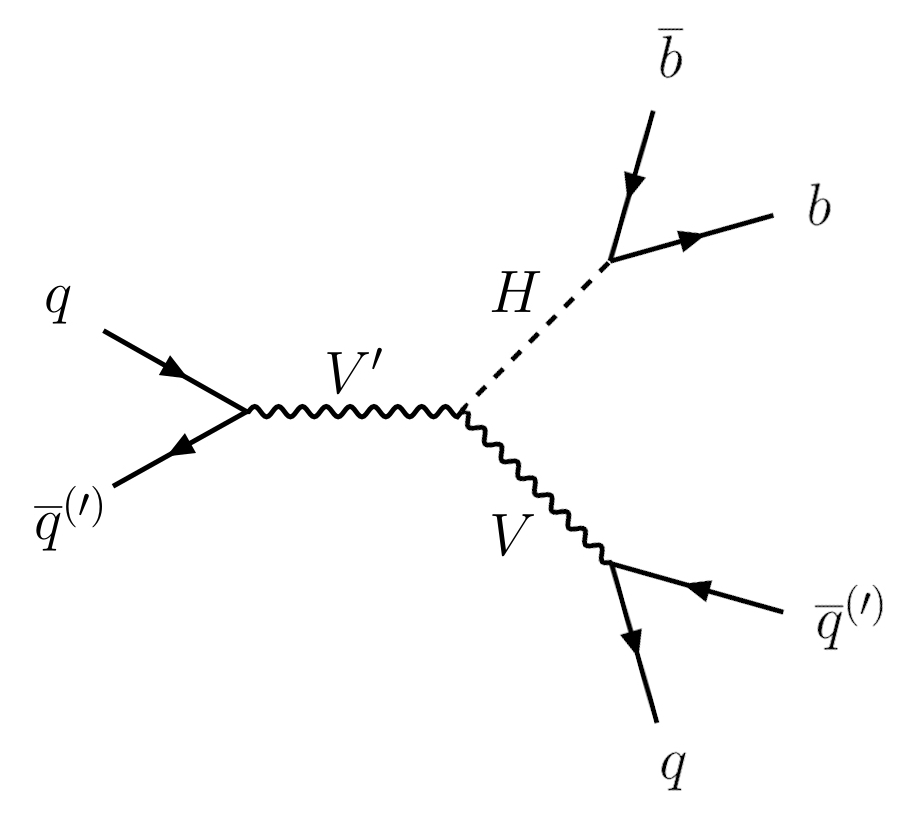
\includegraphics[width=0.65\textwidth,origin=c]{VH____qqbb_Feynman_Diagram}
	\caption{
	Feynman diagram illustrating the $pp \rightarrow V^\prime \rightarrow VH$ production/decay chain searched for by this analysis.
	The initial state quarks originate from the two protons involved in the hard scatter event.
	}
	\label{fig:feynman_diagram_VHqqbb}
\end{figure}

The $V$ and $H$ bosons that are produced in the decay of such theoretical heavy resonances are highly boosted and the resulting decay products of each boson are likely to be collimated and merged into a single large radius jet.
The dijet invariant mass ($m_{JJ}$) spectrum of the two large radius jets is then used as the discriminant variable, where the signature of the new heavy resonance decay yields a resonant peak structure on top of the smoothly falling background.
The dominant background ($\approx$ 90\%) corresponds to multijet QCD processes, with much smaller contributions from other non-resonant SM backgrounds: $t\bar{t}$ and $V$ + jets.
After reconstructing the $V$ and $H$ boson candidates as large radius jets, the tools of jet substructure (Section~\ref{sec:jet_substructure}) and b-tagging (Section~\ref{sec:btagging}) are applied to heavily suppress the dominant background of multijet events.
Due to the challenges associated with modelling this background with MC simulated samples, a fully data-driven method is used to provide a background estimation method.

A simplified theoretical model \cite{Pappadopulo:2014qza} fulfilling only SM symmetry constraints is used to provide a model-independent Lagrangian for a heavy resonance search.
This framework incorporates Heavy Vector Triplets (HVT), a common SM extension with an isospin $SU(2)_{L}$ triplet formed of a neutral $Z'$ and two charged $W^{\prime \pm}$ bosons, from which two explicit models will be considered as benchmarks to evaluate the relative sensitivity of this analysis to $W^{\prime \pm}$ and $Z'$ signals: Models A and B \cite{Pappadopulo:2014qza}, where weakly and strongly coupling scenarios are described, respectively.
The couplings of the new vector bosons $W^{\prime \pm}$, $Z'$ to the $H$ and $V$ bosons are defined as a combination of parameters $g_{V}c_{H}$, while the couplings to fermions are defined as $(g^{2}/g_{V})c_{F}$, where $g_V$ represents the strength of the new vector boson interaction and $c_{H}$ ($c_{F}$) represents the coupling to the Higgs boson (fermions).
In Model A, the branching fractions to fermions and gauge bosons are comparable, whereas in Model B the fermionic couplings are suppressed.

A search for heavy vector resonances decaying to $VH$ in the fully hadronic final state was previously performed in ATLAS using $36.1\pm1.0\text{~fb}^{-1}$ of $pp$ collision data at 13 TeV taken during 2015 and 2016 \cite{Aaboud:2017ahz}.
The largest excess was observed in the $ZH$ channel at $m_{JJ}\sim3.0$~TeV with a local significance of 3.3~$\sigma$, and a  global significance of  2.2~$\sigma$.
Upper limits on the production cross-section times branching ratio to the $q\bar{q}^{(\prime)}b\bar{b}$ final state were set for resonance masses in the range between 1000 and 3800 GeV with values ranging between 107 to 3 fb and 97 to 2 fb (at 95\% CL) for $WH$ and $ZH$ resonances, respectively.
The corresponding excluded HVT Model B signal mass ranges are 1000-2500 GeV for $WH$ resonances, and 1000 - 2600 GeV for $ZH$ resonances.

Searches for heavy vector resonances decaying to $VH$ in the $V$ boson leptonic decay channels have been performed in ATLAS using $36.1\pm1.0\text{~fb}^{-1}$ of $pp$ collision data at 13 TeV \cite{EXOT-2016-10}.
For HVT Model A $W'$ ($Z'$) masses have been excluded up to 2.67 TeV (2.65 TeV), while for Model B, $W'$ ($Z'$) masses of up to 2.86 TeV (2.83 TeV) have been excluded.

The CMS collaboration has published a search for new heavy resonances decaying to $VH$ in the fully hadronic mode using $19.7$~fb$^{-1}$ of 8 TeV data from Run 1 of the LHC.
Resonance masses up to 1.7 TeV were excluded in the combined $W'$ and $Z'$ search (1.1 TeV in \zpzh, 1.5 TeV in \wpwh), using the HVT Model B benchmark \cite{Khachatryan:2015bma}.
The search was also performed by CMS using $35.9$~fb$^{-1}$ of 13 TeV data from Run 2 of the LHC, excluding $W'$ ($Z'$) bosons with masses up to 3.15 TeV (2.26 TeV, except 1.19-1.21 TeV) in Model B \cite{Sirunyan:2017wto}.

% TODO: adapt this summary to thesis .tex structure
This chapter is structured as follows: Section \ref{sec:theory_overview} describes the contents and motivation behind the HVT model; Section \ref{sec:samples} describes the data and simulated samples used; Sections \ref{sec:objects} and \ref{sec:selection} describe the object definitions, event selection criteria and corresponding optimization studies; Section \ref{sec:background} describes the strategy for background estimation; Section \ref{sec:statistics} describes the statistical method used to interpret the results; Section \ref{sec:syst} describes the systematic uncertainties considered in this search.
The results and conclusions of the search are provided in Chapter \ref{ch:results}.

\section{Theoretical Framework/Motivation}
\label{sec:theory_overview}

In order to search for any BSM signature in a particle collider experiment, a model with explicit predictions is necessary.
No particular model has emerged as the most compelling or well-motivated possibility to single out for search efforts, but producing explicit results\footnote{A \textit{result} here consists of a set of experimentally-derived statistical constraints on model parameters related to the heavy resonance.} for each model would be prohibitively difficult and time consuming for HEP researchers.
However, the case of a heavy resonance search simplifies the matter because it is not sensitive to all the specific details and free parameters of any underlying model, but only the restricted set of parameters which control the mass of the resonance and any interactions involved in its production and decay.

For this reason a so-called \textit{bridge model} has been developed called the Heavy Vector Triplet (HVT) model \cite{Pappadopulo:2014qza}.
It employs a simplified model of the resonance where only the mass parameters and relevant couplings to SM particles are retained.
Aside from known SM symmetry constraints this simplified Lagrangian model does not need to fulfill any particular theoretical requirements.
With this simplified model, experimental results can be presented only in terms of the parameter space of this simplified Lagrangian.
In this way experimental results can be easily translated by theorists into constraints on parameters of any particular model.
Due to the careful construction of the HVT model this can be done analytically and not just via numerical simulations, which eliminates the need for knowledge (on the theorists part) of the experimental details of the search results.

Conceptually this method can be represented by a bridge as seen in Figure~\ref{fig:hvt_bridge}.
The central pillar represents the simplified model with Lagrangian $\mathcal{L}_S$ and parameters $\vec{c}$.
The likelihood $L(\vec{c})$ is used by the experimental analysis (see Section \ref{sec:statistics}) to derive constraints on the simplified model parameters $\vec{c}$.
Once the experimental constraints on $\vec{c}$ are known they can be translated into the free parameters $\vec{p}$ of any explicit theoretical model by computing their analytic relationship to the simplified model parameters: $\vec{c}(\vec{p})$.

\begin{figure}
	\centering
	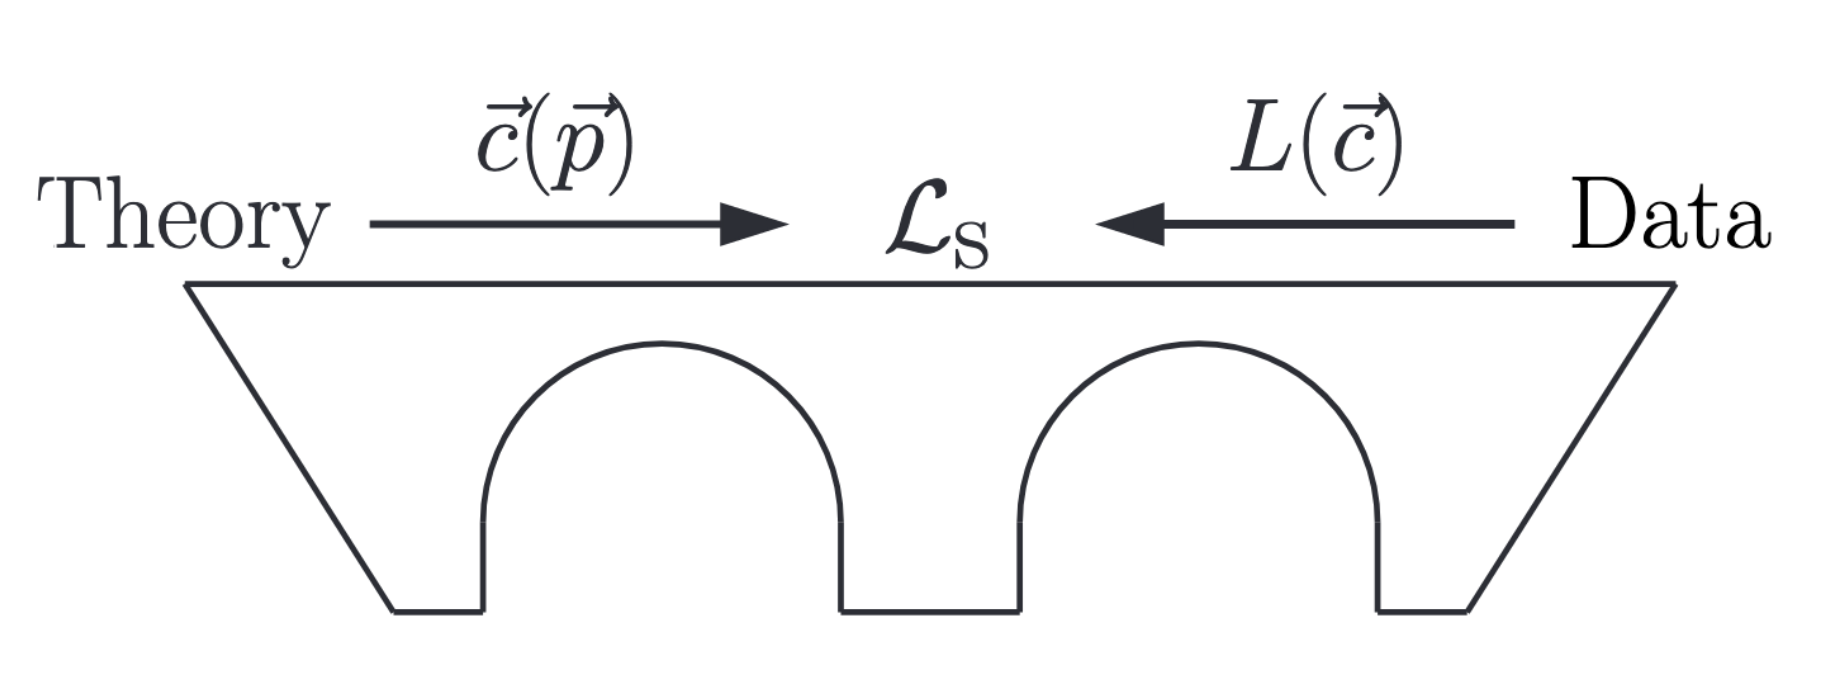
\includegraphics[width=0.65\textwidth,origin=c]{hvt_bridge}
	\caption{
	Pictorial view of the HVT bridge method. \cite{Pappadopulo:2014qza}
	}
	\label{fig:hvt_bridge}
\end{figure}

Due to its nature as a simplified model rather than a complete description of Nature, some care must be taken to ensure the HVT model is not applied outside the realm of its validity.
Most importantly the HVT model is constructed to only describe \textit{on-shell} resonance production and decay.
Thus a corresponding experimental search should only be sensitive to the on-shell process and insensitive to any off-shell effects.

The HVT model Lagrangian is constructed beginning with the SM Lagrangian and incorporating a real vector $V_\mu^a$, $a=1,2,3$, in the adjoint representation of $SU(2)_L$ with vanishing hypercharge.
These new additions describe two charged ($V_\mu^\pm$) and one neutral ($V_\mu^0$) heavy spin-one particles with the charge eigenstate fields defined by the following relations
\begin{equation}
V_\mu^\pm = \frac{V_\mu^1 \mp iV_\mu^2}{\sqrt{2}},\ \ \ V_\mu^0 = V_\mu^3.
\end{equation}

\begin{table}[!htb]
\begin{center}
\begin{tabular}{|c|c|}
\hline
$W$ Boson Property & Measured Value \\ \hline
mass & 80.379 $\pm$ 0.012 GeV \\
\hline
$\Gamma_{\mathrm{total}}$ & 2.085 $\pm$ 0.042 GeV \\
$\Gamma(e^+ \bar{\nu}_e) / \Gamma_{\mathrm{total}}$ & 10.71 $\pm$ 0.16 [\%]\\
$\Gamma(\mu^+ \bar{\nu}_\mu) / \Gamma_{\mathrm{total}}$ & 10.63 $\pm$ 0.15 [\%]\\
$\Gamma(\tau^+ \bar{\nu}_\tau) / \Gamma_{\mathrm{total}}$ & 11.38 $\pm$ 0.21 [\%]\\
$\Gamma(\mathrm{hadrons}) / \Gamma_{\mathrm{total}}$ & 67.41 $\pm$ 0.27 [\%]\\
\hline
$\langle N_{\mathrm{charged}} \rangle$ & 19.39 $\pm$ 0.08 \\
\hline
\end{tabular}
\caption{
W Boson properties computed from global averages of experimental results by the Particle Data Group (PDG). \cite{PDG:PhysRevD.98.030001}
}
\label{tab:w_props}
\end{center}
\end{table}

\begin{table}[!htb]
\begin{center}
\begin{tabular}{|c|c|}
\hline
$Z$ Boson Property & Measured Value \\ \hline
mass & 91.1876 $\pm$ 0.0021 GeV \\
\hline
$\Gamma_{\mathrm{total}}$ & 2.4952 $\pm$ 0.0023 GeV \\
$\Gamma(e^+ e^-) / \Gamma_{\mathrm{total}}$ & 3.3632 $\pm$ 0.0042 [\%]\\
$\Gamma(\mu^+ \mu^-) / \Gamma_{\mathrm{total}}$ & 3.3662 $\pm$ 0.0066 [\%]\\
$\Gamma(\tau^+ \tau^-) / \Gamma_{\mathrm{total}}$ & 3.3696 $\pm$ 0.0083 [\%]\\
$\Gamma(\mathrm{invisible}) / \Gamma_{\mathrm{total}}$ & 20.000 $\pm$ 0.055 [\%]\\
$\Gamma(\mathrm{hadrons}) / \Gamma_{\mathrm{total}}$ & 69.911 $\pm$ 0.056 [\%]\\
\hline
$\langle N_{\mathrm{charged}} \rangle$ & 20.76 $\pm$ 0.16 \\
\hline
\end{tabular}
\caption{
Z Boson properties computed from global averages of experimental results by the Particle Data Group (PDG). \cite{PDG:PhysRevD.98.030001}
}
\label{tab:z_props}
\end{center}
\end{table}

\begin{figure}
	\centering
	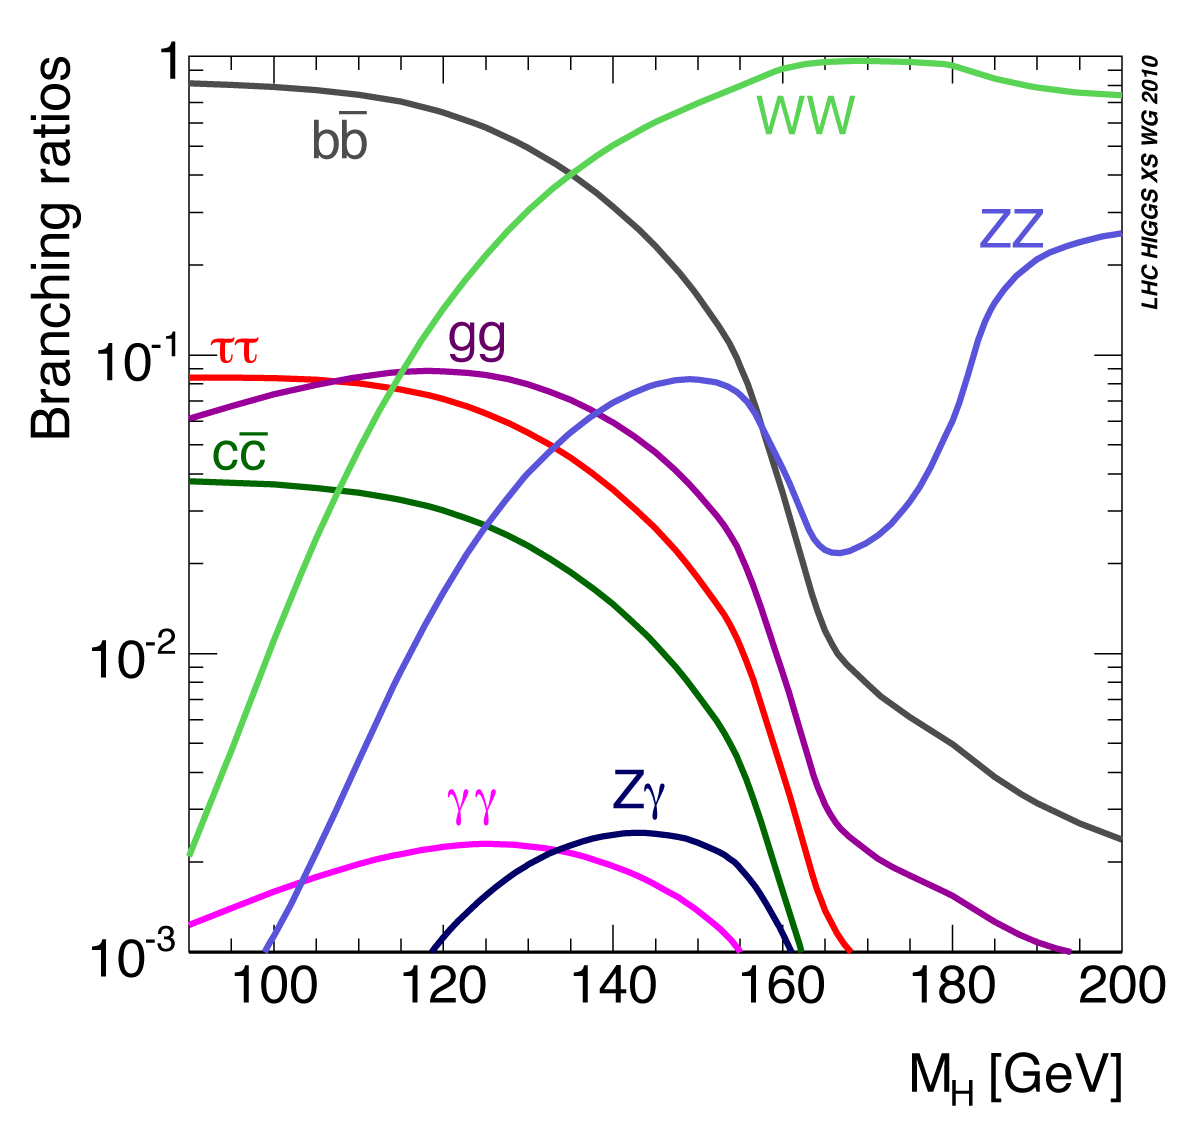
\includegraphics[width=0.65\textwidth,origin=c]{h_branching_ratios}
	\caption{
	Standard Model predictions for Higgs boson decay branching ratios. \cite{Dittmaier:2012vm}
	}
	\label{fig:h_branching_ratios}
\end{figure}

% \begin{figure}
% 	\centering
% 	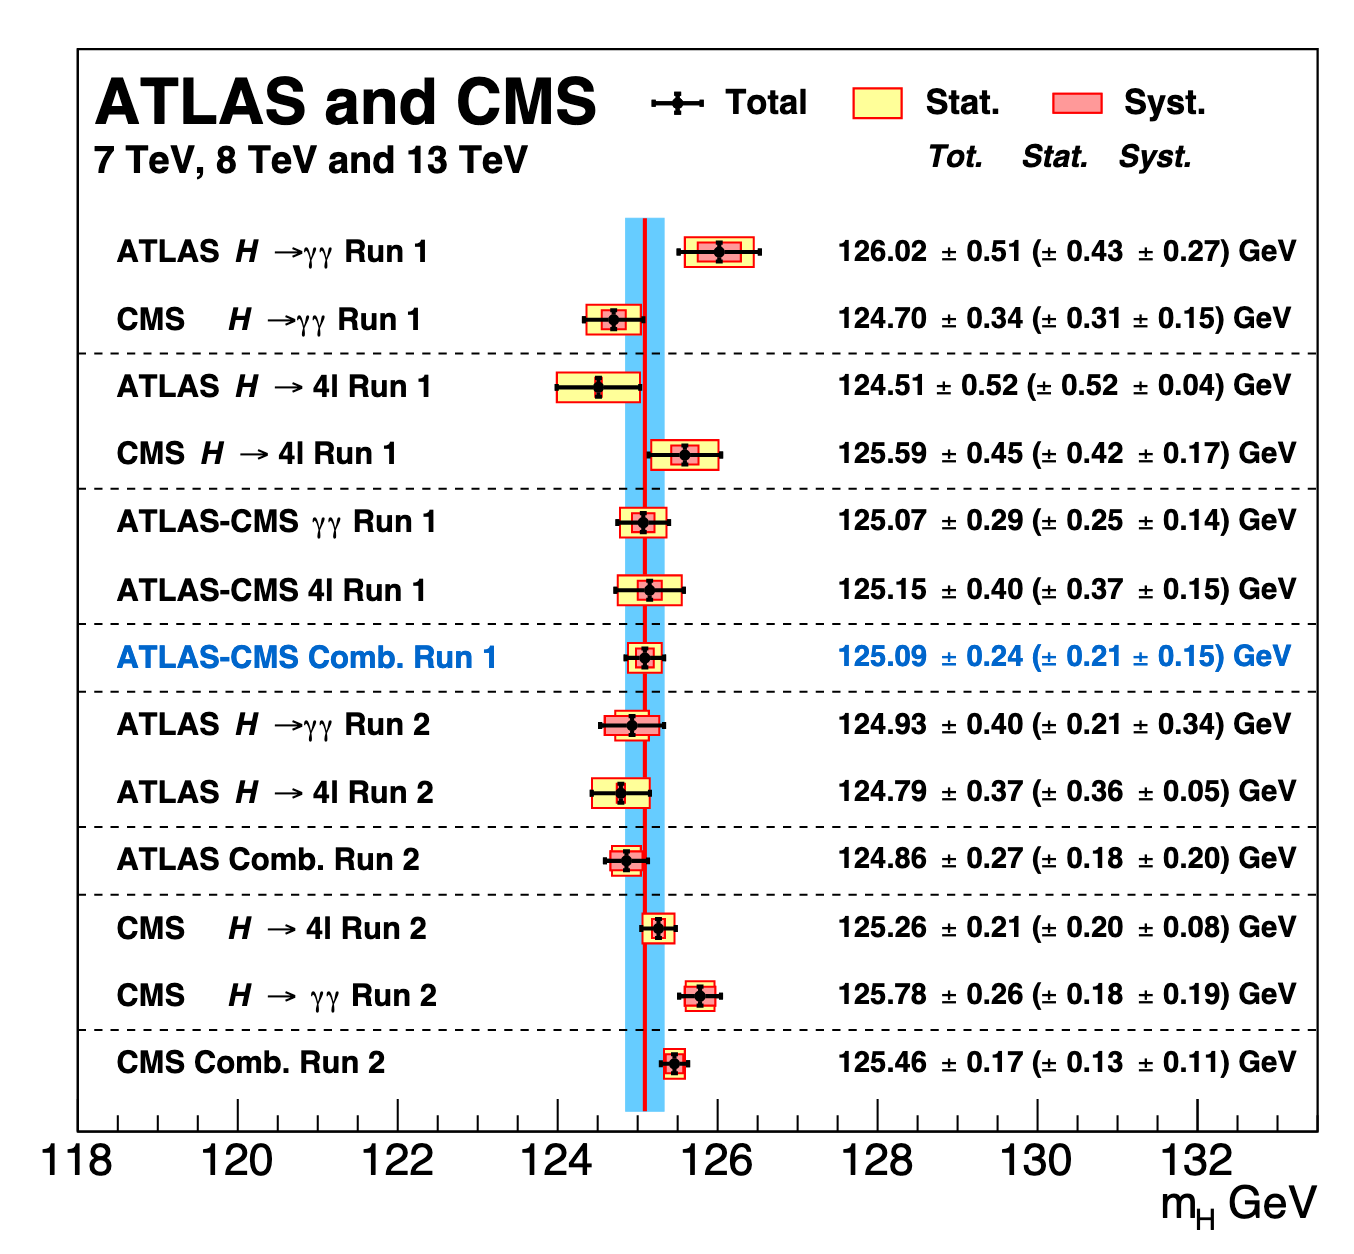
\includegraphics[width=0.85\textwidth,origin=c]{h_boson_mass_measurement_LHC}
% 	\caption{
% 	Summary of the ATLAS and CMS $H^0$ mass measurements in the $\gamma\gamma$ and $ZZ \rightarrow 4 \mathrm{lepton}$ channels for Run-1 and Run-2.
% 	\cite{Aad:2015zhl, Aaboud:2018wps, Sirunyan:2017exp}
% 	}
% 	\label{fig:h_mass_measurement}
% \end{figure}

\section{Data and Monte Carlo Simulation}
\label{sec:samples}

% Possible Feynman Diagrams: https://www-d0.fnal.gov/Run2Physics/top/top_public_web_pages/top_feynman_diagrams.html

\subsection{Signal}
The Heavy Vector Triplet (HVT) Model A with $g_{V}=1$ samples are used as a benchmark model to interpret the results of this analysis.
Under the assumption that there are no differences\footnote{The width of the HVT resonance is dominated entirely by experimental resolution} between Model A and Model B in terms of the relevant kinematics of the event, the results interpreted with the Model A samples can be directly translated to Model B by scaling the relevant branching fraction and cross section values.
The MC samples are generated at leading order in $\alpha_S$ with \MADGRAPH5\_aMC@NLO 2.2.2 \cite{Alwall:2014hca} interfaced to \PYTHIA8.186 \cite{Sjostrand:2007gs} for parton shower and hadronization, with the NNPDF23 PDF set \cite{Ball:2011mu} and the ATLAS A14 tune \cite{ATL-PHYS-PUB-2014-021}. Tables \ref{tab:hvta_wh} and \ref{tab:hvta_zh} show the cross-sections and sample information for the HVT Model A samples, generated at different mass points in the range of 1 to 5 TeV.
Only \Hbb and $H\rightarrow c\bar{c}$ decays are included for the Higgs boson, corresponding to a branching ratio of 0.569 + 0.0287 \cite{Aad:2015gba}.
Tables~\ref{tab:hvta_wh} and ~\ref{tab:hvta_zh} summarize the properties of the HVT Model A signal samples generated and used for this analysis, while Tables~\ref{tab:hvtb_wh} and ~\ref{tab:hvtb_zh} describe HVT Model B.

\begin{table}[!htb]
\begin{scriptsize}
\begin{center}
\begin{tabular}{|c|l|c|c|c|c|r|}
\hline
DSID & Process & Generator & $\sigma$ [fb] & $k$-factor & $\epsilon_{\text{filter}}$ & Events \\ \hline
302321 & \makecell{HVT $W^{\prime} \rightarrow WH \rightarrow qq^\prime(b\bar{b} + c\bar{c})$ \\ Model A, m = 1000 GeV} & \makecell{\MADGRAPH v2.2.2 + \PYTHIA v8.186 \\ + EvtGen v1.2.0} & 4.334e+02 & 1.0 & 1.0 & 110000 \\
\hline
302322 & \makecell{HVT $W^{\prime} \rightarrow WH \rightarrow qq^\prime(b\bar{b} + c\bar{c})$ \\ Model A, m = 1100 GeV} & \makecell{\MADGRAPH v2.2.2 + \PYTHIA v8.186 \\ + EvtGen v1.2.0} & 2.901e+02 & 1.0 & 1.0 & 110000 \\
\hline
302323 & \makecell{HVT $W^{\prime} \rightarrow WH \rightarrow qq^\prime(b\bar{b} + c\bar{c})$ \\ Model A, m = 1200 GeV} & \makecell{\MADGRAPH v2.2.2 + \PYTHIA v8.186 \\ + EvtGen v1.2.0} & 1.995e+02 & 1.0 & 1.0 & 110000 \\
\hline
302324 & \makecell{HVT $W^{\prime} \rightarrow WH \rightarrow qq^\prime(b\bar{b} + c\bar{c})$ \\ Model A, m = 1300 GeV} & \makecell{\MADGRAPH v2.2.2 + \PYTHIA v8.186 \\ + EvtGen v1.2.0} & 1.401e+02 & 1.0 & 1.0 & 95000 \\
\hline
302325 & \makecell{HVT $W^{\prime} \rightarrow WH \rightarrow qq^\prime(b\bar{b} + c\bar{c})$ \\ Model A, m = 1400 GeV} & \makecell{\MADGRAPH v2.2.2 + \PYTHIA v8.186 \\ + EvtGen v1.2.0} & 1.002e+02 & 1.0 & 1.0 & 125000 \\
\hline
302326 & \makecell{HVT $W^{\prime} \rightarrow WH \rightarrow qq^\prime(b\bar{b} + c\bar{c})$ \\ Model A, m = 1500 GeV} & \makecell{\MADGRAPH v2.2.2 + \PYTHIA v8.186 \\ + EvtGen v1.2.0} & 7.283e+01 & 1.0 & 1.0 & 80000 \\
\hline
302327 & \makecell{HVT $W^{\prime} \rightarrow WH \rightarrow qq^\prime(b\bar{b} + c\bar{c})$ \\ Model A, m = 1600 GeV} & \makecell{\MADGRAPH v2.2.3 + \PYTHIA v8.186 \\ + EvtGen v1.2.0} & 5.367e+01 & 1.0 & 1.0 & 110000 \\
\hline
302328 & \makecell{HVT $W^{\prime} \rightarrow WH \rightarrow qq^\prime(b\bar{b} + c\bar{c})$ \\ Model A, m = 1700 GeV} & \makecell{\MADGRAPH v2.2.2 + \PYTHIA v8.186 \\ + EvtGen v1.2.0} & 3.999e+01 & 1.0 & 1.0 & 110000 \\
\hline
302329 & \makecell{HVT $W^{\prime} \rightarrow WH \rightarrow qq^\prime(b\bar{b} + c\bar{c})$ \\ Model A, m = 1800 GeV} & \makecell{\MADGRAPH v2.2.3 + \PYTHIA v8.186 \\ + EvtGen v1.2.0} & 3.012e+01 & 1.0 & 1.0 & 110000 \\
\hline
302330 & \makecell{HVT $W^{\prime} \rightarrow WH \rightarrow qq^\prime(b\bar{b} + c\bar{c})$ \\ Model A, m = 1900 GeV} & \makecell{\MADGRAPH v2.2.2 + \PYTHIA v8.186 \\ + EvtGen v1.2.0} & 2.289e+01 & 1.0 & 1.0 & 70000 \\
\hline
302331 & \makecell{HVT $W^{\prime} \rightarrow WH \rightarrow qq^\prime(b\bar{b} + c\bar{c})$ \\ Model A, m = 2000 GeV} & \makecell{\MADGRAPH v2.2.2 + \PYTHIA v8.186 \\ + EvtGen v1.2.0} & 1.753e+01 & 1.0 & 1.0 & 105000 \\
\hline
302332 & \makecell{HVT $W^{\prime} \rightarrow WH \rightarrow qq^\prime(b\bar{b} + c\bar{c})$ \\ Model A, m = 2200 GeV} & \makecell{\MADGRAPH v2.2.2 + \PYTHIA v8.186 \\ + EvtGen v1.2.0} & 1.049e+01 & 1.0 & 1.0 & 110000 \\
\hline
302333 & \makecell{HVT $W^{\prime} \rightarrow WH \rightarrow qq^\prime(b\bar{b} + c\bar{c})$ \\ Model A, m = 2400 GeV} & \makecell{\MADGRAPH v2.2.2 + \PYTHIA v8.186 \\ + EvtGen v1.2.0} & 6.427e+00 & 1.0 & 1.0 & 110000 \\
\hline
302334 & \makecell{HVT $W^{\prime} \rightarrow WH \rightarrow qq^\prime(b\bar{b} + c\bar{c})$ \\ Model A, m = 2600 GeV} & \makecell{\MADGRAPH v2.2.2 + \PYTHIA v8.186 \\ + EvtGen v1.2.0} & 4.008e+00 & 1.0 & 1.0 & 110000 \\
\hline
302335 & \makecell{HVT $W^{\prime} \rightarrow WH \rightarrow qq^\prime(b\bar{b} + c\bar{c})$ \\ Model A, m = 2800 GeV} & \makecell{\MADGRAPH v2.2.2 + \PYTHIA v8.186 \\ + EvtGen v1.2.0} & 2.537e+00 & 1.0 & 1.0 & 110000 \\
\hline
302336 & \makecell{HVT $W^{\prime} \rightarrow WH \rightarrow qq^\prime(b\bar{b} + c\bar{c})$ \\ Model A, m = 3000 GeV} & \makecell{\MADGRAPH v2.2.2 + \PYTHIA v8.186 \\ + EvtGen v1.2.0} & 1.624e+00 & 1.0 & 1.0 & 50000 \\
\hline
302337 & \makecell{HVT $W^{\prime} \rightarrow WH \rightarrow qq^\prime(b\bar{b} + c\bar{c})$ \\ Model A, m = 3500 GeV} & \makecell{\MADGRAPH v2.2.2 + \PYTHIA v8.186 \\ + EvtGen v1.2.0} & 5.534e-01 & 1.0 & 1.0 & 65000 \\
\hline
302338 & \makecell{HVT $W^{\prime} \rightarrow WH \rightarrow qq^\prime(b\bar{b} + c\bar{c})$ \\ Model A, m = 4000 GeV} & \makecell{\MADGRAPH v2.2.2 + \PYTHIA v8.186 \\ + EvtGen v1.2.0} & 1.953e-01 & 1.0 & 1.0 & 100000 \\
\hline
302339 & \makecell{HVT $W^{\prime} \rightarrow WH \rightarrow qq^\prime(b\bar{b} + c\bar{c})$ \\ Model A, m = 4500 GeV} & \makecell{\MADGRAPH v2.2.2 + \PYTHIA v8.186 \\ + EvtGen v1.2.0} & 7.015e-02 & 1.0 & 1.0 & 80000 \\
\hline
302340 & \makecell{HVT $W^{\prime} \rightarrow WH \rightarrow qq^\prime(b\bar{b} + c\bar{c})$ \\ Model A, m = 5000 GeV} & \makecell{\MADGRAPH v2.2.2 + \PYTHIA v8.186 \\ + EvtGen v1.2.0} & 2.543e-02 & 1.0 & 1.0 & 85000 \\
\hline
\end{tabular}
\caption{
    HVT Model A ($g_V=1$) WH samples used in the analysis. The dataset ID, MC generator, production cross-sections,
    $k$-factor, filter efficiency and total number of generated events are shown.
}
\label{tab:hvta_wh}
\end{center}
\end{scriptsize}
\end{table}

\begin{table}[!htb]
\begin{scriptsize}
\begin{center}
\begin{tabular}{|c|l|c|c|c|c|r|}
\hline
DSID & Process & Generator & $\sigma$ [fb] & $k$-factor & $\epsilon_{\text{filter}}$ & Events \\ \hline
302371 & \makecell{HVT $Z^{\prime} \rightarrow ZH \rightarrow q\bar{q}(b\bar{b} + c\bar{c})$ \\ Model A, m = 1000 GeV} & \makecell{\MADGRAPH v2.2.2 + \PYTHIA v8.186 \\ + EvtGen v1.2.0} & 2.179e+02 & 1.0 & 1.0 & 50000 \\
\hline
302372 & \makecell{HVT $Z^{\prime} \rightarrow ZH \rightarrow q\bar{q}(b\bar{b} + c\bar{c})$ \\ Model A, m = 1100 GeV} & \makecell{\MADGRAPH v2.2.3 + \PYTHIA v8.186 \\ + EvtGen v1.2.0} & 1.446e+02 & 1.0 & 1.0 & 110000 \\
\hline
302373 & \makecell{HVT $Z^{\prime} \rightarrow ZH \rightarrow q\bar{q}(b\bar{b} + c\bar{c})$ \\ Model A, m = 1200 GeV} & \makecell{\MADGRAPH v2.2.2 + \PYTHIA v8.186 \\ + EvtGen v1.2.0} & 9.855e+01 & 1.0 & 1.0 & 80000 \\
\hline
302374 & \makecell{HVT $Z^{\prime} \rightarrow ZH \rightarrow q\bar{q}(b\bar{b} + c\bar{c})$ \\ Model A, m = 1300 GeV} & \makecell{\MADGRAPH v2.2.2 + \PYTHIA v8.186 \\ + EvtGen v1.2.0} & 6.871e+01 & 1.0 & 1.0 & 70000 \\
\hline
302375 & \makecell{HVT $Z^{\prime} \rightarrow ZH \rightarrow q\bar{q}(b\bar{b} + c\bar{c})$ \\ Model A, m = 1400 GeV} & \makecell{\MADGRAPH v2.2.2 + \PYTHIA v8.186 \\ + EvtGen v1.2.0} & 4.881e+01 & 1.0 & 1.0 & 95000 \\
\hline
302376 & \makecell{HVT $Z^{\prime} \rightarrow ZH \rightarrow q\bar{q}(b\bar{b} + c\bar{c})$ \\ Model A, m = 1500 GeV} & \makecell{\MADGRAPH v2.2.2 + \PYTHIA v8.186 \\ + EvtGen v1.2.0} & 3.525e+01 & 1.0 & 1.0 & 100000 \\
\hline
302377 & \makecell{HVT $Z^{\prime} \rightarrow ZH \rightarrow q\bar{q}(b\bar{b} + c\bar{c})$ \\ Model A, m = 1600 GeV} & \makecell{\MADGRAPH v2.2.2 + \PYTHIA v8.186 \\ + EvtGen v1.2.0} & 2.581e+01 & 1.0 & 1.0 & 55000 \\
\hline
302378 & \makecell{HVT $Z^{\prime} \rightarrow ZH \rightarrow q\bar{q}(b\bar{b} + c\bar{c})$ \\ Model A, m = 1700 GeV} & \makecell{\MADGRAPH v2.2.3 + \PYTHIA v8.186 \\ + EvtGen v1.2.0} & 1.913e+01 & 1.0 & 1.0 & 110000 \\
\hline
302379 & \makecell{HVT $Z^{\prime} \rightarrow ZH \rightarrow q\bar{q}(b\bar{b} + c\bar{c})$ \\ Model A, m = 1800 GeV} & \makecell{\MADGRAPH v2.2.2 + \PYTHIA v8.186 \\ + EvtGen v1.2.0} & 1.434e+01 & 1.0 & 1.0 & 104000 \\
\hline
302380 & \makecell{HVT $Z^{\prime} \rightarrow ZH \rightarrow q\bar{q}(b\bar{b} + c\bar{c})$ \\ Model A, m = 1900 GeV} & \makecell{\MADGRAPH v2.2.2 + \PYTHIA v8.186 \\ + EvtGen v1.2.0} & 1.084e+01 & 1.0 & 1.0 & 95000 \\
\hline
302381 & \makecell{HVT $Z^{\prime} \rightarrow ZH \rightarrow q\bar{q}(b\bar{b} + c\bar{c})$ \\ Model A, m = 2000 GeV} & \makecell{\MADGRAPH v2.2.2 + \PYTHIA v8.186 \\ + EvtGen v1.2.0} & 8.271e+00 & 1.0 & 1.0 & 110000 \\
\hline
302382 & \makecell{HVT $Z^{\prime} \rightarrow ZH \rightarrow q\bar{q}(b\bar{b} + c\bar{c})$ \\ Model A, m = 2200 GeV} & \makecell{\MADGRAPH v2.2.2 + \PYTHIA v8.186 \\ + EvtGen v1.2.0} & 4.916e+00 & 1.0 & 1.0 & 85000 \\
\hline
302383 & \makecell{HVT $Z^{\prime} \rightarrow ZH \rightarrow q\bar{q}(b\bar{b} + c\bar{c})$ \\ Model A, m = 2400 GeV} & \makecell{\MADGRAPH v2.2.3 + \PYTHIA v8.186 \\ + EvtGen v1.2.0} & 2.994e+00 & 1.0 & 1.0 & 110000 \\
\hline
302384 & \makecell{HVT $Z^{\prime} \rightarrow ZH \rightarrow q\bar{q}(b\bar{b} + c\bar{c})$ \\ Model A, m = 2600 GeV} & \makecell{\MADGRAPH v2.2.2 + \PYTHIA v8.186 \\ + EvtGen v1.2.0} & 1.859e+00 & 1.0 & 1.0 & 105000 \\
\hline
302385 & \makecell{HVT $Z^{\prime} \rightarrow ZH \rightarrow q\bar{q}(b\bar{b} + c\bar{c})$ \\ Model A, m = 2800 GeV} & \makecell{\MADGRAPH v2.2.2 + \PYTHIA v8.186 \\ + EvtGen v1.2.0} & 1.173e+00 & 1.0 & 1.0 & 70000 \\
\hline
302386 & \makecell{HVT $Z^{\prime} \rightarrow ZH \rightarrow q\bar{q}(b\bar{b} + c\bar{c})$ \\ Model A, m = 3000 GeV} & \makecell{\MADGRAPH v2.2.2 + \PYTHIA v8.186 \\ + EvtGen v1.2.0} & 7.497e-01 & 1.0 & 1.0 & 90000 \\
\hline
302387 & \makecell{HVT $Z^{\prime} \rightarrow ZH \rightarrow q\bar{q}(b\bar{b} + c\bar{c})$ \\ Model A, m = 3500 GeV} & \makecell{\MADGRAPH v2.2.2 + \PYTHIA v8.186 \\ + EvtGen v1.2.0} & 2.554e-01 & 1.0 & 1.0 & 110000 \\
\hline
302388 & \makecell{HVT $Z^{\prime} \rightarrow ZH \rightarrow q\bar{q}(b\bar{b} + c\bar{c})$ \\ Model A, m = 4000 GeV} & \makecell{\MADGRAPH v2.2.2 + \PYTHIA v8.186 \\ + EvtGen v1.2.0} & 9.049e-02 & 1.0 & 1.0 & 75000 \\
\hline
302389 & \makecell{HVT $Z^{\prime} \rightarrow ZH \rightarrow q\bar{q}(b\bar{b} + c\bar{c})$ \\ Model A, m = 4500 GeV} & \makecell{\MADGRAPH v2.2.2 + \PYTHIA v8.186 \\ + EvtGen v1.2.0} & 3.274e-02 & 1.0 & 1.0 & 100000 \\
\hline
302390 & \makecell{HVT $Z^{\prime} \rightarrow ZH \rightarrow q\bar{q}(b\bar{b} + c\bar{c})$ \\ Model A, m = 5000 GeV} & \makecell{\MADGRAPH v2.2.2 + \PYTHIA v8.186 \\ + EvtGen v1.2.0} & 1.198e-02 & 1.0 & 1.0 & 110000 \\
\hline
\end{tabular}
\caption{
    HVT Model A ($g_V=1$) ZH samples used in the analysis. The dataset ID, MC generator, production cross-sections,
    $k$-factor, filter efficiency and total number of generated events are shown.
}
\label{tab:hvta_zh}
\end{center}
\end{scriptsize}
\end{table}

\begin{table}[!htb]
\begin{scriptsize}
\begin{center}
\begin{tabular}{|c|l|c|c|c|c|r|}
\hline
DSID & Process & Generator & $\sigma$ [fb] & $k$-factor & $\epsilon_{\text{filter}}$ & Events \\ \hline
302321 & \makecell{HVT $W^{\prime} \rightarrow WH \rightarrow qq^\prime(b\bar{b} + c\bar{c})$ \\ Model B, m = 1000 GeV} & \makecell{\MADGRAPH v2.2.2 + \PYTHIA v8.186 \\ + EvtGen v1.2.0} & 5.016e+02 & 1.0 & 1.0 & 110000 \\
\hline
302322 & \makecell{HVT $W^{\prime} \rightarrow WH \rightarrow qq^\prime(b\bar{b} + c\bar{c})$ \\ Model B, m = 1100 GeV} & \makecell{\MADGRAPH v2.2.2 + \PYTHIA v8.186 \\ + EvtGen v1.2.0} & 3.634e+02 & 1.0 & 1.0 & 110000 \\
\hline
302323 & \makecell{HVT $W^{\prime} \rightarrow WH \rightarrow qq^\prime(b\bar{b} + c\bar{c})$ \\ Model B, m = 1200 GeV} & \makecell{\MADGRAPH v2.2.2 + \PYTHIA v8.186 \\ + EvtGen v1.2.0} & 2.646e+02 & 1.0 & 1.0 & 110000 \\
\hline
302324 & \makecell{HVT $W^{\prime} \rightarrow WH \rightarrow qq^\prime(b\bar{b} + c\bar{c})$ \\ Model B, m = 1300 GeV} & \makecell{\MADGRAPH v2.2.2 + \PYTHIA v8.186 \\ + EvtGen v1.2.0} & 1.943e+02 & 1.0 & 1.0 & 95000 \\
\hline
302325 & \makecell{HVT $W^{\prime} \rightarrow WH \rightarrow qq^\prime(b\bar{b} + c\bar{c})$ \\ Model B, m = 1400 GeV} & \makecell{\MADGRAPH v2.2.2 + \PYTHIA v8.186 \\ + EvtGen v1.2.0} & 1.440e+02 & 1.0 & 1.0 & 125000 \\
\hline
302326 & \makecell{HVT $W^{\prime} \rightarrow WH \rightarrow qq^\prime(b\bar{b} + c\bar{c})$ \\ Model B, m = 1500 GeV} & \makecell{\MADGRAPH v2.2.2 + \PYTHIA v8.186 \\ + EvtGen v1.2.0} & 1.077e+02 & 1.0 & 1.0 & 80000 \\
\hline
302327 & \makecell{HVT $W^{\prime} \rightarrow WH \rightarrow qq^\prime(b\bar{b} + c\bar{c})$ \\ Model B, m = 1600 GeV} & \makecell{\MADGRAPH v2.2.3 + \PYTHIA v8.186 \\ + EvtGen v1.2.0} & 8.128e+01 & 1.0 & 1.0 & 110000 \\
\hline
302328 & \makecell{HVT $W^{\prime} \rightarrow WH \rightarrow qq^\prime(b\bar{b} + c\bar{c})$ \\ Model B, m = 1700 GeV} & \makecell{\MADGRAPH v2.2.2 + \PYTHIA v8.186 \\ + EvtGen v1.2.0} & 6.181e+01 & 1.0 & 1.0 & 110000 \\
\hline
302329 & \makecell{HVT $W^{\prime} \rightarrow WH \rightarrow qq^\prime(b\bar{b} + c\bar{c})$ \\ Model B, m = 1800 GeV} & \makecell{\MADGRAPH v2.2.3 + \PYTHIA v8.186 \\ + EvtGen v1.2.0} & 4.733e+01 & 1.0 & 1.0 & 110000 \\
\hline
302330 & \makecell{HVT $W^{\prime} \rightarrow WH \rightarrow qq^\prime(b\bar{b} + c\bar{c})$ \\ Model B, m = 1900 GeV} & \makecell{\MADGRAPH v2.2.2 + \PYTHIA v8.186 \\ + EvtGen v1.2.0} & 3.648e+01 & 1.0 & 1.0 & 70000 \\
\hline
302331 & \makecell{HVT $W^{\prime} \rightarrow WH \rightarrow qq^\prime(b\bar{b} + c\bar{c})$ \\ Model B, m = 2000 GeV} & \makecell{\MADGRAPH v2.2.2 + \PYTHIA v8.186 \\ + EvtGen v1.2.0} & 2.827e+01 & 1.0 & 1.0 & 105000 \\
\hline
302332 & \makecell{HVT $W^{\prime} \rightarrow WH \rightarrow qq^\prime(b\bar{b} + c\bar{c})$ \\ Model B, m = 2200 GeV} & \makecell{\MADGRAPH v2.2.2 + \PYTHIA v8.186 \\ + EvtGen v1.2.0} & 1.723e+01 & 1.0 & 1.0 & 110000 \\
\hline
302333 & \makecell{HVT $W^{\prime} \rightarrow WH \rightarrow qq^\prime(b\bar{b} + c\bar{c})$ \\ Model B, m = 2400 GeV} & \makecell{\MADGRAPH v2.2.2 + \PYTHIA v8.186 \\ + EvtGen v1.2.0} & 1.067e+01 & 1.0 & 1.0 & 110000 \\
\hline
302334 & \makecell{HVT $W^{\prime} \rightarrow WH \rightarrow qq^\prime(b\bar{b} + c\bar{c})$ \\ Model B, m = 2600 GeV} & \makecell{\MADGRAPH v2.2.2 + \PYTHIA v8.186 \\ + EvtGen v1.2.0} & 6.689e+00 & 1.0 & 1.0 & 110000 \\
\hline
302335 & \makecell{HVT $W^{\prime} \rightarrow WH \rightarrow qq^\prime(b\bar{b} + c\bar{c})$ \\ Model B, m = 2800 GeV} & \makecell{\MADGRAPH v2.2.2 + \PYTHIA v8.186 \\ + EvtGen v1.2.0} & 4.234e+00 & 1.0 & 1.0 & 110000 \\
\hline
302336 & \makecell{HVT $W^{\prime} \rightarrow WH \rightarrow qq^\prime(b\bar{b} + c\bar{c})$ \\ Model B, m = 3000 GeV} & \makecell{\MADGRAPH v2.2.2 + \PYTHIA v8.186 \\ + EvtGen v1.2.0} & 2.698e+00 & 1.0 & 1.0 & 50000 \\
\hline
302337 & \makecell{HVT $W^{\prime} \rightarrow WH \rightarrow qq^\prime(b\bar{b} + c\bar{c})$ \\ Model B, m = 3500 GeV} & \makecell{\MADGRAPH v2.2.2 + \PYTHIA v8.186 \\ + EvtGen v1.2.0} & 8.918e-01 & 1.0 & 1.0 & 65000 \\
\hline
302338 & \makecell{HVT $W^{\prime} \rightarrow WH \rightarrow qq^\prime(b\bar{b} + c\bar{c})$ \\ Model B, m = 4000 GeV} & \makecell{\MADGRAPH v2.2.2 + \PYTHIA v8.186 \\ + EvtGen v1.2.0} & 2.969e-01 & 1.0 & 1.0 & 100000 \\
\hline
302339 & \makecell{HVT $W^{\prime} \rightarrow WH \rightarrow qq^\prime(b\bar{b} + c\bar{c})$ \\ Model B, m = 4500 GeV} & \makecell{\MADGRAPH v2.2.2 + \PYTHIA v8.186 \\ + EvtGen v1.2.0} & 9.789e-02 & 1.0 & 1.0 & 80000 \\
\hline
302340 & \makecell{HVT $W^{\prime} \rightarrow WH \rightarrow qq^\prime(b\bar{b} + c\bar{c})$ \\ Model B, m = 5000 GeV} & \makecell{\MADGRAPH v2.2.2 + \PYTHIA v8.186 \\ + EvtGen v1.2.0} & 3.149e-02 & 1.0 & 1.0 & 85000 \\
\hline
\end{tabular}
\caption{
    HVT Model B ($g_V=3$) WH samples used in the analysis. The dataset ID, MC generator, production cross-sections,
    $k$-factor, filter efficiency and total number of generated events are shown.
}
\label{tab:hvtb_wh}
\end{center}
\end{scriptsize}
\end{table}

\begin{table}[!htb]
\begin{scriptsize}
\begin{center}
\begin{tabular}{|c|l|c|c|c|c|r|}
\hline
DSID & Process & Generator & $\sigma$ [fb] & $k$-factor & $\epsilon_{\text{filter}}$ & Events \\ \hline
302371 & \makecell{HVT $Z^{\prime} \rightarrow ZH \rightarrow q\bar{q}(b\bar{b} + c\bar{c})$ \\ Model B, m = 1000 GeV} & \makecell{\MADGRAPH v2.2.2 + \PYTHIA v8.186 \\ + EvtGen v1.2.0} & 2.641e+02 & 1.0 & 1.0 & 50000 \\
\hline
302372 & \makecell{HVT $Z^{\prime} \rightarrow ZH \rightarrow q\bar{q}(b\bar{b} + c\bar{c})$ \\ Model B, m = 1100 GeV} & \makecell{\MADGRAPH v2.2.3 + \PYTHIA v8.186 \\ + EvtGen v1.2.0} & 1.888e+02 & 1.0 & 1.0 & 110000 \\
\hline
302373 & \makecell{HVT $Z^{\prime} \rightarrow ZH \rightarrow q\bar{q}(b\bar{b} + c\bar{c})$ \\ Model B, m = 1200 GeV} & \makecell{\MADGRAPH v2.2.2 + \PYTHIA v8.186 \\ + EvtGen v1.2.0} & 1.358e+02 & 1.0 & 1.0 & 80000 \\
\hline
302374 & \makecell{HVT $Z^{\prime} \rightarrow ZH \rightarrow q\bar{q}(b\bar{b} + c\bar{c})$ \\ Model B, m = 1300 GeV} & \makecell{\MADGRAPH v2.2.2 + \PYTHIA v8.186 \\ + EvtGen v1.2.0} & 9.864e+01 & 1.0 & 1.0 & 70000 \\
\hline
302375 & \makecell{HVT $Z^{\prime} \rightarrow ZH \rightarrow q\bar{q}(b\bar{b} + c\bar{c})$ \\ Model B, m = 1400 GeV} & \makecell{\MADGRAPH v2.2.2 + \PYTHIA v8.186 \\ + EvtGen v1.2.0} & 7.236e+01 & 1.0 & 1.0 & 95000 \\
\hline
302376 & \makecell{HVT $Z^{\prime} \rightarrow ZH \rightarrow q\bar{q}(b\bar{b} + c\bar{c})$ \\ Model B, m = 1500 GeV} & \makecell{\MADGRAPH v2.2.2 + \PYTHIA v8.186 \\ + EvtGen v1.2.0} & 5.359e+01 & 1.0 & 1.0 & 100000 \\
\hline
302377 & \makecell{HVT $Z^{\prime} \rightarrow ZH \rightarrow q\bar{q}(b\bar{b} + c\bar{c})$ \\ Model B, m = 1600 GeV} & \makecell{\MADGRAPH v2.2.2 + \PYTHIA v8.186 \\ + EvtGen v1.2.0} & 4.006e+01 & 1.0 & 1.0 & 55000 \\
\hline
302378 & \makecell{HVT $Z^{\prime} \rightarrow ZH \rightarrow q\bar{q}(b\bar{b} + c\bar{c})$ \\ Model B, m = 1700 GeV} & \makecell{\MADGRAPH v2.2.3 + \PYTHIA v8.186 \\ + EvtGen v1.2.0} & 3.020e+01 & 1.0 & 1.0 & 110000 \\
\hline
302379 & \makecell{HVT $Z^{\prime} \rightarrow ZH \rightarrow q\bar{q}(b\bar{b} + c\bar{c})$ \\ Model B, m = 1800 GeV} & \makecell{\MADGRAPH v2.2.2 + \PYTHIA v8.186 \\ + EvtGen v1.2.0} & 2.292e+01 & 1.0 & 1.0 & 104000 \\
\hline
302380 & \makecell{HVT $Z^{\prime} \rightarrow ZH \rightarrow q\bar{q}(b\bar{b} + c\bar{c})$ \\ Model B, m = 1900 GeV} & \makecell{\MADGRAPH v2.2.2 + \PYTHIA v8.186 \\ + EvtGen v1.2.0} & 1.752e+01 & 1.0 & 1.0 & 95000 \\
\hline
302381 & \makecell{HVT $Z^{\prime} \rightarrow ZH \rightarrow q\bar{q}(b\bar{b} + c\bar{c})$ \\ Model B, m = 2000 GeV} & \makecell{\MADGRAPH v2.2.2 + \PYTHIA v8.186 \\ + EvtGen v1.2.0} & 1.348e+01 & 1.0 & 1.0 & 110000 \\
\hline
302382 & \makecell{HVT $Z^{\prime} \rightarrow ZH \rightarrow q\bar{q}(b\bar{b} + c\bar{c})$ \\ Model B, m = 2200 GeV} & \makecell{\MADGRAPH v2.2.2 + \PYTHIA v8.186 \\ + EvtGen v1.2.0} & 8.102e+00 & 1.0 & 1.0 & 85000 \\
\hline
302383 & \makecell{HVT $Z^{\prime} \rightarrow ZH \rightarrow q\bar{q}(b\bar{b} + c\bar{c})$ \\ Model B, m = 2400 GeV} & \makecell{\MADGRAPH v2.2.3 + \PYTHIA v8.186 \\ + EvtGen v1.2.0} & 4.958e+00 & 1.0 & 1.0 & 110000 \\
\hline
302384 & \makecell{HVT $Z^{\prime} \rightarrow ZH \rightarrow q\bar{q}(b\bar{b} + c\bar{c})$ \\ Model B, m = 2600 GeV} & \makecell{\MADGRAPH v2.2.2 + \PYTHIA v8.186 \\ + EvtGen v1.2.0} & 3.078e+00 & 1.0 & 1.0 & 105000 \\
\hline
302385 & \makecell{HVT $Z^{\prime} \rightarrow ZH \rightarrow q\bar{q}(b\bar{b} + c\bar{c})$ \\ Model B, m = 2800 GeV} & \makecell{\MADGRAPH v2.2.2 + \PYTHIA v8.186 \\ + EvtGen v1.2.0} & 1.934e+00 & 1.0 & 1.0 & 70000 \\
\hline
302386 & \makecell{HVT $Z^{\prime} \rightarrow ZH \rightarrow q\bar{q}(b\bar{b} + c\bar{c})$ \\ Model B, m = 3000 GeV} & \makecell{\MADGRAPH v2.2.2 + \PYTHIA v8.186 \\ + EvtGen v1.2.0} & 1.226e+00 & 1.0 & 1.0 & 90000 \\
\hline
302387 & \makecell{HVT $Z^{\prime} \rightarrow ZH \rightarrow q\bar{q}(b\bar{b} + c\bar{c})$ \\ Model B, m = 3500 GeV} & \makecell{\MADGRAPH v2.2.2 + \PYTHIA v8.186 \\ + EvtGen v1.2.0} & 4.046e-01 & 1.0 & 1.0 & 110000 \\
\hline
302388 & \makecell{HVT $Z^{\prime} \rightarrow ZH \rightarrow q\bar{q}(b\bar{b} + c\bar{c})$ \\ Model B, m = 4000 GeV} & \makecell{\MADGRAPH v2.2.2 + \PYTHIA v8.186 \\ + EvtGen v1.2.0} & 1.369e-01 & 1.0 & 1.0 & 75000 \\
\hline
302389 & \makecell{HVT $Z^{\prime} \rightarrow ZH \rightarrow q\bar{q}(b\bar{b} + c\bar{c})$ \\ Model B, m = 4500 GeV} & \makecell{\MADGRAPH v2.2.2 + \PYTHIA v8.186 \\ + EvtGen v1.2.0} & 4.673e-02 & 1.0 & 1.0 & 100000 \\
\hline
302390 & \makecell{HVT $Z^{\prime} \rightarrow ZH \rightarrow q\bar{q}(b\bar{b} + c\bar{c})$ \\ Model B, m = 5000 GeV} & \makecell{\MADGRAPH v2.2.2 + \PYTHIA v8.186 \\ + EvtGen v1.2.0} & 1.589e-02 & 1.0 & 1.0 & 110000 \\
\hline
\end{tabular}
\caption{
    HVT Model B ($g_V=3$) ZH samples used in the analysis. The dataset ID, MC generator, production cross-sections,
    $k$-factor, filter efficiency and total number of generated events are shown.
}
\label{tab:hvtb_zh}
\end{center}
\end{scriptsize}
\end{table}

\subsection{Data}
\label{subsec:data}
This search is performed with \lumi\ of $\sqrt{s} = 13$~TeV data collected by the ATLAS experiment in 2015, 2016, 2017, and 2018 LHC $pp$ runs, in the 25 ns running configuration.
Only data selected in the ATLAS good runs lists (GRL) below are used, ensuring that all the relevant elements of the ATLAS detector were fully operational and efficient while the data were collected.
\begin{itemize}
    \tiny
    \itemsep -1em 
    \item \path{data15_13TeV.periodAllYear_DetStatus-v105-pro22-13_Unknown_PHYS_StandardGRL_All_Good_25ns.xml}
    \item \path{data16_13TeV.periodAllYear_DetStatus-v105-pro22-13_Unknown_PHYS_StandardGRL_All_Good_25ns_WITH_IGNORES.xml}
    \item \path{data17_13TeV.periodAllYear_DetStatus-v105-pro22-13_Unknown_PHYS_StandardGRL_All_Good_25ns_Triggerno17e33prim.xml}
    \item \path{data18_13TeV.periodAllYear_DetStatus-v105-pro22-13_Unknown_PHYS_StandardGRL_All_Good_25ns_Triggerno17e33prim.xml}
    \normalsize
\end{itemize}
Additional quality requirements are applied, as recommended by the ATLAS Data Preparation group. These include the rejection of incomplete events, as well as events with LAr noise bursts and LAr or Tile data corruption.

The integrated luminosity of the runs is estimated following the methodology described in \cite{Aad:2013ucp}.
This corresponds to an integrated luminosity of $3.2\invfb$ in 2015, $33.0\invfb$ in 2016, $44.3\invfb$ in 2017, and $58.5\invfb$ in 2018.
The mean number of $pp$ interactions per crossing was not constant for Run-2 and is shown for each data period in Figure~\ref{fig:mu_per_year}.
The mean number of interactions per crossing corresponds to the mean of the poisson distribution of the number of interactions per crossing calculated for each bunch.
It is calculated from the instantaneous per bunch luminosity as $\mu = L_{\mathrm{bunch}} × \sigma_{\mathrm{inel}} / f_r$ where $L_{\mathrm{bunch}}$ is the mean per bunch instantaneous luminosity, $\sigma_{\mathrm{inel}}$ is the inelastic cross section which we take to be 80 mb for 13 TeV collisions, and $f_r$ is the LHC revolution frequency.
The luminosity shown represents the initial 13 TeV luminosity estimate and includes all 13 TeV pp data recorded up to 2018.

\begin{figure}[htbp!]
\begin{center}
    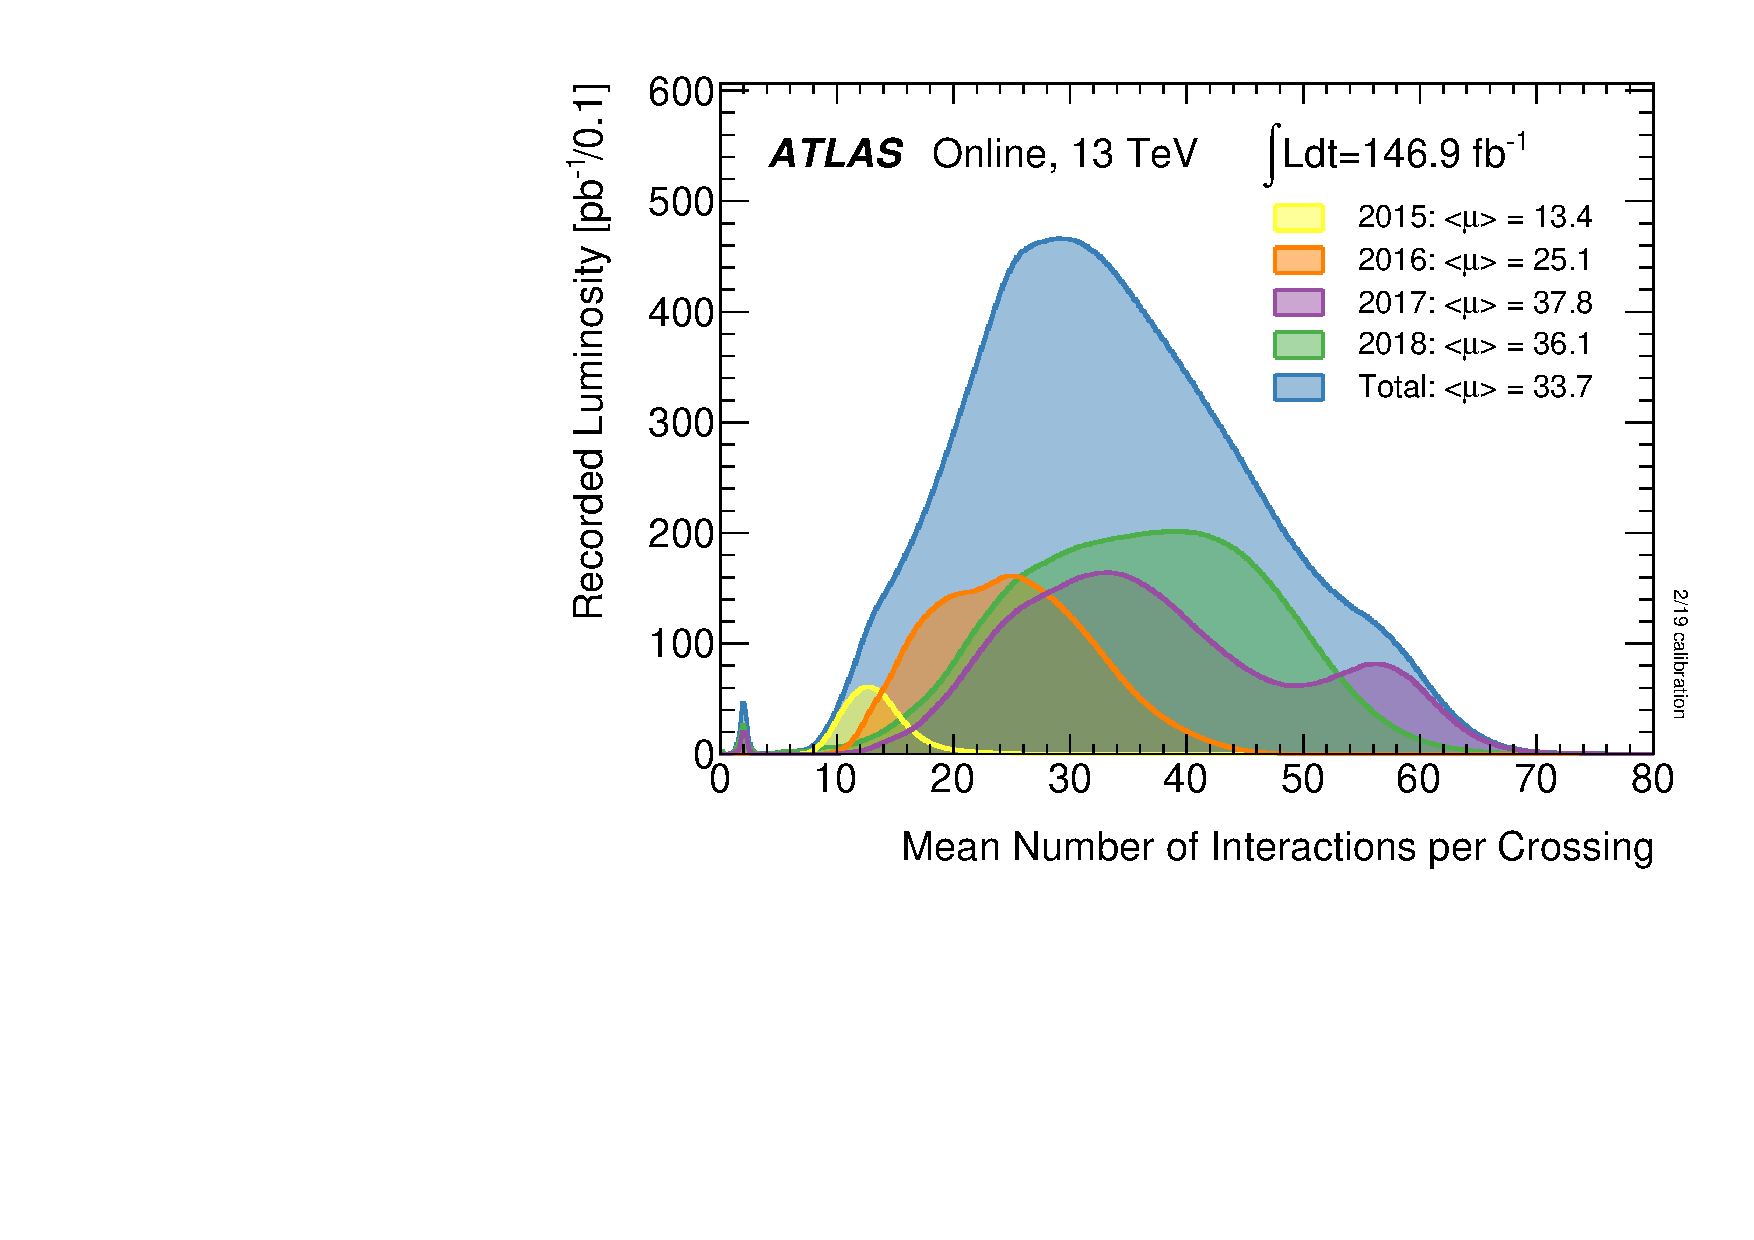
\includegraphics[width=0.7\textwidth]{mu_2015_2018}
\end{center}
\caption{
Shown is the luminosity-weighted distribution of the mean number of interactions per crossing for the 2015-2018 pp collision data at 13 TeV centre-of-mass energy.
All data recorded by ATLAS during stable beams is shown, and the integrated luminosity and the mean mu value are given in the figure. © 2019 CERN
}
\label{fig:mu_per_year}
\end{figure}

\subsection{Backgrounds}
The dominant contribution to the background in this search originates from dijet QCD processes and contributes approximately 92-98\% of the total background yield depending on the region under consideration, as shown in Table~\ref{tab:bkg_comp}.
QCD MC samples do not have enough enough events in the high mass region to model this process in the regions of interest, especially given the high background rejection that is achieved with the $V$ and $H$ tagging techniques.
Therefore, the multijet background is estimated from data, in order to avoid problems associated with theoretical mismodelling and low statistics.

Other contributions to the background composition come primarily from \tt and $V$+jets, totaling from 2 to 10\% of the background, depending on the region.
Since the background prediction is fully data-driven, these MC samples are only used for a limited set of studies.
Standard Model VV, VH and $H \rightarrow gg$ contributions are considered negligible.

\subsubsection{QCD}
For studies with simulated QCD events, the nominal MC samples used are generated with \PYTHIA 8.186, with the NNPDF23LO PDF and the ATLAS A14 tune for the underlying event. Events are generated in bins of \pt\ of \akt R=0.6 truth jets, as listed in Table \ref{tab:dijet}.

\begin{table}[!htb]
\begin{scriptsize}
\begin{center}
\begin{tabular}{|c|l|c|c|c|c|r|}
\hline
DSID & Process & Generator & $\sigma\times\text{BR}$ [fb] & $k$-factor & $\epsilon_{\text{filter}}$ & Events \\ \hline
361023 & \makecell{JZ3W \\ $160 < p_{T}^{jet} < 400$~GeV  }  & \PYTHIA v8.186 + EvtGen v1.2.0 & 2.645e+10 & 1.0 & 0.00032012 & 31758000 \\
\hline
361024 & \makecell{JZ4W \\ $400 < p_{T}^{jet} < 800$~GeV  }  & \PYTHIA v8.186 + EvtGen v1.2.0 & 2.546e+08 & 1.0 & 0.00053137 & 31900000 \\
\hline
361025 & \makecell{JZ5W \\ $800 < p_{T}^{jet} < 1300$~GeV }  & \PYTHIA v8.186 + EvtGen v1.2.0 & 4.554e+06 & 1.0 & 0.00092395 & 31985000 \\
\hline
361026 & \makecell{JZ6W \\ $1300 < p_{T}^{jet} < 1800$~GeV}  & \PYTHIA v8.186 + EvtGen v1.2.0 & 2.575e+05 & 1.0 & 0.0009427 & 35714400 \\
\hline
361027 & \makecell{JZ7W \\ $1800 < p_{T}^{jet} < 2500$~GeV}  & \PYTHIA v8.186 + EvtGen v1.2.0 & 1.622e+04 & 1.0 & 0.0003928 & 31099500 \\
\hline
361028 & \makecell{JZ8W \\ $2500 < p_{T}^{jet} < 3200$~GeV}  & \PYTHIA v8.186 + EvtGen v1.2.0 & 6.250e+02 & 1.0 & 0.010176 & 31986000 \\
\hline
361029 & \makecell{JZ9W \\ $3200 < p_{T}^{jet} < 3900$~GeV}  & \PYTHIA v8.186 + EvtGen v1.2.0 & 1.964e+01 & 1.0 & 0.012077 & 28507000 \\
\hline
361030 & \makecell{JZ10W \\ $3900 < p_{T}^{jet} < 4600$~GeV}  & \PYTHIA v8.186 + EvtGen v1.2.0 & 1.196e+00 & 1.0 & 0.0059083 & 29973000 \\
\hline
361031 & \makecell{JZ11W \\ $4600 < p_{T}^{jet} < 5300$~GeV}  & \PYTHIA v8.186 + EvtGen v1.2.0 & 4.226e-02 & 1.0 & 0.0026761 & 31941000 \\
\hline
361032 & \makecell{JZ12W \\ $p_{T}^{jet} > 5300$~GeV       }  & \PYTHIA v8.186 + EvtGen v1.2.0 & 1.037e-03 & 1.0 & 0.00042592 & 31635600 \\
\hline
\end{tabular}
\caption{Nominal QCD weighted (JZXW) simulated samples used in the analysis. The dataset ID, MC generator, production cross-sections, $k$-factor, filter efficiency and total number of generated events are shown.}
\label{tab:dijet}
\end{center}
\end{scriptsize}
\end{table}

\subsubsection{$V$+jets}
The $W$+jets and $Z$+jets events are generated with \SHERPA 2.1.1 \cite{Gleisberg:2008ta} interfaced with the CT10 PDF set \cite{Gao:2013xoa}. Matrix elements of up to 4 extra partons are calculated at next-to-leading order in $\alpha_S$. Only the hadronic decays of the $W$ and $Z$ are included. The samples are split by boson \pt, as listed in Table \ref{tab:vjets}.

% Updated June 2019
\begin{table}[!htb]
\begin{scriptsize}
\begin{center}
\begin{tabular}{|c|l|c|c|c|c|r|}
    \hline
    DSID & Process & Generator & $\sigma\times\text{BR}$ [fb] & $k$-factor & $\epsilon_{\text{filter}}$ & Events \\ \hline
    304307 & \makecell{$W \rightarrow q \bar{q}^\prime$ + 0,1,2,3,4 partons \\ $280 < p_{T}^{W} < 500$~GeV} & \SHERPA v2.1.1 & 2.949e+04 & 1.0 & 1.0 & 490000 \\
    \hline
    304308 & \makecell{$W \rightarrow q \bar{q}^\prime$ + 0,1,2,3,4 partons \\ $500 < p_{T}^{W} < 1000$~GeV} & \SHERPA v2.1.1 & 2.164e+03 & 1.0 & 1.0 & 170000 \\
    \hline
    304309 & \makecell{$W \rightarrow q \bar{q}^\prime$ + 0,1,2,3,4 partons \\ $p_{T}^{W} > 1000$~GeV}       & \SHERPA v2.1.1 & 4.609e+01 & 1.0 & 1.0 & 115000 \\
    \hline
    304707 & \makecell{$Z \rightarrow q \bar{q}$ + 0,1,2,3,4 partons \\ $280 < p_{T}^{Z} < 500$~GeV}  & \SHERPA v2.1.1 & 1.262e+04 & 1.0 & 1.0 & 250000 \\
    \hline
    304708 & \makecell{$Z \rightarrow q \bar{q}$ + 0,1,2,3,4 partons \\ $500 < p_{T}^{Z} < 1000$~GeV} & \SHERPA v2.1.1 & 9.027e+02 & 1.0 & 1.0 & 144000 \\
    \hline
    304709 & \makecell{$Z \rightarrow q \bar{q}$ + 0,1,2,3,4 partons \\ $p_{T}^{Z} > 1000$~GeV}       & \SHERPA v2.1.1 & 1.823e+01 & 1.0 & 1.0 & 90000 \\
    \hline
\end{tabular}
\caption{
    $W$+jets and $Z$+jets samples used in the analysis. The dataset ID, MC generator, production cross-sections,
    $k$-factor, filter efficiency and total number of generated events are shown.
}
\label{tab:vjets}
\end{center}
\end{scriptsize}
\end{table}

\subsubsection{t$\bar{t}$}
%TODO: tree level feynman diagrams

The \tt samples are generated with \textsc{Powheg-Box} v2 \cite{Frixione:2002ik} with the NNPDF30 PDF, interfaced with \PYTHIA 8 with NNPDF23 PDF and \textsc{A14} tune for parton shower.
\textsc{EvtGen} v1.2.0 \cite{Lange:2001uf} is used for properties of bottom and charm hadron decays. In order to keep statistical fluctuations small across the dijet mass spectrum, additional \tt samples are used which are generated in slices of \tt invariant mass, starting from 1.1 TeV. Double-counting is avoided by explicitly cutting out events in the inclusive sample that have a \tt mass greater than 1.1 TeV.
The samples are listed in Tables \ref{tab:tt} and \ref{tab:ttSliced}. The cross-section of the \tt process is normalized to NNLO+NNLL in QCD, as calculated by \textsc{Top++} 2.0 \cite{Czakon:2011xx}. The \POWHEG \textsc{hdamp} parameter \cite{ATL-PHYS-PUB-2014-005} is set to 1.5 times the top mass.

% Updated June 2019
\begin{table}[!htb]
\begin{scriptsize}
\begin{center}
\begin{tabular}{|c|l|c|c|c|c|r|}
    \hline
    DSID & Process & Generator & $\sigma\times\text{BR}$ [fb] & $k$-factor & $\epsilon_{\text{filter}}$ & Events \\ \hline
    410471 & all-hadronic \tt & \makecell{\POWHEG + \PYTHIA v8.230 \\ + EvtGen v1.6.0} & 7.298e+05 & 1.0 & 0.45623 & 109738000 \\
    \hline
\end{tabular}
\caption{The \tt inclusive sample used in the analysis. The dataset ID, MC generator, production cross-sections,
$k$-factor, filter efficiency and total number of generated events are shown.}
\label{tab:tt}
\end{center}
\end{scriptsize}
\end{table}

% Updated June 2019
\begin{table}[!htb]
\begin{scriptsize}
\begin{center}
\begin{tabular}{|c|l|c|c|c|c|r|}
\hline
DSID & Process & Generator & $\sigma\times\text{BR}$ [fb] & $k$-factor & $\epsilon_{\text{filter}}$ & Events \\ \hline
410284 & \makecell{all-hadronic \tt \\ $1.1 < m_{t\bar{t}} < 1.3$~TeV} & \makecell{\POWHEG + \PYTHIA v8.230 \\ + EvtGen v1.6.0} & 7.298e+05 & 1.0 & 0.0038853 & 2045000 \\
\hline
410285 & \makecell{all-hadronic \tt \\ $1.3 < m_{t\bar{t}} < 1.5$~TeV} & \makecell{\POWHEG + \PYTHIA v8.230 \\ + EvtGen v1.6.0} & 7.298e+05 & 1.0 & 0.0015782 & 777000 \\
\hline
410286 & \makecell{all-hadronic \tt \\ $1.5 < m_{t\bar{t}} < 1.7$~TeV} & \makecell{\POWHEG + \PYTHIA v8.230 \\ + EvtGen v1.6.0} & 7.298e+05 & 1.0 & 0.00069112 & 389300 \\
\hline
410287 & \makecell{all-hadronic \tt \\ $1.7 < m_{t\bar{t}} < 2.0$~TeV} & \makecell{\POWHEG + \PYTHIA v8.230 \\ + EvtGen v1.6.0} & 7.298e+05 & 1.0 & 0.00042428 & 335740 \\
\hline
410288 & \makecell{all-hadronic \tt \\ $2.0 < m_{t\bar{t}} < 14$~TeV } & \makecell{\POWHEG + \PYTHIA v8.230 \\ + EvtGen v1.6.0} & 7.298e+05 & 1.0 & 0.00023803 & 187700 \\
\hline
\end{tabular}
\caption{Additional \tt samples used in the analysis. The dataset ID, MC generator, production cross-sections,
$k$-factor, filter efficiency and total number of generated events are shown.}
\label{tab:ttSliced}
\end{center}
\end{scriptsize}
\end{table}

\section{Object Selection}
%TODO: cite relevant sections of Ch3
\label{sec:objects}

\subsection{Large Radius Jets}
\label{sec:tccjets}
In order to identify and reconstruct potential vector boson and Higgs boson candidates, large radius parameter ("large-$R$") jets are used.
In prior years the de facto jet algorithm in this circumstance was the \akt algorithm with a radius parameter of $R=1.0$ utilizing locally weighted topological cell clusters (LCTopo)~\cite{PERF-2014-07} for constituents.
A new jet type of jet constituent known as Track-CaloCluster (TCC) has been developed \cite{ATL-PHYS-PUB-2017-015} which combines calorimeter and tracking data in such a way as to leverage the most performant aspects of both.
In practice TCC jets exploit the superior spatial resolution of the tracker and the energy measurement of the calorimeter.
This approach is particularly beneficial for recovering angular information from highly boosted jet constituents that would otherwise merge and be lost due to the resolution limitations when using the calorimeter alone.
A comparison of jet mass and \d2 resolution is shown in Figure ~\ref{fig:tcc_lctopo_res}.
For these reasons TCC jets are used in this analysis rather than LCTopo.
Refer to Section~\ref{sec:jet_constituents} for more details.

Pileup dependence is significantly negated by jet trimming ~\cite{Krohn:2009th} with parameters $f_{\mathrm{cut}} = 0.05$ and $R_{\mathrm{sub}} = 0.2$, as described in Section~\ref{sec:jet_substructure}.
A Monte Carlo based particle-level calibration is applied to the jets used in this analysis, which corrects on average the reconstructed mass and \pt\ of the jets to their true values, as described in Section~\ref{sec:jet_calibration}.

\begin{figure}[htbp!]
\begin{center}
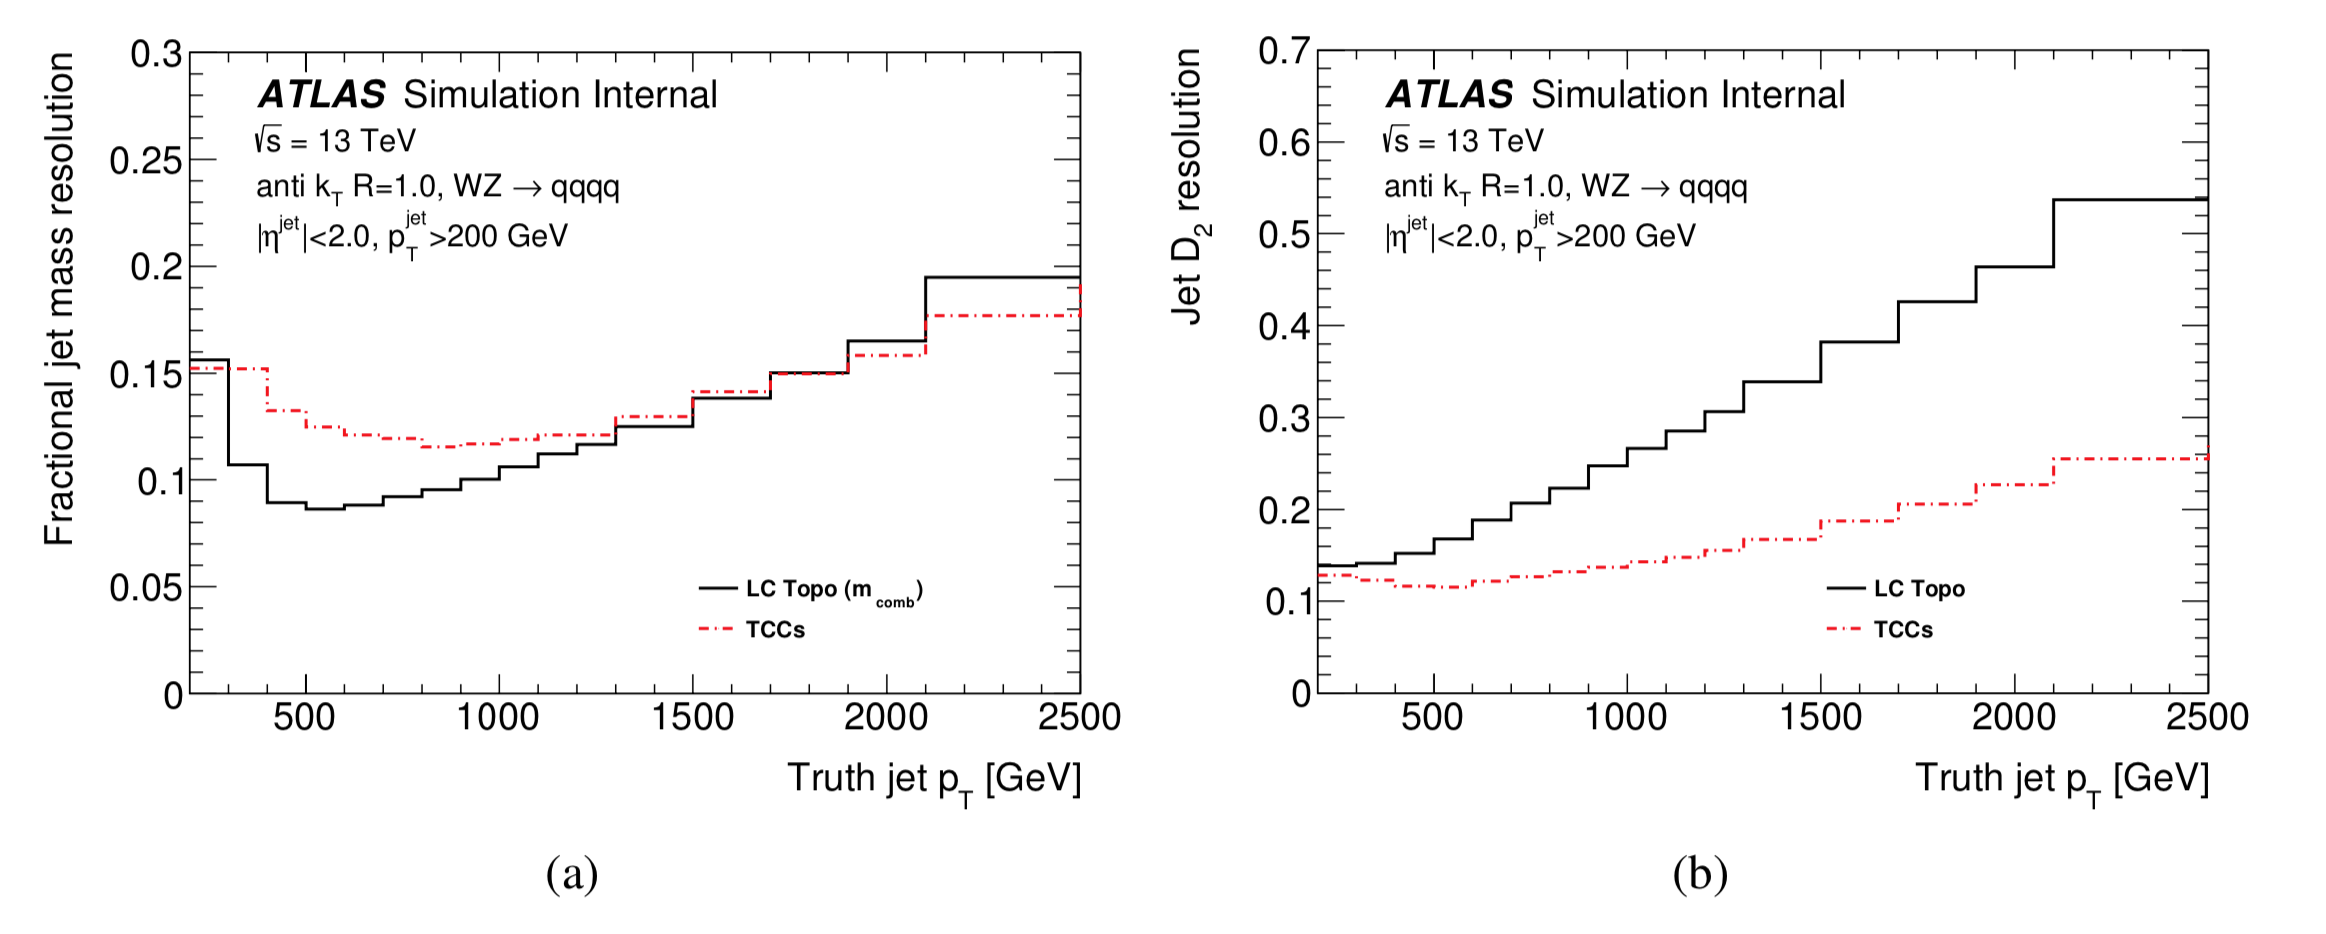
\includegraphics[width=\textwidth]{TCC_LCTopo_Mass_D2_resolution.png}
\end{center}
\caption{A comparison of the fractional jet (a) mass and (b) \d2 resolution for LCTopo (solid black lines) and TCC (dashed red lines) as a function of truth jet \pt. © CERN}
\label{fig:tcc_lctopo_res}
\end{figure}

%\TODO{reference trigger section}
All large-R jets are required to have a $p_T$ of at least 200 GeV in order to ensure they fall within the region of phase space where the jet calibration is well understood.
Furthermore, each large-R jet is required to have $|\eta|<2.0$ to ensure that the track-jets associated with it are contained within the ID acceptance.
The leading large-R jet must also have a $p_T$ greater than 500 GeV, ensuring that the large-R jet is in the trigger efficiency plateau for triggers used in 2015, 2016, 2017, and 2018 datasets.
The large-R jet reconstruction, calibration, and selection parameters are summarized in Table ~\ref{tab:jet_parameters}.

\begin{table}[!htb]
%\begin{scriptsize}
\begin{center}
\begin{tabular}{|c|c|c|c|}
\hline
Parameter & Value \\
\hline
Algorithm & anti-$k_T$ \\
Radius & 1.0 \\
Constituent Type & TrackCaloClusters \\
Grooming Algorithm & Trimming $(f_{\mathrm{cut}} = 0.05, R_{\mathrm{trim}} = 0.2)$ \\
Calibration Sequence & $\eta$ + JES + JMS \\
\pt\ Cut & $> 500$ GeV (leading), $> 200$ GeV (sub-leading) \\
$\left| \eta \right|$ Cut & $< 2.0$ \\
\hline
\end{tabular}
\caption{Summary of jet reconstruction and selection parameters for this analysis.}
\label{tab:jet_parameters}
\end{center}
%\end{scriptsize}
\end{table}

\subsection{Track-jets}
\label{sec:track_jets}
%TODO: Explain VR jet algorithm in jets chapter and reference here
%TODO: Make picking out b-quarks from Higgs decay the obvious purpose of these jets
Track-jets are built by clustering Inner Detector tracks using the \akt algorithm.
All tracks used are required to be associated with the primary vertex of the event, defined as the vertex with the largest $\sum p_T^2$.
The selected tracks are required to have $p_T$ greater than 500 MeV and pass the ``Loose'' tracking quality cuts.
In this analysis the variable-radius track jet collection is used, where the radius parameter is a function of the jet $p_{T}$ as $R=\rho/p_{T}$.
The parameter $\rho$ is set to 30 GeV, and the minimum and maximum values for the radius are set to 0.02 and 0.4, respectively \cite{ATL-PHYS-PUB-2017-010}.

When compared to calorimeter jets, the smaller $R$ parameters in track-jets coupled with the fact that tracks have better angular resolution than calorimeter clusters, mean that the decay products of highly boosted heavy objects can still be resolved.
After clustering, track-jets are then associated to the large-R calorimeter jets via ghost-association \cite{Cacciari:2008gn}, a procedure that treats them as four-vectors of infinitesimal magnitude during the jet reconstruction and assigns them to the jet with which they are clustered.

A $b$-tagging algorithm is used to identify track-jets which are likely to contain $b$-hadrons from the Higgs boson decay. The MV2 algorithms exploit the relatively long lifetime and large mass of $b$-hadrons with respect to lighter hadrons, as well as the kinematics of the charged particle tracks.

Optimization studies were performed in order to determine the best $b$-tagging algorithm and working point for this search.
The MV2c10 algorithm is used with the 77\% fixed efficiency working point, as measured from $b$ jets in \tt events, which corresponds to a background rejection of 1/5 for $c$ jets and 1/112 for light jets.

\subsection{Leptons}
\label{sec:leptons}
% Explain purpose of lepton veto
Based on the lepton veto applied in the ATLAS $Z' \rightarrow ZH\rightarrow \nu\bar{\nu} b\bar{b}$ analysis, events with at least one loose lepton are rejected.
Loose muons are required to have $p_{T}>7$~GeV and fall in the central region of the detector ($|\eta|<2.5$). They are identified with the "loose" quality working point. Track quality requirements are applied such that $|d_{0}/\sigma(d_{0})|<3$ and $|z_{0}\sin\theta|<0.5$~mm, where $d_{0}$ and $z_{0}$ are the transverse and longitudinal track impact parameters. Loose electrons are also required to have $p_{T}>7$~GeV, with a pseudorapidity requirement such that $|\eta|<2.47$. As with muons, requirements on the transverse and longitudinal impact parameters of the associated tracks are made. In terms of isolation, both loose electrons and loose muons are required to be "LooseTrackOnly", where a cone with radius $r(p_{T}^{\ell})=\min(0.2,10~\text{GeV}/p_{T}^{\ell})$ (0.3 for muons) is constructed around each lepton and for which the $p_{T}$-sum of all tracks with $p_{T}>500$~MeV defines the isolation $I_\ell$. A cut on $I_\ell/p_{T}^{\ell}<I_{0}$ is imposed, and $I_{0}$ is such that a flat efficiency of 99\% as a function of $p_{T}$ and $\eta$ is obtained for lepton candidates in $Z\rightarrow \ell \ell$ events.

\section{Event Selection}
\label{sec:selection}

\subsection{Pre-Selection}
\label{subsec:presel}

\subsubsection{EXOT3 Derivation: xAOD $\rightarrow$ DxAOD}
\label{subsec:exot3}

All data and MC samples are initially produced in xAOD format.
In order to reduce the file size of these samples, the derivation framework is used to remove both objects and entire events of no interest to the analysis.
The EXOT3 derivation is used\footnote{\path{https://gitlab.cern.ch/atlas/athena/blob/21.2/PhysicsAnalysis/DerivationFramework/DerivationFrameworkExotics/share/EXOT3.py}}.
Beyond reducing file size, the derivation is also responsible for the production of nonstandard jet collections, such as the fat jet collections needed for this analysis.

A \textit{slimming} procedure is applied in order to remove all but the essential variables for calibration of the following objects:
\begin{itemize}
    \item \path{Electrons}
    \item \path{Muons}
    \item \path{MET_Reference_AntiKt4LCTopo}
    \item \path{InDetTrackParticles}
    \item \path{PrimaryVertices}
    \item \path{AntiKt4EMTopoJets}
\end{itemize}

A \textit{thinning} procedure is applied in order to remove some objects based on the following criteria:

\begin{itemize}
    \item \path{InDetTrackParticles}: must be associated with
    \begin{itemize}
        \item An electron
        \item A muon
        \item An AntiKt10LCTopoJet with \pt > 150 GeV and $|\eta| < 2.8$.
        \item An AntiKt10TrackCaloCluster jet
    \end{itemize}
    \item \path{LCOriginTopoClusters}: must be associated with
    \begin{itemize}
        \item An AntiKt10LCTopoJet with \pt > 150 GeV and $|\eta| < 2.8$.
        \item An AntiKt10TrackCaloCluster jet
    \end{itemize}
\end{itemize}

A \textit{skimming} procedure is also applied to remove entire events from the xAOD with the following criteria:
\begin{itemize}

    \item Topological large-R jet selection
        \begin{itemize}
            \item >2 calibrated offline AntiKt10LCTopoTrimmedPtFrac5SmallR20Jets jets with
                \begin{itemize}
                    \item \pt\ > 100 GeV
                    \item $|\eta|$ < 2.8
                    \item $m > 30$ GeV for jets with $\pt < 1.0\ TeV$
                \end{itemize}
        \end{itemize}
    \item Events must be required to pass one of a long list of jet-related ATLAS triggers.
\end{itemize}

In total the combined EXOT3 skimming, thinning, and slimming reduces the file size to ~2\% of the original size for data.

\subsubsection{Event Cleaning}
\label{subsec:evtclean}
%TODO: add footnotes explaining beam halo and cosmic rays
%TODO: mention percent of events removed by event cleaning
Non-collision backgrounds originating from calorimeter noise, beam halo interactions or cosmic rays can lead to spurious calorimeter signals and the reconstruction of "bad" jets. This effect can be suppressed by applying a standard jet cleaning procedure, which has been developed for 2015 data to reject jets based on their shape and timing information \cite{jetSelection} . Events are rejected if they contain at least one small radius jet (anti-$k_T$, with $R=0.4$) classified as ``bad-loose'' by the aforementioned jet cleaning criteria.
Additional vetos are applied to reject events where Tile or LAr calorimeter errors occur, as well as single event upsets in the SCT. These cuts are applied by accessing information via special flags recorded by each subdetector on a per-event basis. Incomplete events are also flagged and rejected by inspecting similar flags.
Events are also required to have at least one primary vertex with at least two tracks.

Due to the nature of the VR track jet reconstruction it is possible for one VR track jet $(i)$ to be fully contained within another $(j)$ in terms of their angular separation.
This overlap condition can be expressed with the following inequality:
\begin{equation}
    \Delta R(i,j) < \min(R_i, R_j)
\end{equation}
Any VR track jets matching this criterion are removed from consideration.
This prevents the utilization of track jets with an ambiguous association of tracks for $b$-tagging, because in these cases it is likely that the $b$-tagging calibration scale factors are not correct.
See Figure~\ref{fig:vr_contain} for an illustration of this phenomenon.

\begin{figure}[htbp!]
    \begin{center}
        \subfloat[]{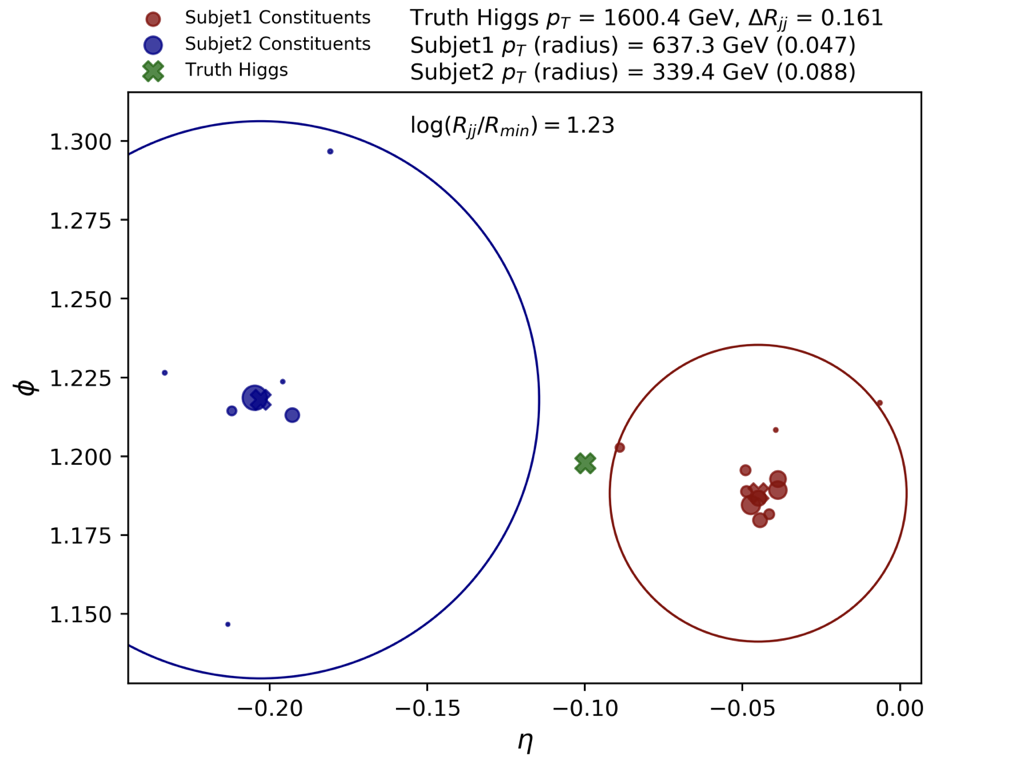
\includegraphics[width=.75\linewidth]{vr_containment_good.png}}\\
        \subfloat[]{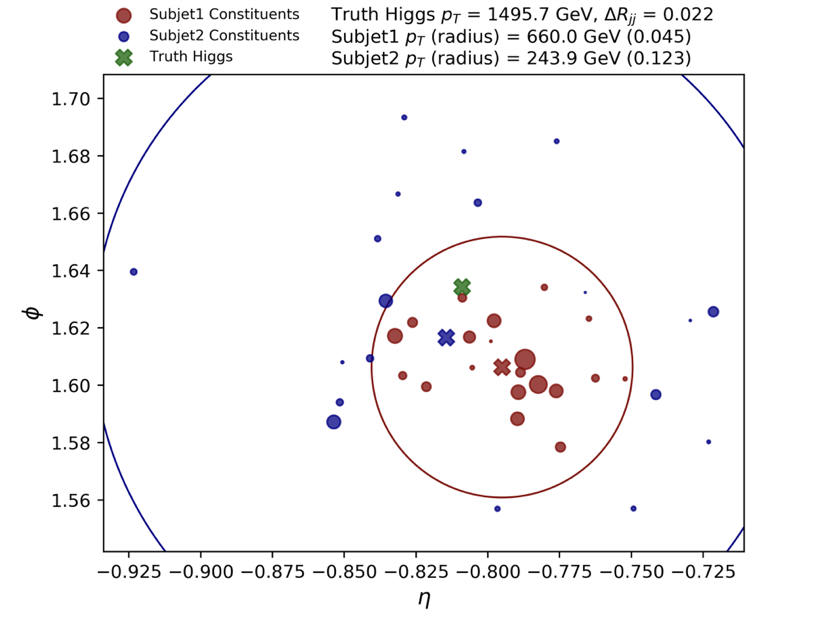
\includegraphics[width=.75\linewidth]{vr_containment_bad.png}}
    \end{center}
    \caption{ $\eta-\phi$ distribution (from simulation) of constituents of the two leading \pt\ VR track jets ghost associated to a truth large-R Higgs jet.
        Two illustrative cases are shown: (a) clean separation of track jet constituents and (b) pathological overlap.
        The radii of the filled red/blue circles are proportional to $\log{\pt}$ of the corresponding track jet constituent.
    }
    \label{fig:vr_contain}
\end{figure}

\subsection{Trigger Requirements}
\label{subsec:trig}
%2015: HLT_j360_a10_lcw_sub_L1J100
%2016: HLT_j420_a10r_L1J100
%2017/2018: HLT_j460_a10t_lcw_jes_L1J100

For the analysis of the 2015 dataset, a high $p_T$, unprescaled large-$R$ jet trigger is used to trigger events: HLT\_j360\_a10\_lcw\_sub\_L1J100. During the 2016 data taking, given the increase in instantaneous luminosity, the trigger with a higher threshold is used: HLT\_j420\_a10r\_L1J100. For the 2017 and 2018 datasets an even higher threshold is used: HLT\_j460\_a10t\_lcw\_jes\_L1J100. The 2015/2016 triggers listed above fire on the untrimmed jet $p_T$, while the 2017/2018 trigger fires on the trimmed jet $p_T$ and applies a subsequent jet energy scale calibration.

For all datasets the offline selection is chosen to produce nearly 100\% efficiency. No trigger-related scale factors are needed in MC simulation to match the efficiency obtained in data.
The efficiency of the relevant triggers as a function of leading large-R jet $\pt$ are shown in Figure~\ref{fig:trigeffturnon}.

\begin{figure}[htbp!]
\begin{center}
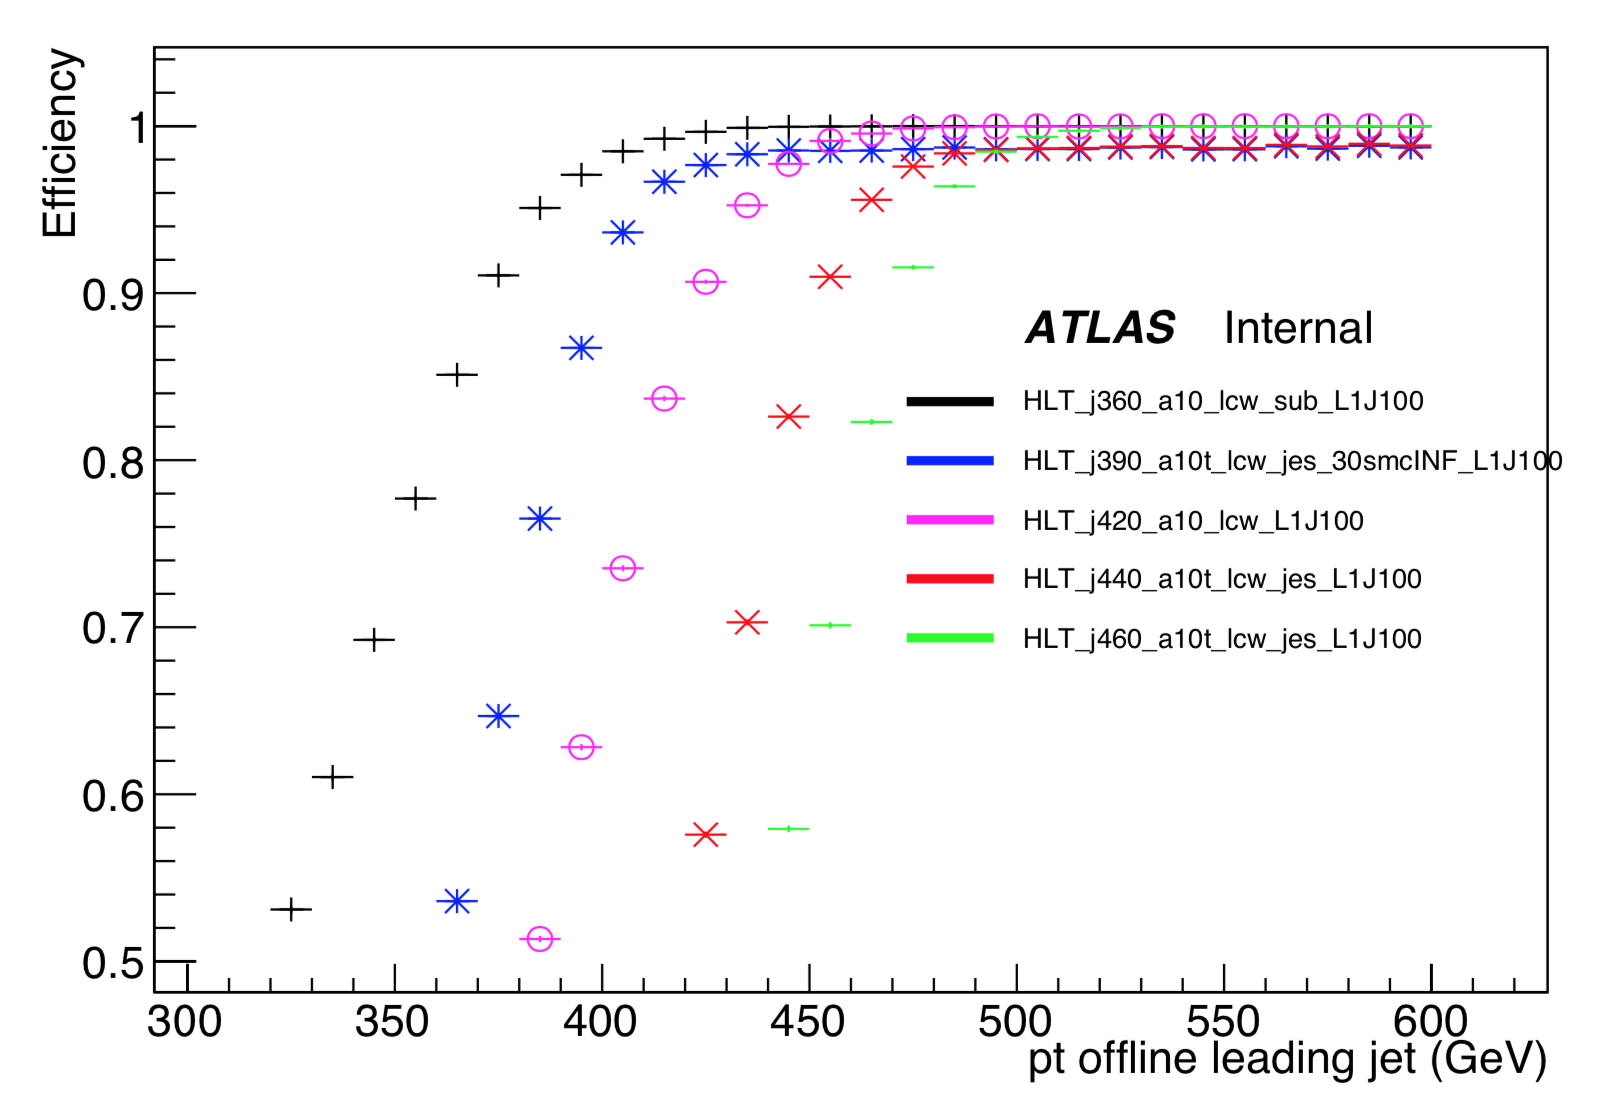
\includegraphics[width=0.49\textwidth]{trigger_eff_vs_pt.png}
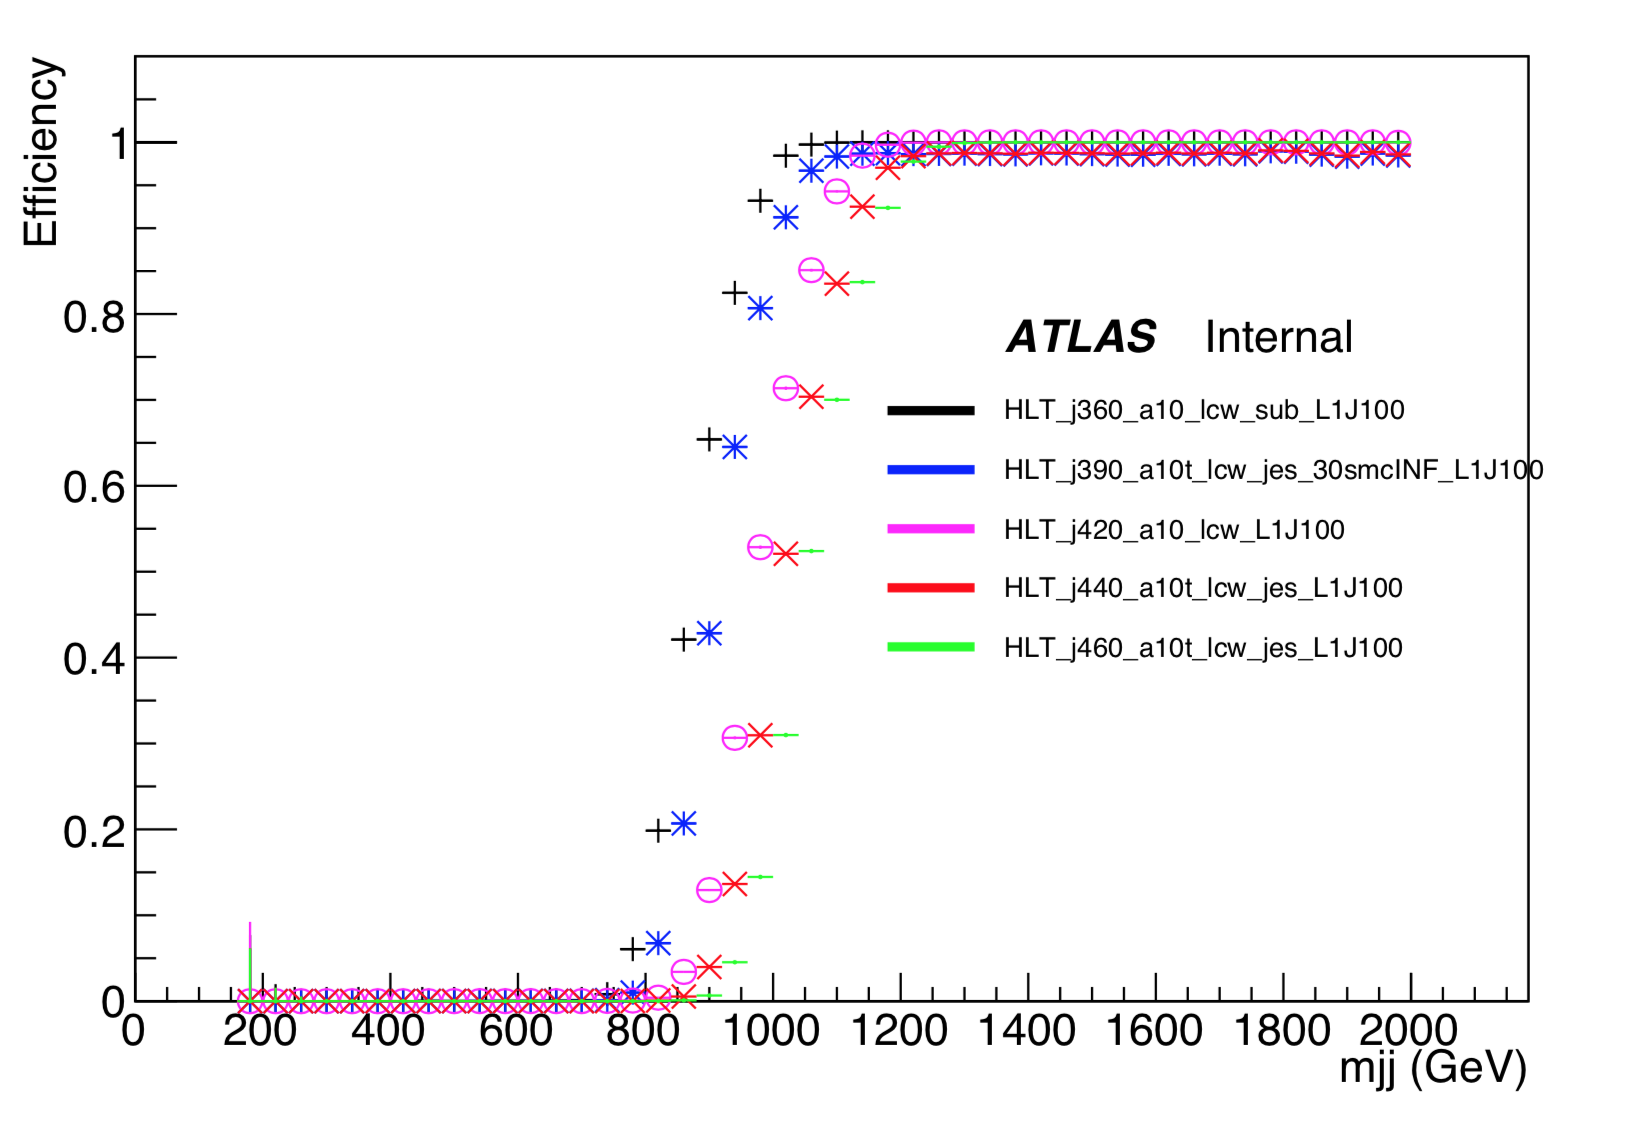
\includegraphics[width=0.49\textwidth]{trigger_eff_vs_mjj.png}
\end{center}
\caption{
    The efficiency of a range of HLT large-R jet triggers as a function of the leading large-R jet $p_T$ (left) and dijet mass (right).
    The dijet mass (right) plot is produced after applying a flat leading jet $p_T$ cut of 500 GeV.
    © CERN
}
\label{fig:trigeffturnon}
\end{figure}

\subsubsection{Jet Selection}
At least two large-$R$ jets are required to be present in the event which pass the kinematic cuts explained in Section \ref{sec:objects}.
In order to ensure full trigger efficiency, a cut of 500 GeV is placed on the leading large-R jet $\pt$ along with a cut on the dijet mass (\mjj > 1.3 TeV).
The two leading jets in the event will correspond to a vector boson and a Higgs boson candidate, the assignment of which is made based on their invariant masses: the heaviest jet is chosen as the Higgs candidate and the lightest as the $W/Z$ candidate.
%Previous studies of alternative methods of H/V candidate assignment have been performed and are documented in a previous support note for this analysis ~\cite{ATL-COM-PHYS-2016-482}.
The remaining $H$ or $W/Z$ specific cuts described below apply to each jet according to this assignment.
Figure \ref{fig:assignment} shows the fraction of events that are correctly matched with this V/H assignment, by checking that the jets chosen for vector and Higgs boson candidates match the truth-level bosons in the signal samples, as a function of the resonance mass.
The truth matching requirement is defined as $\Delta R < 1.0$ between the untrimmed parent of the reconstructed large radius jet and the truth boson.

\begin{figure}[htbp!]
\begin{center}
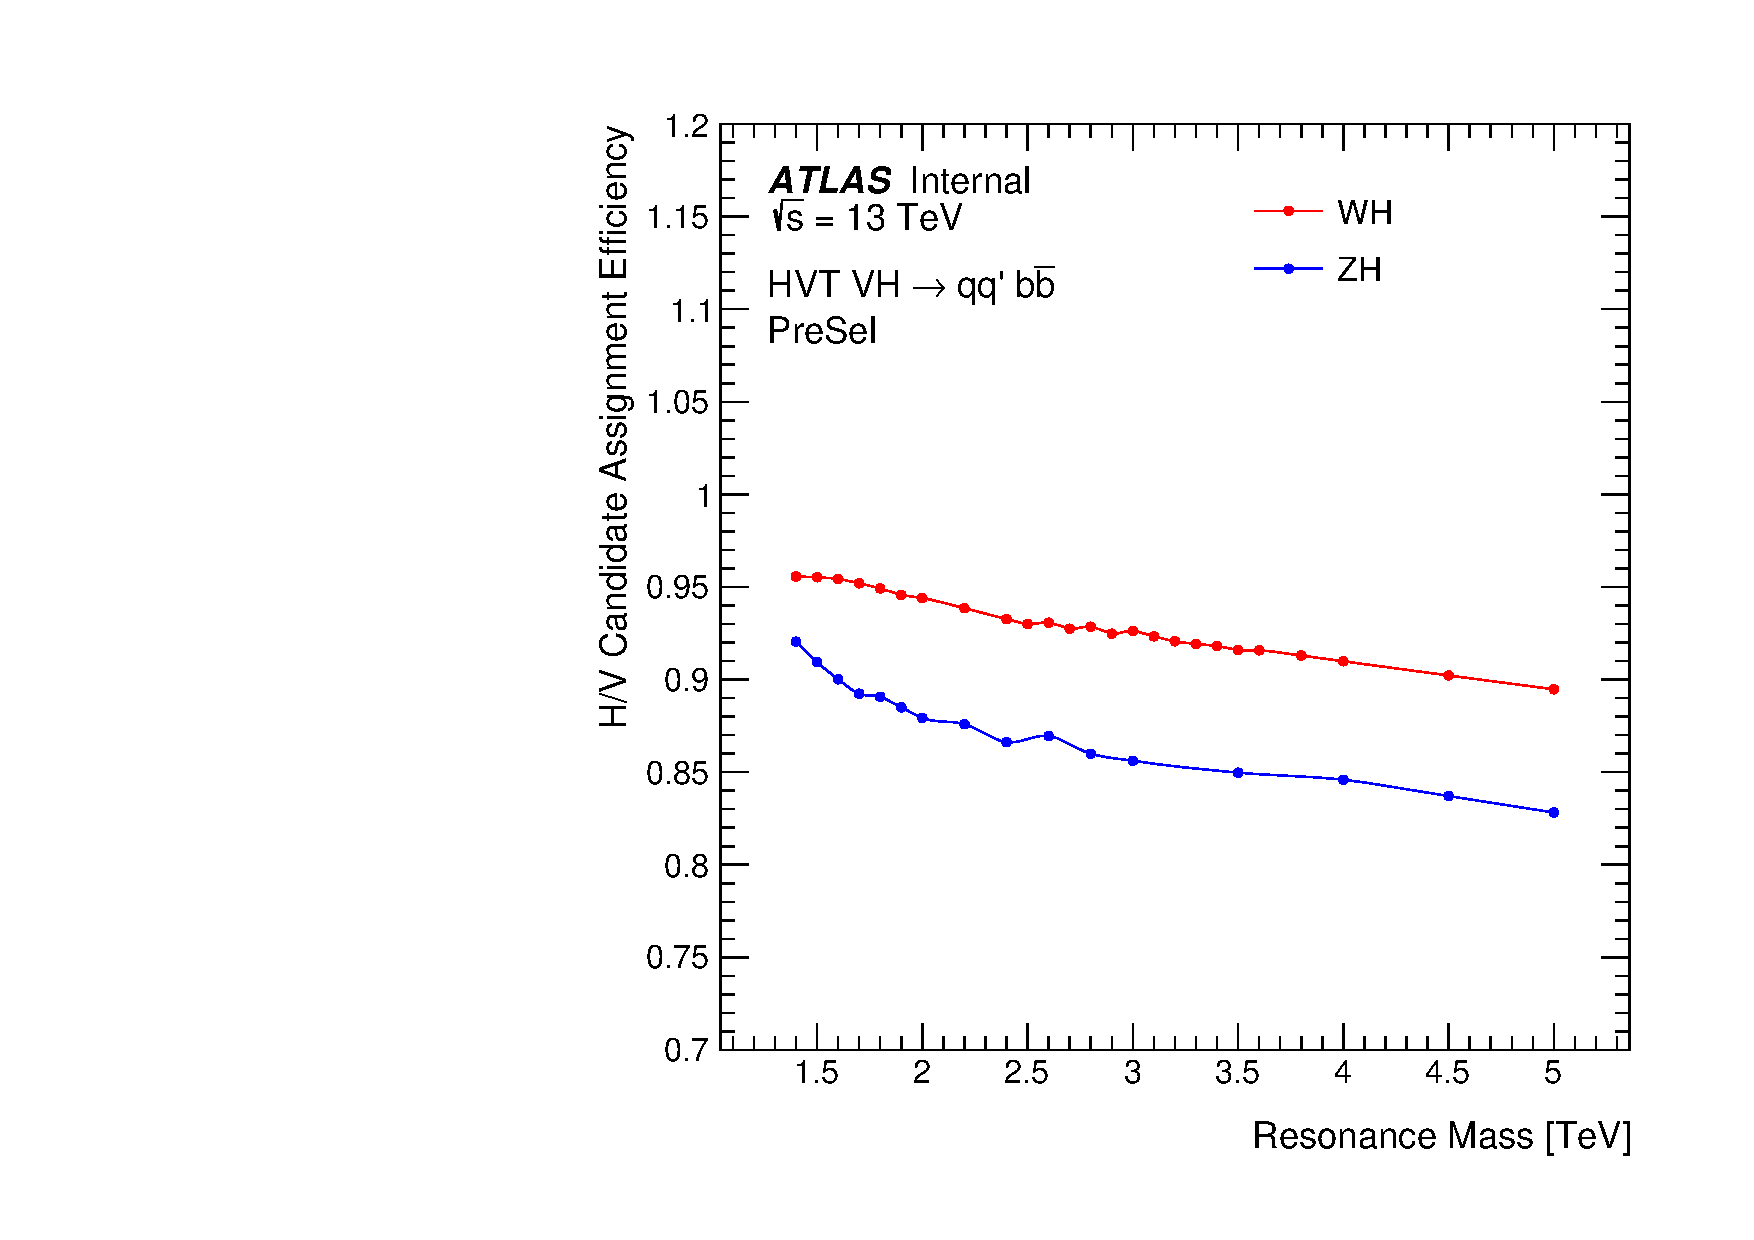
\includegraphics[width=0.49\textwidth]{VHqqbb_HVCandAssignEff_presel.pdf}
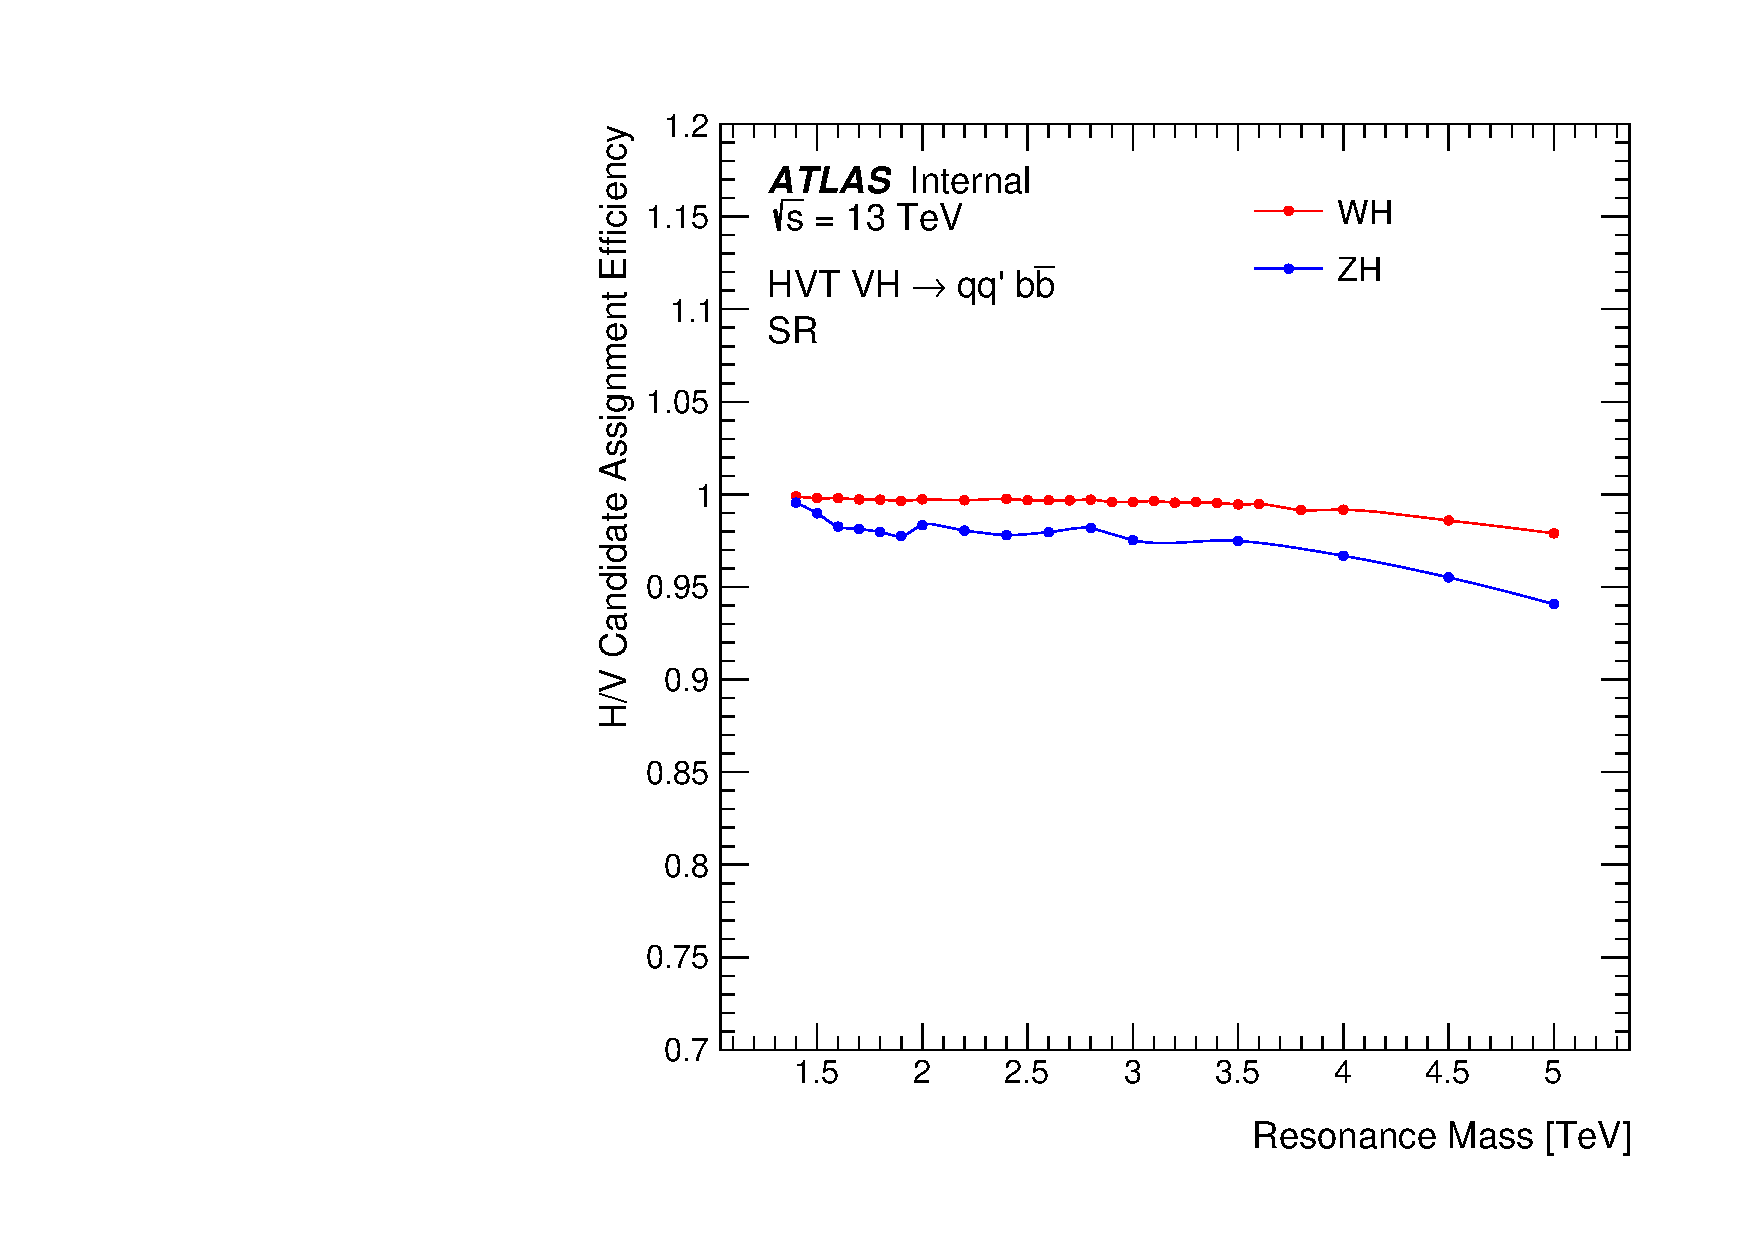
\includegraphics[width=0.49\textwidth]{VHqqbb_HVCandAssignEff_SR.pdf}
\end{center}
\caption{
Fraction of correct V/H assignments for TCC large-R jets based on the V/H assignment criteria described in the text, for $WH$ and $ZH$ signal samples, as a function of the resonance mass.
Loose pre-selection is used on the left while the combined SRWH/SRZH selection is shown on the right.
The difference in efficiency for WH vs. ZH final states is due to the closer proximity of the Higgs and Z boson masses, which produces more overlap between the optimized mass windows (see Figures~\ref{fig:vvjj_wz_tagger_mass_d2_cuts} and~\ref{fig:higgs_tagger_cuts}).
}
\label{fig:assignment}
\end{figure}

\subsubsection{Dijet Mass}
The dijet mass of the $VH$ system, labelled \mvh\ or $m_{\mathrm{VH}}$ in this analysis, is required to be greater than 1.3 TeV in order to ensure full trigger efficiency.
A comparison of simulated background and signal distributions for \mvh\ can be found in Figure~\ref{fig:simple_mc_mVH}.

\begin{figure}[htbp!]
\begin{center}
    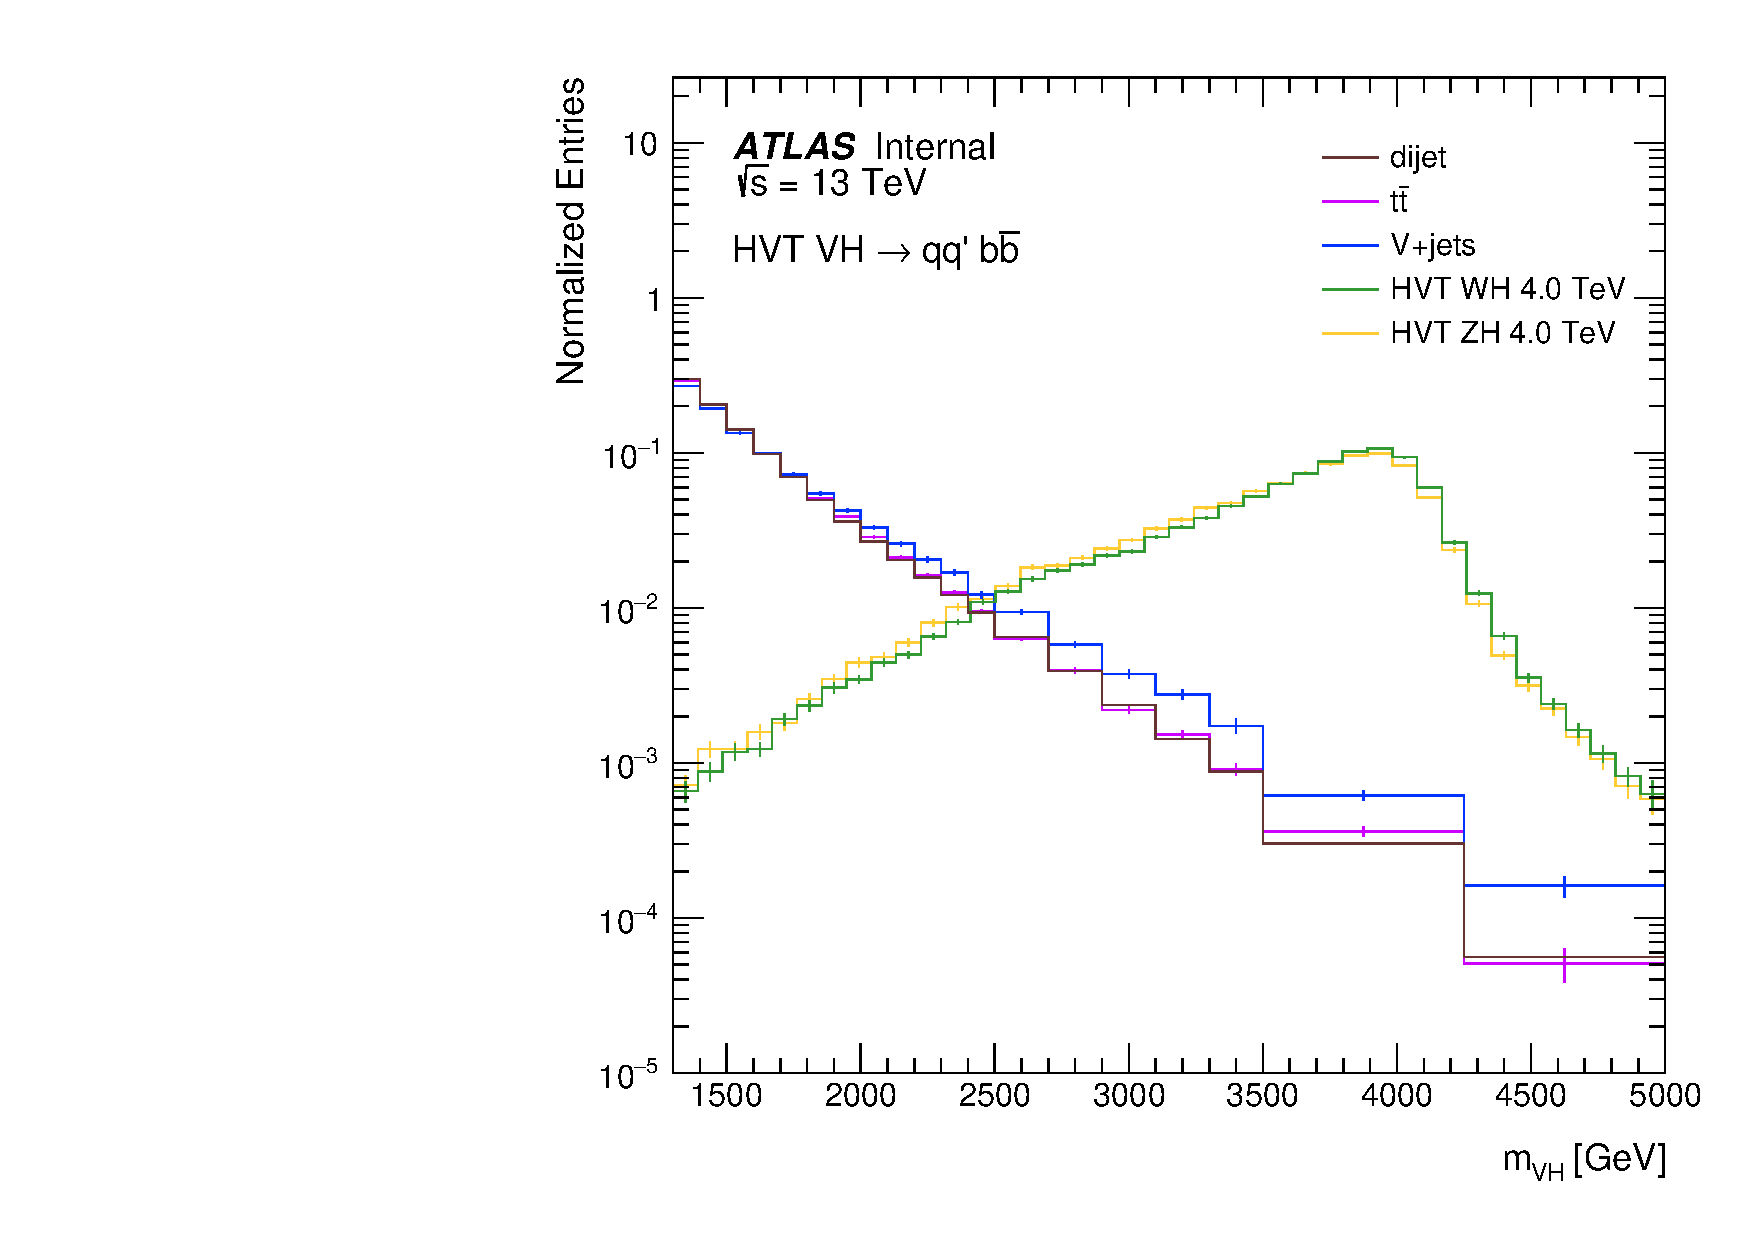
\includegraphics[width=0.49\textwidth]{Ch5_VHqqbb/figures/VHqqbb_SimpleSigBkgMC_mVH.pdf}
\end{center}
\caption{Dijet mass \mvh, as measured in signal and background MC samples, normalized to unity.
Only pre-selection is applied, as described in Section~\ref{subsec:presel}.}
\label{fig:simple_mc_mVH}
\end{figure}

\subsubsection{Rapidity Difference}
%TODO: describe optimization method for the rapidity cut
Due to their exclusive $s$-channel production, signal \wpwh and \zpzh events are expected to be more centrally produced than QCD dijet events, resulting in a rapidity difference (\dy12) between the two leading large-$R$ jets which peaks near 0 (see Figure~\ref{fig:simple_mc_rapidity}).
Leading jets in this analysis are therefore required to have a small rapidity separation. A fixed cut of $|\Delta{y}_{12}|<1.6$ is applied.
%The optimization of this cut is described in~\cite{ATL-COM-PHYS-2016-482}.
A comparison of simulated background and signal distributions for \dy12\ can be found in Figure~\ref{fig:simple_mc_rapidity}.

\begin{figure}[htbp!]
\begin{center}
    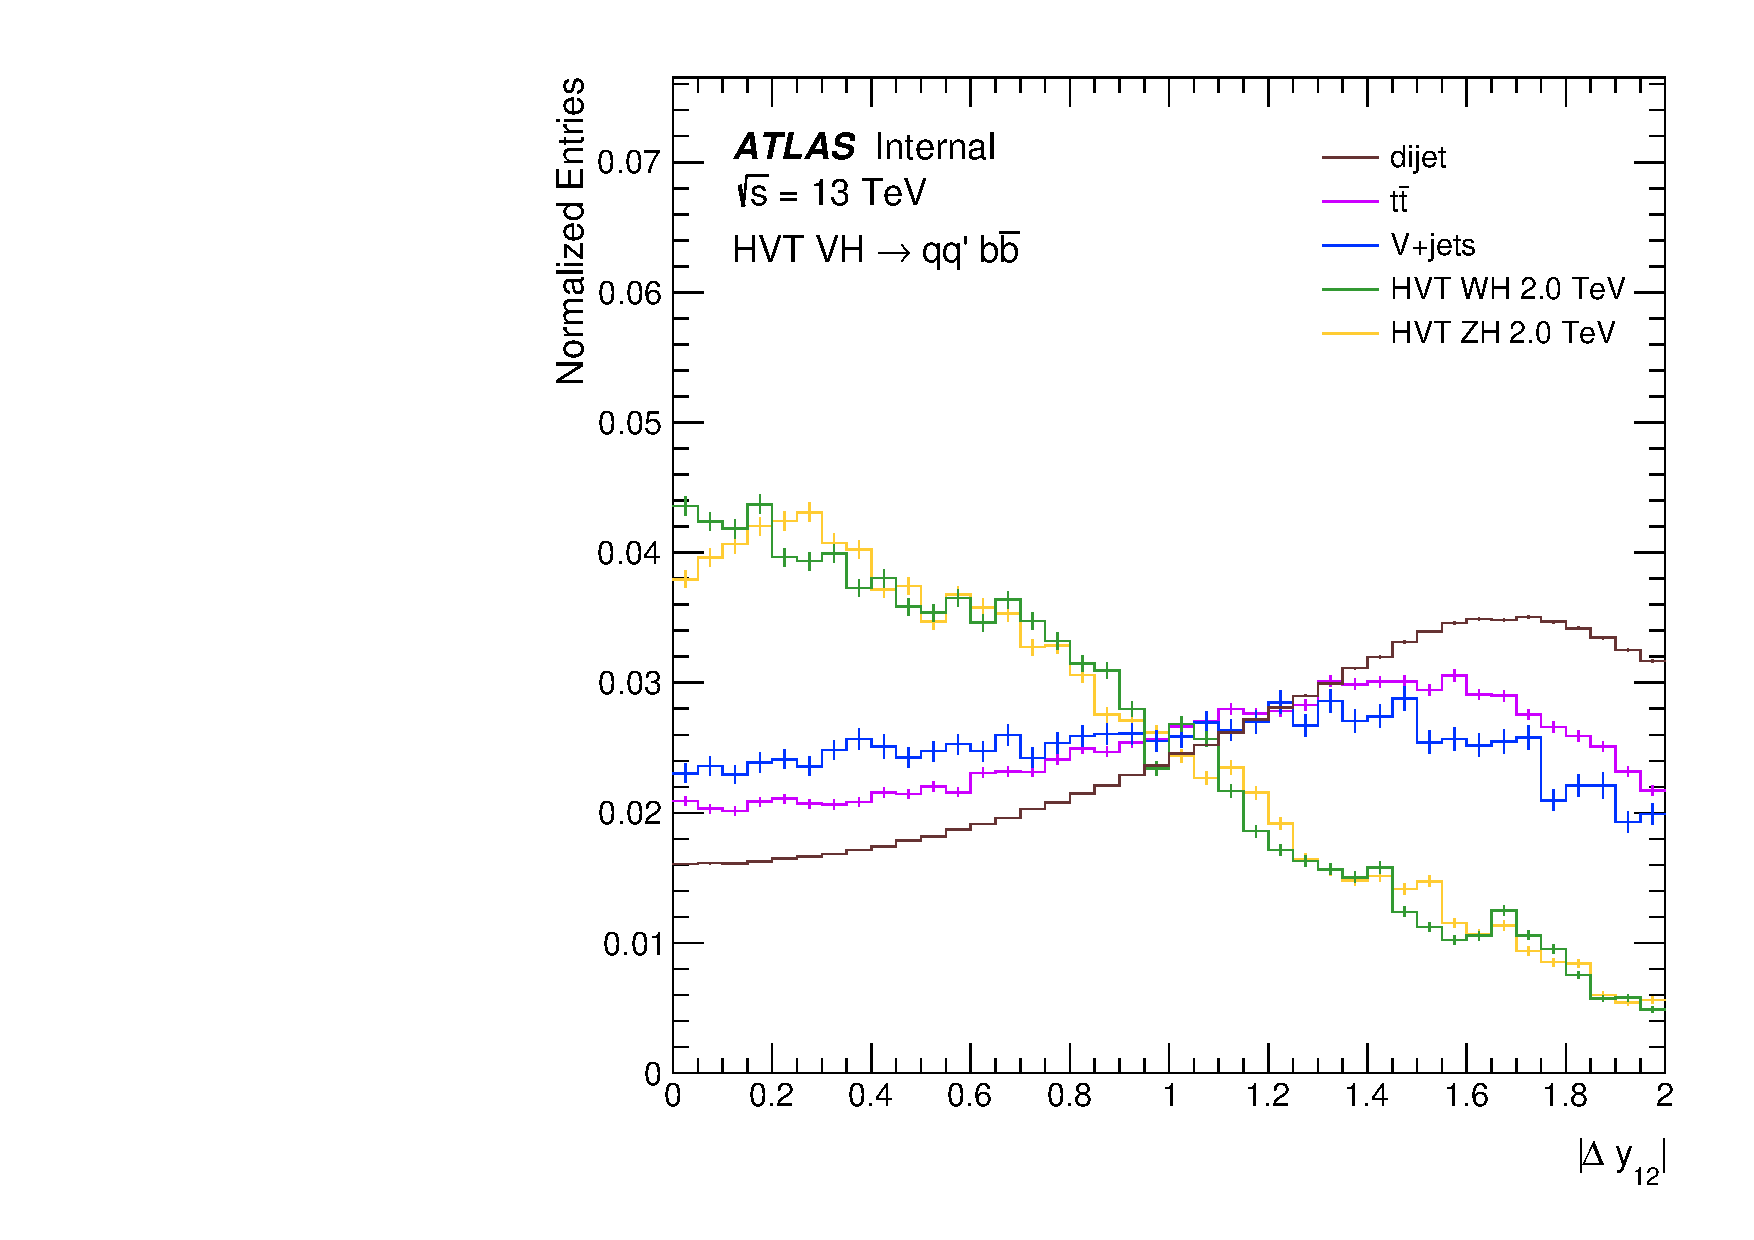
\includegraphics[width=0.49\textwidth]{VHqqbb_SimpleSigBkgMC_dyVH.pdf}
\end{center}
\caption{Distributions of the rapidity difference between the two leading \pt large-$R$ jets, as measured in signal and background MC samples, normalized to unity. Only pre-selection is applied, as described in Section~\ref{subsec:presel}. }
\label{fig:simple_mc_rapidity}
\end{figure}

The sequence of cuts applied and their corresponding efficiencies in data for all elements of the pre-selection data can be found in Table ~\ref{tab:data_cutflow}.

\begin{table}[htbp!]
\normalsize
\centering
\begin{tabular}{c||ccc}
    Selection & Data & Efficiency [\%] & Total Efficiency [\%] \\ \hline
    EXOT3                     & 505568676 & --    & -- \\ \hline
    GRL + EventCleaning       & 483433031 & 95.62 & 95.62 \\ \hline
    Jet Cleaning              & 477623453 & 98.80 & 94.47 \\ \hline
    Trigger                   & 128220751 & 26.85 & 25.36 \\ \hline
    Jet multiplicity          & 128136392 & 99.93 & 25.35 \\ \hline
    Fatjet EtaPtPreSel        & 106779224 & 83.33 & 21.12 \\ \hline
    Lead Jet pT               & 52157511  & 48.85 & 10.32 \\ \hline
    mVH                       & 23981560  & 45.98 & 4.74 \\ \hline
    DeltaY                    & 12497837  & 52.11 & 2.47 \\ \hline
    VR Subjet Overlap Removal & 11982215  & 95.87 & 2.37 \\
\end{tabular}
\caption{
    Preselection cutflow for a subset of Run 2 data.
    The second column (Efficiency) represents the efficiency relative to the previous cut.
    The third column (Total Efficiency) represents the cumulative efficiency of all previous cuts.
}
\label{tab:data_cutflow}
\end{table}
 
\subsection{Boson Tagging}
%TODO: reference relevant Ch4 sections

The successful identification of \Hbb and hadronically decaying $W$/$Z$ bosons, as well as the simultaneous rejection of multijet background, relies on additional properties of the H/V candidate large-R jets. These properties are described below along with the tagging optimization method.

\subsubsection{Discriminating Variables}

\paragraph{Jet Mass}
Significant discrimination with minimal signal loss can be achieved by selecting a mass region around the resonant peak for each of the three relevant bosons.
See Figures \ref{fig:simple_mc_mV} and \ref{fig:simple_mc_mH}.

\paragraph{\d2 (W/Z tagging only)}
Jets that correspond to a hadronically decaying boson typically exhibit a two-prong structure, while QCD jets tend to exhibit a more diffuse or one-prong structure.
The \d2 substructure variable used in this search to discriminate such structure is defined as a ratio of so-called \textit{energy correlation functions} \cite{Larkoski:2013eya} built from sums over the large-R jet constituent four-momenta.
See Figure \ref{fig:simple_mc_d2V}.
The \d2 variable provides very little additional sensitivity gain for Higgs tagging due to the redundancy with the $b$-tagging track jet requirements, as shown in Figure~\ref{fig:htag_sens_d2}.

\paragraph{\ntrk}
%TODO: describe QCD color factors and splitting (use talk you gave to VVJJ years ago)
Gluon jets make up the majority of the individual large-$R$ jets found in the QCD multijet background.
These gluon jets tend to have high hadron multiplicity compared to quark jets due to the manner in which the QCD color factors influence the showering process.
The \ntrk variable provides a proxy measurement for charged hadron multiplicity.
It is computed from tracks passing the "loose" Inner Detector requirement with \pt > 500 MeV, $|\eta| < 2.5$, and matched to the event primary vertex.
See Figures \ref{fig:simple_mc_ntrkV} and \ref{fig:simple_mc_ntrkH}.

\paragraph{b-tagging (H only)}
%TODO: briefly describe ghost-association somewhere
The $b$-hadrons resulting from the \Hbb decay provide an additional source of discrimination against QCD jets.
The $b$-tagging algorithm as described in Section \ref{sec:track_jets} is applied to the two leading \pt\ VR track jets ghost-associated to the Higgs candidate large-R jet.

\begin{figure}[htbp!]
\begin{center}
    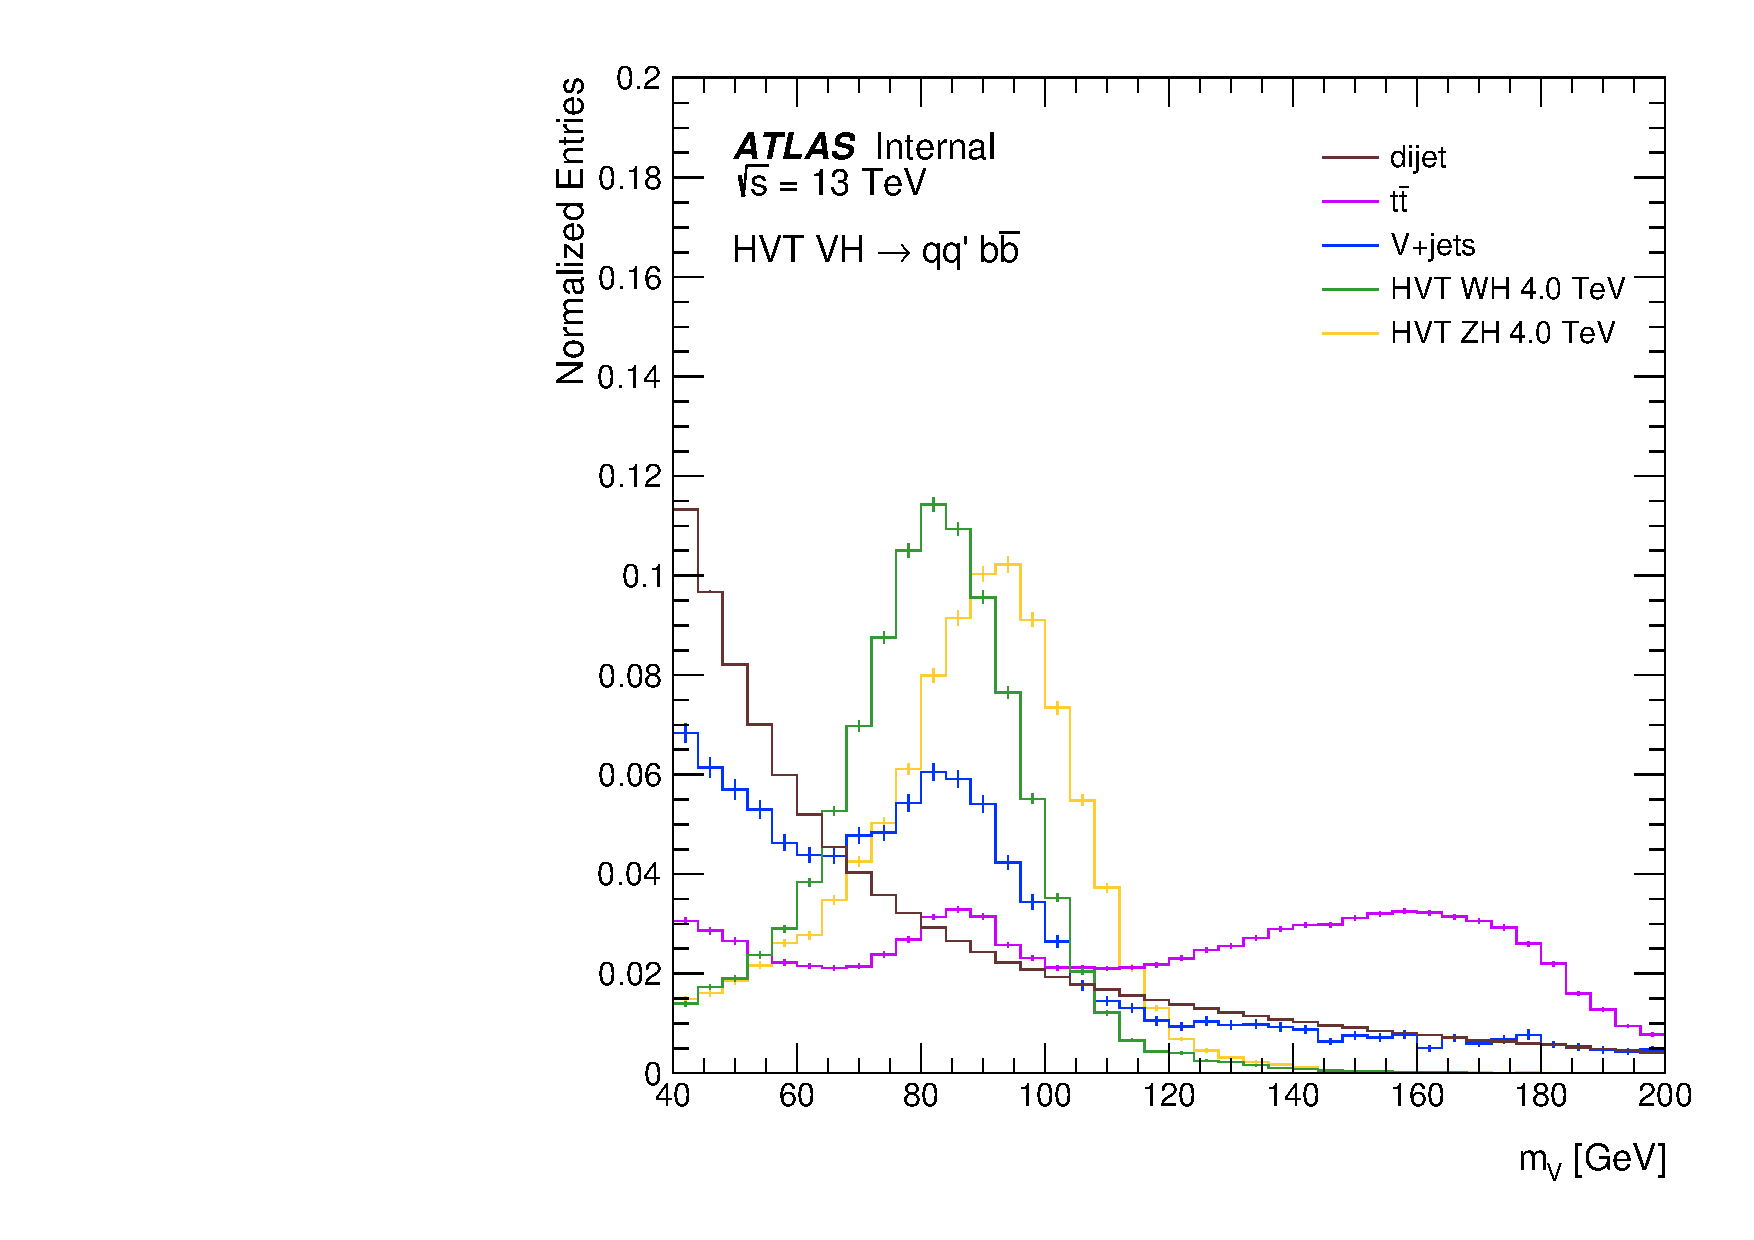
\includegraphics[width=0.49\textwidth]{VHqqbb_SimpleSigBkgMC_mV.pdf}
\end{center}
\caption{Vector boson candidate jet mass, as measured in signal and background MC samples, normalized to unity. Only pre-selection is applied, as described in Section~\ref{subsec:presel}.}
\label{fig:simple_mc_mV}
\end{figure}

\begin{figure}[htbp!]
\begin{center}
    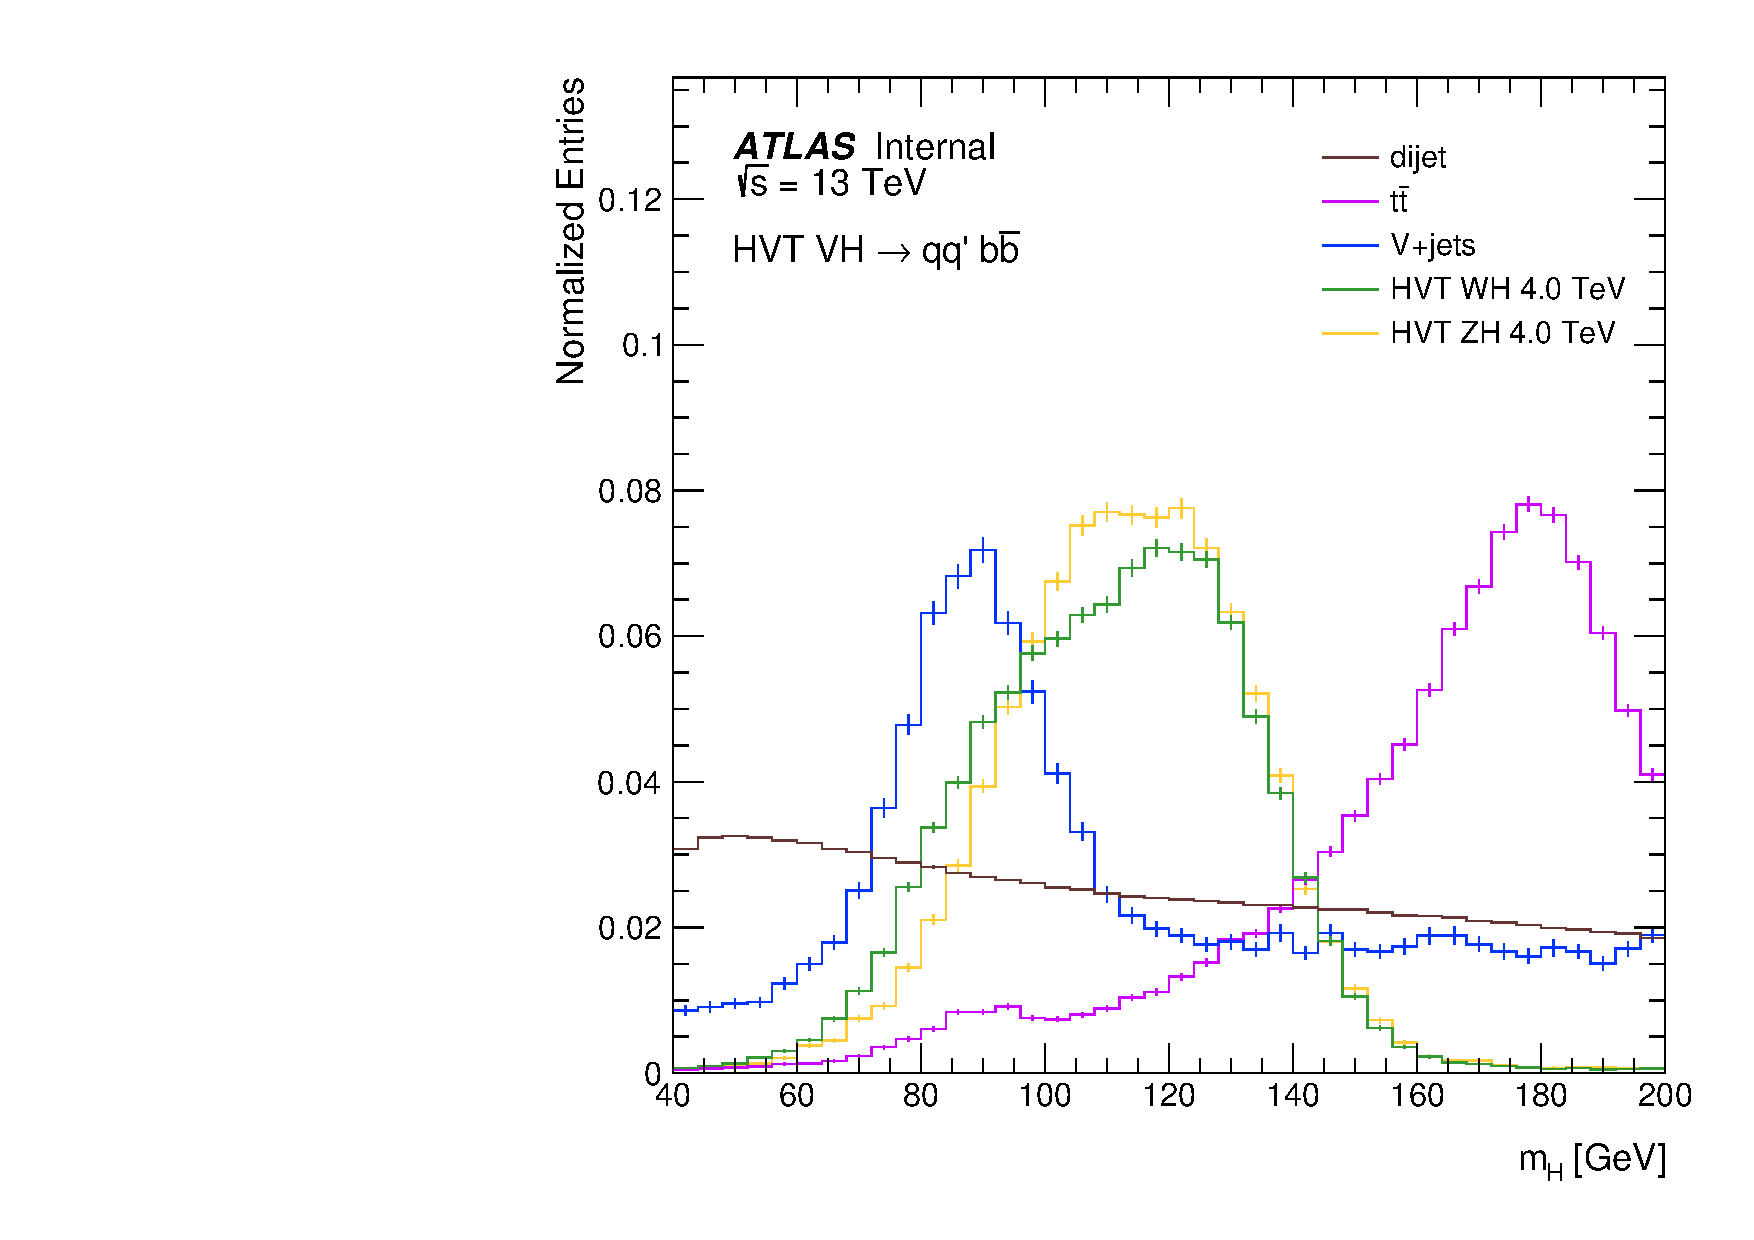
\includegraphics[width=0.49\textwidth]{VHqqbb_SimpleSigBkgMC_mH.pdf}
\end{center}
\caption{Higgs candidate jet mass, as measured in signal and background MC samples, normalized to unity. Only pre-selection is applied, as described in Section~\ref{subsec:presel}. }
\label{fig:simple_mc_mH}
\end{figure}

\begin{figure}[htbp!]
\begin{center}
    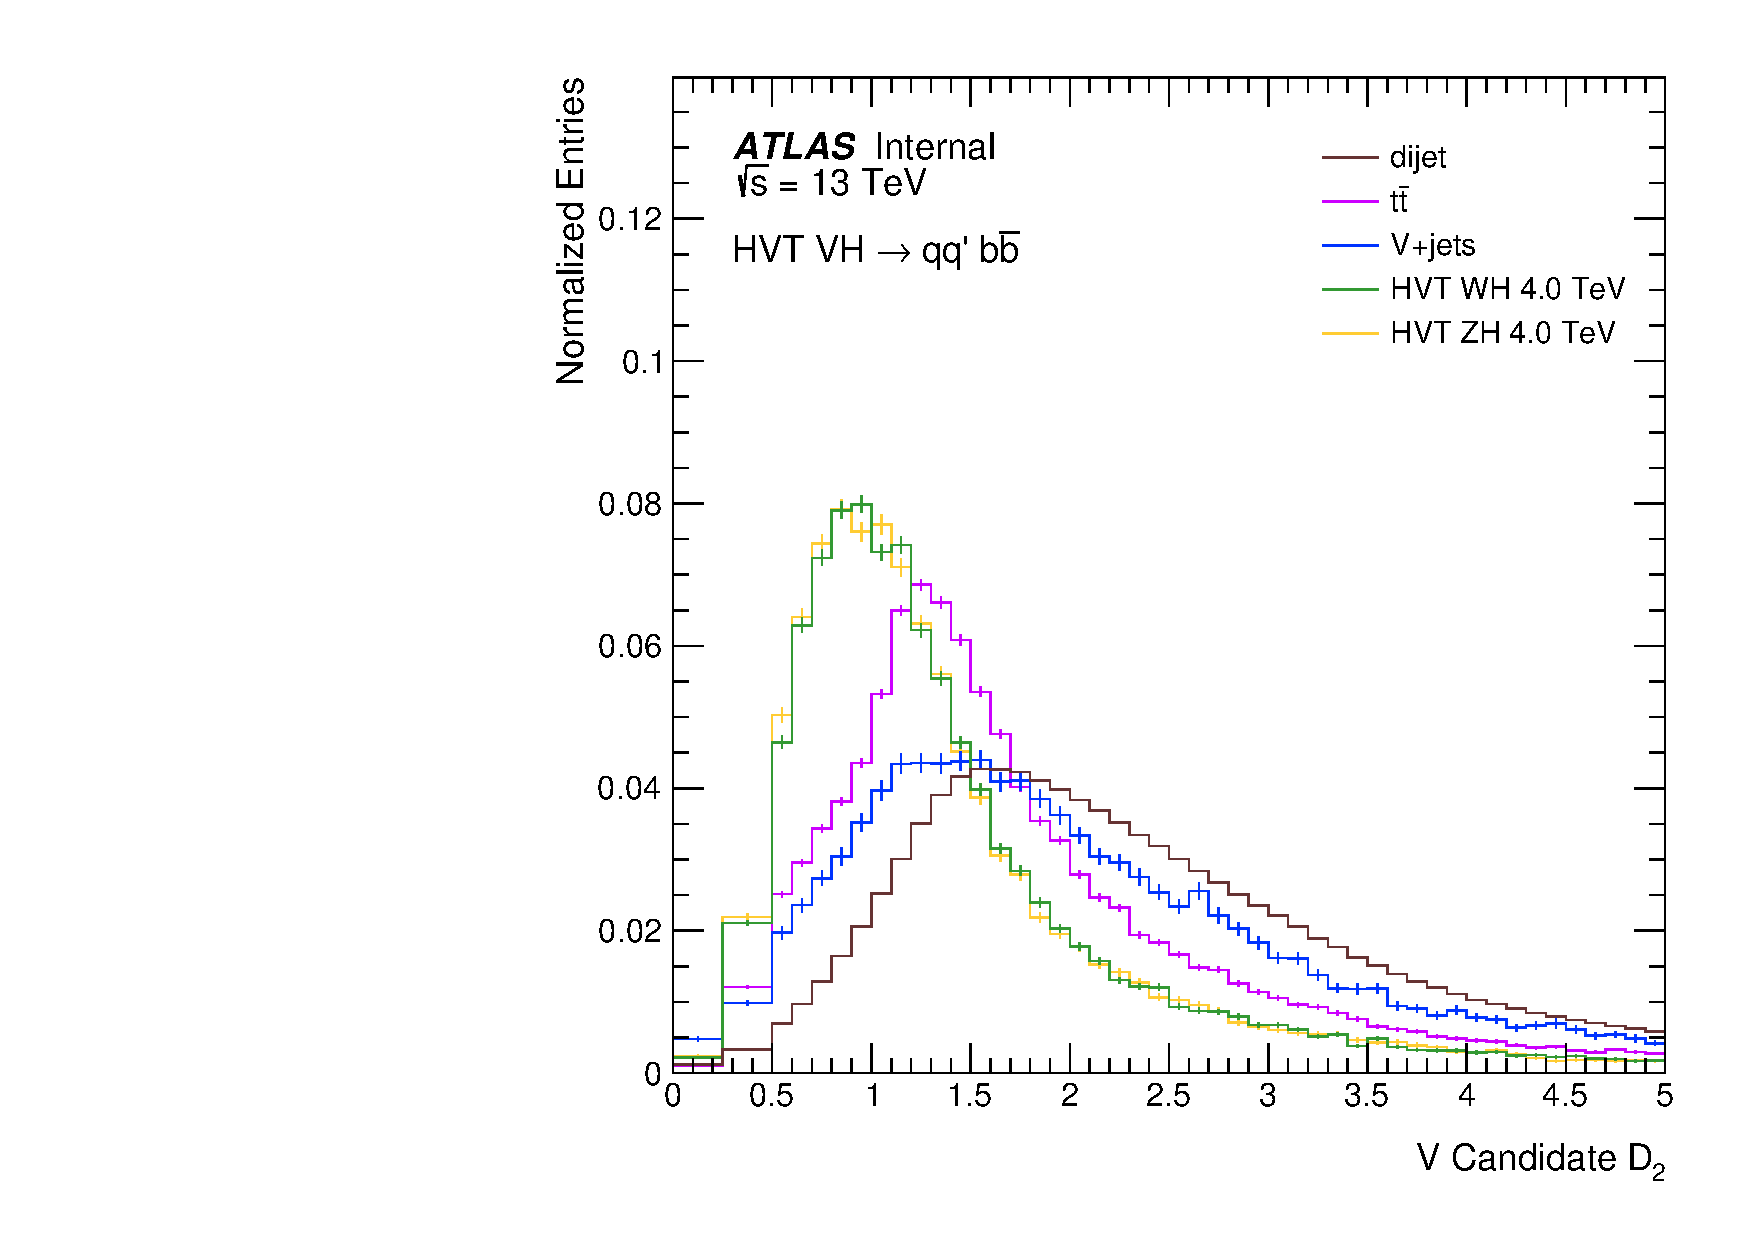
\includegraphics[width=0.49\textwidth]{VHqqbb_SimpleSigBkgMC_d2V.pdf}
\end{center}
\caption{Vector boson candidate jet \d2, as measured in signal and background MC samples, normalized to unity. Only pre-selection is applied, as described in Section~\ref{subsec:presel}. }
\label{fig:simple_mc_d2V}
\end{figure}

\begin{figure}[htbp!]
\begin{center}
    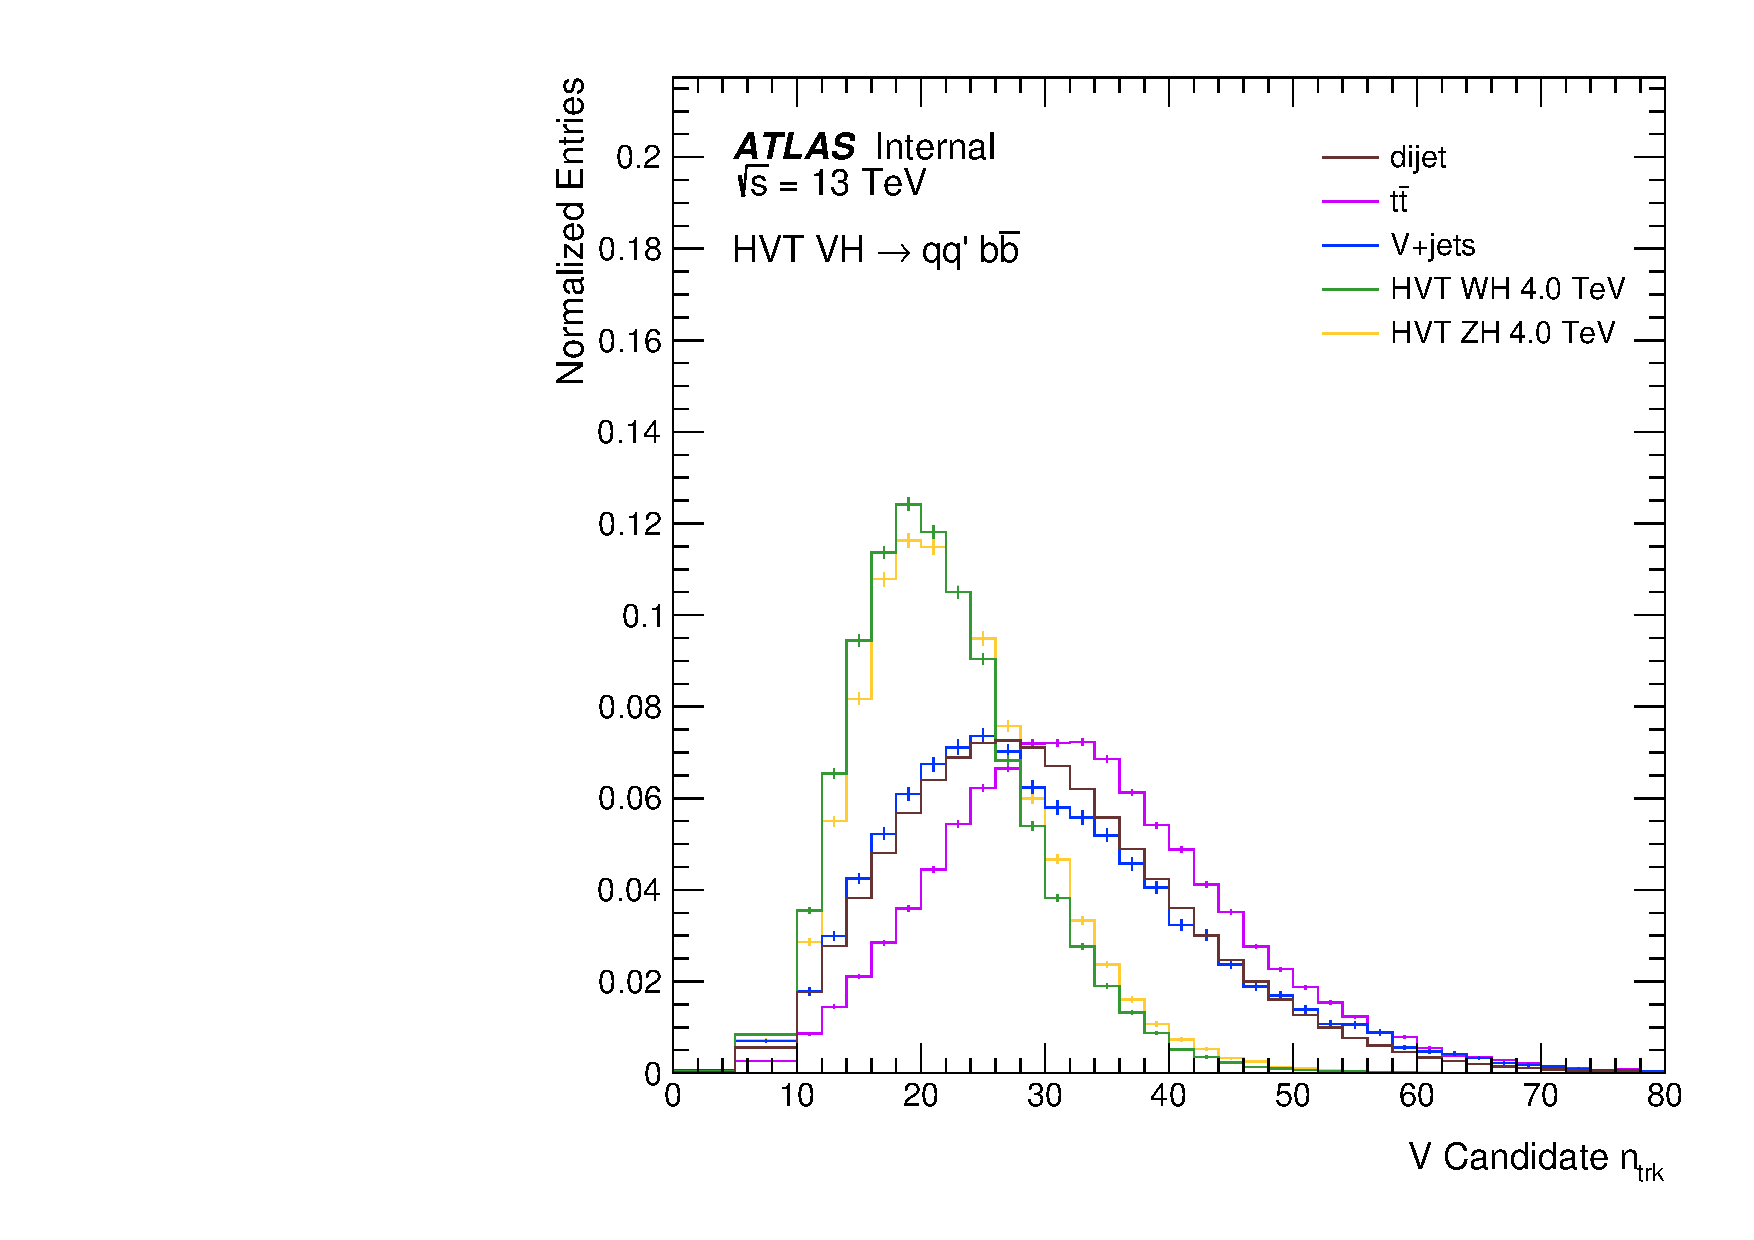
\includegraphics[width=0.49\textwidth]{VHqqbb_SimpleSigBkgMC_ntrkVVJJ_V.pdf}
\end{center}
\caption{Vector boson candidate jet \ntrk, as measured in signal and background MC samples, normalized to unity. Only pre-selection is applied, as described in Section~\ref{subsec:presel}. }
\label{fig:simple_mc_ntrkV}
\end{figure}

\begin{figure}[htbp!]
\begin{center}
    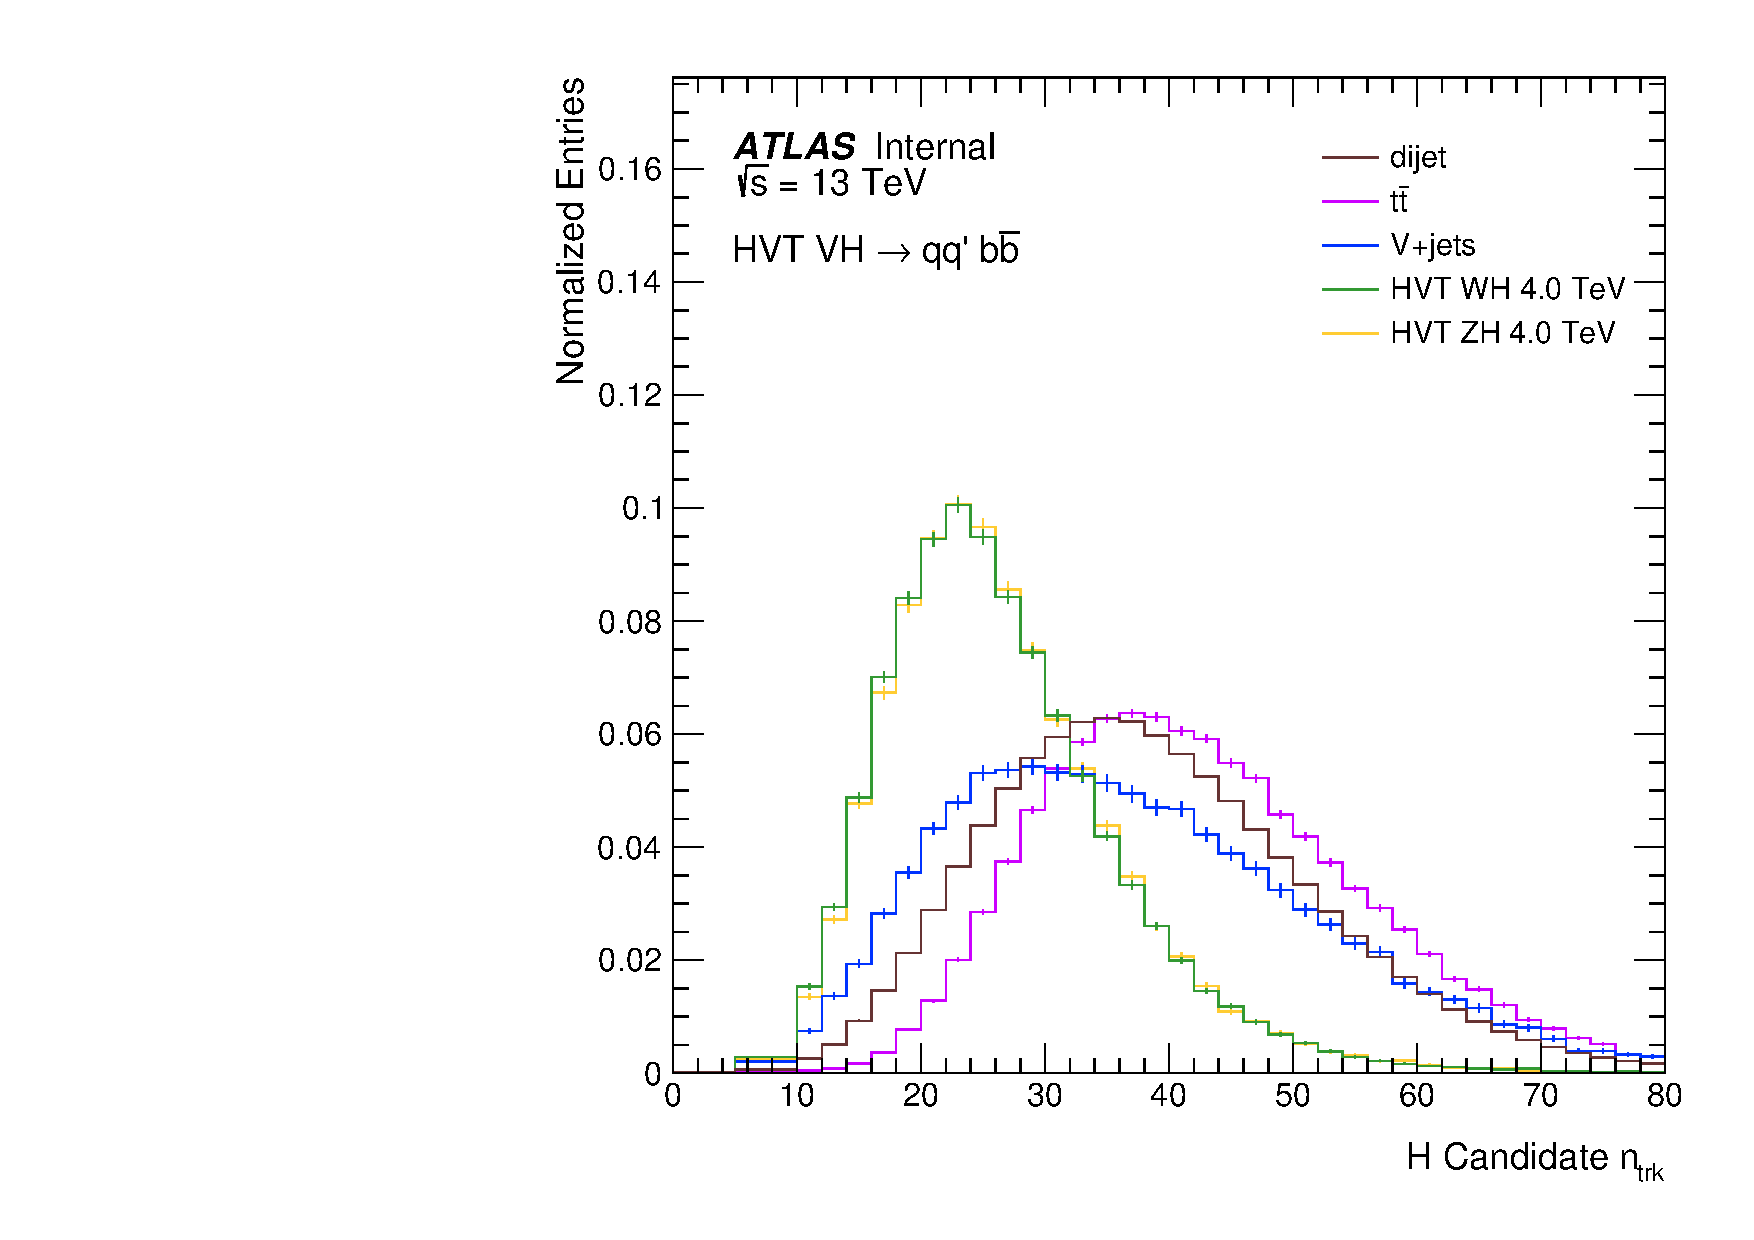
\includegraphics[width=0.49\textwidth]{VHqqbb_SimpleSigBkgMC_ntrkVVJJ_H.pdf}
\end{center}
\caption{Higgs candidate jet \ntrk, as measured in signal and background MC samples, normalized to unity. Only pre-selection is applied, as described in Section~\ref{subsec:presel}. }
\label{fig:simple_mc_ntrkH}
\end{figure}

\begin{figure}[htbp!]
\begin{center}
    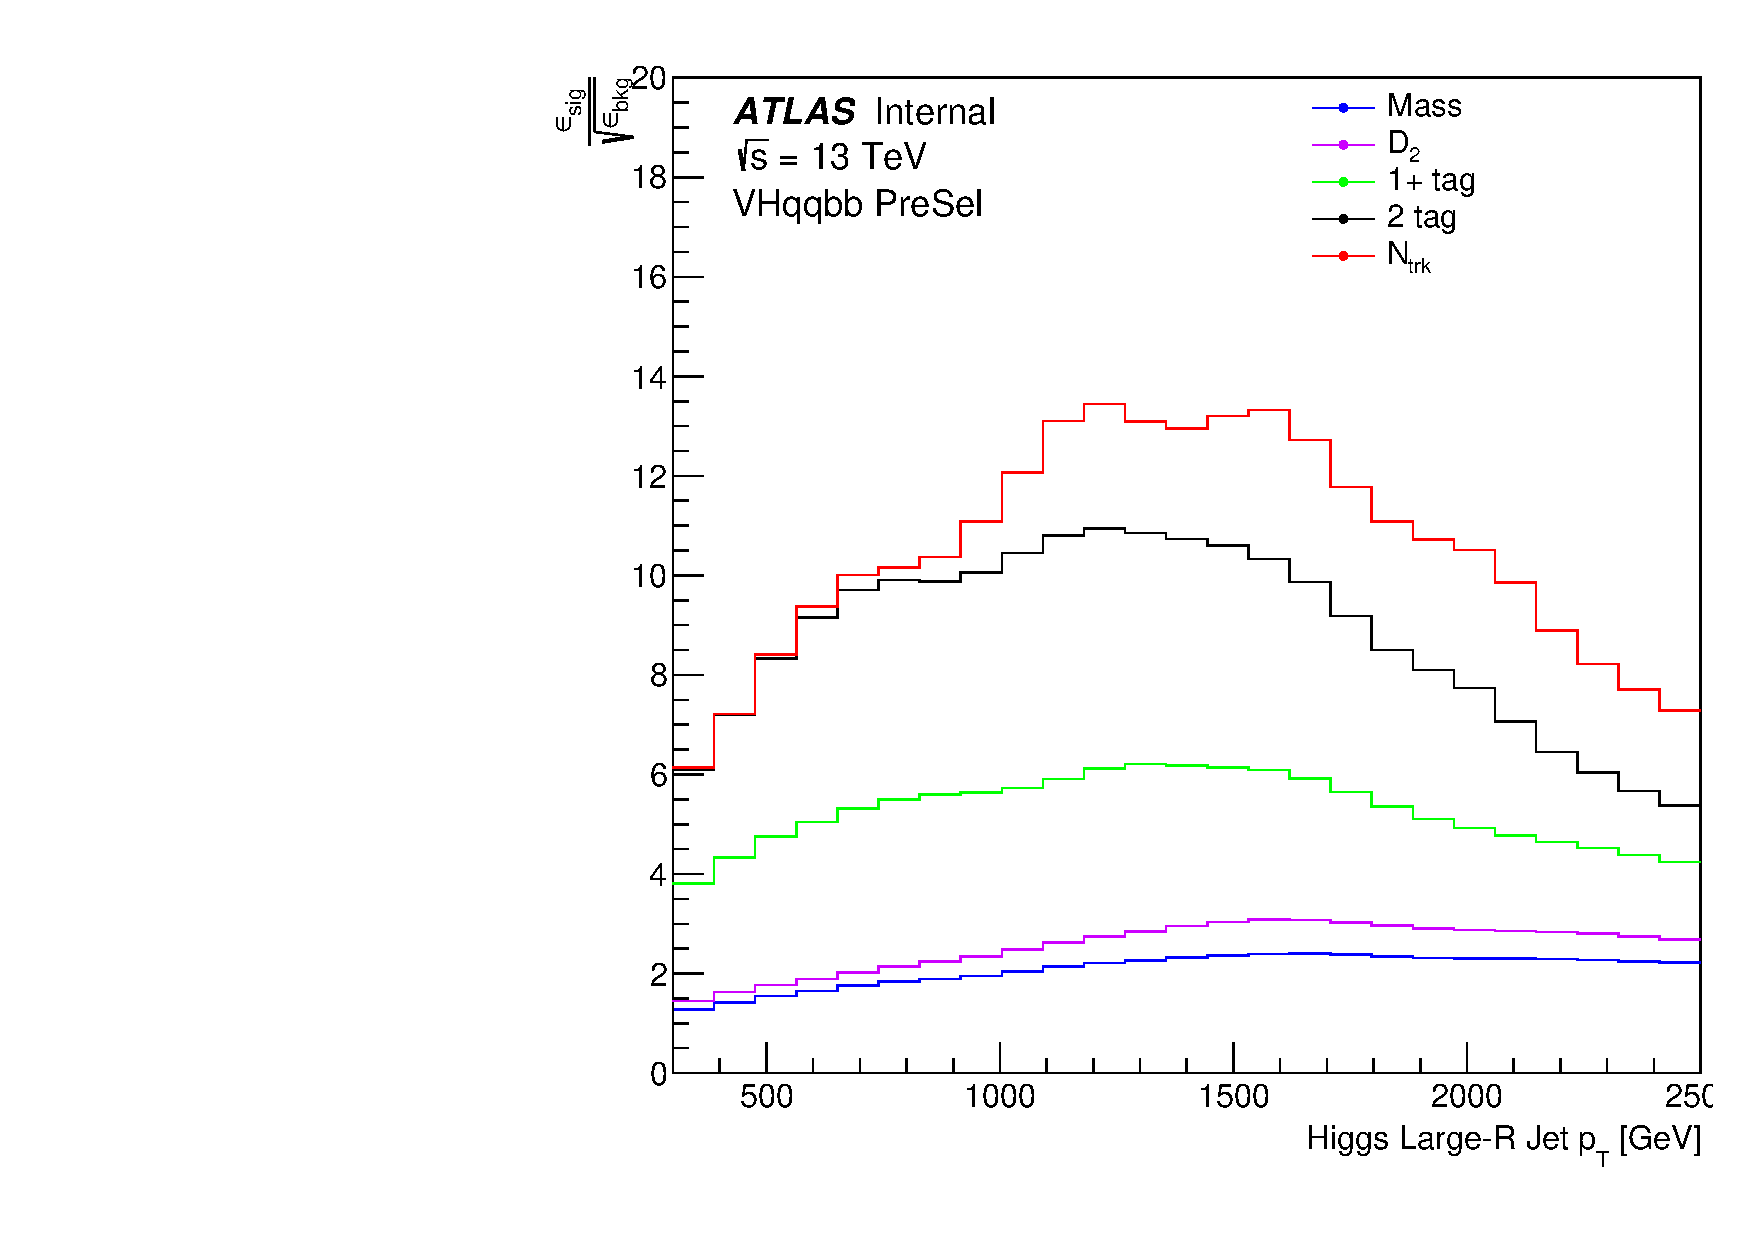
\includegraphics[width=0.49\textwidth]{PlotHTagSensitivityWithD2.pdf}
\end{center}
\caption{Sensitivity of optimized cuts for Higgs tagging. The optimized \d2 cut (violet) is included only for reference and not used in the final analysis due to lack of discrimination power.
    The cuts are cumulative, in the order listed in the legend, and the pre-selection described in Section~\ref{subsec:presel} is also applied.
}
\label{fig:htag_sens_d2}
\end{figure}

\subsubsection{Optimization Method}
\label{subsec:tagger_opt}
% The optimization method and motivation applied here was strongly influenced by the work done in the all-hadronic VV resonance search, and is documented in detail in the corresponding support note~\cite{VVJJSupport2019}.
% For this note we only discuss the method briefly and include extra information specifically relevant to this search.
%TODO: define 'subjet'
%TODO: cite or write out truth-matching criteria
Three separate taggers are derived for W, Z, and Higgs bosons utilizing a maximum significance expression \cite{punzi2003sensitivity} which is independent of signal cross-section: $\frac{\epsilon}{\frac{a}{2}+\sqrt{B}}$, where $\epsilon$ is the signal efficiency, $a$ is the sigma count number corresponding to a one-sided Gaussian significance, and $B$ is the background yield.
Smaller values of $a$ are more appropriate for limit-setting, while larger values optimize for maximum discovery potential.
A middle ground is chosen here and a value of $a = 3$ is used.
The optimization of all relevant variables is performed simultaneously for $W$, $Z$ and $H$ bosons.
In the case of the Higgs boson, separate optimization is performed for the case where 1 or 2 VR track jets pass the $b$-tagging criteria.
The inputs to the optimization include only a loose pre-selection, without any ~\dy12 or ~\mvh\ requirements.
Only signal events with proper V/H truth matching are included in the optimization, thus $\epsilon$ represents the fraction of truth-matched W/Z/H large-$R$ ~jets passing the selection.
The words 'events' and 'jets' here are interchangeable, due to the fact that there is a maximum of one W or Z or H boson per signal event.
An example plot of this sensitivity expression for the $[750,950]$ GeV \pt\ bin of the Higgs tagger optimization is shown in Figure~\ref{fig:higgs_opt_sens}.

% Explain 'VVJJ'
For W/Z bosons a three-dimensional tagger is derived utilizing jet mass, \d2, and \ntrk.
The \d2 and \ntrk cuts are both upper bound cuts, while the jet mass cuts form a two-sided window.
In the case of Higgs tagging a two-dimensional set of jet mass and \ntrk cuts is derived.
The \d2 observable was not included in the Higgs optimization due to lack of discriminating power in conjunction with $b$-tagging.

Due to the correlation of each optimization variable with large-R jet \pt, each separate tagger is derived as a set of maximum sensitivity cuts in bins of large-R jet \pt.
After optimization of these cuts, they are smoothed by fitting with the following expression: $\sqrt{\frac{A^2}{(\pt-B)^2} + C^2(\pt-D)^2}$.
Both terms are first order approximations for different factors impacting the measurement resolution of the jet mass.
The first term accounts for energy resolution, which worsens at low \pt, and the second for angular resolution, which worsens at high \pt.
While this expression is physically motivated for the mass cut, it works equally well for the \ntrk cut.

The optimized Higgs mass and \ntrk cuts are shown in Figure ~\ref{fig:higgs_tagger_cuts}, and the successive efficiency of each cut is shown in Figure ~\ref{fig:higgs_tagger_eff}.
The optimized W/Z mass and \d2 cuts from VVJJ are shown in Figure ~\ref{fig:vvjj_wz_tagger_mass_d2_cuts}.
The optimized W/Z \ntrk cuts are shown in Figure ~\ref{fig:wz_tagger_ntrk_cuts}.

\begin{figure}[htbp!]
\begin{center}
    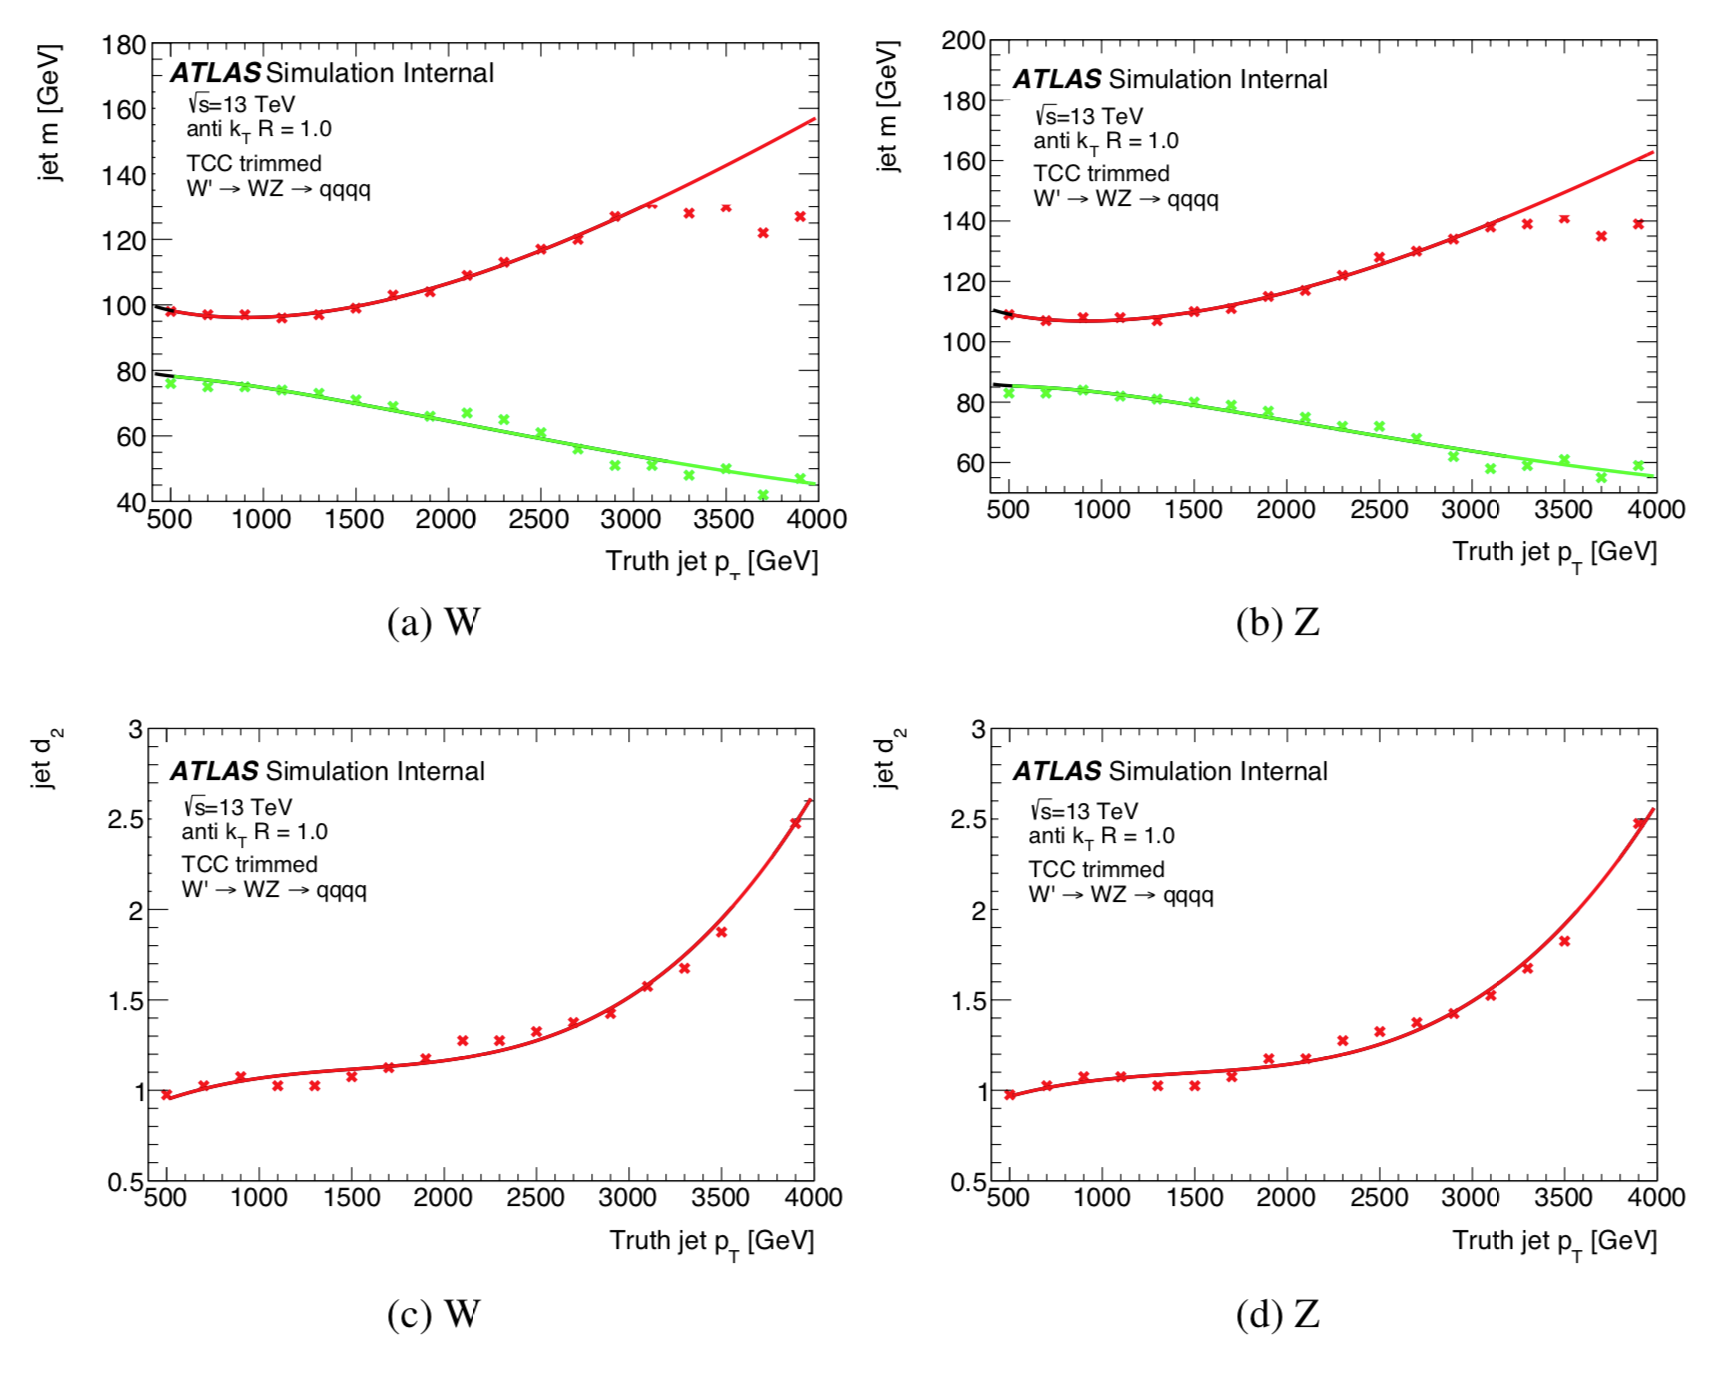
\includegraphics[width=0.9\textwidth]{VVJJ_Mass_d2_WZ_cuts.png}
\end{center}
\caption{W/Z boson tagging cuts derived by the VVJJ group for mass (a) (b) and \d2 (c) (d).}
\label{fig:vvjj_wz_tagger_mass_d2_cuts}
\end{figure}

\begin{figure}[htbp!]
\begin{center}
    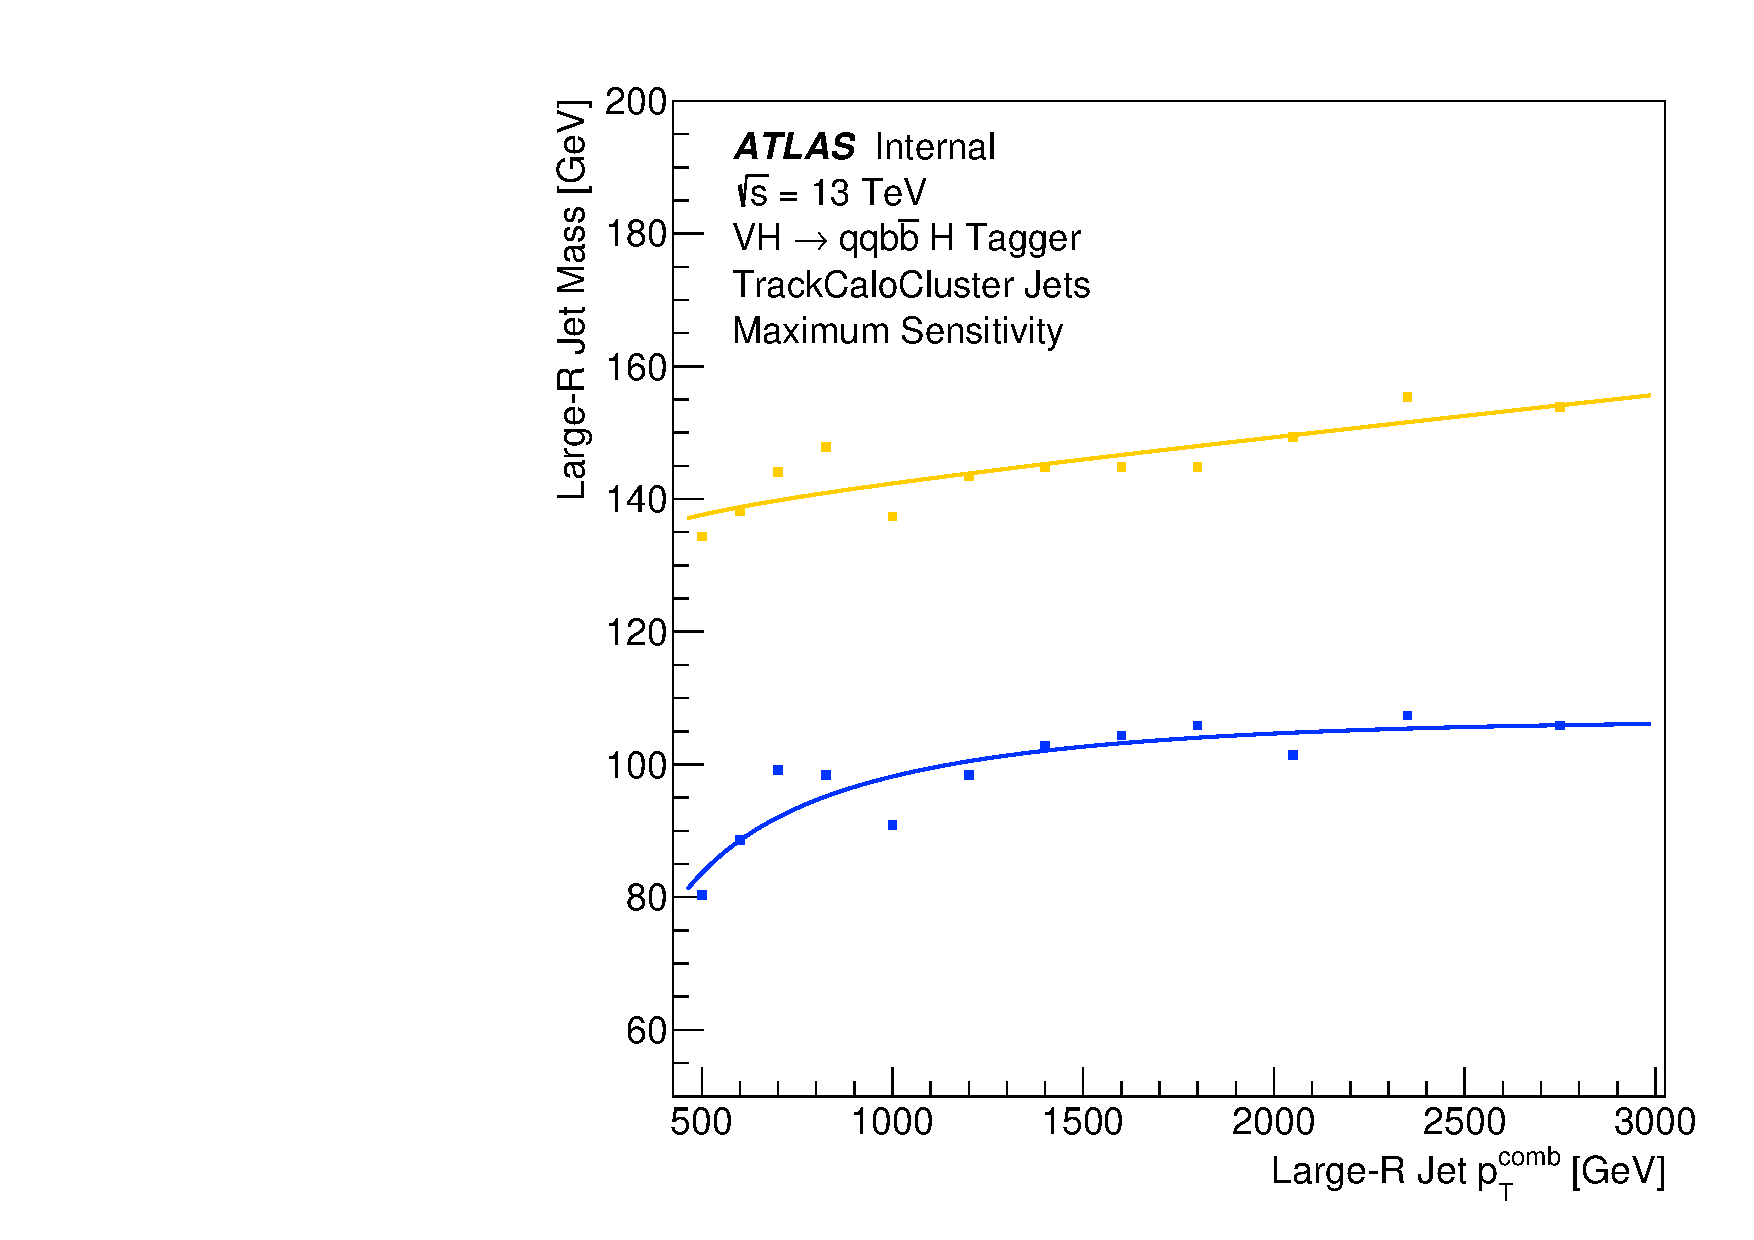
\includegraphics[width=0.49\textwidth]{VHqqbbOptimizedBosonTagger_H_mass_1tag.pdf}
    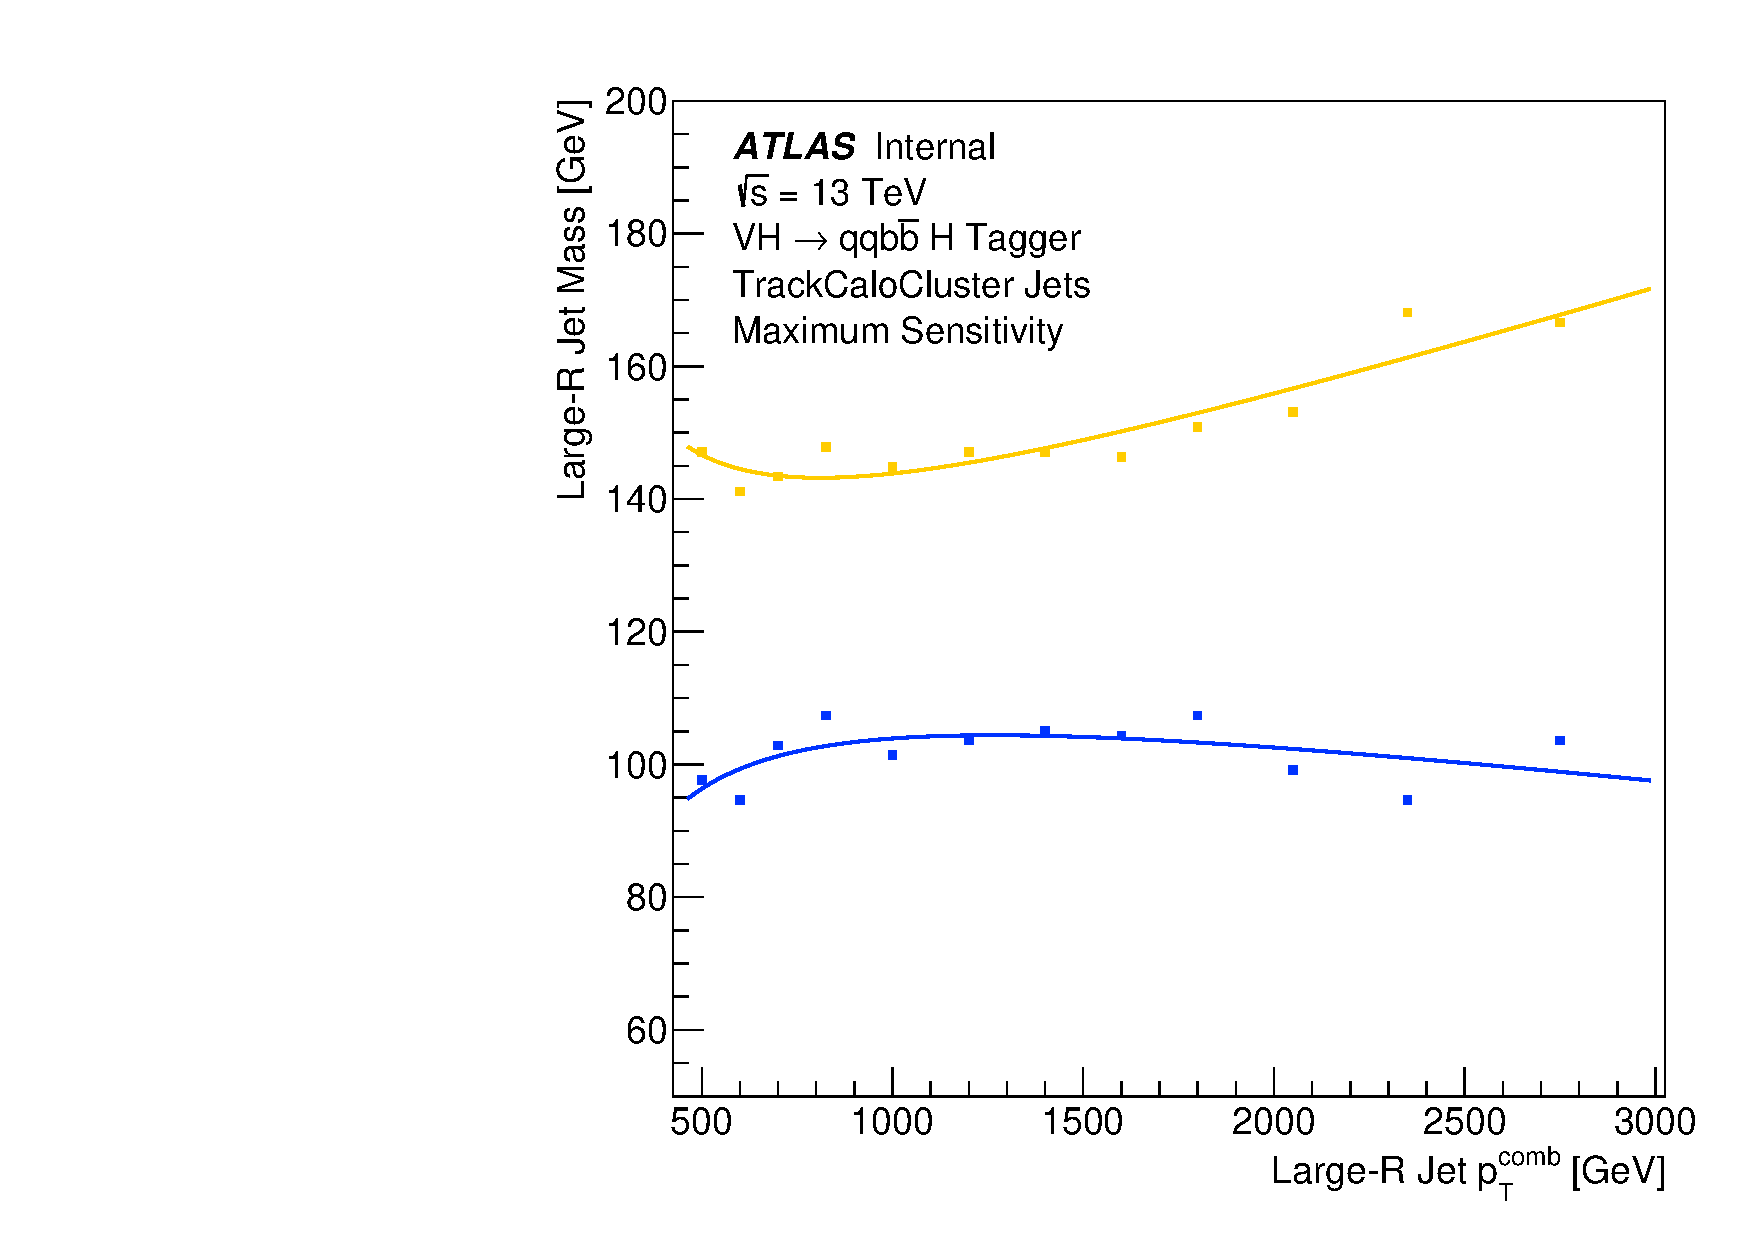
\includegraphics[width=0.49\textwidth]{VHqqbbOptimizedBosonTagger_H_mass_2tag.pdf} \\
    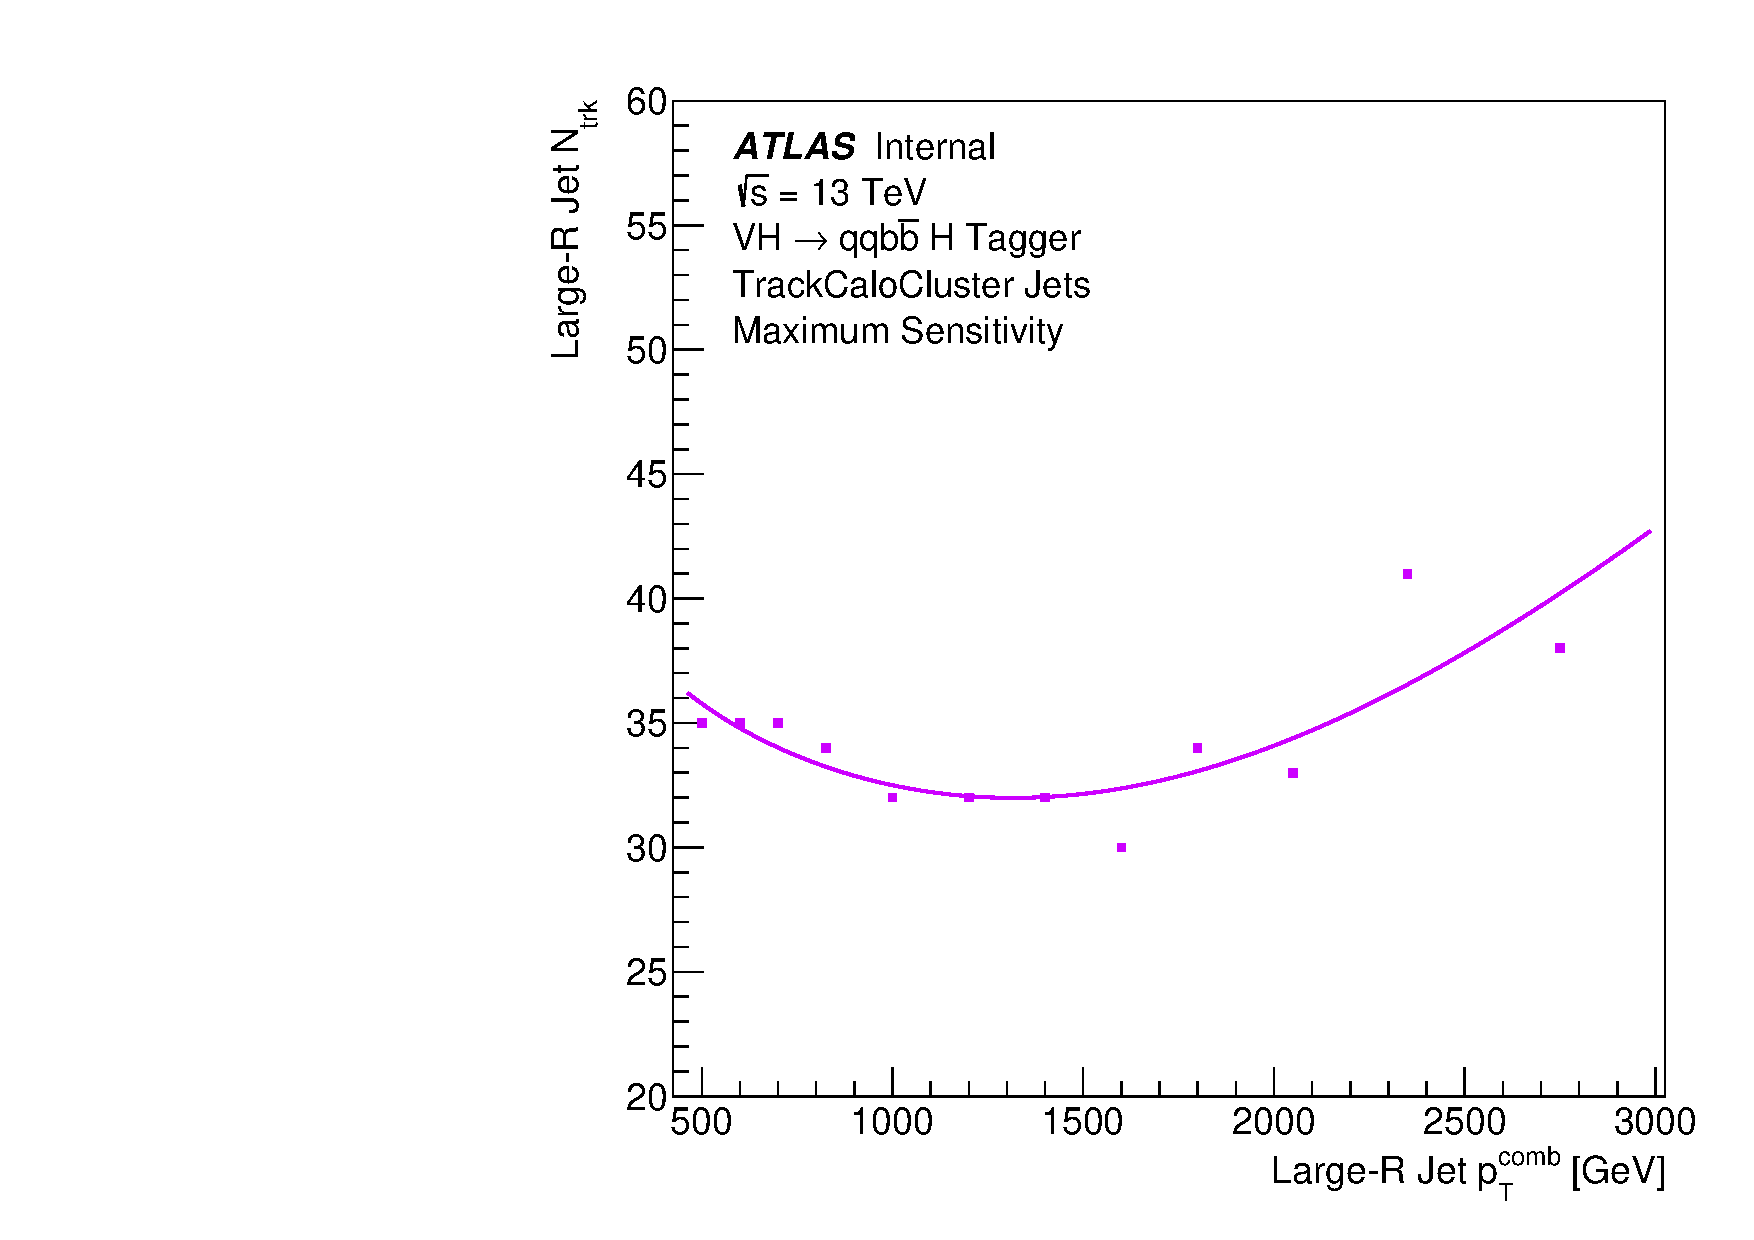
\includegraphics[width=0.49\textwidth]{VHqqbbOptimizedBosonTagger_H_ntrk_1tag.pdf}
    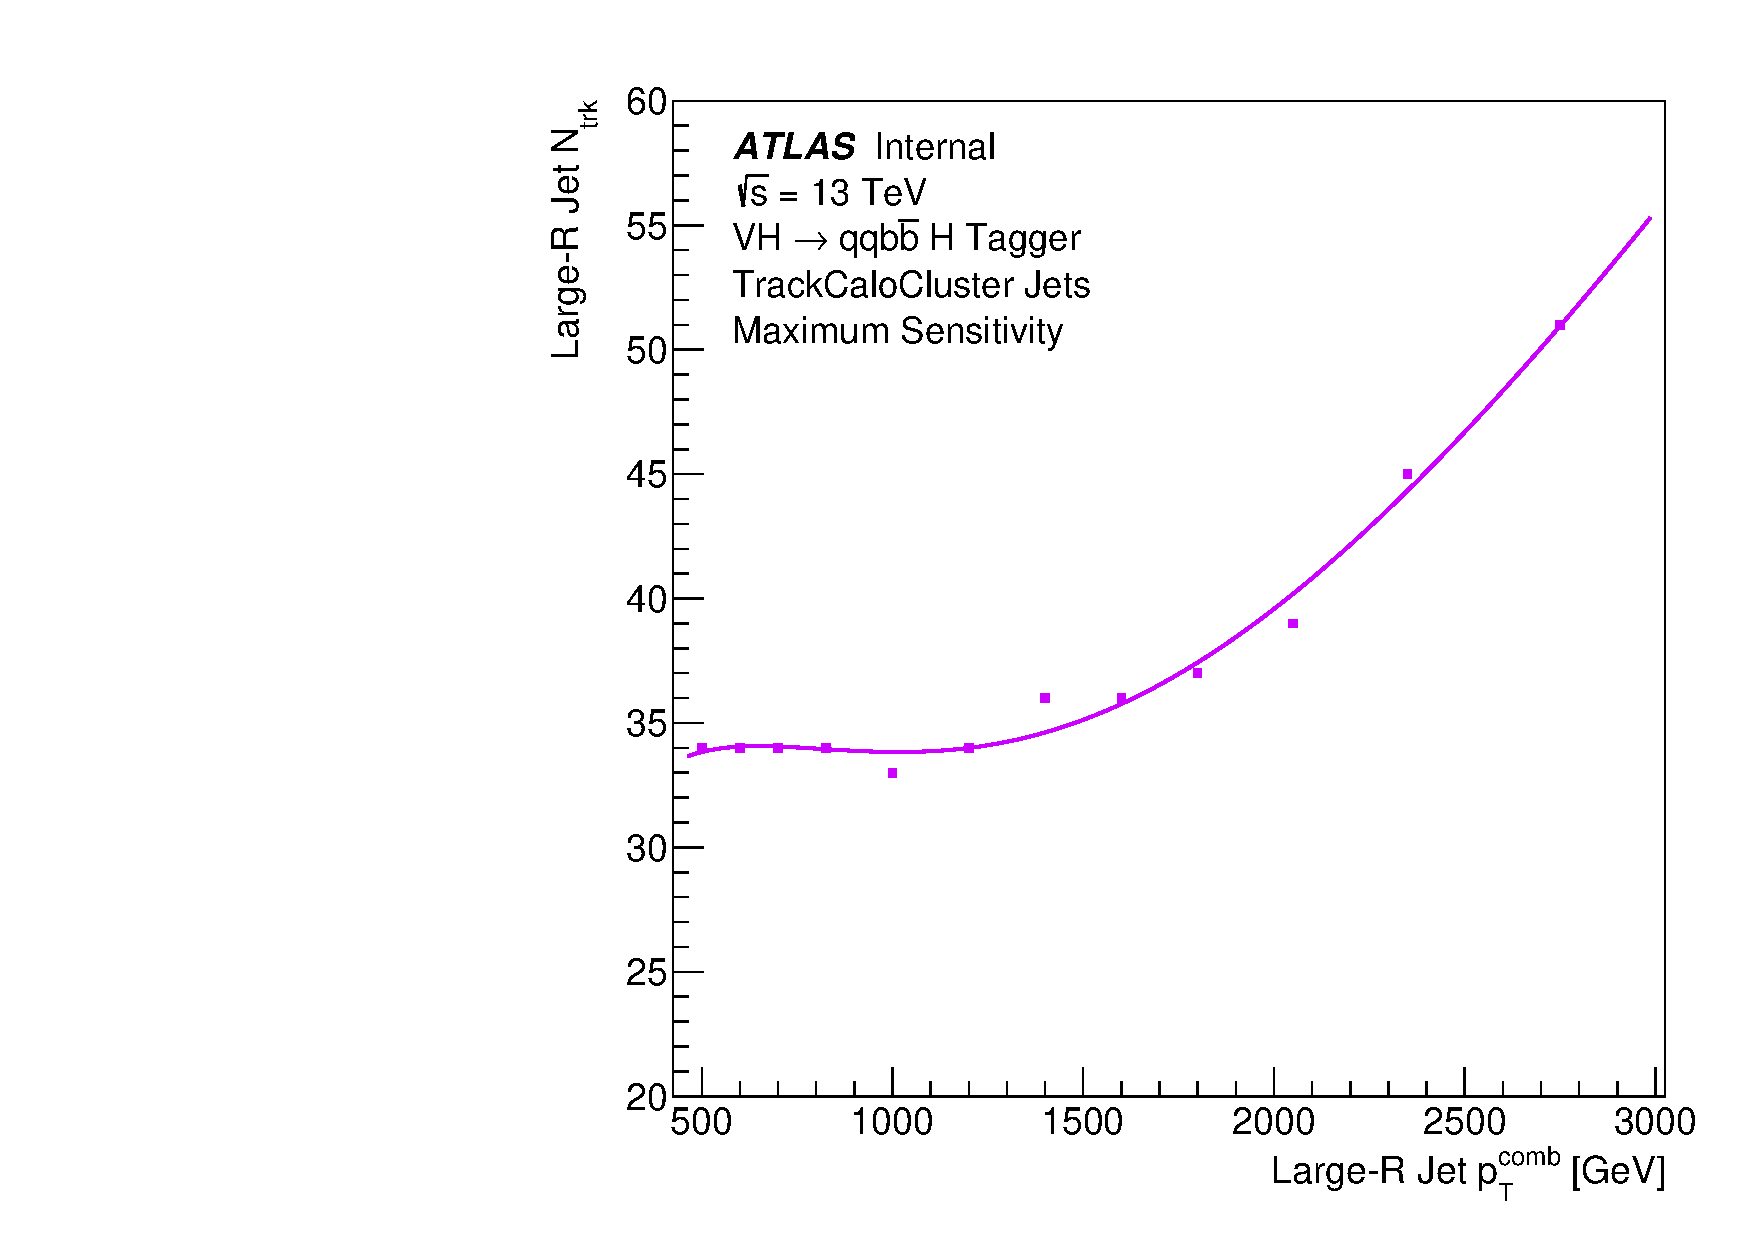
\includegraphics[width=0.49\textwidth]{VHqqbbOptimizedBosonTagger_H_ntrk_2tag.pdf}
\end{center}
\caption{Higgs tagging cuts derived via the method described in Section~\ref{subsec:tagger_opt}. Both the 1-tag (left) and 2-tag (right) channels are shown for the mass (top row) and \ntrk (bottom row) cuts.}
\label{fig:higgs_tagger_cuts}
\end{figure}

\begin{figure}[htbp!]
\begin{center}
    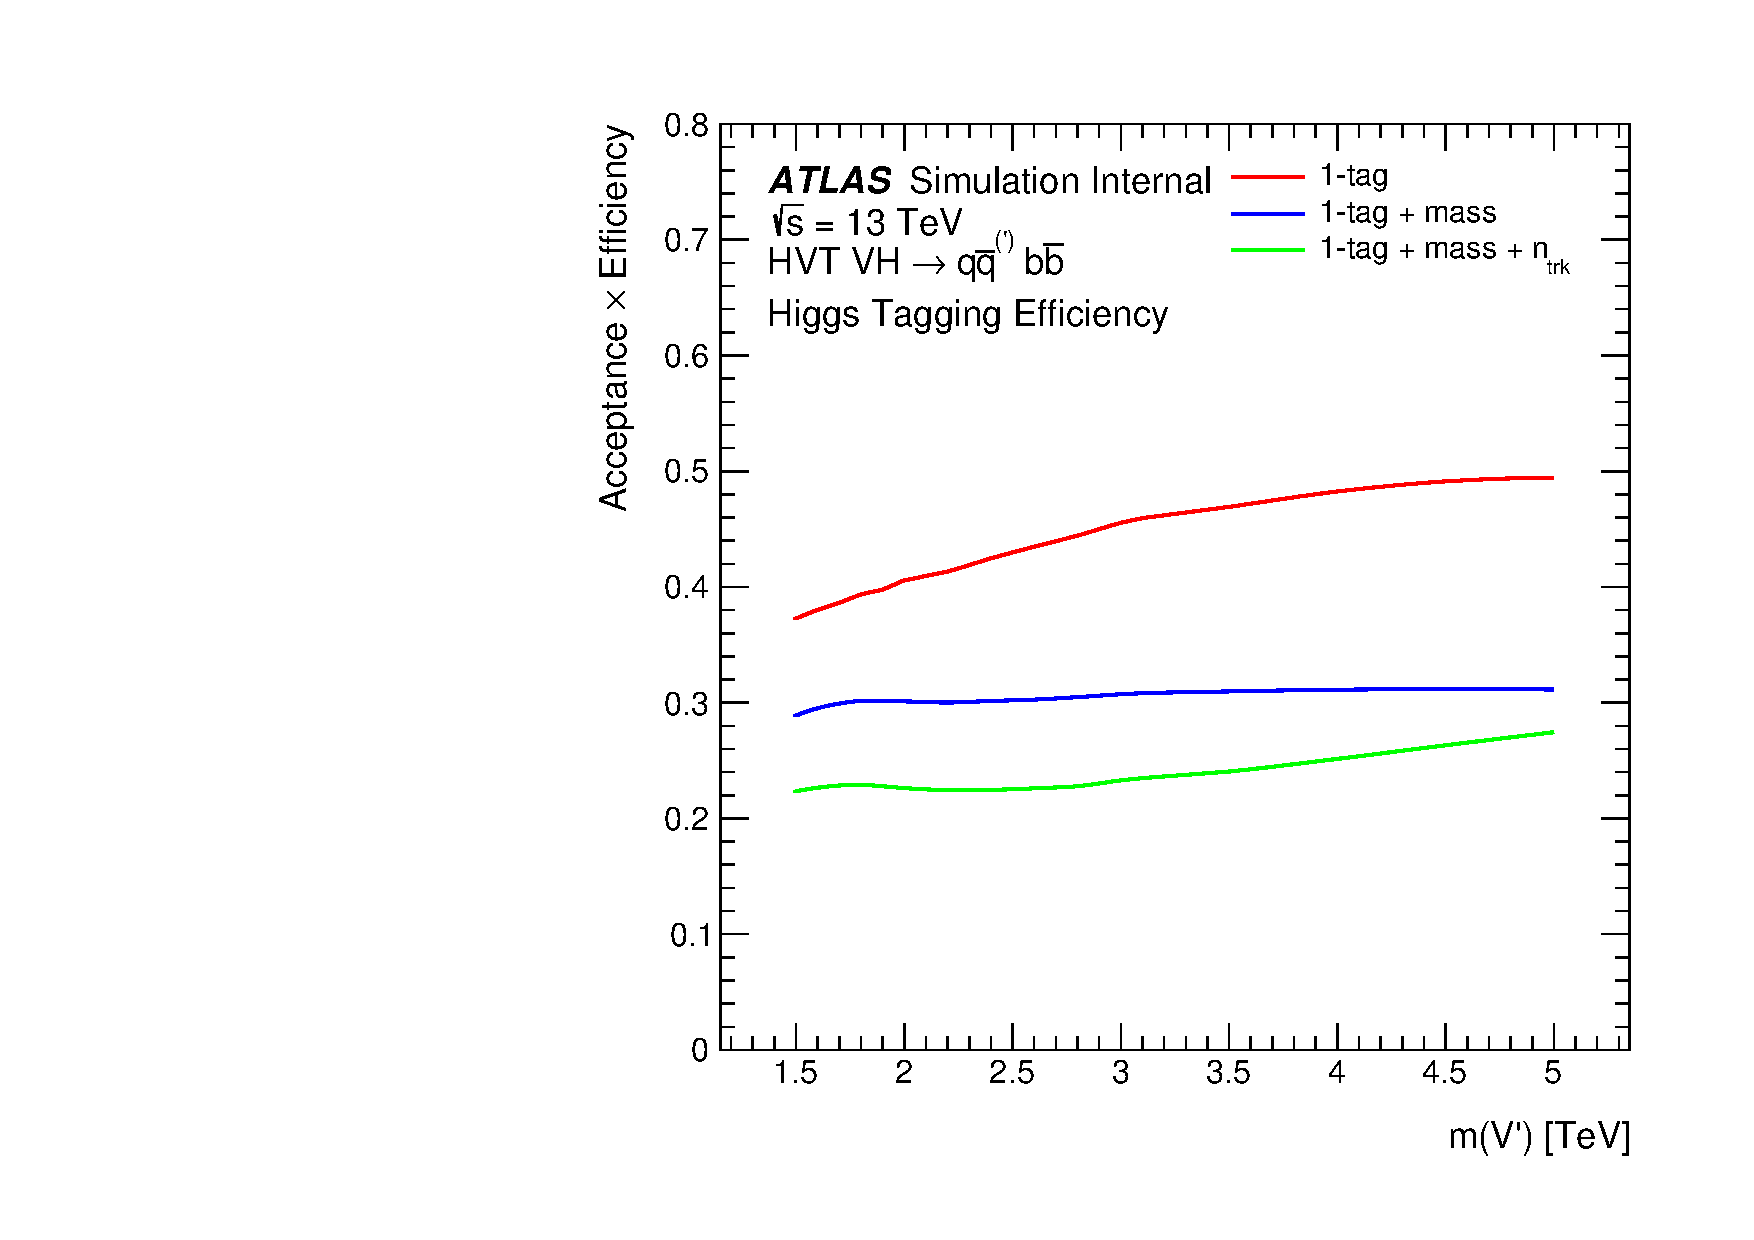
\includegraphics[width=0.49\textwidth]{VHqqbb_HiggsTaggingEff_1tag.pdf}
    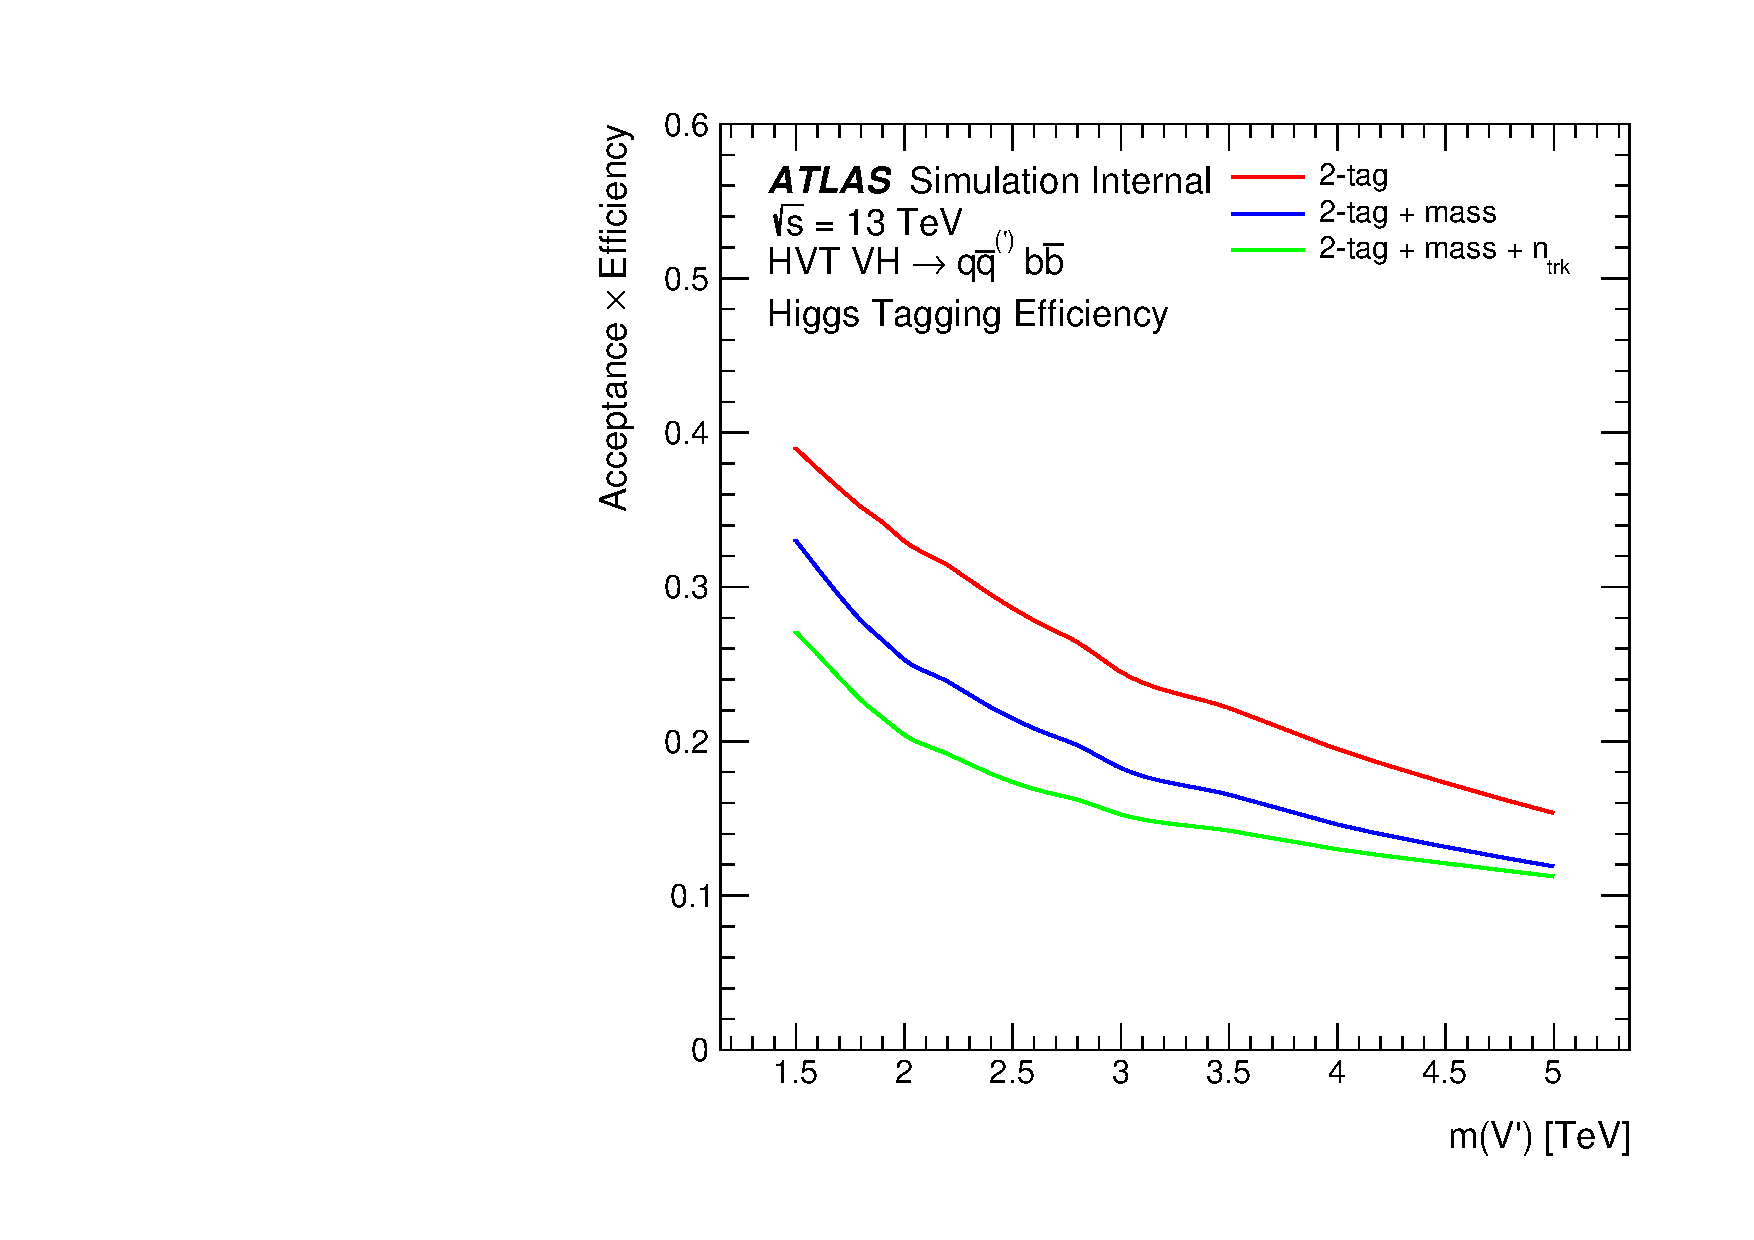
\includegraphics[width=0.49\textwidth]{VHqqbb_HiggsTaggingEff_2tag.pdf}
\end{center}
\caption{Efficiency times acceptance (relative to pre-selection) for each successive Higgs tagging cut derived via the method described in Section~\ref{subsec:tagger_opt}. Both the 1-tag (left) and 2-tag (right) channels are shown and $b$-tagging scale factors are applied.}
\label{fig:higgs_tagger_eff}
\end{figure}

\begin{figure}[htbp!]
\begin{center}
    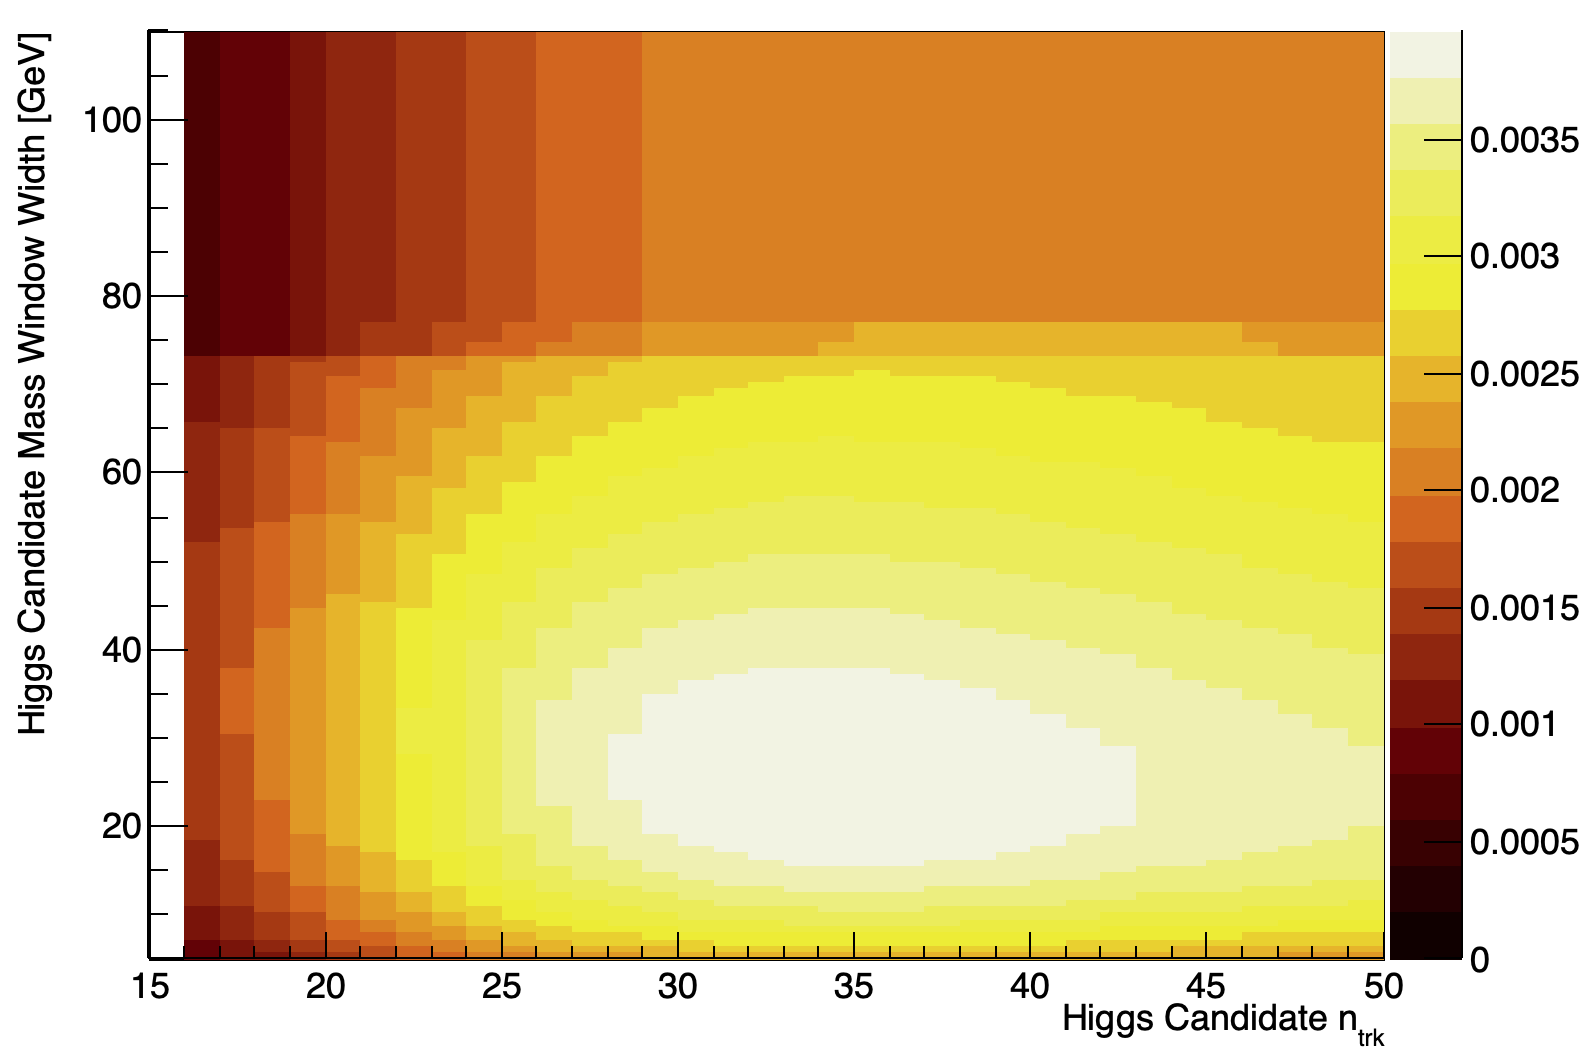
\includegraphics[width=0.6\textwidth]{VHqqbb_HiggsOpSens_pT750to900GeV.png}
\end{center}
\caption{Example sensitivity map for the [750, 950] GeV \pt\ bin of the Higgs tagger optimization. The location of the maximum of this 2-dimensional distribution determines the mass and \ntrk cuts for this \pt\ bin.}
\label{fig:higgs_opt_sens}
\end{figure}

\begin{figure}[htbp!]
\begin{center}
    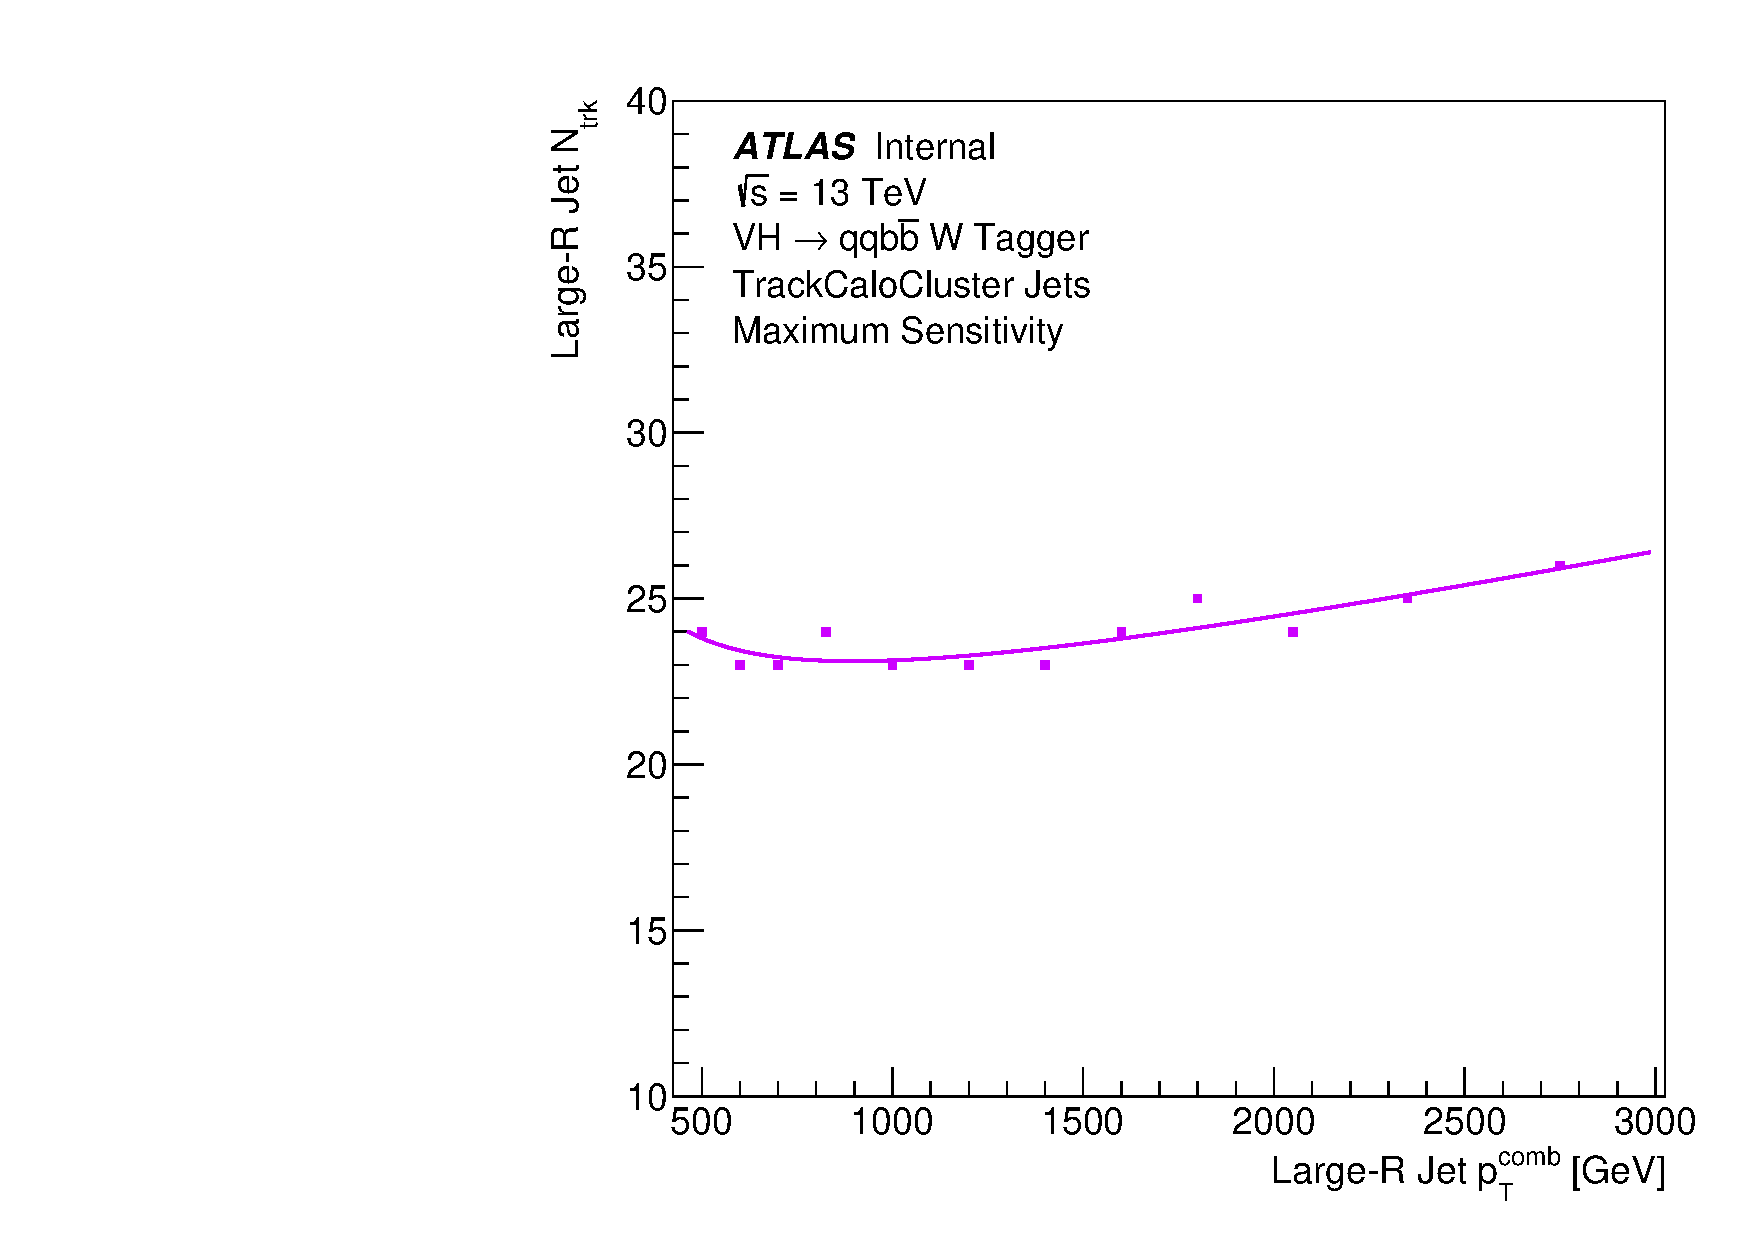
\includegraphics[width=0.49\textwidth]{VHqqbbOptimizedBosonTagger_W_ntrk.pdf}
    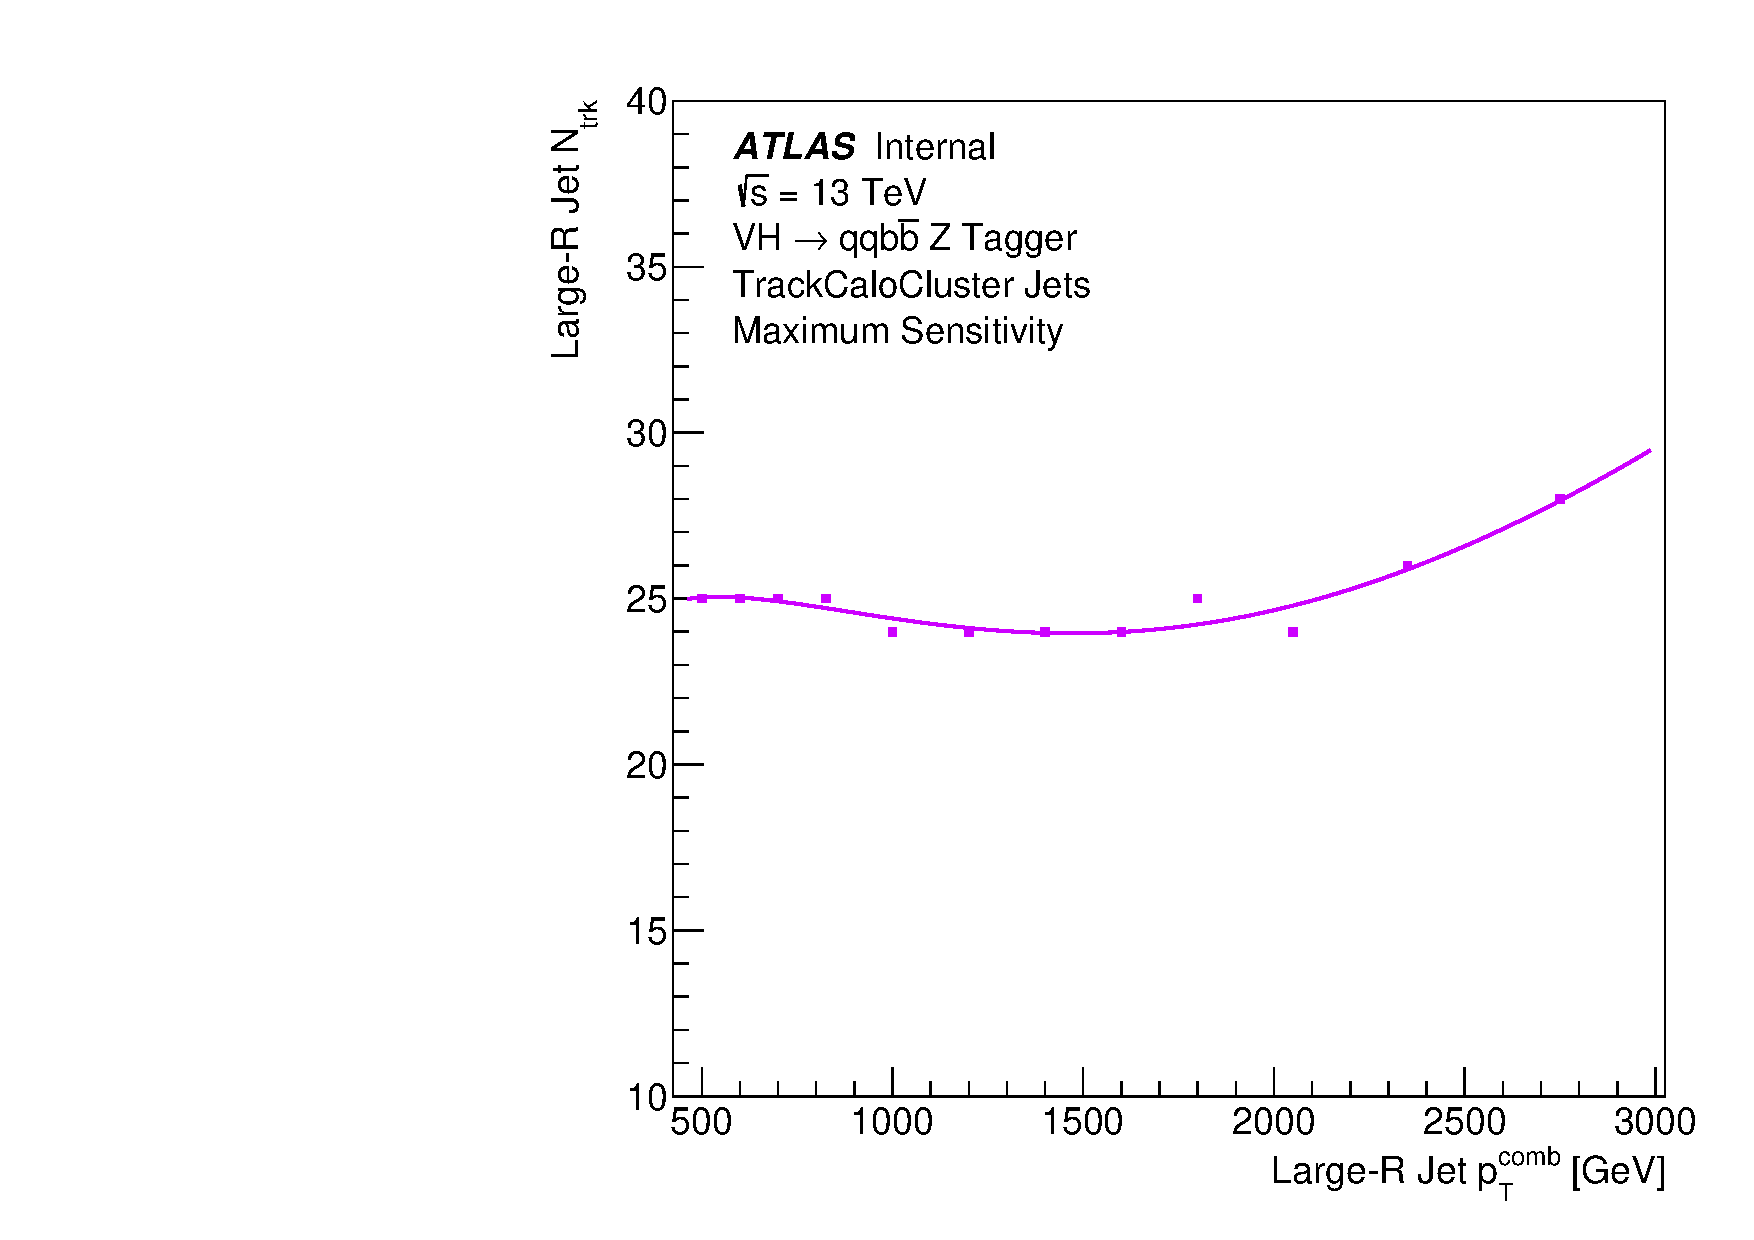
\includegraphics[width=0.49\textwidth]{VHqqbbOptimizedBosonTagger_Z_ntrk.pdf}
\end{center}
\caption{Vector boson \ntrk cuts derived via the method described in Section~\ref{subsec:tagger_opt}. Both W boson (left) and Z boson (right) cuts are shown.}
\label{fig:wz_tagger_ntrk_cuts}
\end{figure}

\subsection{Signal Regions}
\label{sec:SR}
Events passing the event selection cuts and containing a Higgs-boson and a vector-boson candidate, as listed in Table \ref{tab:selection}, are further categorized according to the number of $b$-tagged VR track-jets that are associated to the $H$-tagged jet.
For each of the $WH$ and $ZH$ final states (non-orthogonal, as identified by the different mass window cuts described in Sec.\ref{subsec:tagger_opt}), two independent signal region channels are defined: 1-tag and 2-tag.

The \mvh\ distributions for different signal mass points are shown in Figure \ref{fig:signalMjj}, for events selected in the 1-tag and 2-tag signal regions.
Figure~\ref{fig:effBkg} shows the efficiency as measured in the MC simulation for each of the background processes.
The efficiency of each selection cut for $WH$ and $ZH$ signal processes is shown on Figure \ref{fig:effVH}.
In addition, the efficiency curves in the final 1-tag and 2-tag $WH$ and $ZH$ signal regions are shown in Figure~\ref{fig:effcurve}.
As one can see, the orthogonal 1-tag and 2-tag signal regions are complementary to each other for the search.
A more detailed breakdown of the cutflow for the WH 2.0 TeV and ZH 4.0 TeV signal samples can be found in Tables \ref{tab:wh_2TeV_cutflow} and \ref{tab:zh_4TeV_cutflow}.

While the individual 1-tag/2-tag channels are orthogonal, the WH/ZH signal regions themselves are not.
As measured in data there is 38.3\% SRWH/SRZH overlap in the 1-tag channel, and 39.6\% SRWH/SRZH overlap in the 2-tag channel.

\begin{figure}[htbp!]
\begin{center}
    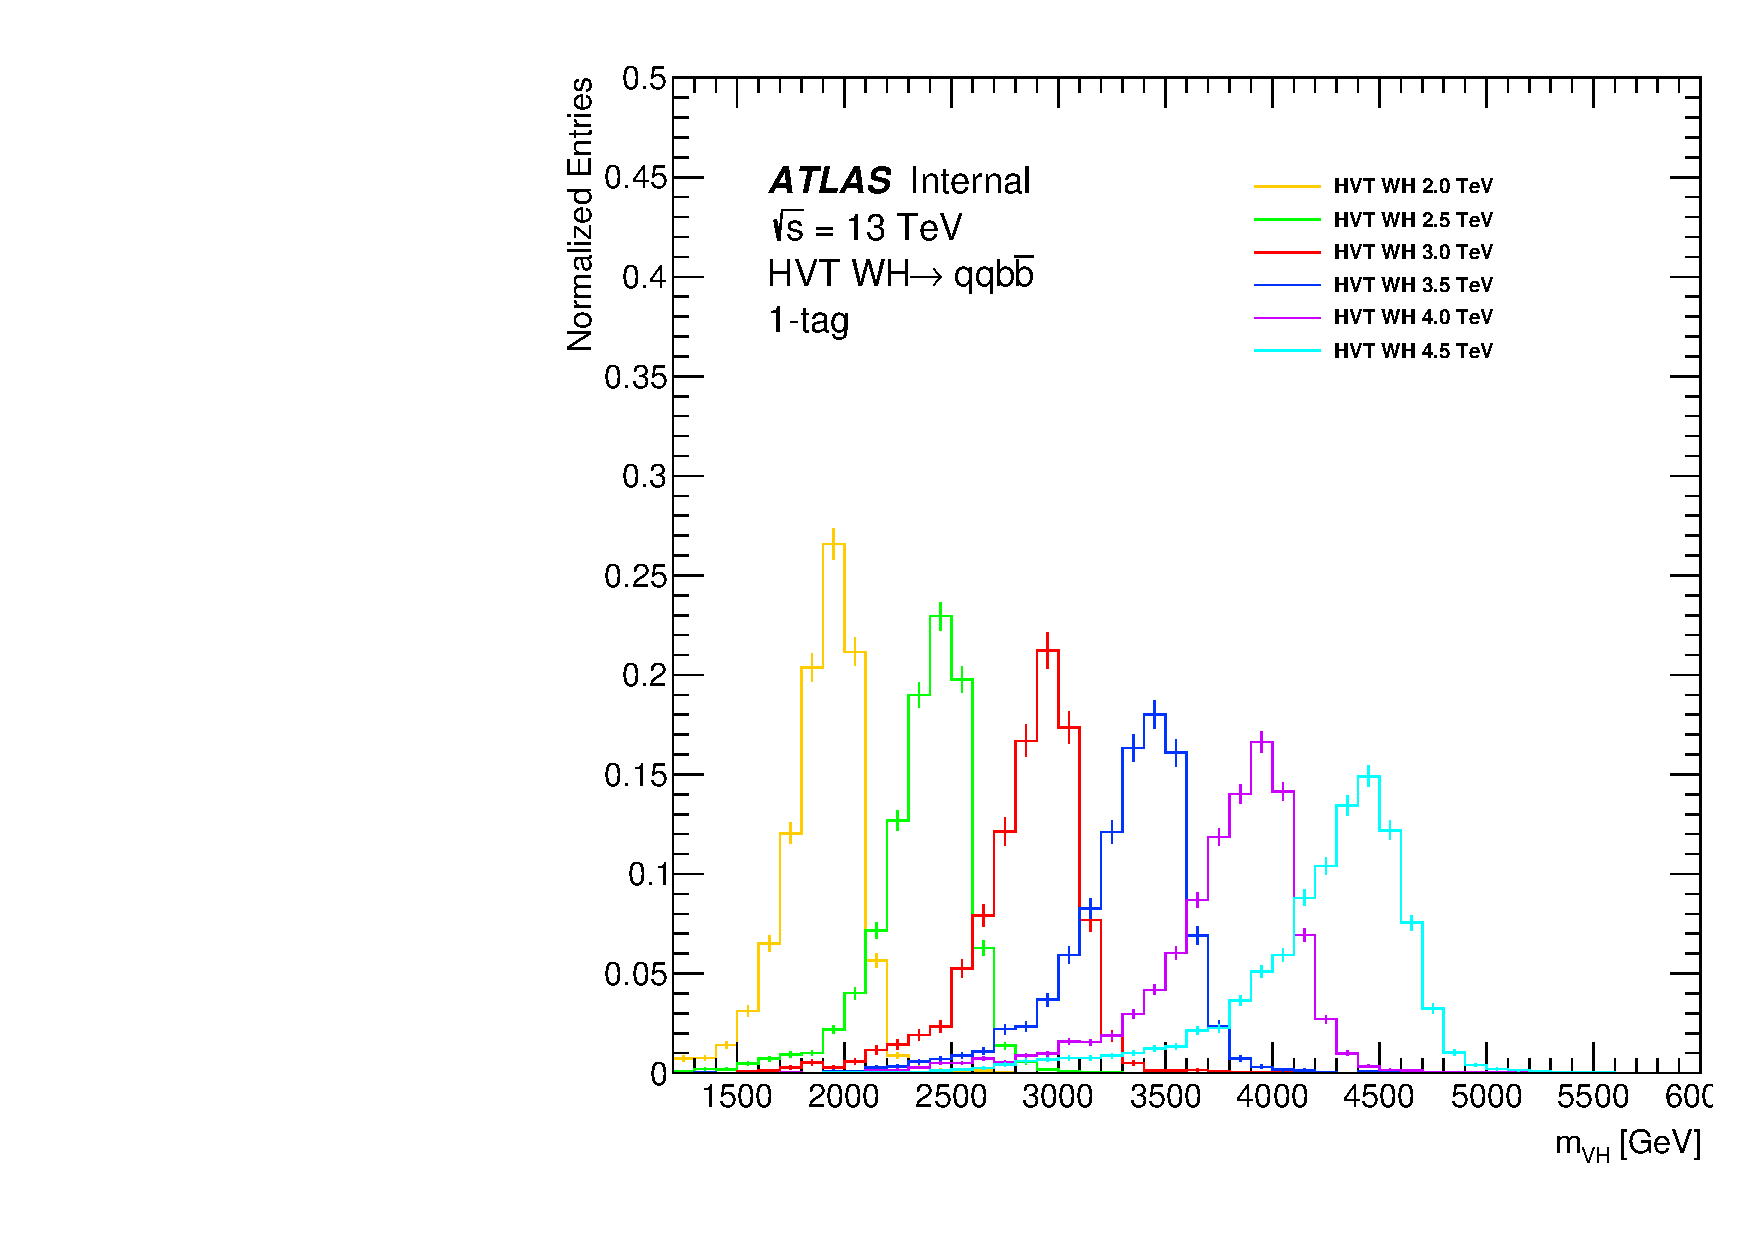
\includegraphics[width=0.49\textwidth]{VHqqbb_WH_1tag_SignalPeaks.pdf}
    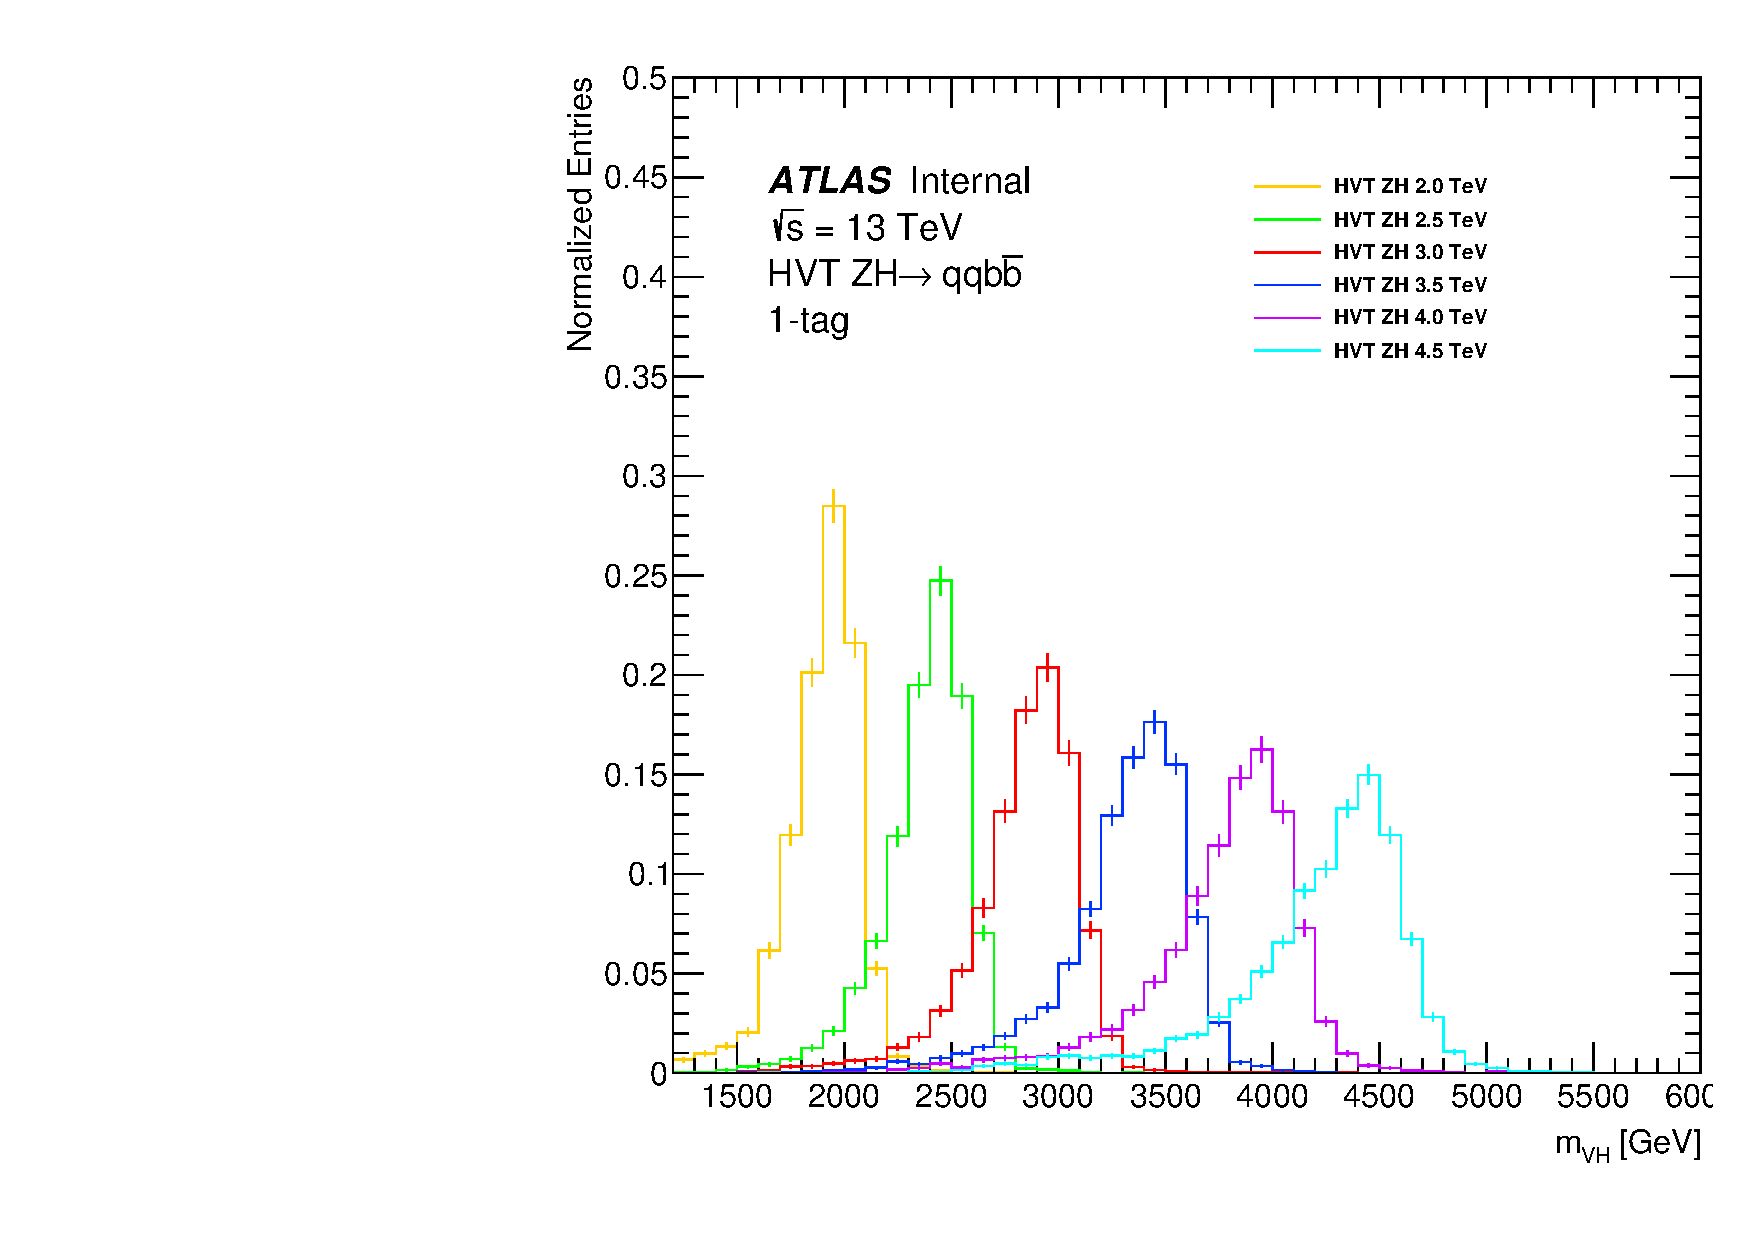
\includegraphics[width=0.49\textwidth]{VHqqbb_ZH_1tag_SignalPeaks.pdf} \\
    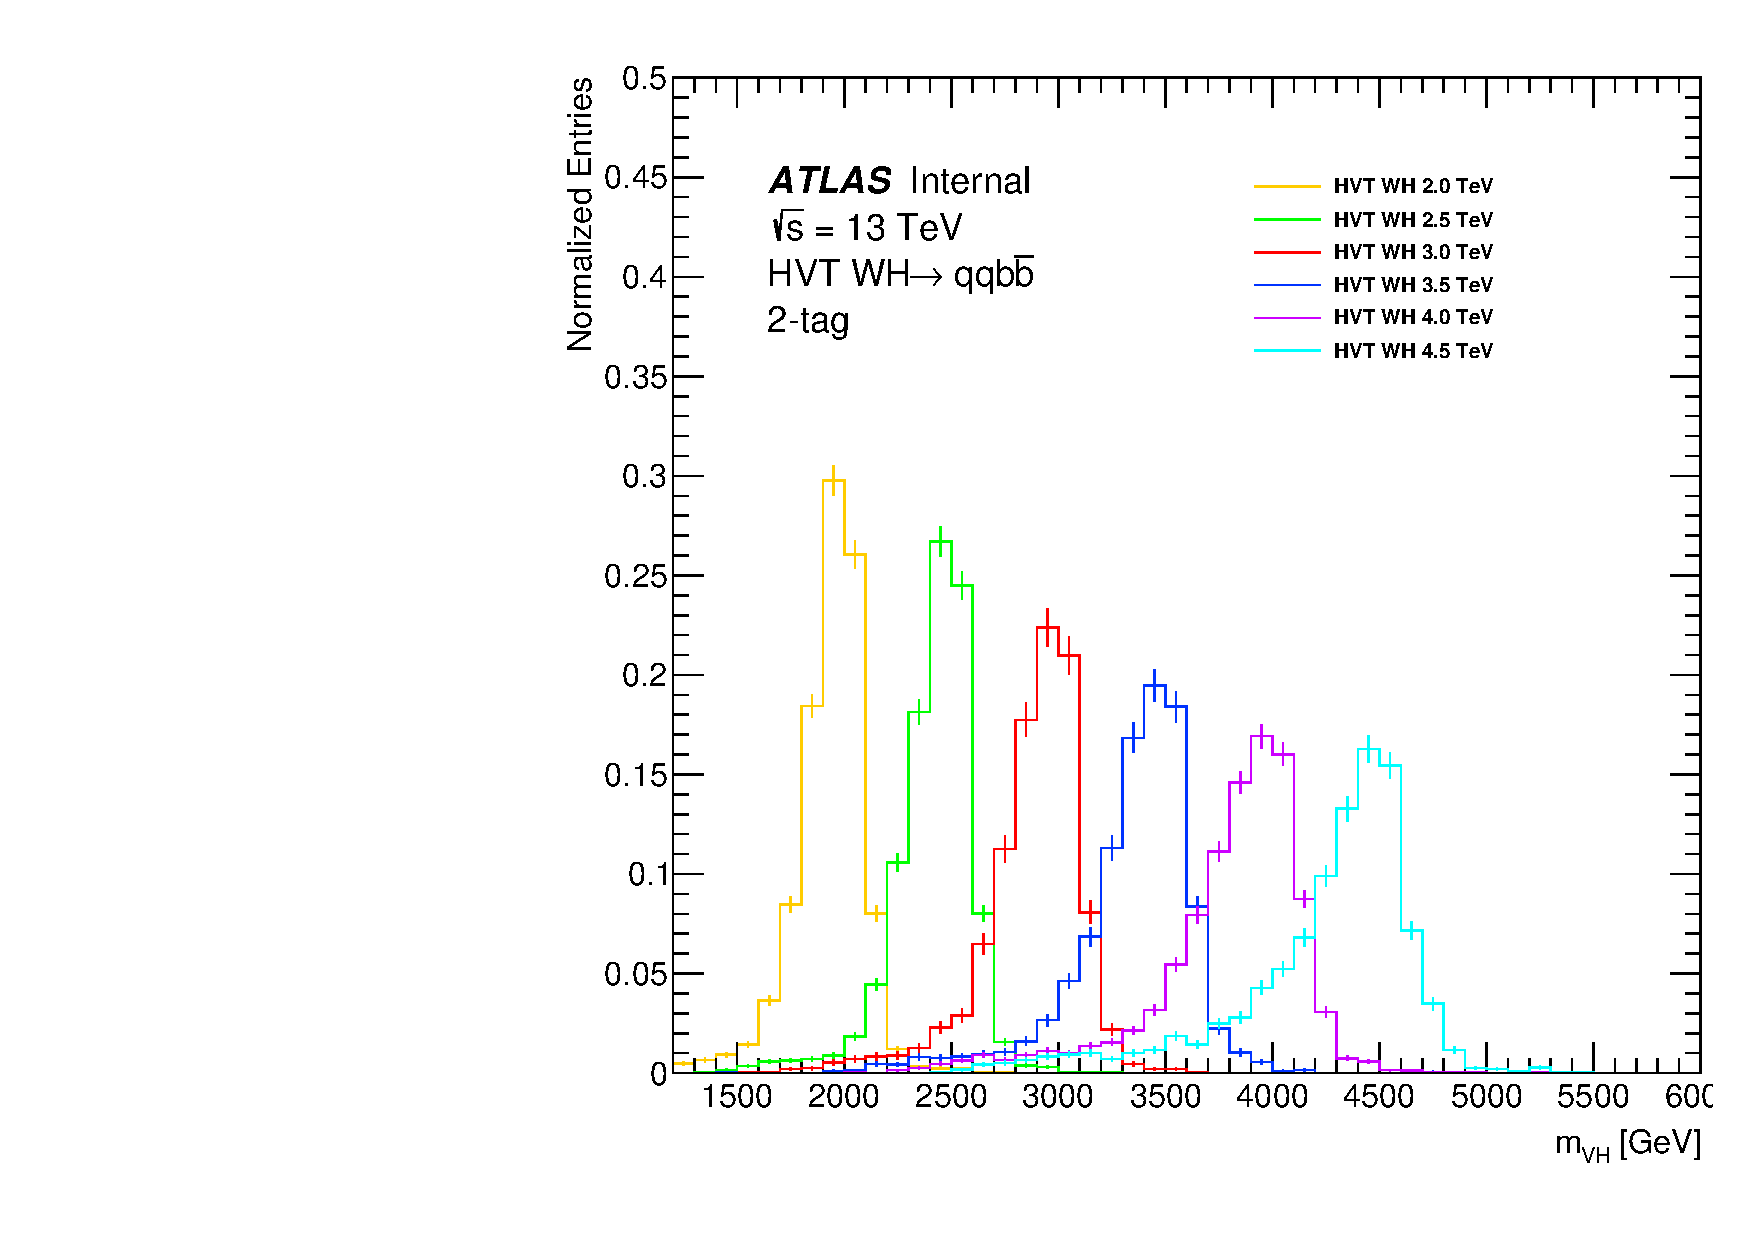
\includegraphics[width=0.49\textwidth]{VHqqbb_WH_2tag_SignalPeaks.pdf}
    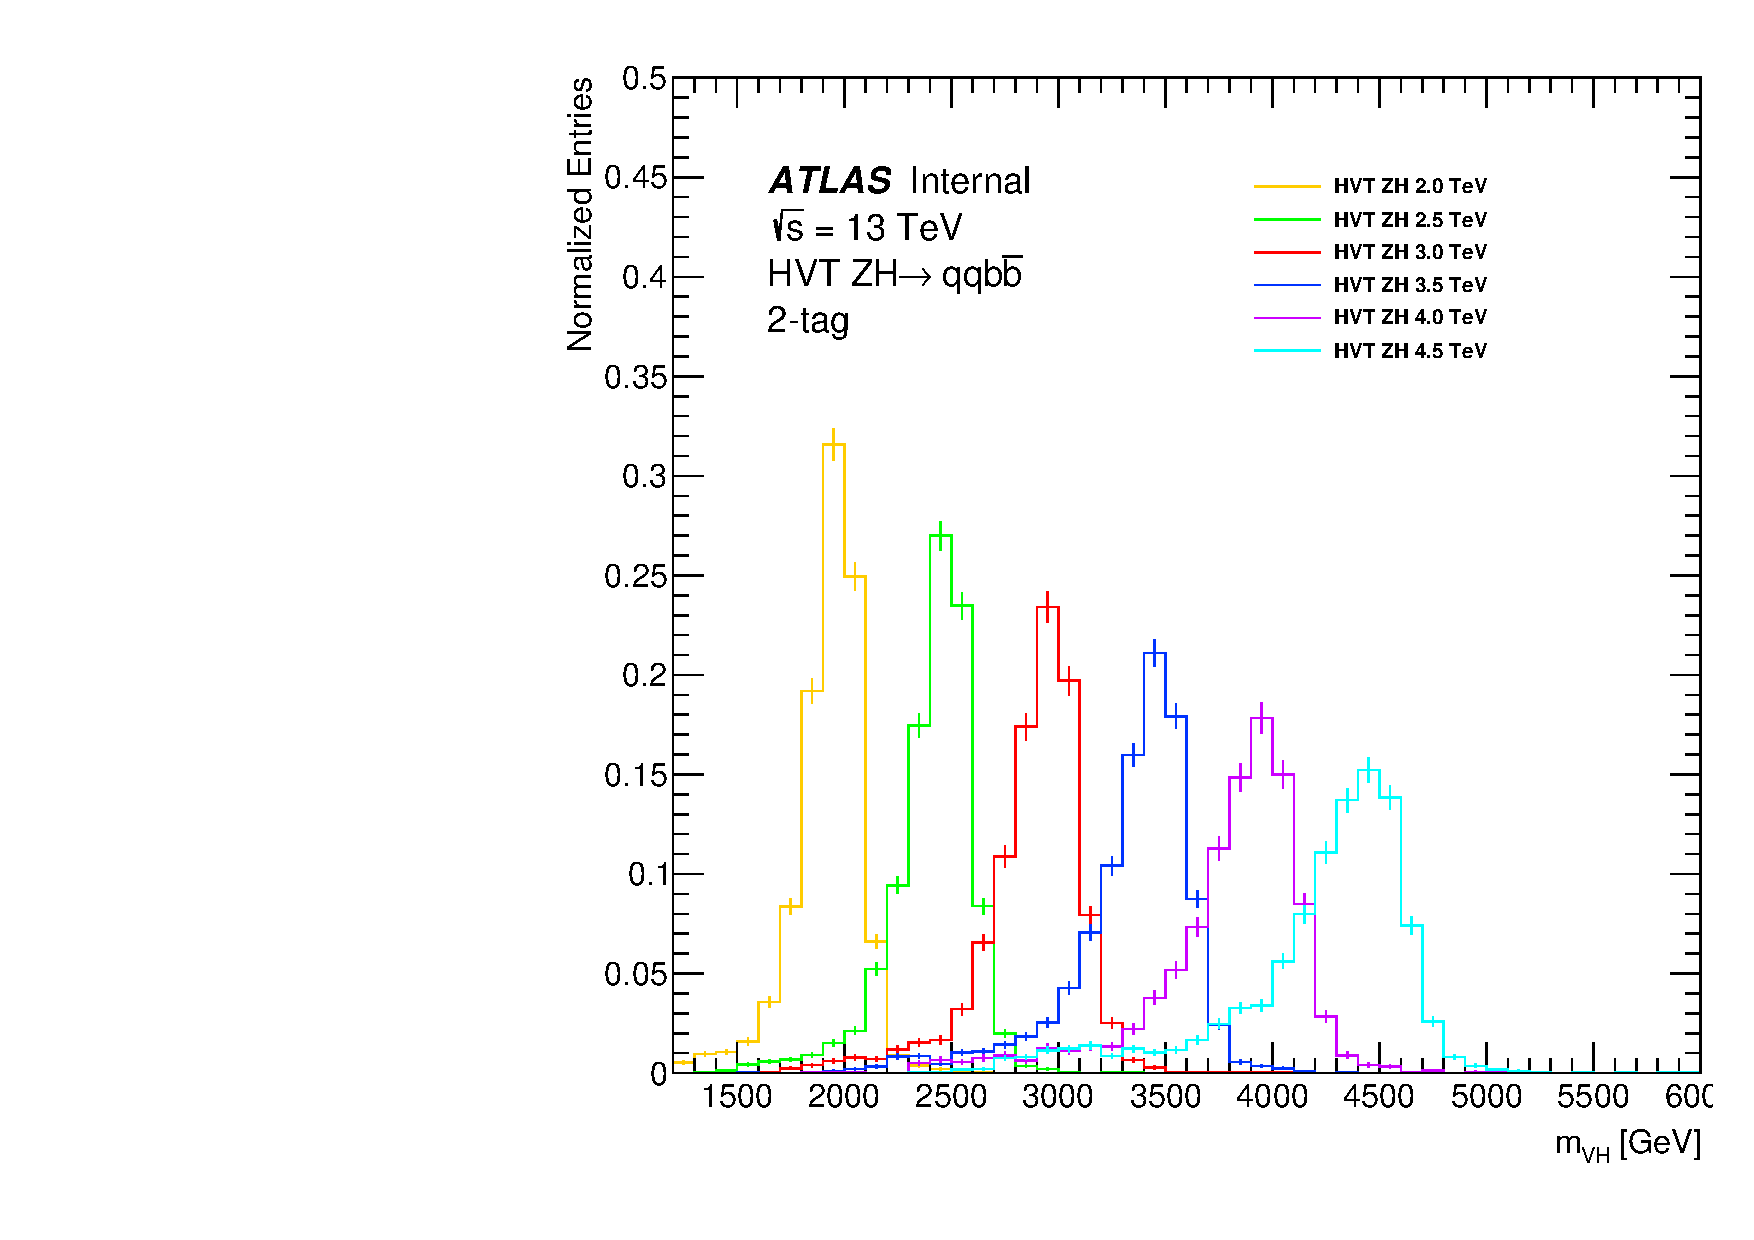
\includegraphics[width=0.49\textwidth]{VHqqbb_ZH_2tag_SignalPeaks.pdf}
\end{center}
\caption{Reconstructed dijet invariant mass distribution of $WH$ (left) and $ZH$ (right) signal MC samples, for selected resonance mass points, in 1-tag (top) and 2-tag (bottom) signal regions. The distributions are normalization to unity.}
\label{fig:signalMjj}
\end{figure}

\begin{table}[htbp!]
\normalsize
\centering
\begin{tabular}{c|c}
\hline
Cut & Description \\
\hline
EXOT3 & \ref{subsec:exot3} \\
\hline
GRL & See Section~\ref{subsec:data} \\
\hline
Event Cleaning & See Section~\ref{subsec:evtclean} \\
\hline
Trigger & See Section~\ref{subsec:trig} \\
\hline
$\geq 2$ large-R jets & $p_{T}>200$ GeV, $|\eta|<2.0$ \\
\hline
Leading large-R jet $p_{T}$ & $>500$ GeV \\
\hline
Dijet Mass (\mvh) & $>1.3$ TeV \\
\hline
Rapidity difference & $|\Delta y|<1.6$\\
\hline
\hline
V/H assignment & Heavier is H-candidate, lighter is V-candidate \\
\hline
W/Z tagging & mass window + $D_{2}$ + \ntrk \\
\hline
Higgs tagging & mass window + \ntrk \\
\hline
\end{tabular}
\caption{Summary of event selection.}
\label{tab:selection}
\end{table}

\begin{figure}[htbp!]
\begin{center}
\subfloat[]{%
    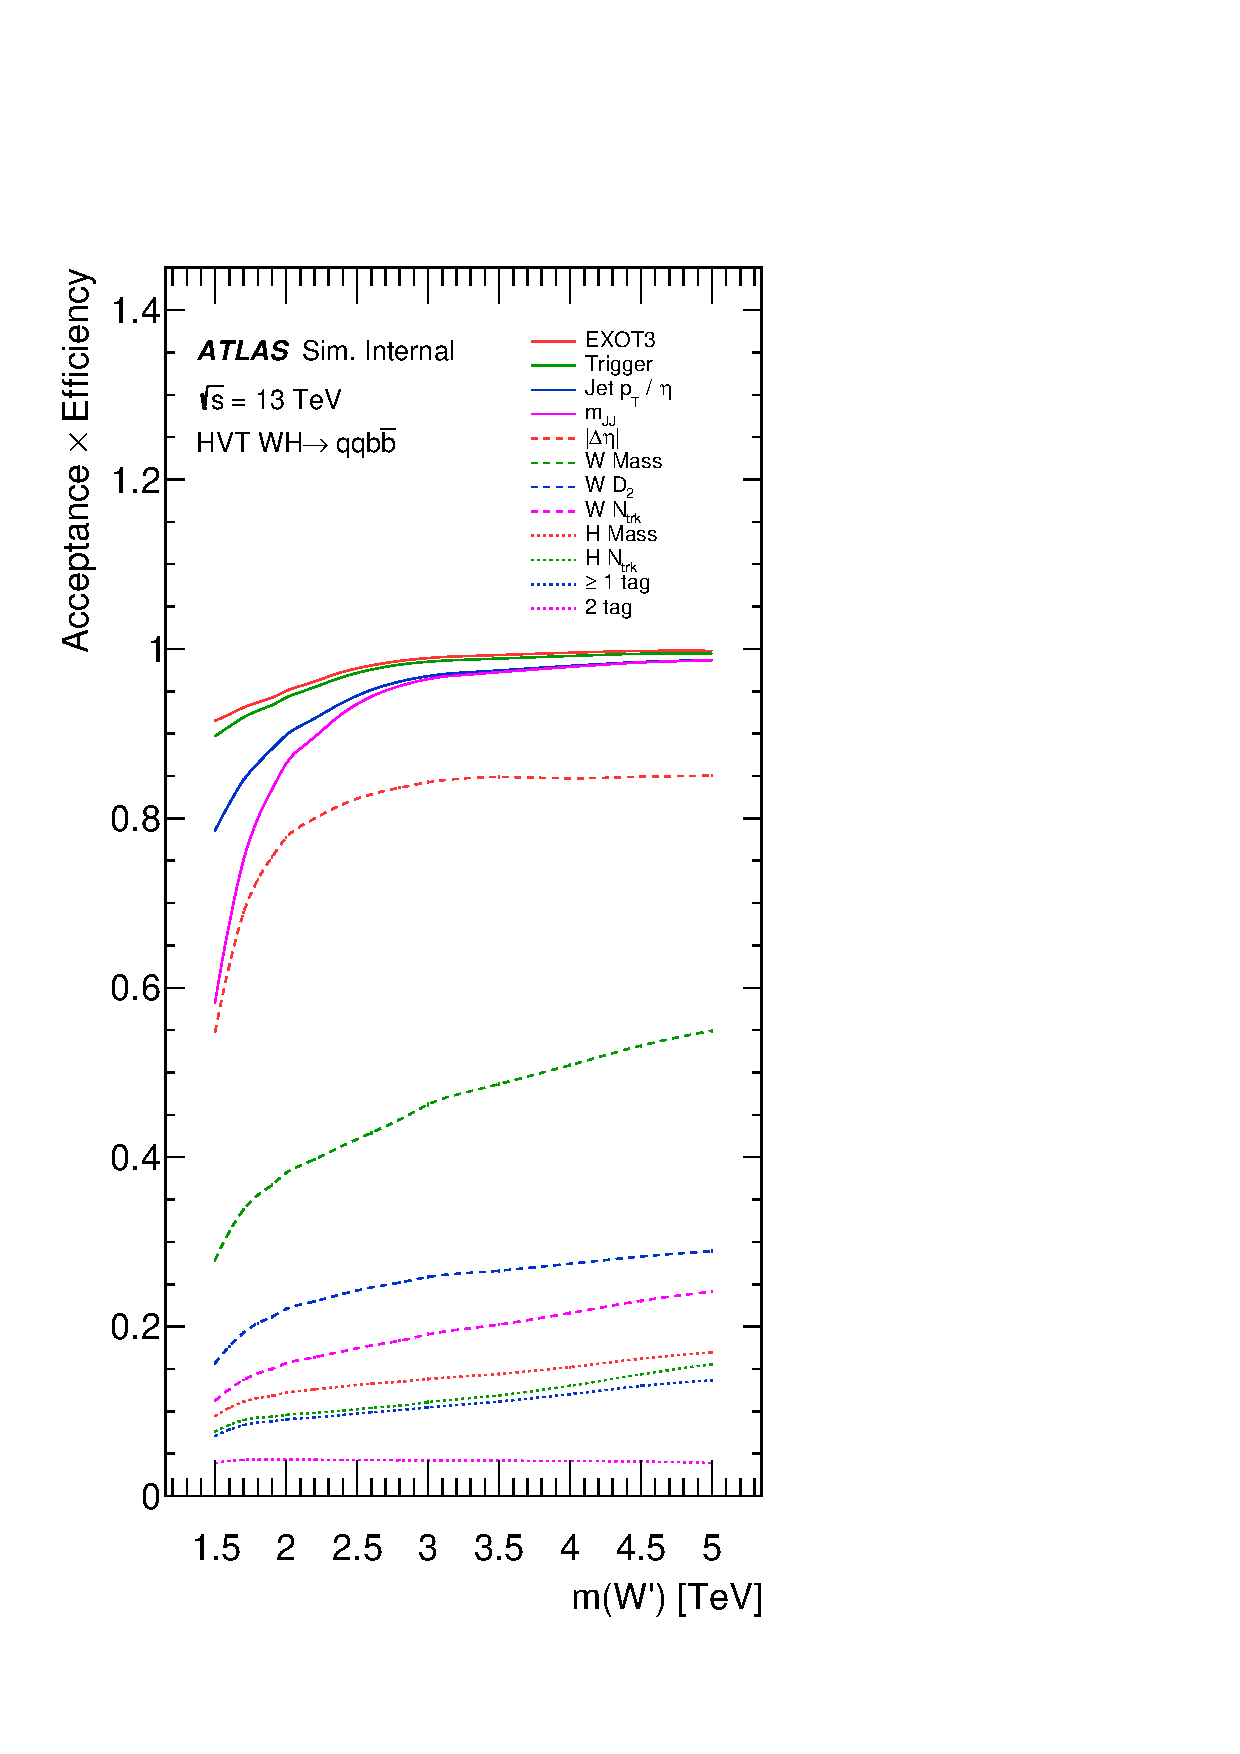
\includegraphics[width=0.49\textwidth]{VHqqbb_WH_Eff.pdf}
}
\subfloat[]{%
    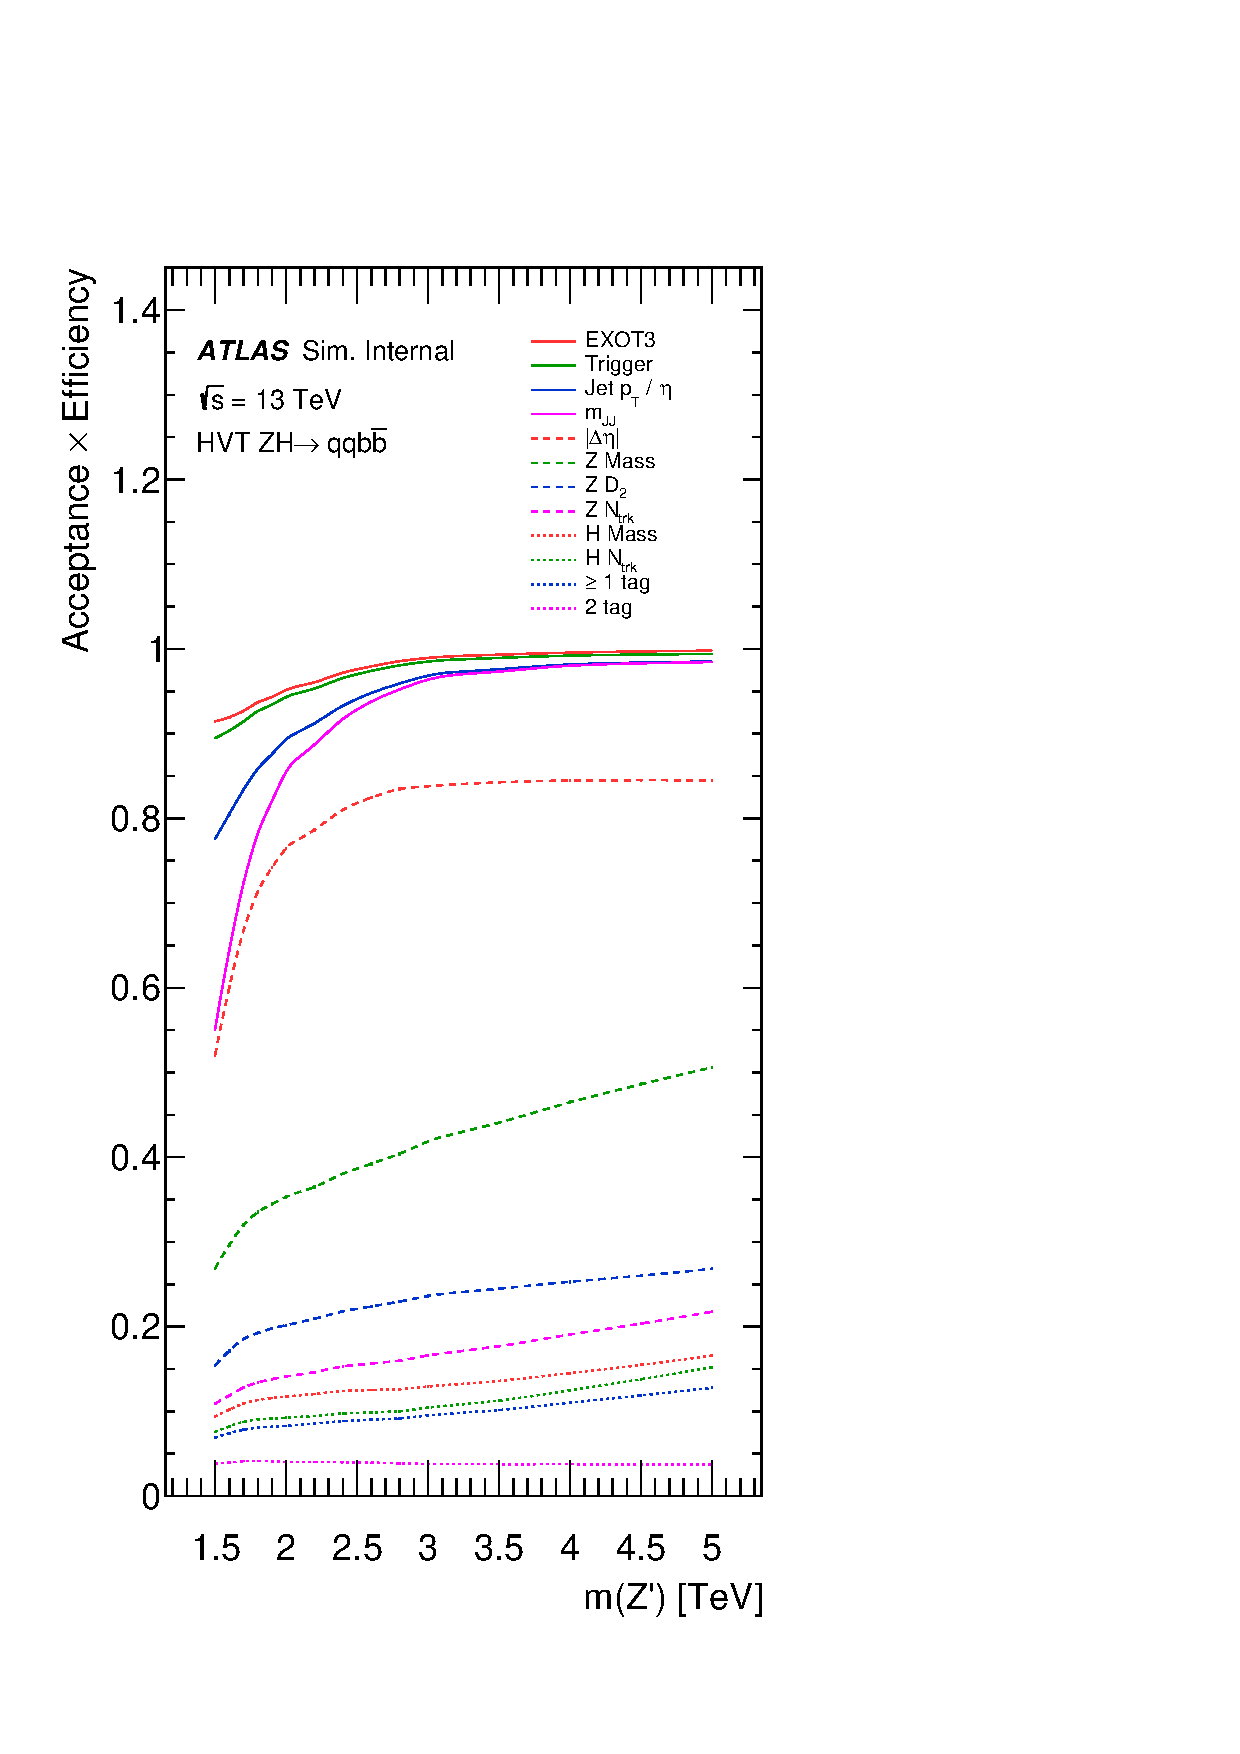
\includegraphics[width=0.49\textwidth]{VHqqbb_ZH_Eff.pdf}
}
\end{center}
\caption{Signal efficiency at various stages of the event selection as a function of resonance mass for the WH (a) and ZH (b) selections (applied to the corresponding signal sample).
    Each cut is added to the selection of the previous cut in sequence, from top to bottom.
}
\label{fig:effVH}
\end{figure}

\begin{figure}[htbp!]
    \begin{center}
        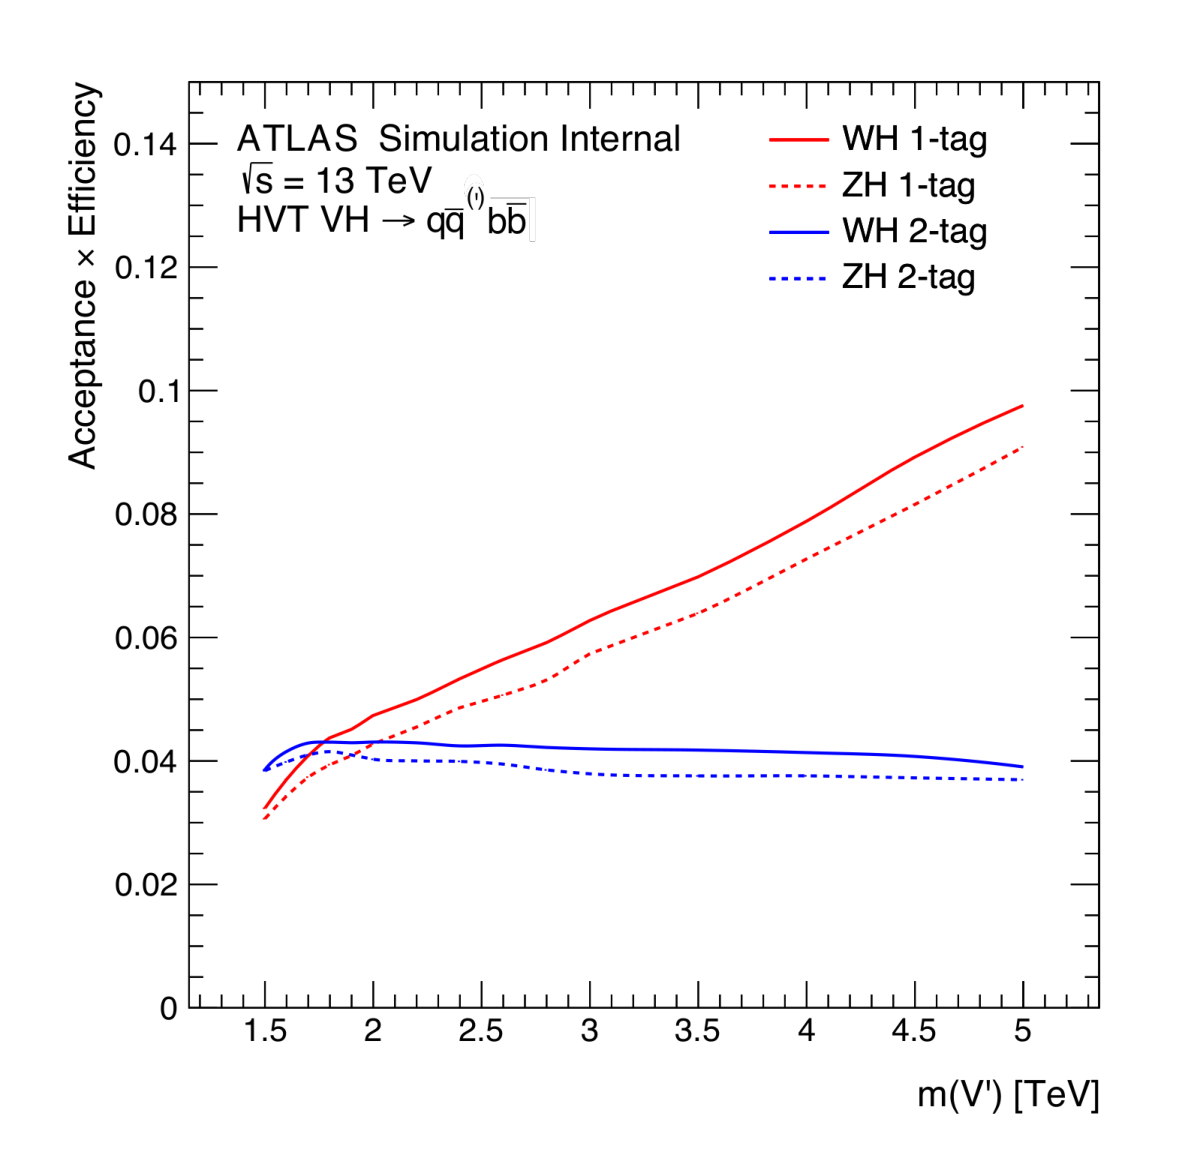
\includegraphics[width=0.7\textwidth]{VHqqbb_SignalEffChannels.pdf}
    \end{center}
    \caption{Signal efficiency as function of resonance mass for both $WH$ and $ZH$ signal processes, 1-tag and 2-tag channels.}
    \label{fig:effcurve}
\end{figure}

\begin{table}[htbp!]
    \normalsize
    \centering
    \begin{tabular}{c||ccc}
        Cut Name & $\sum{\mathrm{weights}}$ & Cut Efficiency [\%] & Cumulative Efficiency [\%] \\ \hline
        Generated & 105000 & -- & --\\ \hline
        EXOT3 & 99463 & 94.7 & 94.7\\ \hline
        Jet/Event Cleaning & 99112 & 99.6 & 94.4\\ \hline
        Trigger & 98662 & 99.5 & 94.0\\ \hline
        Jet $p_{T}$ / $\eta$ & 94114 & 95.4 & 89.6\\ \hline
        $m_{\mathrm{JJ}}$ & 90451 & 96.1 & 86.1\\ \hline
        $|\Delta y_{12}|$ & 81206 & 89.8 & 77.3\\ \hline
        W Mass & 39540 & 48.7 & 37.7\\ \hline
        W $D_{2}$ & 22755 & 57.5 & 21.7\\ \hline
        W $n_{\mathrm{trk}}$ & 16114 & 70.8 & 15.3\\ \hline
        H Mass & 12569 & 78.0 & 12.0\\ \hline
        H $n_{\mathrm{trk}}$ & 9867 & 78.5 & 9.4\\ \hline
        $\geq$ 1-tag & 9303 & 94.3 & 8.9\\ \hline
        2-tag & 4523 & 48.6 & 4.3\\ \hline
    \end{tabular}
    \caption{Cutflow for the 2.0 TeV WH signal sample. Where appropriate, $b$-tagging and boson tagging scale factors are included. }
    \label{tab:wh_2TeV_cutflow}
\end{table}

\begin{table}[htbp!]
    \normalsize
    \centering
    \begin{tabular}{c||ccc}
        Cut Name & $\sum{\mathrm{weights}}$ & Cut Efficiency [\%] & Cumulative Efficiency [\%] \\ \hline
        Generated & 75000 & -- & --\\ \hline
        EXOT3 & 74713 & 99.6 & 99.6\\ \hline
        Jet/Event Cleaning & 74463 & 99.7 & 99.3\\ \hline
        Trigger & 74451 & 100.0 & 99.3\\ \hline
        Jet $p_{T}$ / $\eta$ & 73644 & 98.9 & 98.2\\ \hline
        $m_{\mathrm{JJ}}$ & 73550 & 99.9 & 98.1\\ \hline
        $|\Delta y_{12}|$ & 63393 & 86.2 & 84.5\\ \hline
        Z Mass & 34892 & 55.0 & 46.5\\ \hline
        Z $D_{2}$ & 18830 & 54.0 & 25.1\\ \hline
        Z $n_{\mathrm{trk}}$ & 14133 & 75.1 & 18.8\\ \hline
        H Mass & 10752 & 76.1 & 14.3\\ \hline
        H $n_{\mathrm{trk}}$ & 9239 & 85.9 & 12.3\\ \hline
        $\geq$ 1-tag & 8151 & 88.2 & 10.9\\ \hline
        2-tag & 2807 & 34.4 & 3.7\\ \hline
    \end{tabular}
    \caption{Cutflow for the 4.0 TeV ZH signal sample. }
    \label{tab:zh_4TeV_cutflow}
\end{table}

\begin{figure}[htbp!]
\begin{center}
    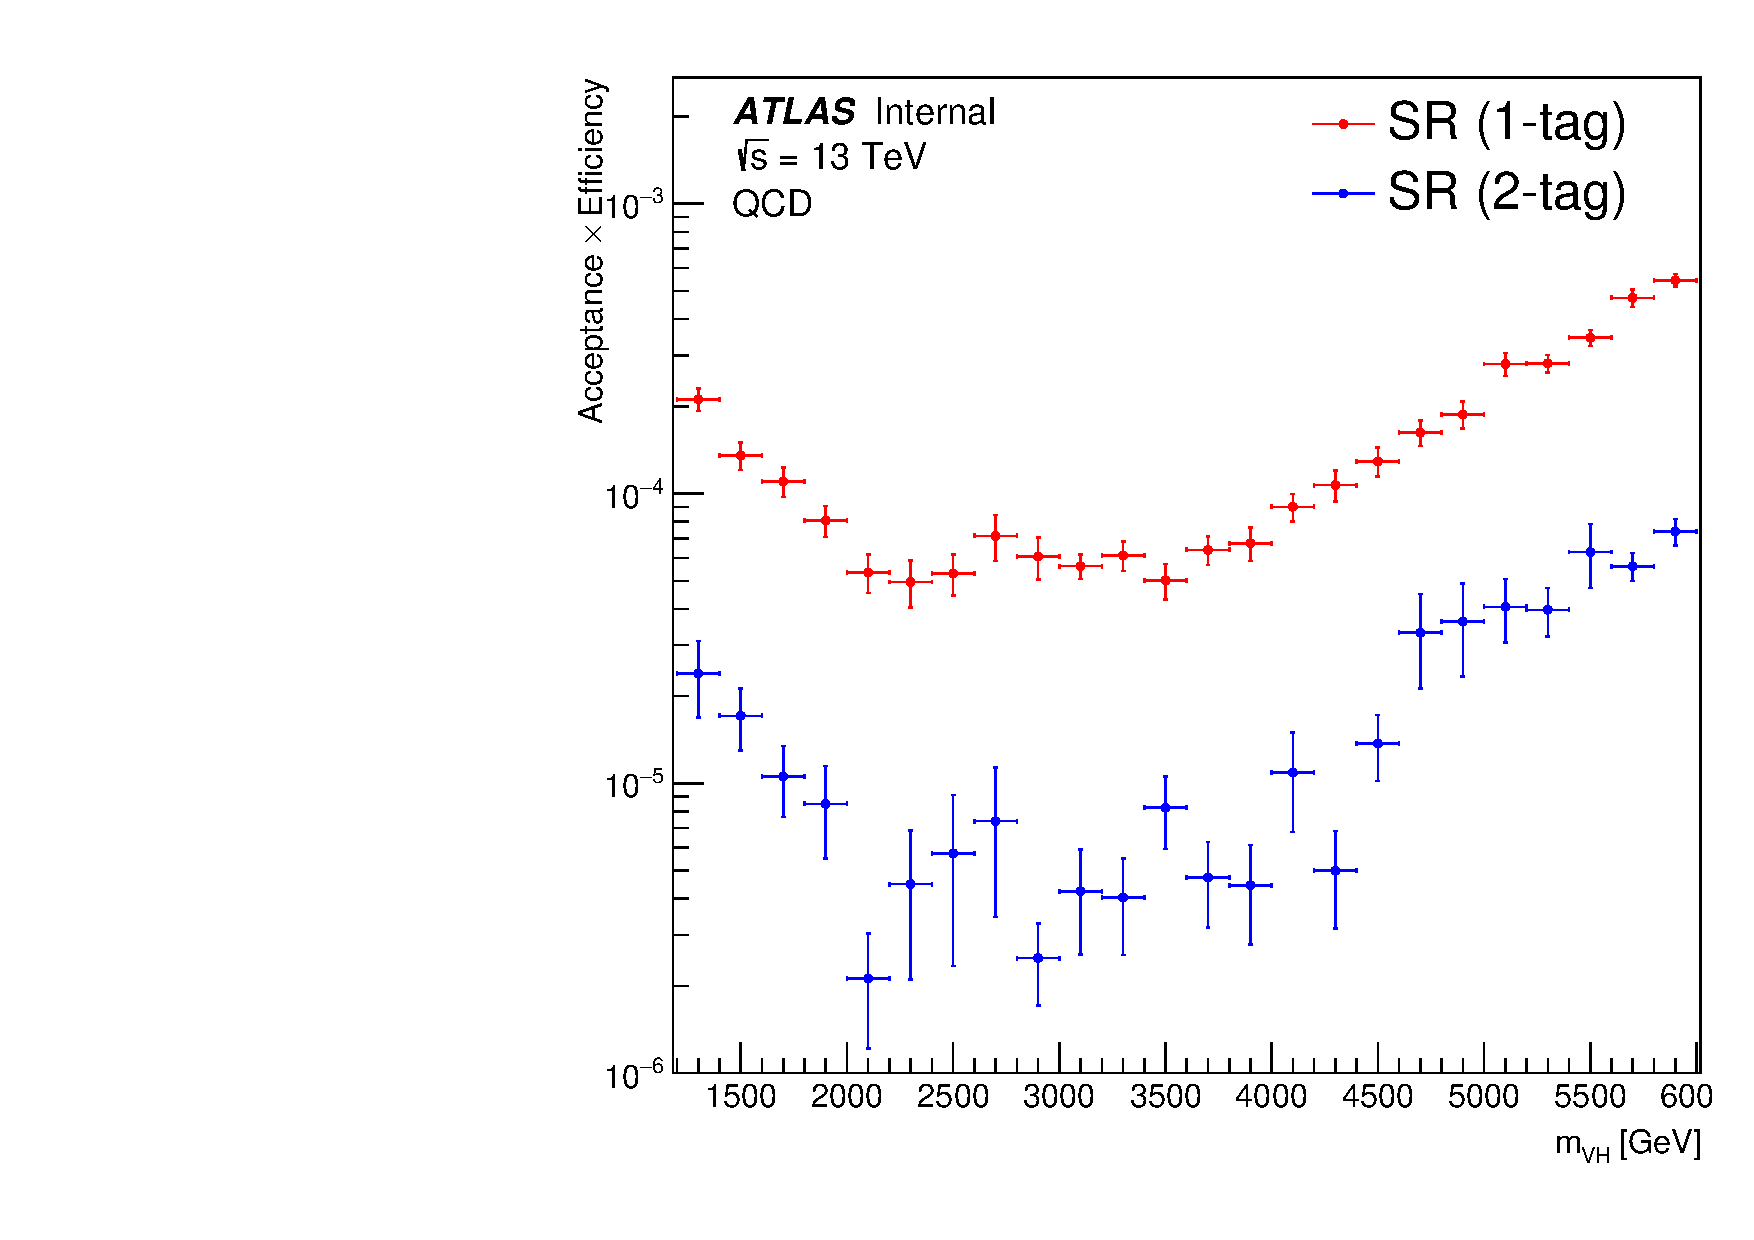
\includegraphics[width=0.49\textwidth]{PlotVHqqbbBkgRejection_dijet.pdf} \\
    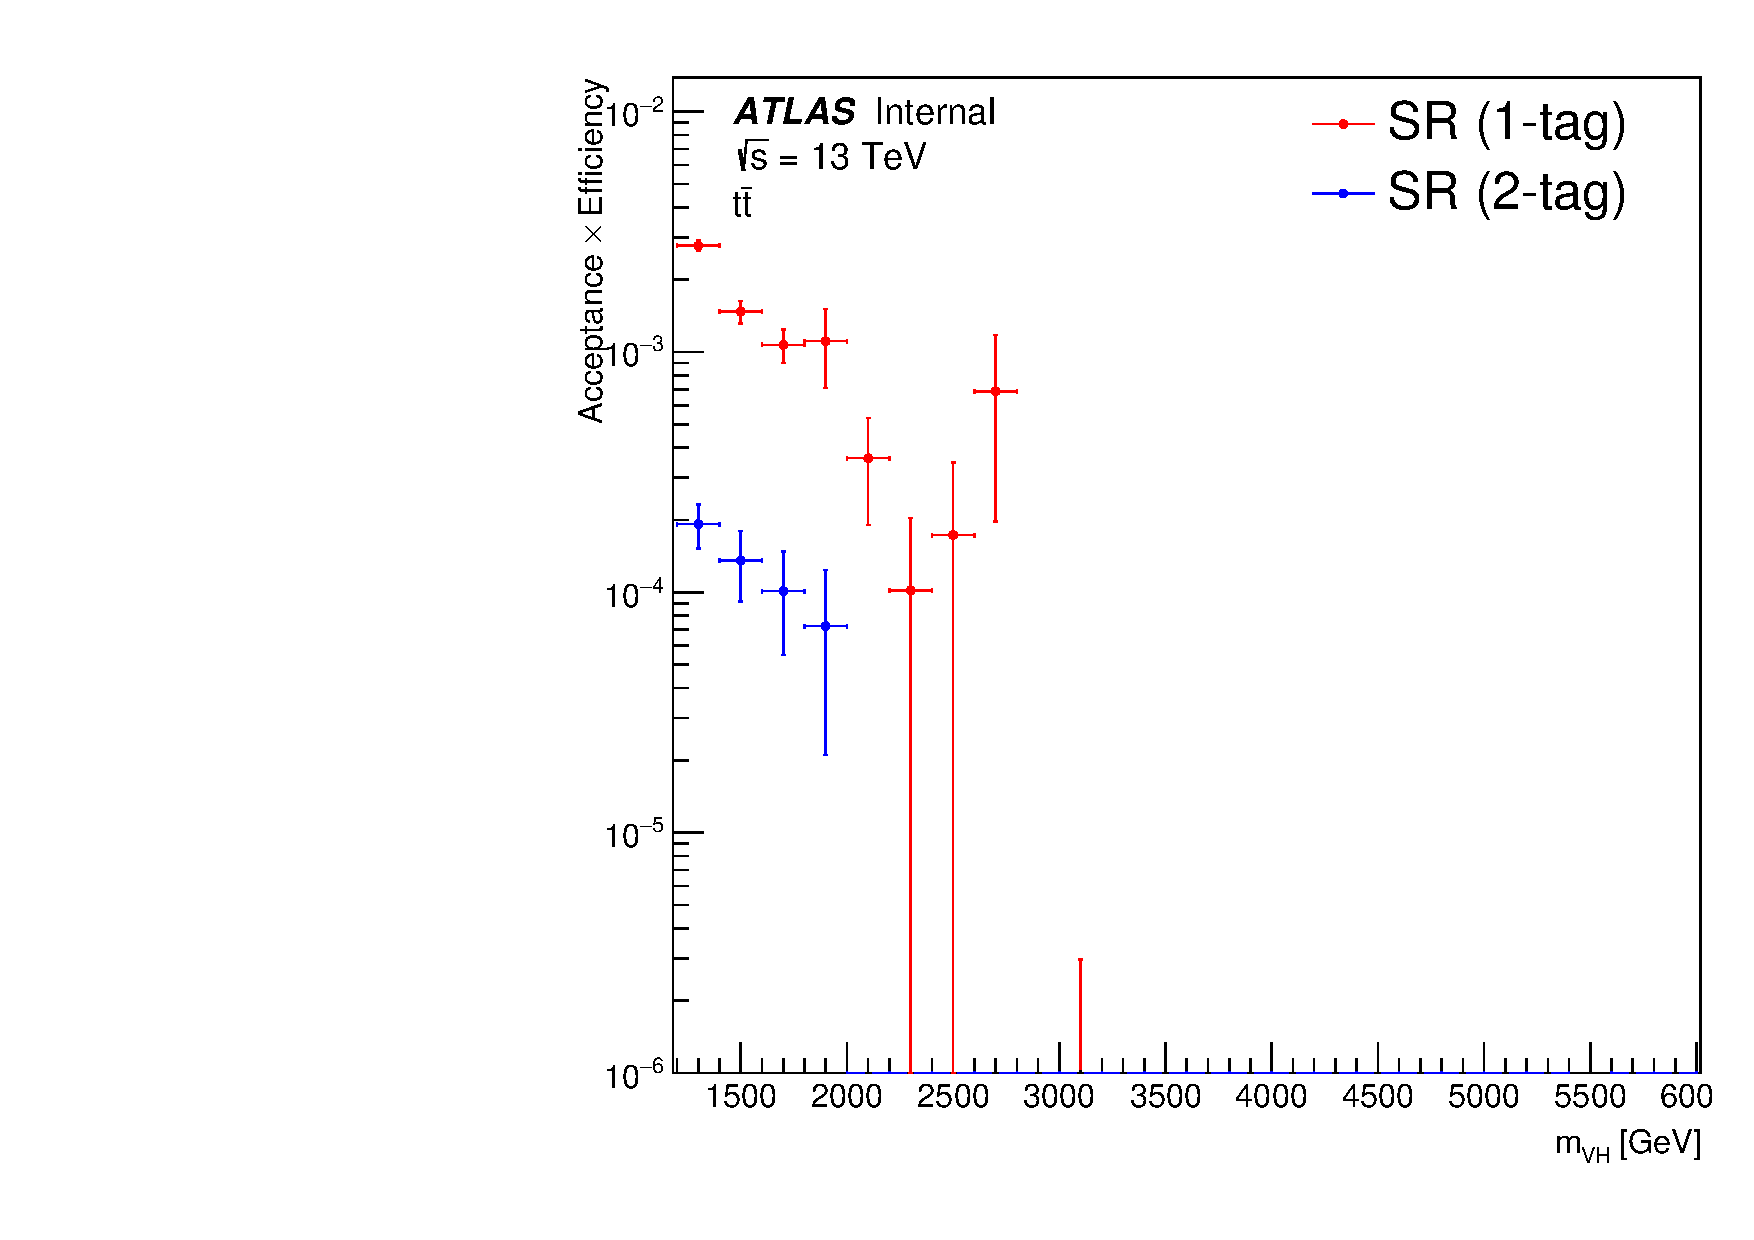
\includegraphics[width=0.49\textwidth]{PlotVHqqbbBkgRejection_ttbar.pdf}
    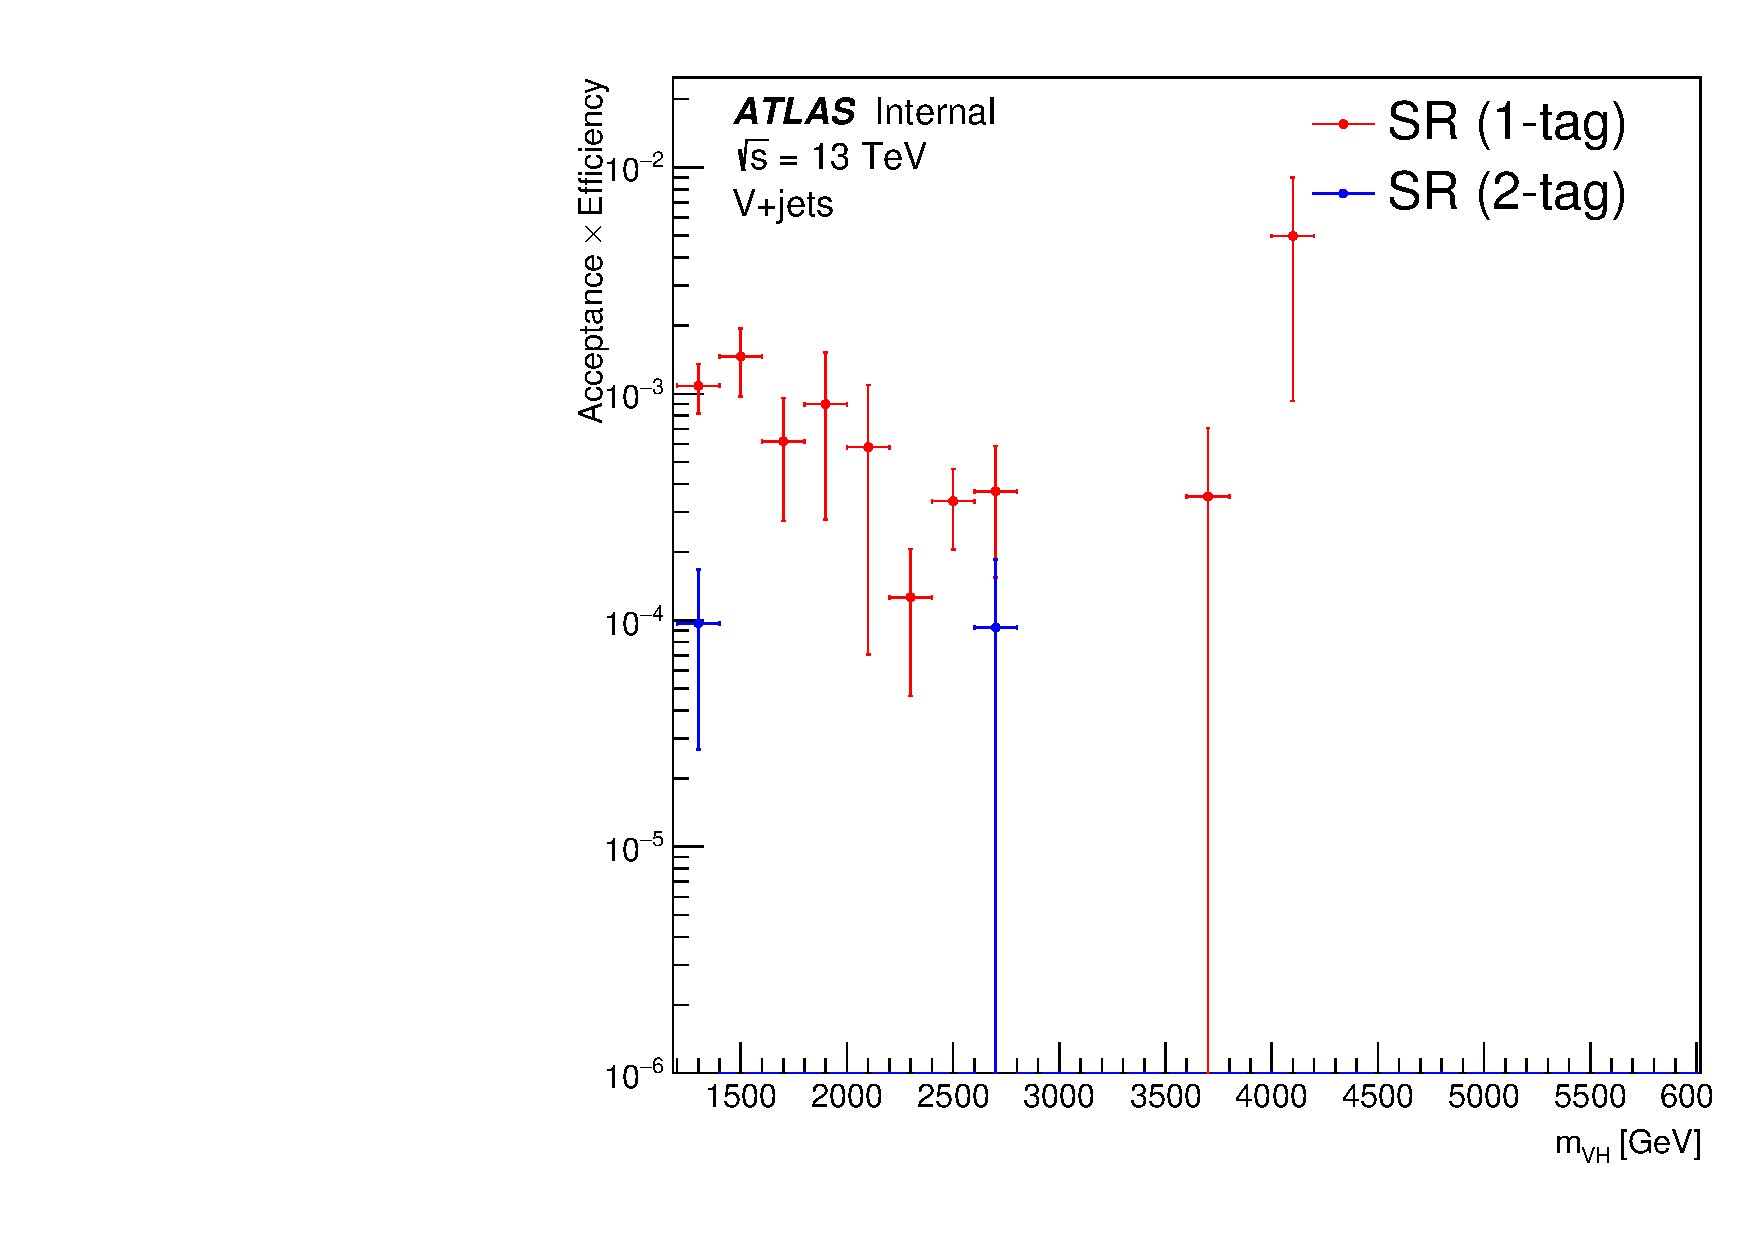
\includegraphics[width=0.49\textwidth]{PlotVHqqbbBkgRejection_vjets.pdf}
\end{center}
\caption{Background efficiencies in the signal regions for dijet, $t\bar{t}$ and $V$+jets MC. The 1-tag and 2-tag regions correspond to the combined $V=W,Z$ signal regions. The $t\bar{t}$ and $V$+jets efficiency predictions at high \mvh\ are hampered by lack of MC statistics.}
\label{fig:effBkg}
\end{figure}


\section{Background Estimation}
\label{sec:background}
%TODO: footnote defining 'kinematic'
The primary goal of the background estimation is to provide a prediction of the normalization and shape of the combined QCD, $t\bar{t}$, and $V$+jets backgrounds in the 1-tag and 2-tag signal regions (SR).
The variable of most interest is the invariant mass of the combined candidate VH system (\mvh).
However, a more complete model of event kinematics is pursued in order to produce comparisons of additional kinematic variables to further validate the complete background description.

The dominant contribution to the background comes from approximately 90\% QCD events.
The $t\bar{t}$ background is predicted to contribute approximately 10\% to all SRs, and a small contribution of less than 1\% from V+jets is also present.
Other backgrounds such as diboson $WW\ /\ WZ\ /\ ZZ$ are expected to be present but negligible and are therefore not considered.
Modelling the background directly with MC is hampered for two primary reasons: (1) the QCD MC provides only a LO prediction and (2) the high background rejection of the SR selection severely limits the available MC statistics.
Therefore a data-driven method is used to extract the background estimation.

Any approach chosen to produce a background estimation needs to mitigate two fundamental competing factors, namely (1) the potential use of high statistics samples from a control region to reduce statistical and high-mass extrapolation uncertainties, and orthogonally (2) the reduction of systematic uncertainties (but increase in statistical uncertainty) by estimating backgrounds as close as possible to (or directly in) the SRs.

\begin{figure}[htbp!]
\begin{center}
    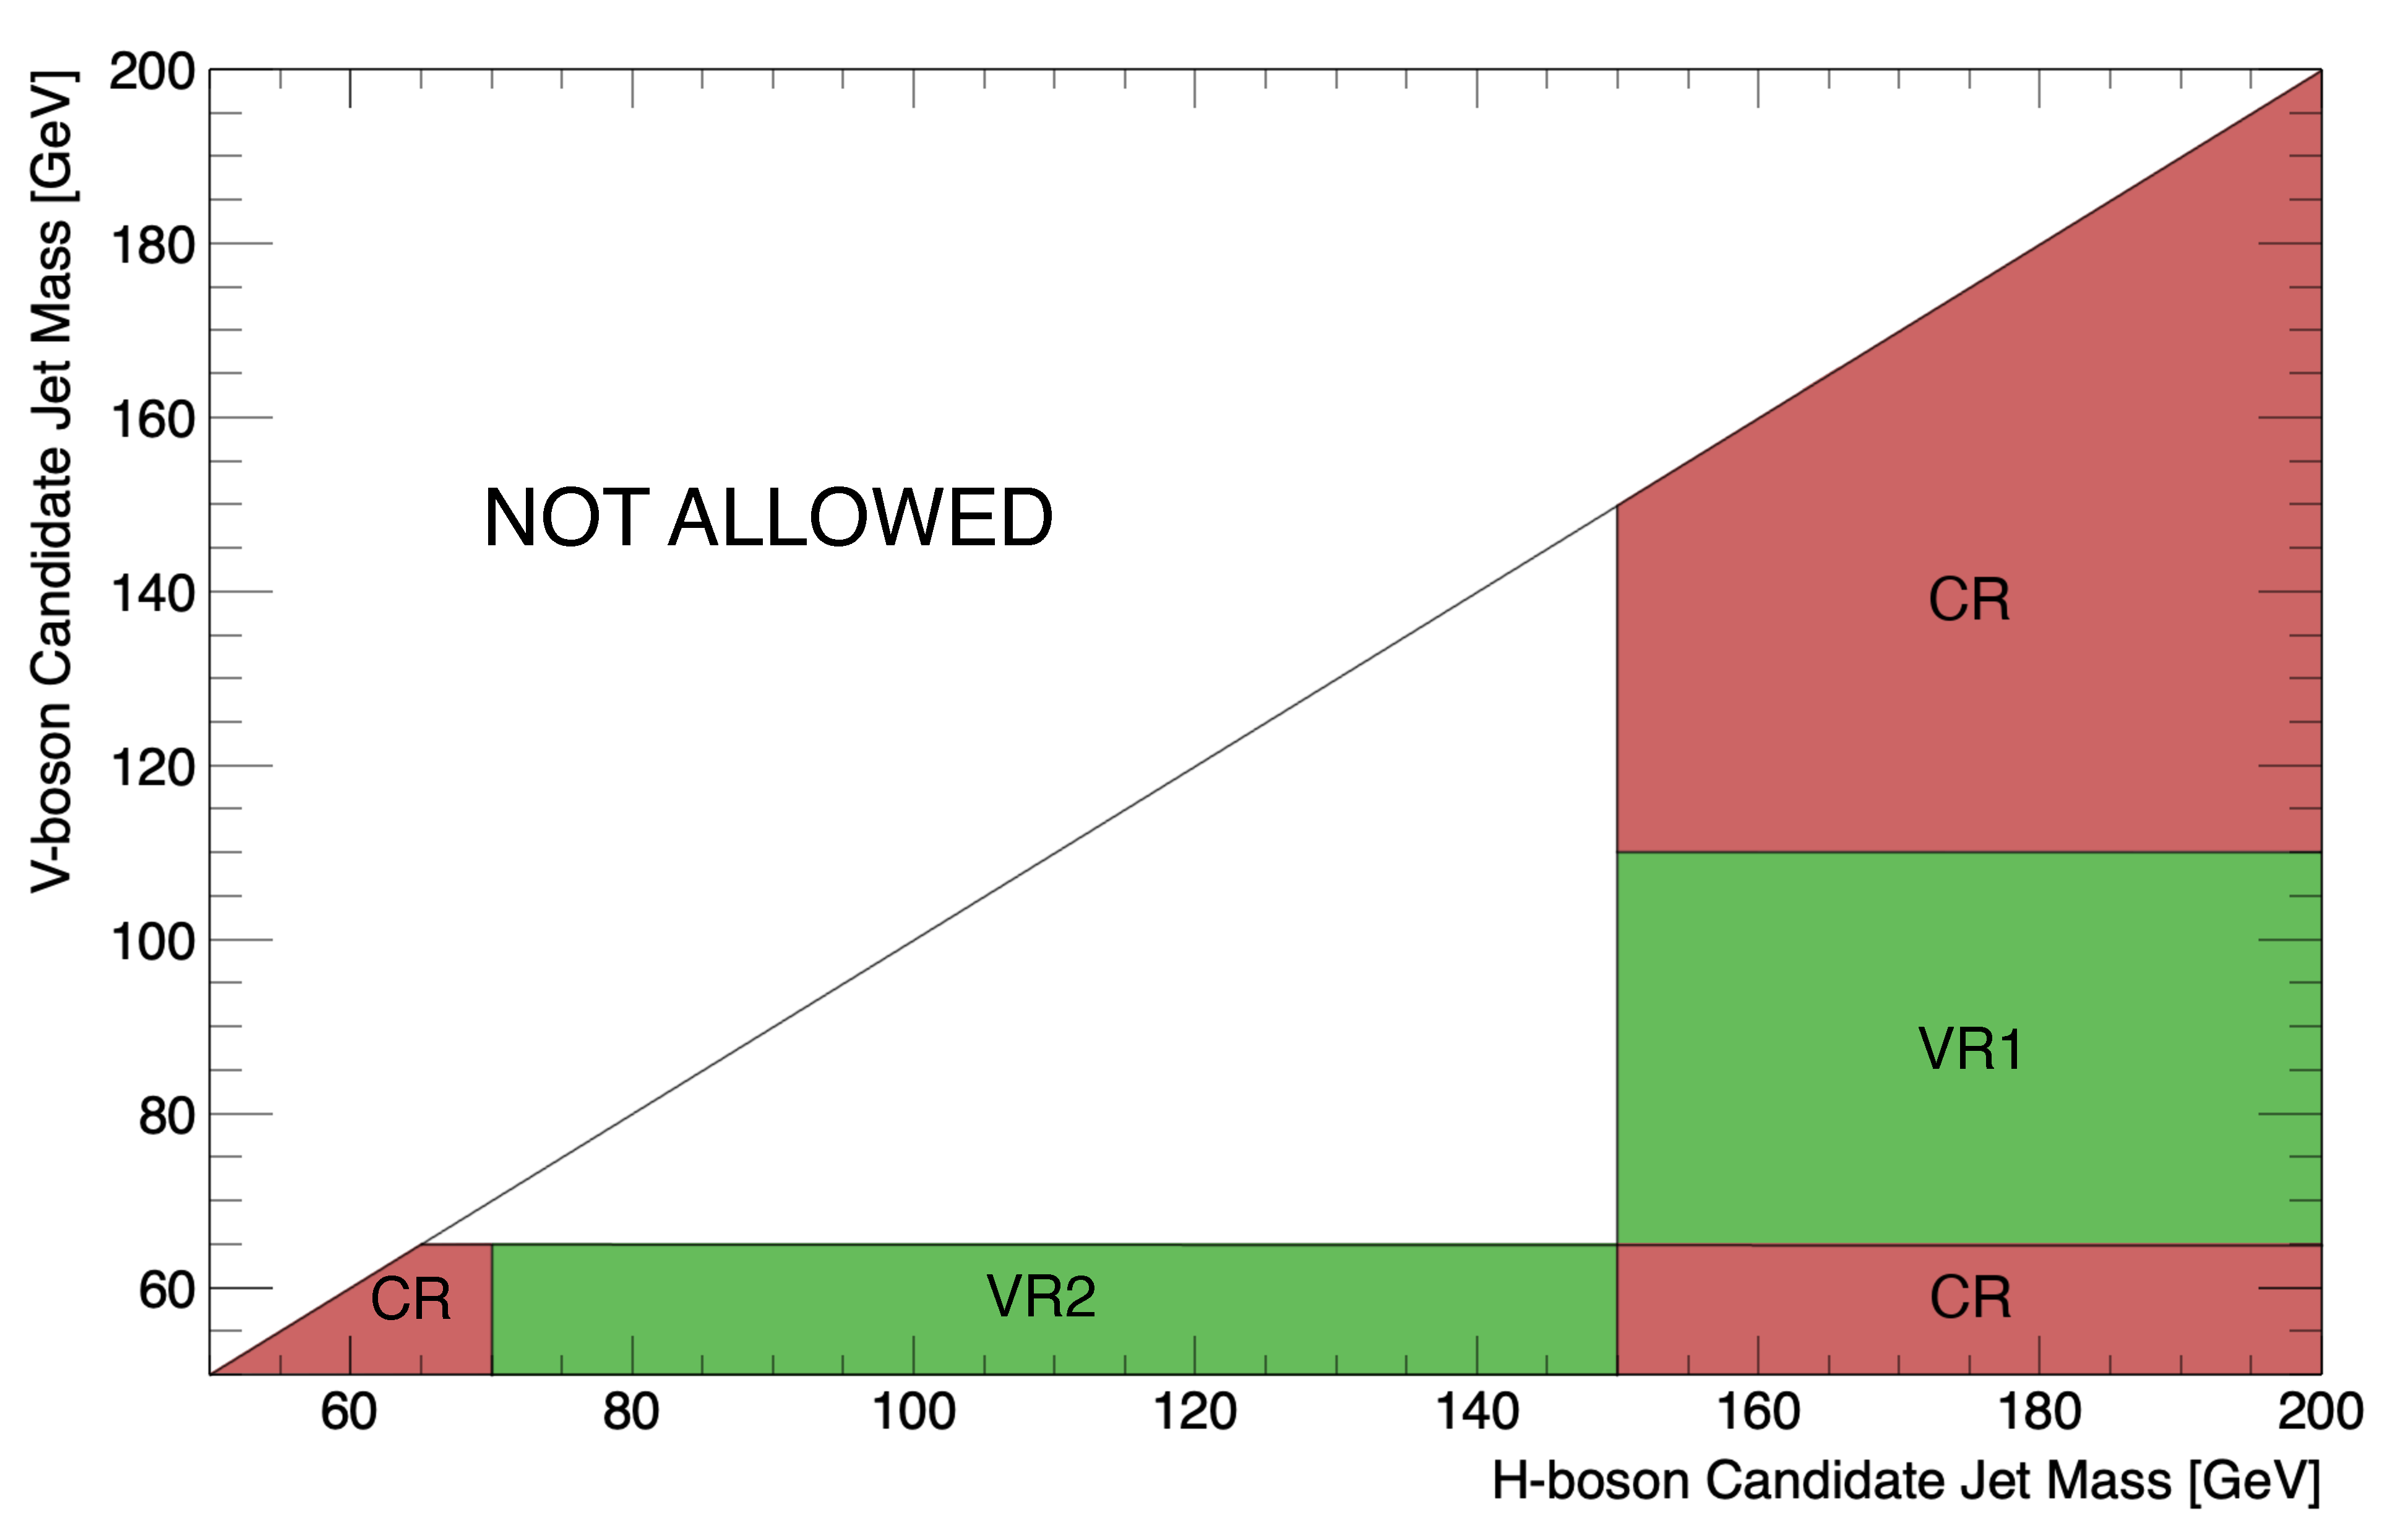
\includegraphics[width=0.75\textwidth]{CR_VR_Plane_Plot.pdf}
\end{center}
\caption{Illustration of the control and validation regions used to derive the background estimations. Signal Regions are not shown as they are not defined by a fixed mass window. The upper left region of the plane is not allowed due to the restriction that $m_V < m_H$.}
\label{fig:crvr_plane}
\end{figure}

As a result of these competing factors, multiple background estimation techniques have been developed and studied during previous iterations of this analysis:
\begin{itemize}
    \itemsep0em 
\item \textbf{0-Tag Based Re-Weighting Estimation:}
    Events with 0 b-tags are used as a model for the corresponding 1/2-tag selection.
    A control region is used to derive a kinematic re-weighting to facilitate the transformation from the 0-tag events to predictions for the corresponding 1/2-tag region.
    A re-weighting is needed, beyond a simple normalization scale factor, due to the sculpting of the jet \pt\ distribution that occurs after applying b-tagging requirements.
    The variables used in the re-weighting are those relevant to the b-tagging, and they are described in more detail in Section ~\ref{sec:bkg-reweighting}.
    The quality of this prediction is estimated by cross-checking the method with a set of validation regions which are orthogonal to the signal regions.

\item \textbf{High Mass SB Based Estimation:}
    Events with a Higgs candidate in the high mass sideband are used as a model for QCD.
    The 0 b-tag events are used for validation and/or to derive a normalization scale factor from the high mass sideband to the SRs.

\item \textbf{Direct Fit based Estimation:}
    The events in the SR are fit directly with a parameterized function.
    The 0-tag and high-mass sideband based events are used to validate the method.
\end{itemize}

The first approach, extrapolation from 0-tag, has been chosen for this analysis.
The Direct Fit method is not a reasonable choice due to the lack of statistics in the signal region.
The High Mass SB method is strictly worse than the 0-Tag Based Re-Weighting method because it is not applied at an event-by-event level and doesn't optimally use all the available information concerning kinematic sculpting of \mvh~ between 0-tag and 1/2-tag channels.
% Past studies on the other two approaches are documented in two previous supporting notes for 2015+2016 data \cite{ATL-COM-PHYS-2016-482}.

Figure~\ref{fig:bkg_0tag_comp} shows the comparison of normalized shapes for the 0-tag SR\footnote{We use here the term \textit{0-tag SR}, but it is only used to produce the background estimation and is not actually considered in the final statistical analysis with the 1/2-tag SR channels} to the 1-tag SR and the 2-tag SR in MC.
It is evident in both the 1-tag and 2-tag cases that there are shape differences between 0-tag and 1/2-tag, in particular in the high mass tail.
This is the primary motivation for the kinematic re-weighting in this analysis, as described in Section~\ref{sec:bkg-reweighting}.

\subsection{Control/Validation Regions}
%TODO: make clear the simple idea of control/validation/signal regions
Any event that does not meet the signal region requirements is considered for inclusion in a set of additional regions utilized in the kinematic re-weighting process introduced above.
These control and validation regions are defined by a set of two-dimensional cuts in the $m_V/m_H$ plane, as shown in Figure~\ref{fig:crvr_plane}.

\begin{figure}[htbp!]
\begin{center}
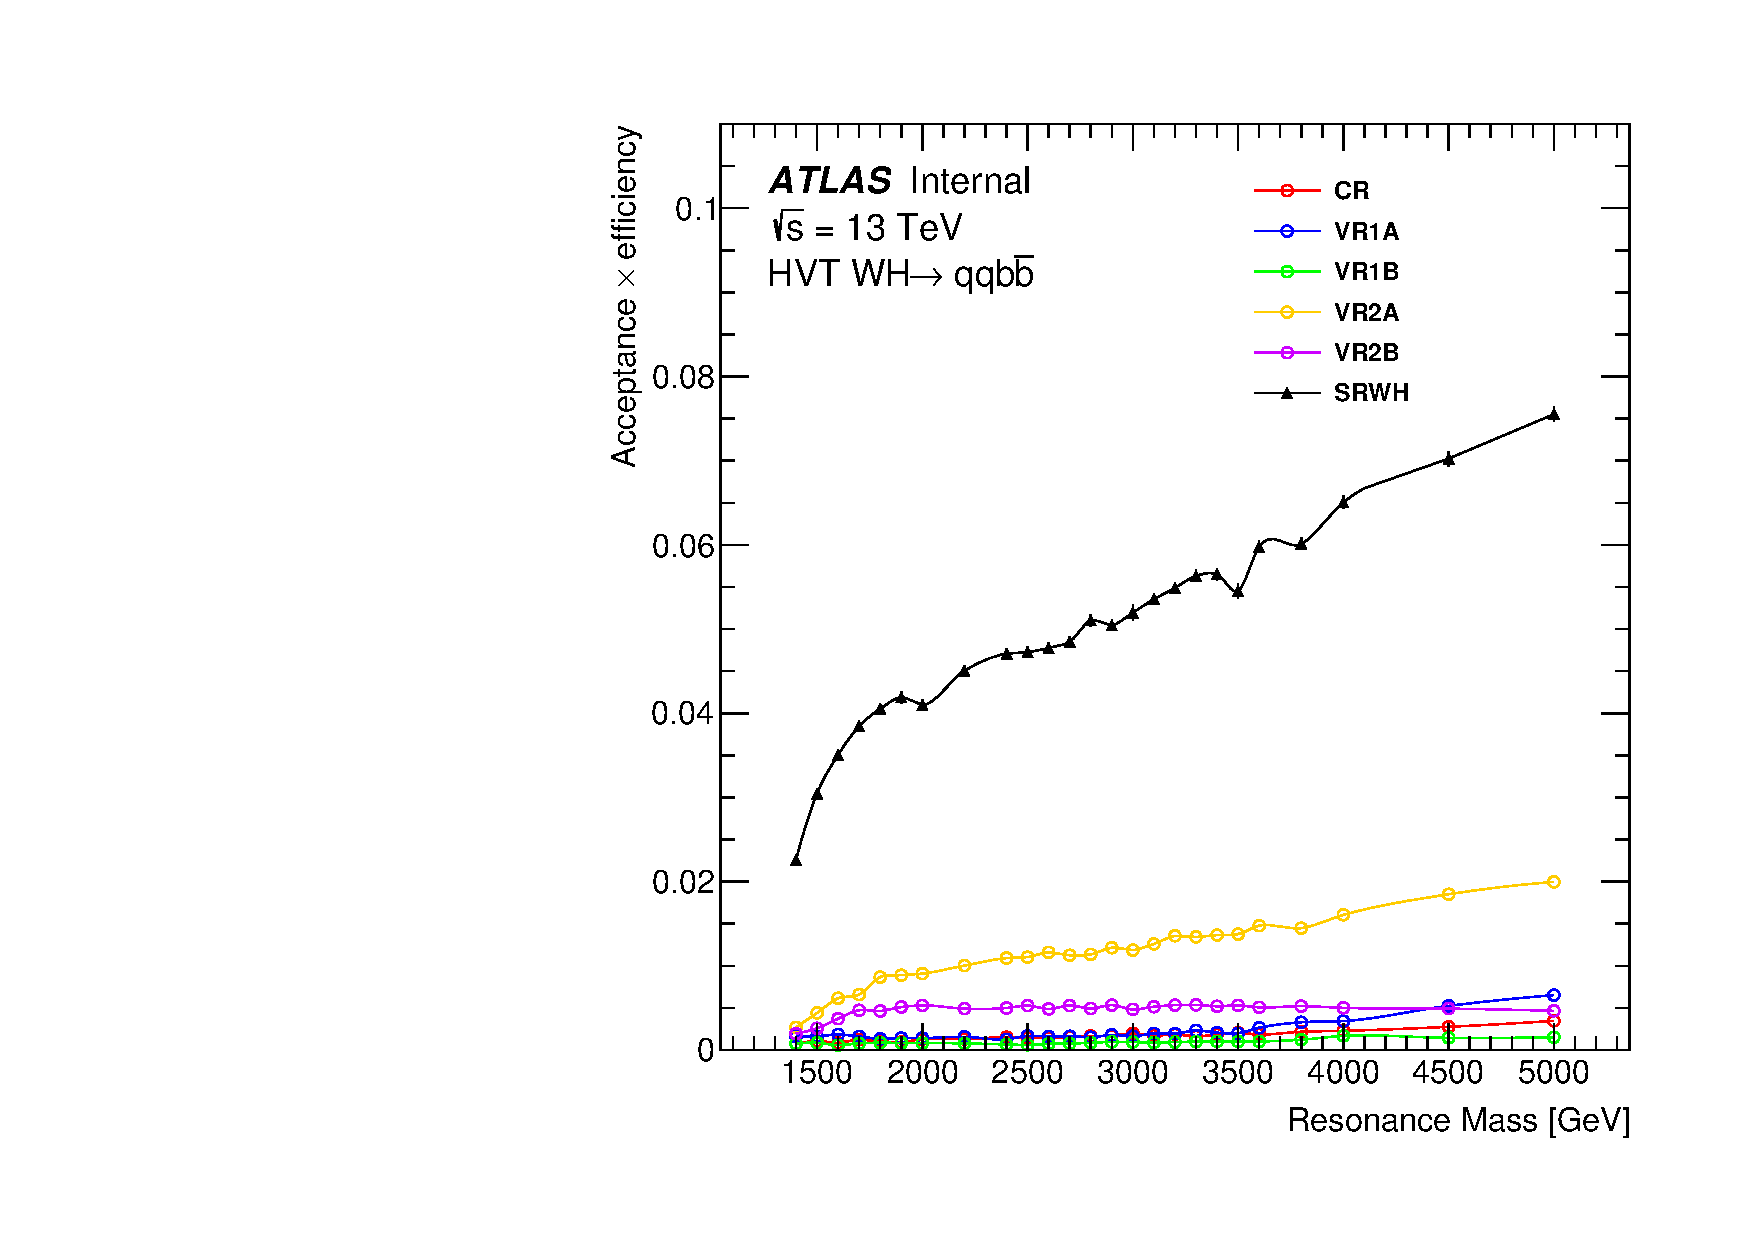
\includegraphics[width=0.49\textwidth]{VHqqbb_Region_Efficiency_Comparison_WH_Ntag1.pdf}
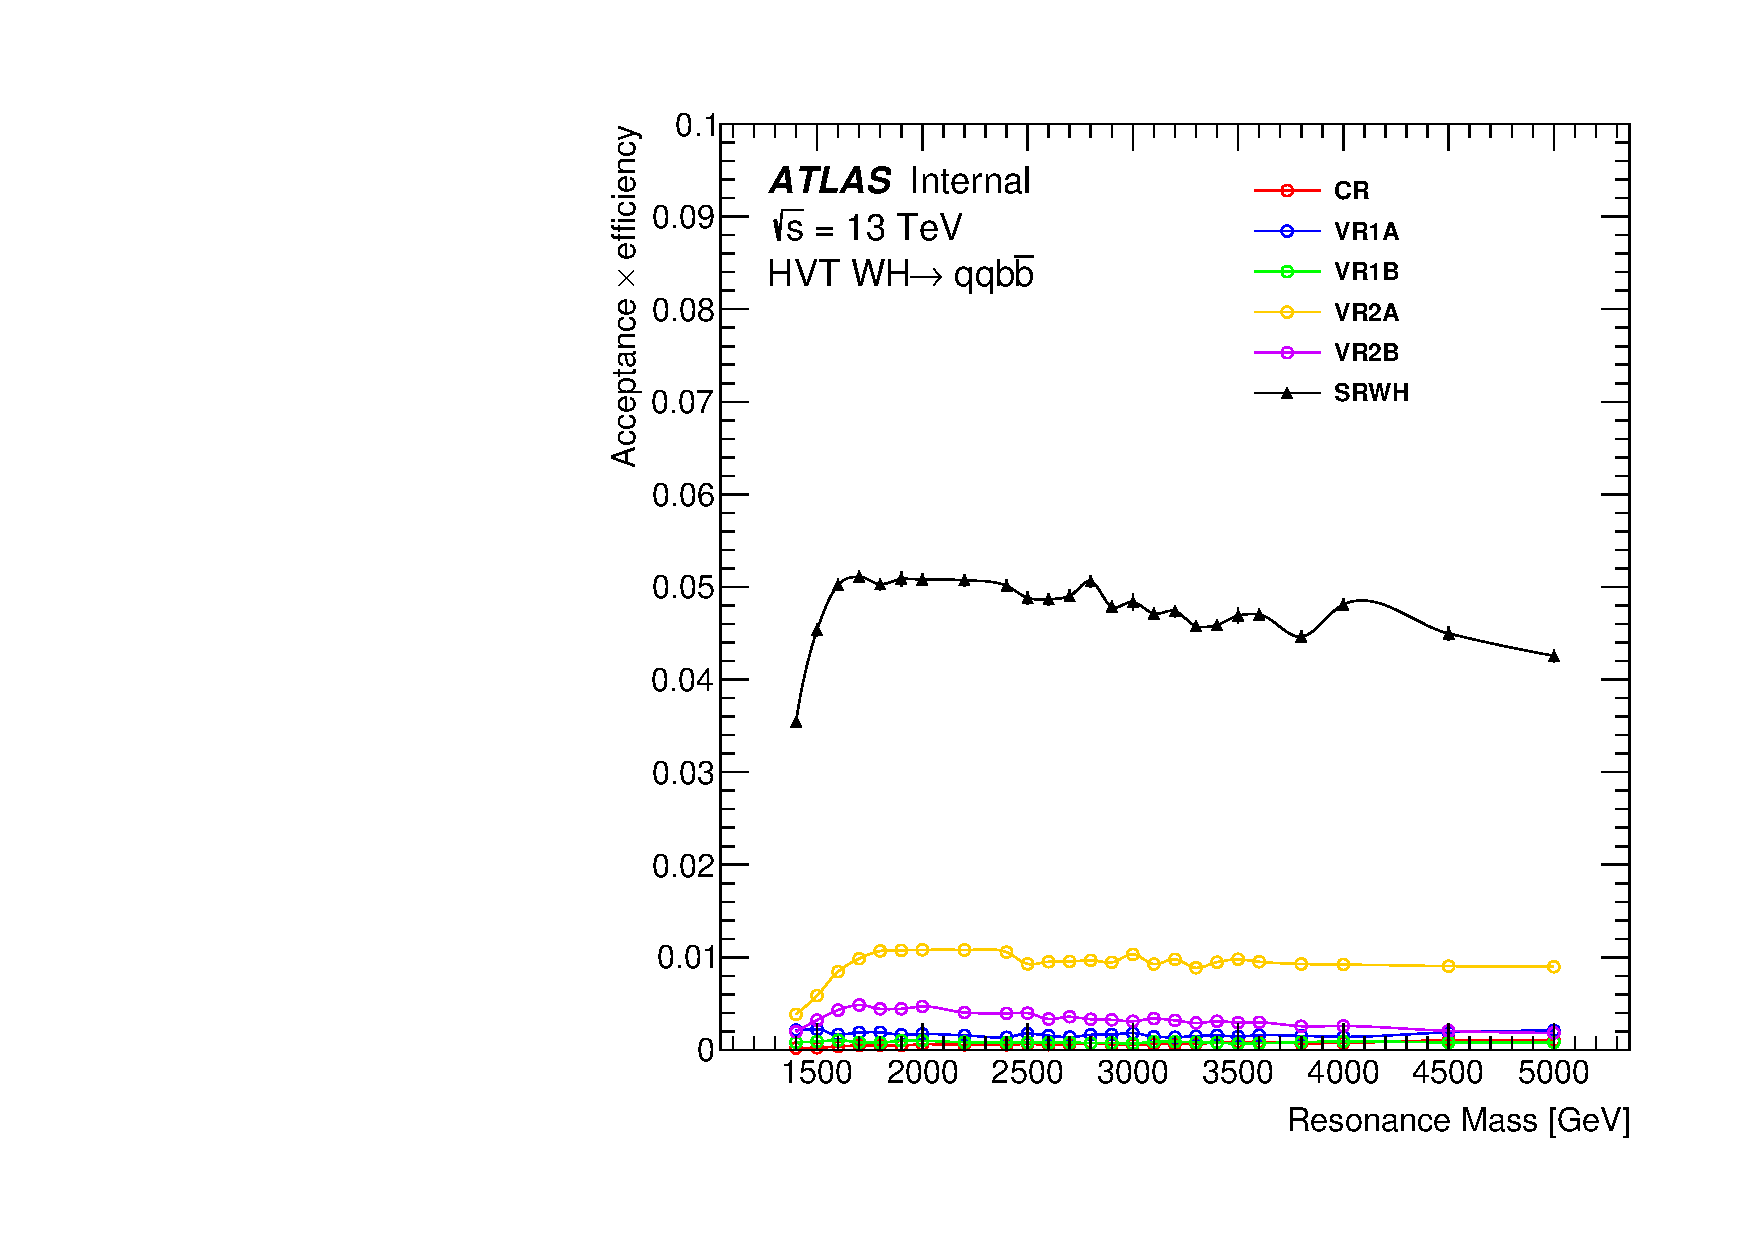
\includegraphics[width=0.49\textwidth]{VHqqbb_Region_Efficiency_Comparison_WH_Ntag2.pdf} \\
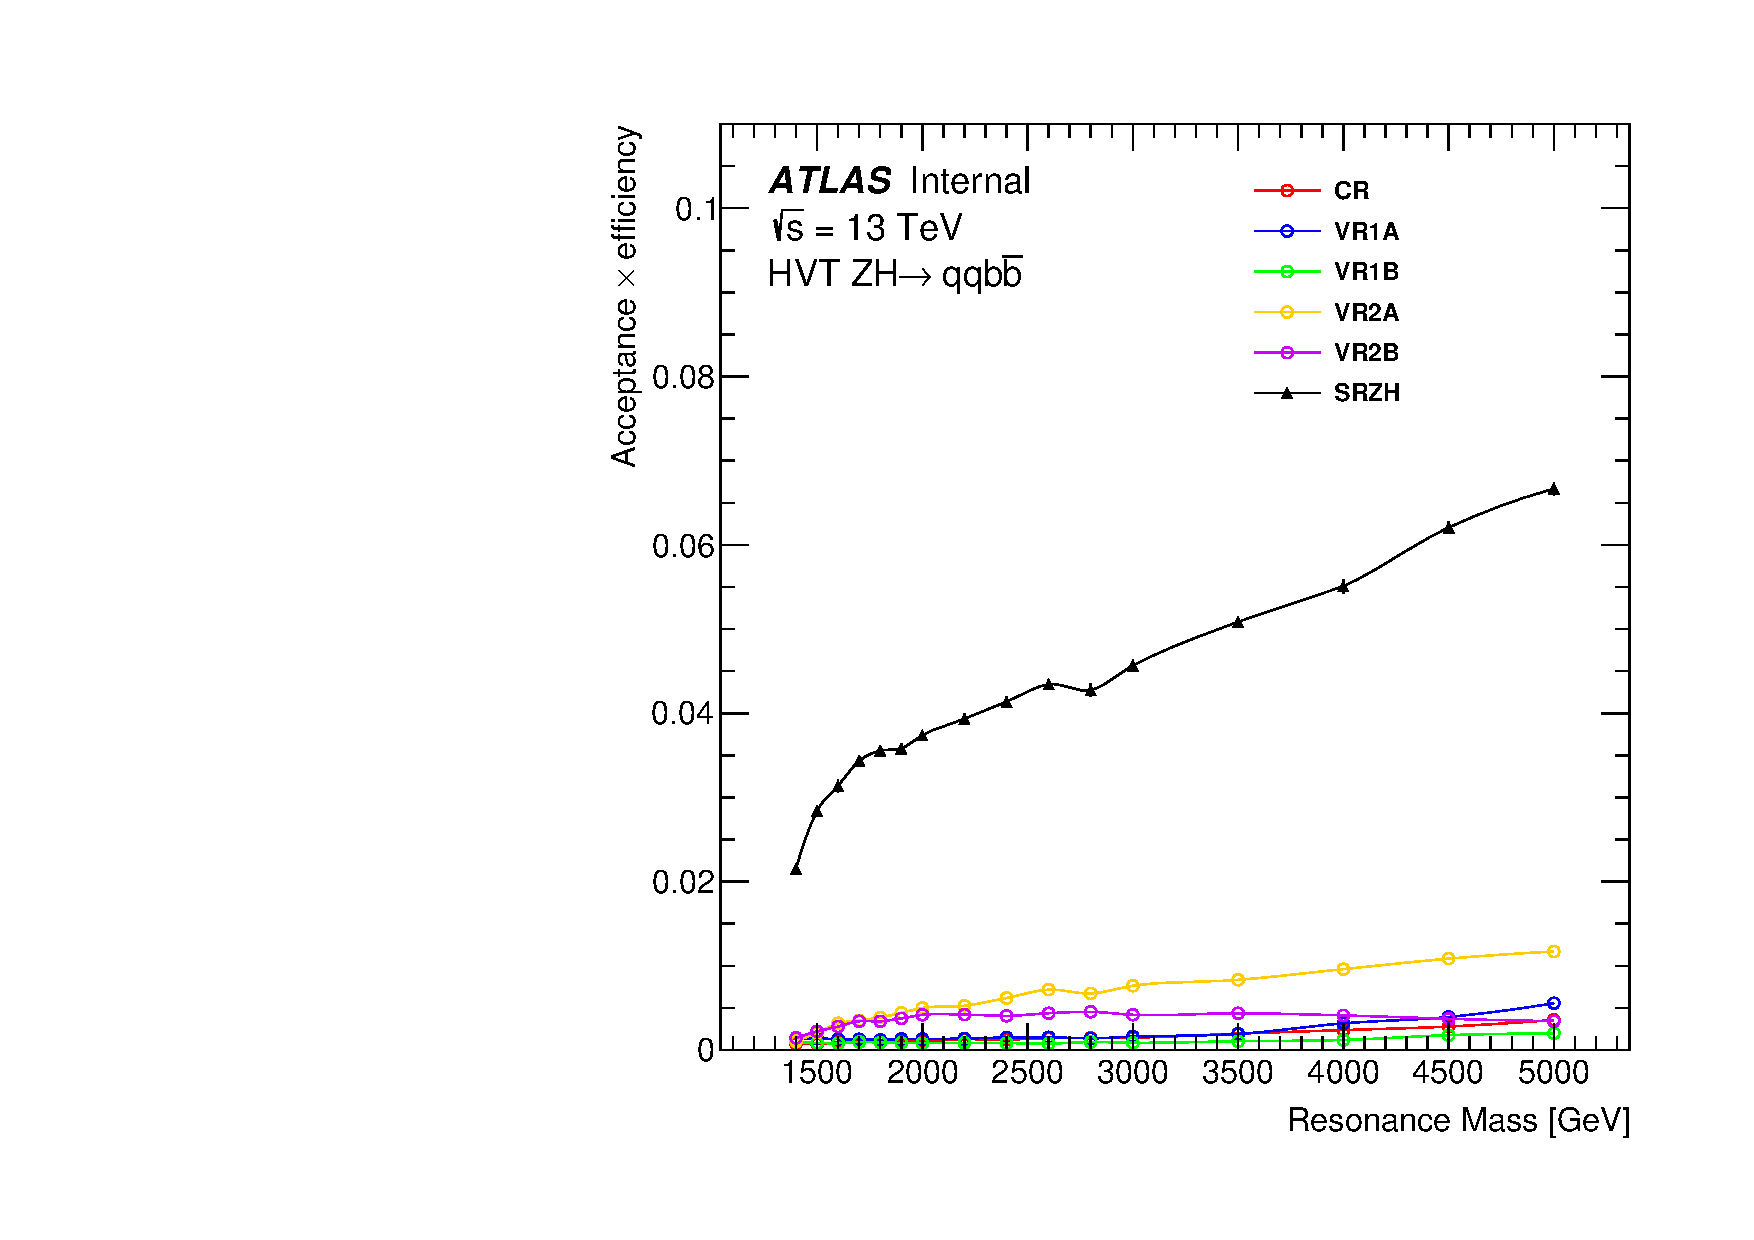
\includegraphics[width=0.49\textwidth]{VHqqbb_Region_Efficiency_Comparison_ZH_Ntag1.pdf}
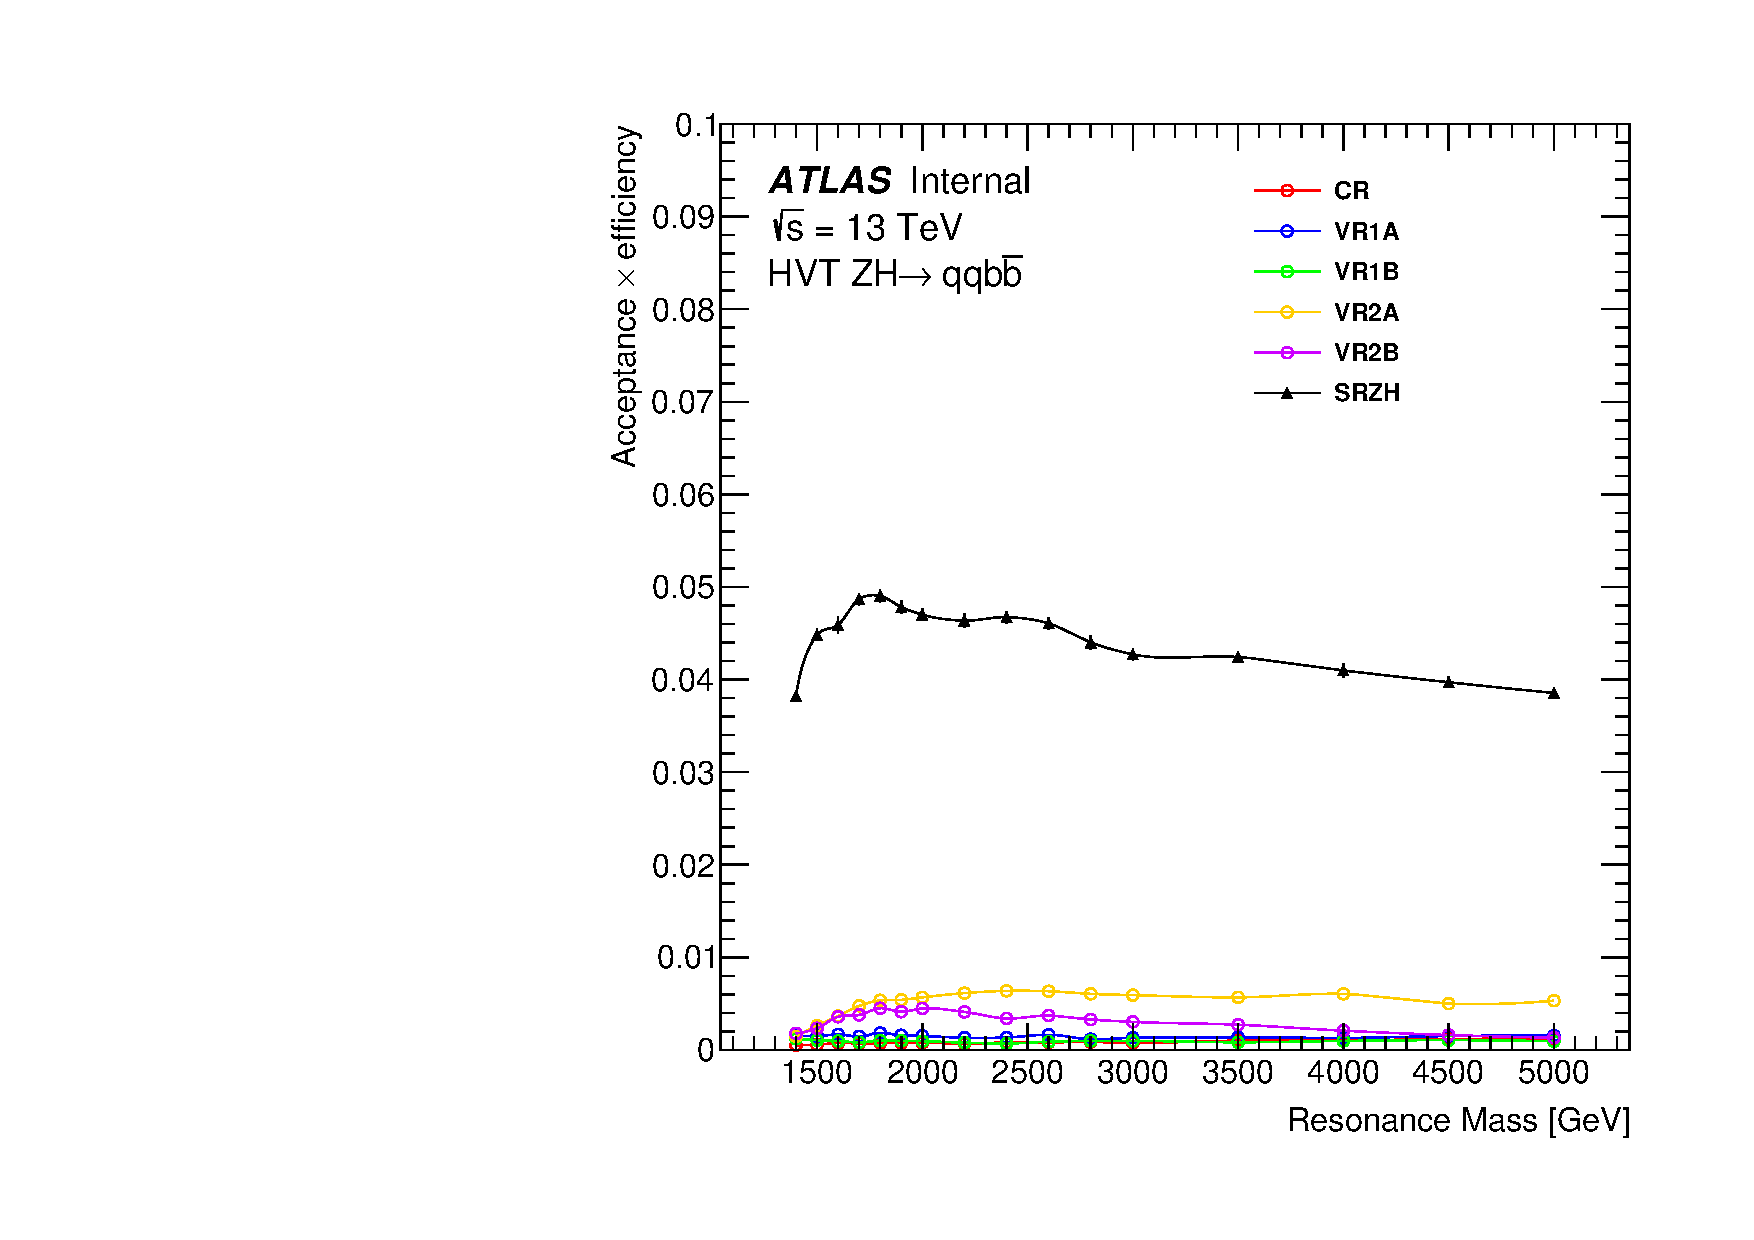
\includegraphics[width=0.49\textwidth]{VHqqbb_Region_Efficiency_Comparison_ZH_Ntag2.pdf}
\end{center}
\caption{
    Comparison of signal efficiency for the various control, validation, and signal regions. The WH (top row) and ZH (bottom row) samples are shown for each channel: 1-tag (left column) and 2-tag (right column).
    The black line shows the corresponding signal region and the colored lines show the control and validation regions.
}
\label{fig:sig_contam}
\end{figure}

Defining the various regions this way is motivated by the relative independence of b-tagging efficiency and large-R jet mass for QCD jets, as demonstrated in Figure~\ref{fig:bkg_btag_eff}.
This independence helps in large part to satisfy the requirement that the re-weighting procedure derived in the control region is applicable to the signal and validation regions.
Signal contamination levels in the control and validation regions are small enough to be ignored in all cases, as shown in Figure ~\ref{fig:sig_contam}. 

\begin{figure}[htbp!]
\begin{center}
    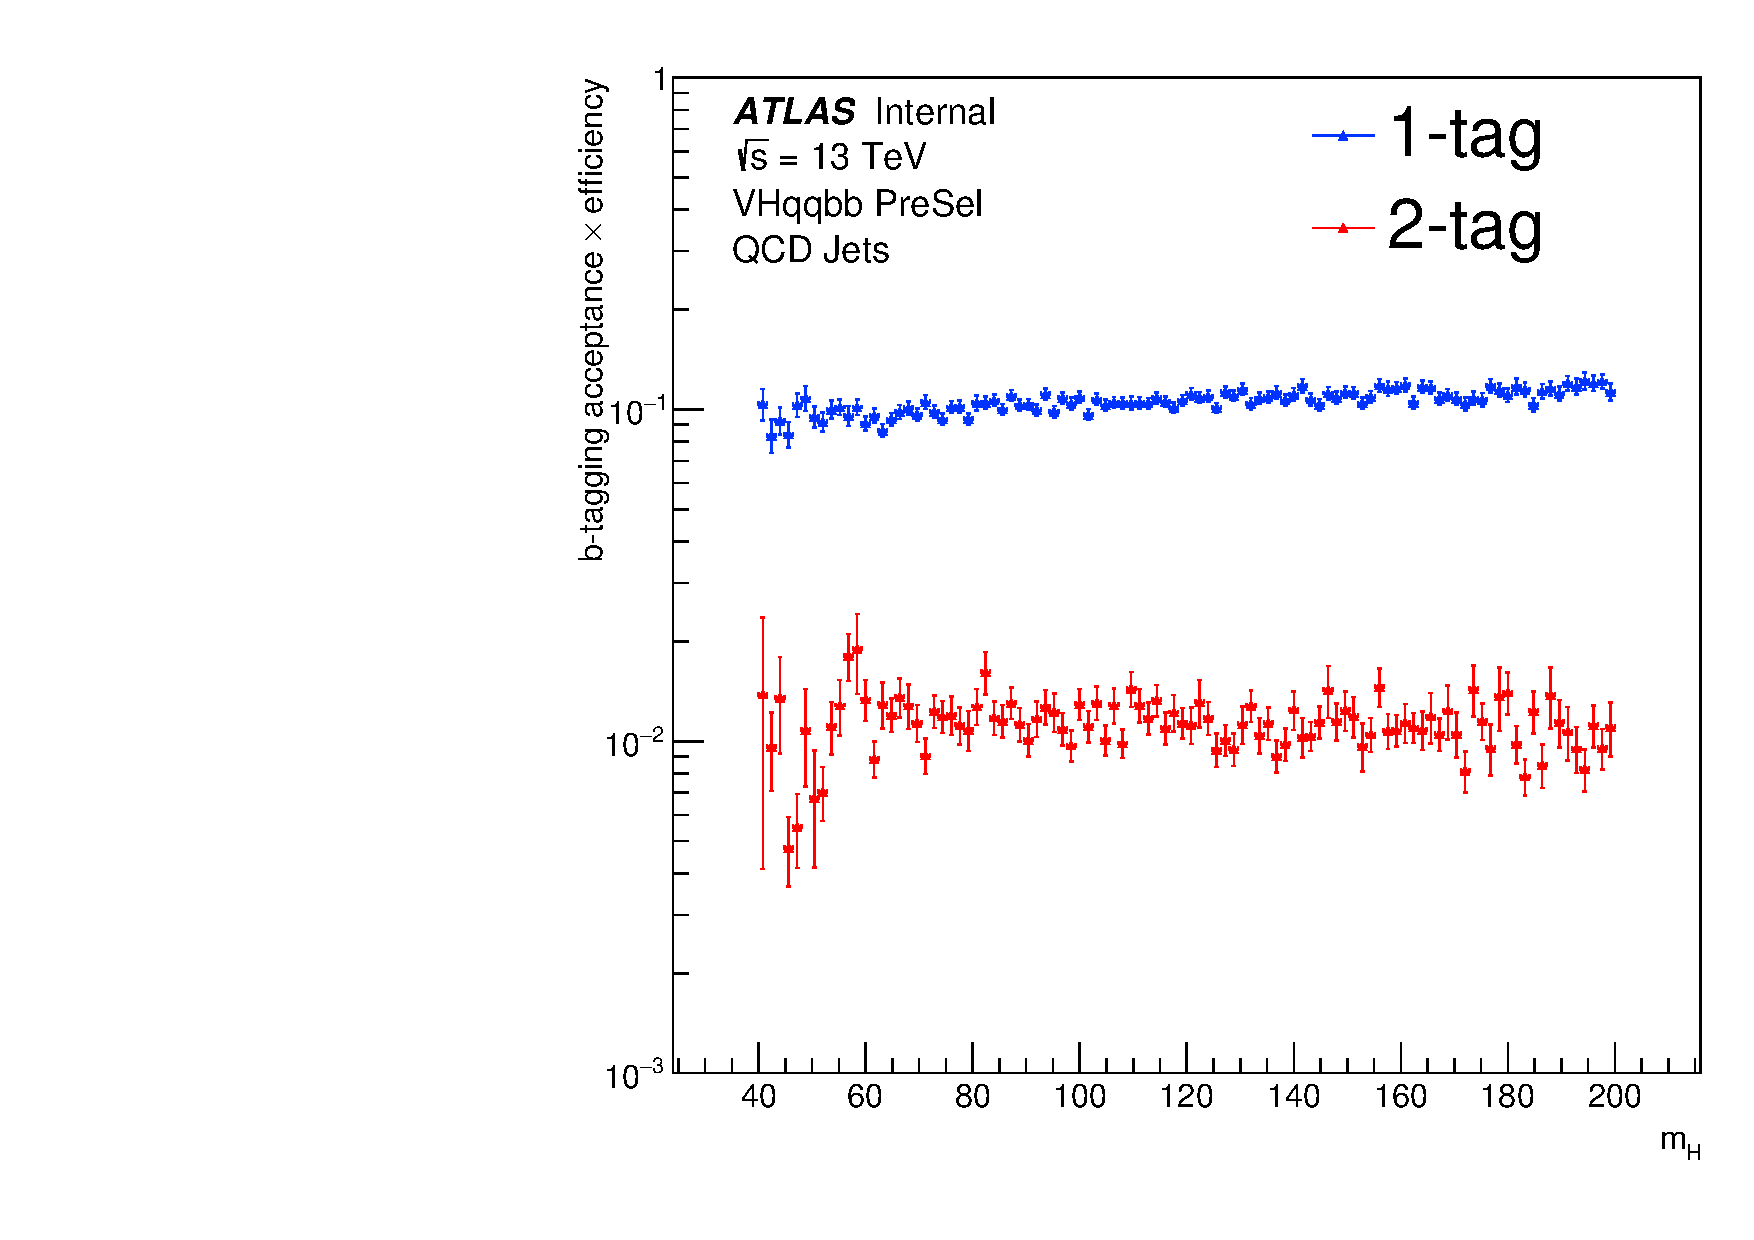
\includegraphics[width=0.49\textwidth]{PlotBtagRej_mH.pdf}
\end{center}
\caption{The efficiency of 1/2-tag categorization for QCD MC events as a function of the Higgs candidate Large-R jet mass, starting from the loose pre-selection as described in Section~\ref{subsec:presel}, both for 1-tag and 2-tag. }
\label{fig:bkg_btag_eff}
\end{figure}

In order to preserve similarity to the signal regions, the Higgs \ntrk cut is applied to all control and validation regions as well.
The $D_2$ cut is not applied to the $W/Z$ candidate for the control or validation regions, as it has only a very small correlation with $m_{JJ}$ and reduces the statistics available for re-weighting training/validation.
A detailed description of all regions is given in Table~\ref{tab:RegionDefinition}.
The estimated relative contribution of each background from MC is given in Table~\ref{tab:bkg_comp}.
The yields for all signal, control and validations regions for the full Run 2 data set are shown in Table \ref{tab:cr_vr_yield}.

\begin{table}[htbp!]
\begin{tiny}
\begin{center}
\begin{tabular}{c|c|c|c}
    Region & Boson Tagger Pass/Fail & Additional Cuts & Comments \\
\hline
\hline
    \makecell{WH Signal Region \\ (SRWH)} & \makecell{$W \land H$} & \makecell{N/A} & \makecell{Used in the final likelihood fit} \\
\hline
    \makecell{ZH Signal Region \\ (SRZH)} & \makecell{$Z \land H$} & \makecell{N/A} & \makecell{Used in the final likelihood fit} \\
\hline
    \makecell{Control Region \\ (CR)} & \makecell{Fail SRWH/SRZH Cuts \\ Pass H \ntrk Cut} & \makecell{$(m_V < 65\ GeV \land m_H < 70\ GeV)\ \lor$ \\ $(m_V > 110\ GeV \land m_H > 150\ GeV)\ \lor$ \\ $(m_V < 65\ GeV \land m_H > 150\ GeV)$ \\ See Figure~\ref{fig:crvr_plane}.} & \makecell{Used to train BDT in the kinematic reweighting} \\
\hline
    \makecell{Validation Region \\ (VR1A)} & \makecell{Fail SRWH/SRZH Cuts \\ Pass H \ntrk Cut \\ Pass W or Z \ntrk cut} & \makecell{$m_H > 150\ GeV$ \\ $m_V > 65\ GeV$ \\ $m_V < 110\ GeV$} & \makecell{Used to validate background estimation \\ and derive associated modeling uncertainties} \\
\hline
    \makecell{Validation Region \\ (VR1B)} & \makecell{Fail SRWH/SRZH Cuts \\ Pass H \ntrk Cut \\ Fail W and Z \ntrk cuts} & \makecell{$m_H > 150\ GeV$ \\ $m_V > 65\ GeV$ \\ $m_V < 110\ GeV$} & \makecell{Used to validate background estimation \\ and derive associated modeling uncertainties} \\
\hline
    \makecell{Validation Region \\ (VR2A)} & \makecell{Fail SRWH/SRZH Cuts \\ Pass H \ntrk Cut \\ Pass W or Z \ntrk cut} & \makecell{$m_H > 70\ GeV$ \\ $m_H < 150\ GeV$ \\ $m_V < 65\ GeV$} & \makecell{Used to validate background estimation \\ and derive associated modeling uncertainties} \\
\hline
    \makecell{Validation Region \\ (VR2B)} & \makecell{Fail SRWH/SRZH Cuts \\ Pass H \ntrk Cut \\ Fail W and Z \ntrk cuts} & \makecell{$m_H > 70\ GeV$ \\ $m_H < 150\ GeV$ \\ $m_V < 65\ GeV$} & \makecell{Used to validate background estimation \\ and derive associated modeling uncertainties} \\
\hline
\end{tabular}
\end{center}
\end{tiny}
\caption{Definition of all signal, control, and validation regions.}
\label{tab:RegionDefinition}
\end{table}

\begin{figure}[htbp!]
\begin{center}
    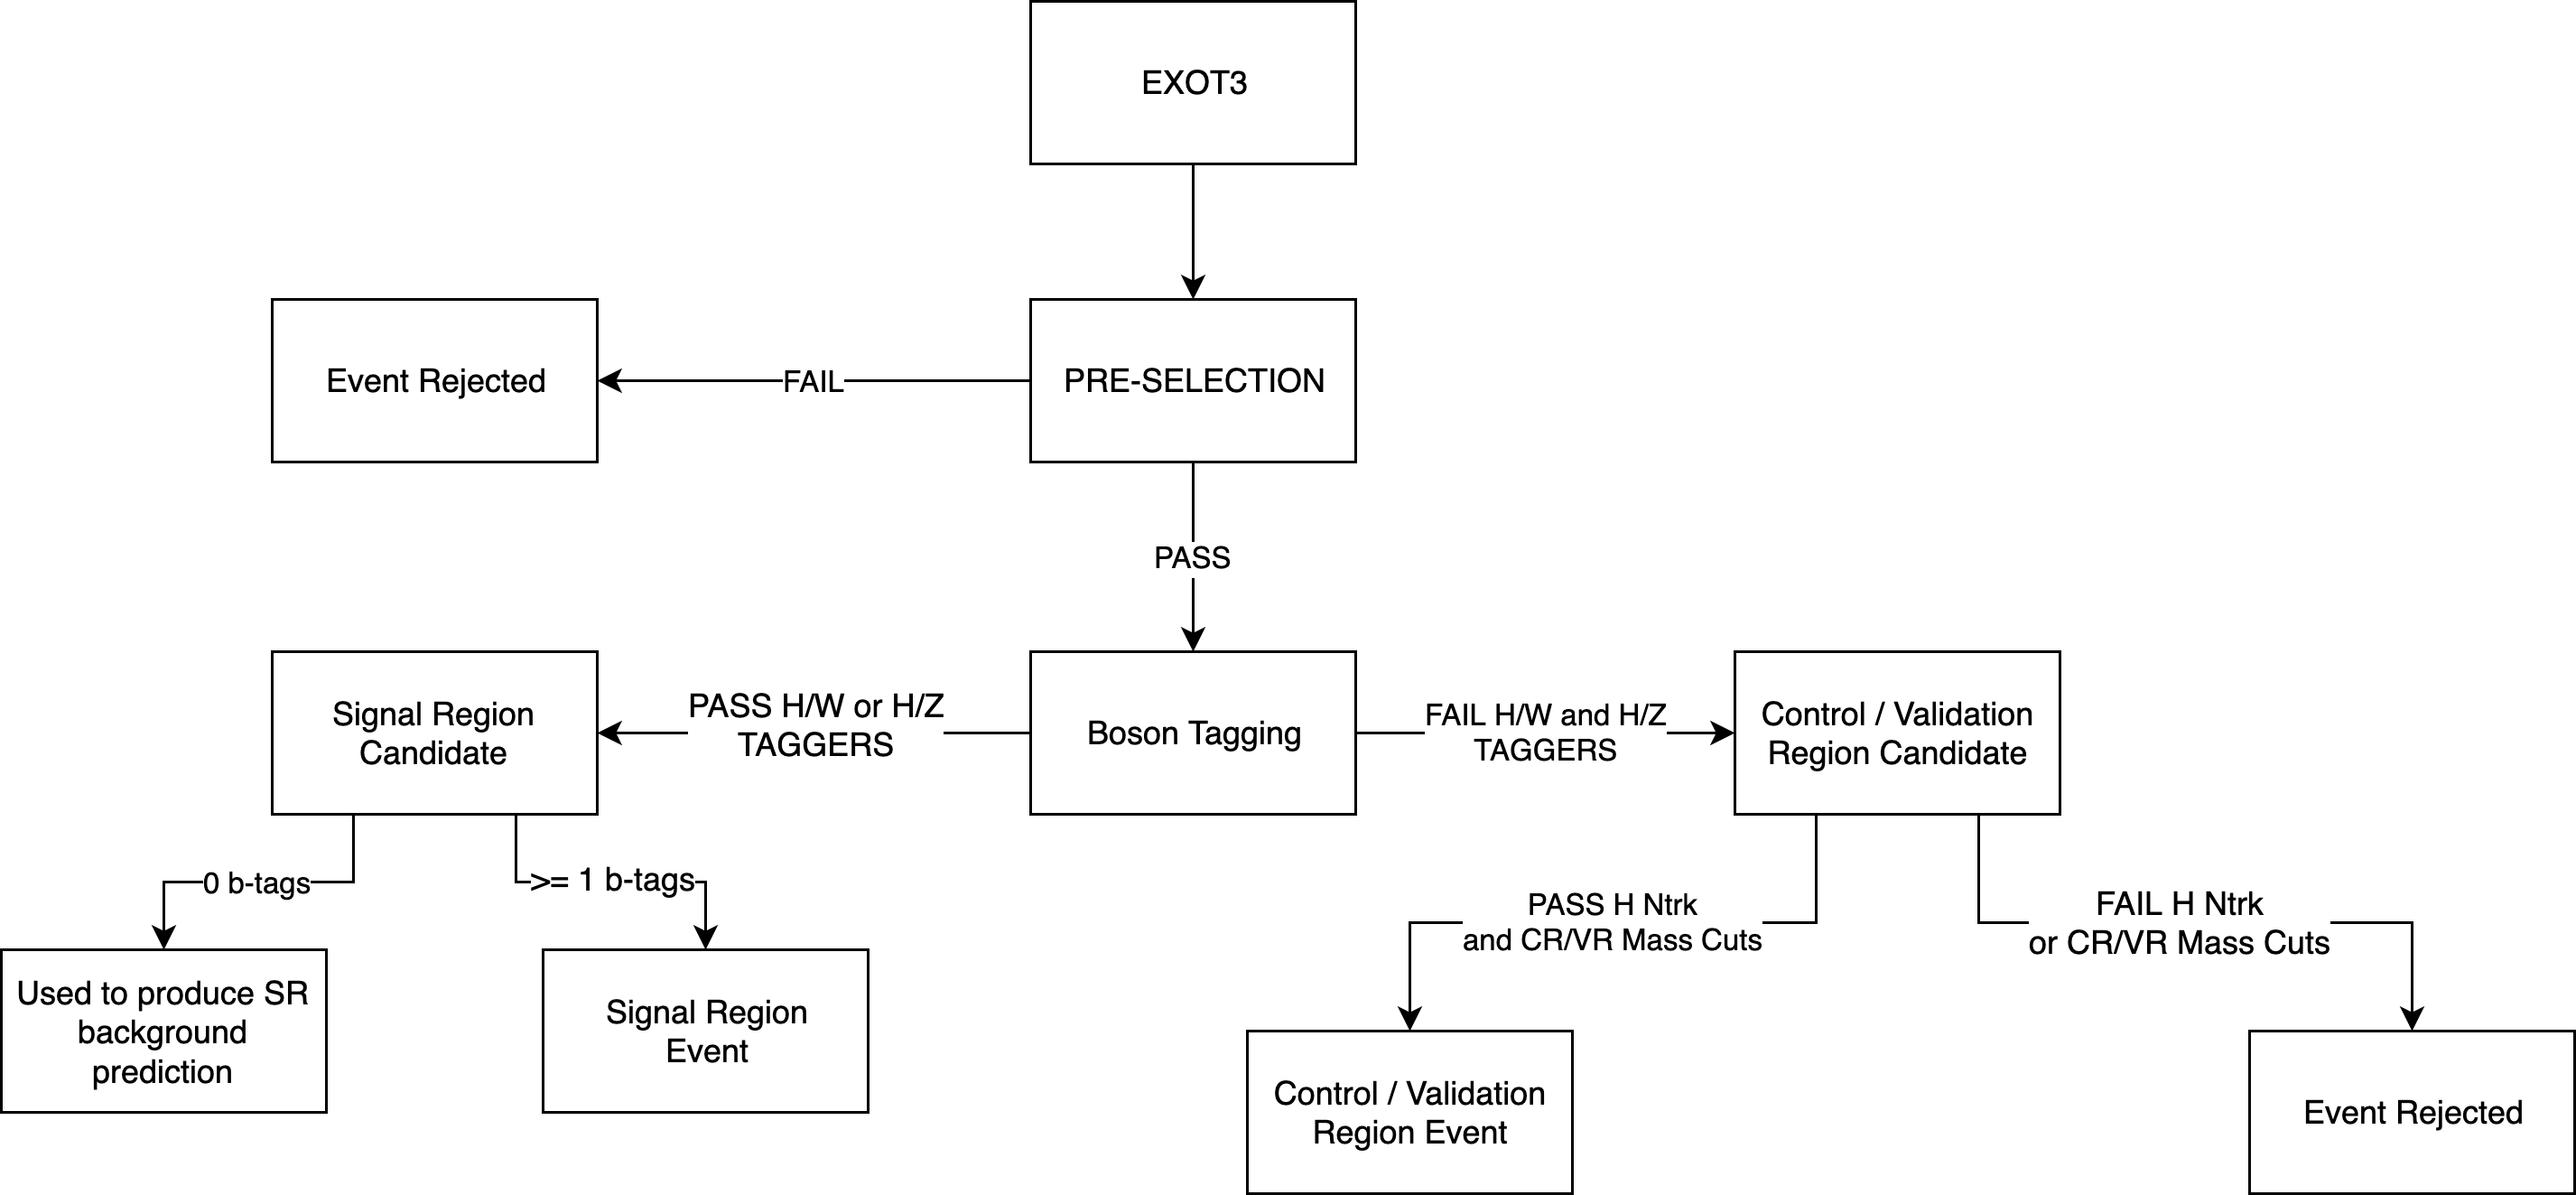
\includegraphics[width=\textwidth]{VHqqbb_Selection_Flowchart}
\end{center}
\caption{ Flowchart outlining the signal, control, and validation region selection. }
\label{fig:selection_flowchart}
\end{figure}

\begin{table}[!htb]
%\begin{scriptsize}
\begin{center}
\begin{tabular}{|c|c|c|c|}
\hline
Region/Channel & QCD Yield [\%] & $t\bar{t}$ Yield [\%] & V+Jets Yield [\%]  \\ \hline
CR 0-tag & 98.69 $\pm$ 0.55 & 0.73 $\pm$ 0.01 & 0.58 $\pm$ 0.03 \\
\hline
CR 1-tag & 94.39 $\pm$ 1.23 & 5.13 $\pm$ 0.07 & 0.48 $\pm$ 0.07 \\
\hline
CR 2-tag & 94.48 $\pm$ 3.77 & 5.18 $\pm$ 0.23 & 0.34 $\pm$ 0.21 \\
\hline
VR1A 0-tag & 96.58 $\pm$ 2.36 & 0.8 $\pm$ 0.05 & 2.62 $\pm$ 0.23 \\
\hline
VR1A 1-tag & 92.49 $\pm$ 5.06 & 5.49 $\pm$ 0.32 & 2.02 $\pm$ 0.45 \\
\hline
VR1A 2-tag & 95.25 $\pm$ 14.05 & 3.11 $\pm$ 0.68 & 1.64 $\pm$ 0.98 \\
\hline
VR2A 0-tag & 98.38 $\pm$ 1.16 & 0.04 $\pm$ 0.01 & 1.58 $\pm$ 0.10 \\
\hline
VR2A 1-tag & 98.06 $\pm$ 2.81 & 0.31 $\pm$ 0.04 & 1.63 $\pm$ 0.22 \\
\hline
VR2A 2-tag & 97.23 $\pm$ 7.4 & 0.36 $\pm$ 0.11 & 2.41 $\pm$ 0.90 \\
\hline
VR1B 0-tag & 98.49 $\pm$ 0.91 & 0.5 $\pm$ 0.01 & 1.01 $\pm$ 0.06 \\
\hline
VR1B 1-tag & 95.97 $\pm$ 1.92 & 3.35 $\pm$ 0.09 & 0.69 $\pm$ 0.11 \\
\hline
VR1B 2-tag & 95.69 $\pm$ 6.0 & 3.44 $\pm$ 0.29 & 0.87 $\pm$ 0.69 \\
\hline
VR2B 0-tag & 98.37 $\pm$ 0.6 & 0.06 $\pm$ 0.01 & 1.57 $\pm$ 0.05 \\
\hline
VR2B 1-tag & 97.37 $\pm$ 1.44 & 0.38 $\pm$ 0.02 & 2.25 $\pm$ 0.14 \\
\hline
VR2B 2-tag & 97.21 $\pm$ 4.13 & 0.17 $\pm$ 0.06 & 2.62 $\pm$ 0.37 \\
\hline
\end{tabular}
\caption{Breakdown of Monte Carlo background composition in each region/channel.
         The signal regions are not included due to lack of Monte Carlo statistics preventing a meaningful estimate.
         The errors displayed are purely statistical.
     }
\label{tab:bkg_comp}
\end{center}
%\end{scriptsize}
\end{table}

\begin{table}[!htb]
%\begin{scriptsize}
\begin{center}
\begin{tabular}{|c|c|c|c|}
\hline
Region & 0-tag Events (\lumi) & 1-tag Events (\lumi) & 2-tag Events (\lumi) \\ \hline
CR & 300635 & 48112 & 4918 \\
\hline
VR1A & 26376 & 4359 & 495 \\
\hline
VR1B & 111420 & 18198 & 1895 \\
\hline
VR2A & 77092 & 11635 & 1311 \\
\hline
VR2B & 192257 & 29064 & 3015 \\
\hline
SRWH & 4362 & 598 & 57 \\
\hline
SRZH & 5038 & 717 & 84 \\
\hline
\end{tabular}
\caption{Yields in the full Run 2 data set for each signal, control and validation region.}
\label{tab:cr_vr_yield}
\end{center}
%\end{scriptsize}
\end{table}

\subsection{Normalization}
\label{sec:bkg-normalization}
As mentioned previously, three channels are distinguished for all regions: 0-tag, 1-tag, and 2-tag.
These channels are defined by the b-tagging pass/fail status for each of the two leading \pt\ ghost-associated track jets of the Higgs candidate large-R jet.
Events from the 0-tag channel are used to estimate the shape of the background in the corresponding 1-tag and 2-tag channels.
For all regions the 0-tag channel is $> 98\%$ pure in QCD events, as predicted by MC.

It should be noted that the 0-tag sample has one additional requirement that the Higgs candidate must have at least as many ghost-associated track jets as the number of b-tags in the channel being modeled.
So when modeling the 1(2)-tag sample, the 0-tag Higgs candidate must have at least 1 (2) matched track jet(s).
This requirement helps to ensure that the kinematics of the 0-tag sample is as close as possible to the tagged SR being modeled.

Separately from the kinematic shape re-weighting, a normalization factor for estimating the yield ratio of the 1/2-tag channel to the 0-tag channel must be derived.
We label these scale factors as $\mu_{0 \rightarrow 1}$ and $\mu_{0 \rightarrow 2}$.
These scale factors are not identical in all regions, as show in Fig ~\ref{fig:CompareMu}.  % Due primarily to small differences in QCD flavor composition as well as $t\bar{t}$ and $V$+jets contribution?
The goal is then to develop a strategy for predicting $\mu_{0 \rightarrow 1}$ and $\mu_{0 \rightarrow 2}$ in the signal regions, along with a corresponding statistical and systematic error.

As mentioned previously, modelling the background shape with MC is not a reliable strategy for this analysis.
For this reason the data from the control and validation regions are used to estimate the nominal values and uncertainties of \muOne and \muTwo.
The nominal values are taken from the control region (CR).
A systematic error for each channel is defined conservatively by the largest $\mu$ difference between any two regions.
The nominal values and errors for both normalization scale factors are:
\begin{align}
    \mu_{0 \rightarrow 1} &= 0.160 \pm 0.014\ \mathrm{(syst.)} \pm 7 \times 10^{-4}\ \mathrm{(stat.)} \\
    \mu_{0 \rightarrow 2} &= 0.0167 \pm 0.0028\ \mathrm{(syst.)} \pm 2 \times 10^{-4}\ \mathrm{(stat.)}
\end{align}

\begin{figure}[htbp!]
\begin{center}
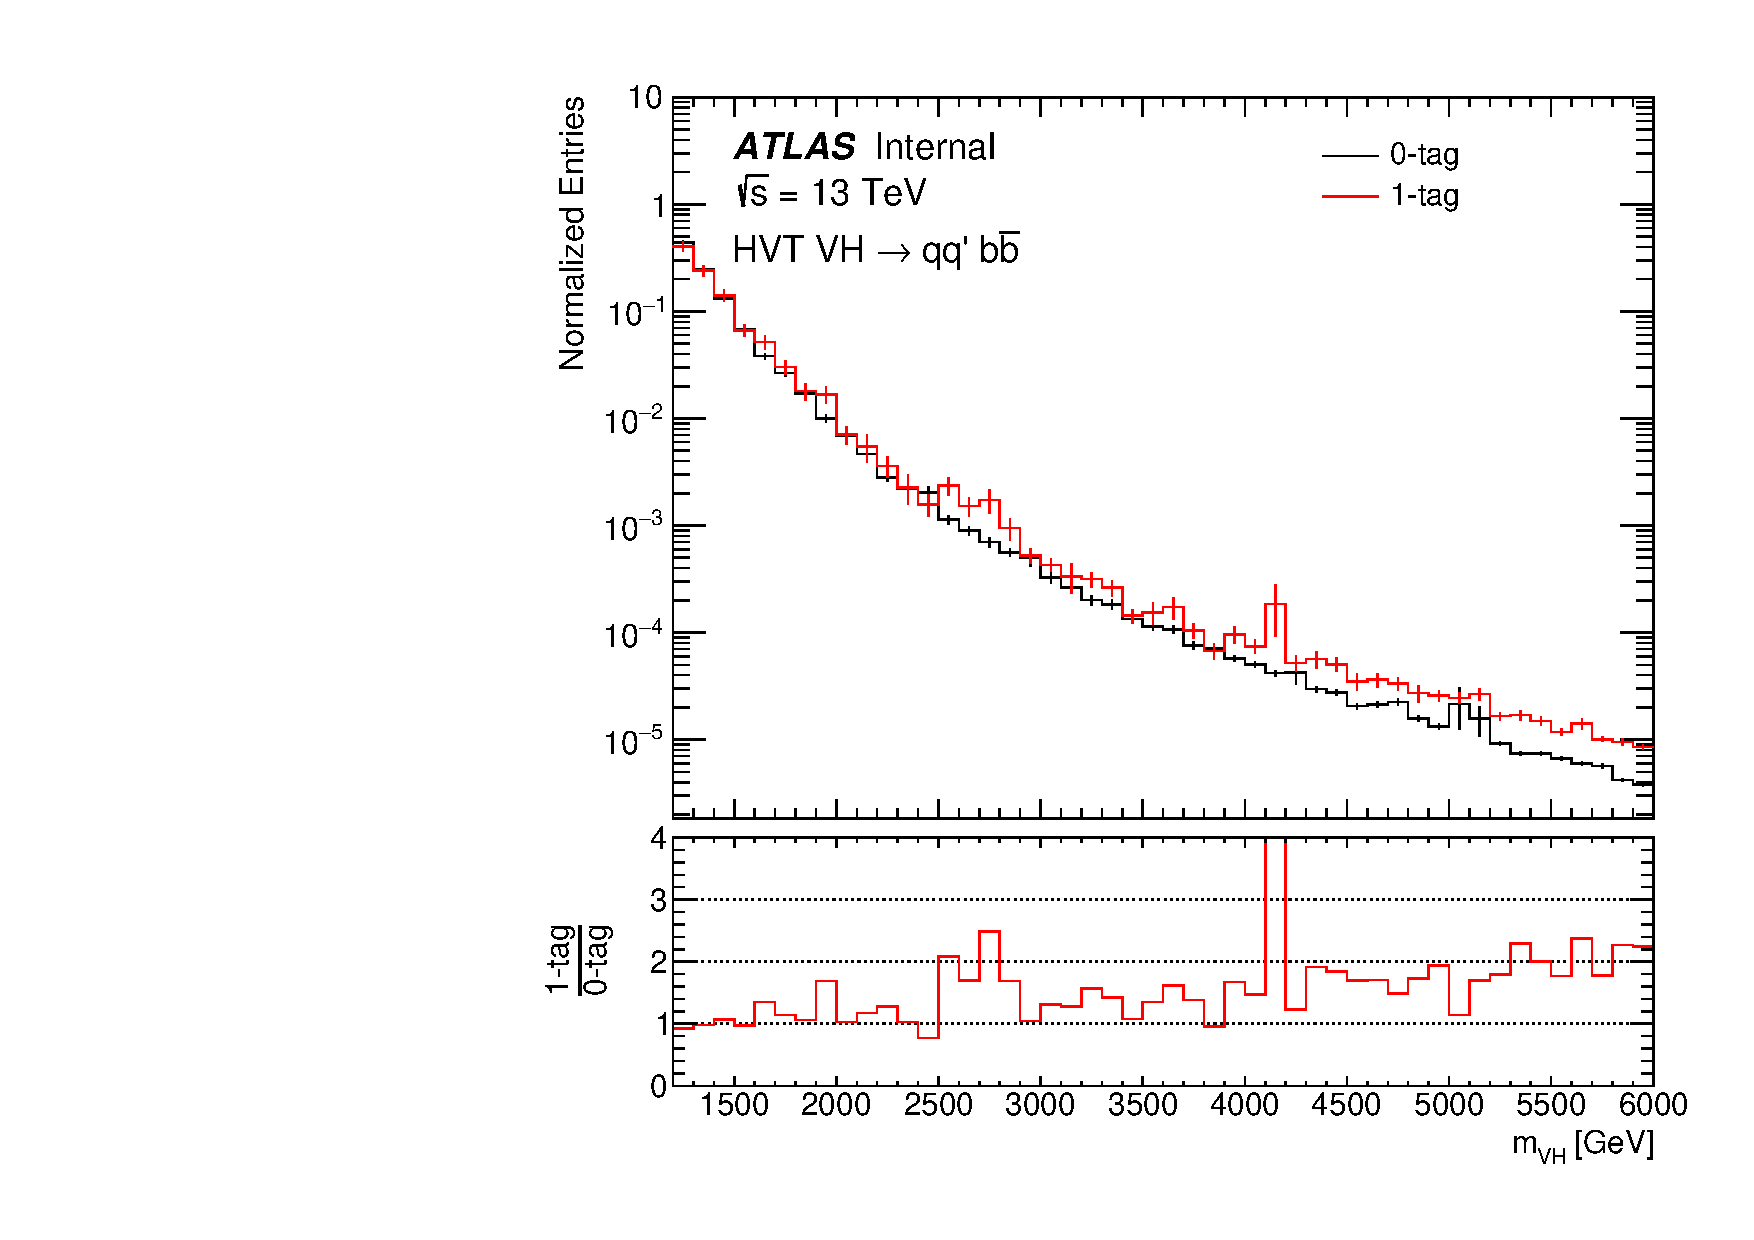
\includegraphics[width=0.49\textwidth]{VHqqbb_mVH_BTagRatio_0_to_1_MC.pdf}
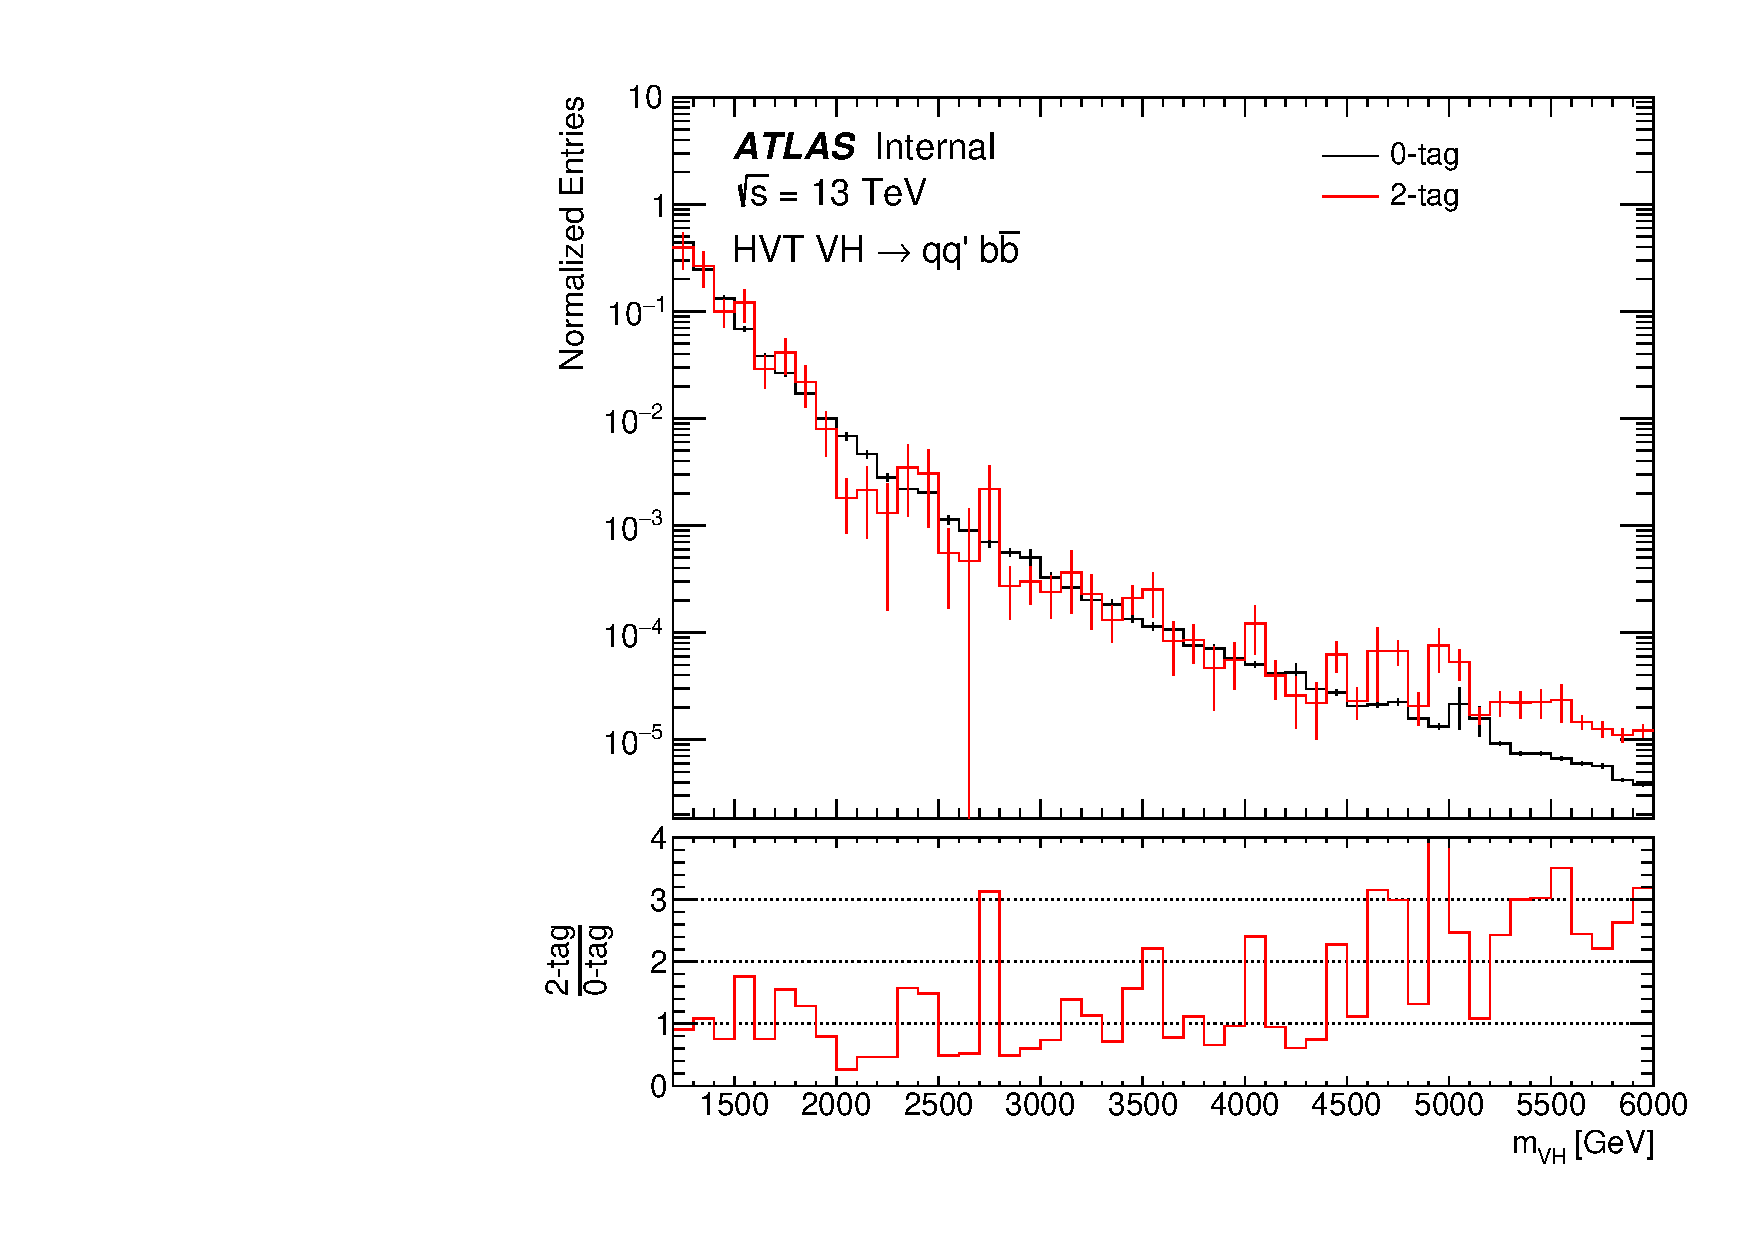
\includegraphics[width=0.49\textwidth]{VHqqbb_mVH_BTagRatio_0_to_2_MC.pdf}
\end{center}
\caption{Comparison of 0-tag SR background shape to the 1-tag (left) and 2-tag (right) SR background shapes in simulated multijet data.
The SRWH and SRZH signal regions are combined and distributions are normalized to unity.
The trends obvious in the ratio plots demonstrate the need for kinematic re-weighting when utilizing the 0-tag data to produce background estimates for 1-tag and 2-tag channels.
}
\label{fig:bkg_0tag_comp}
\end{figure}

\begin{figure}[htbp!]
\begin{center}
    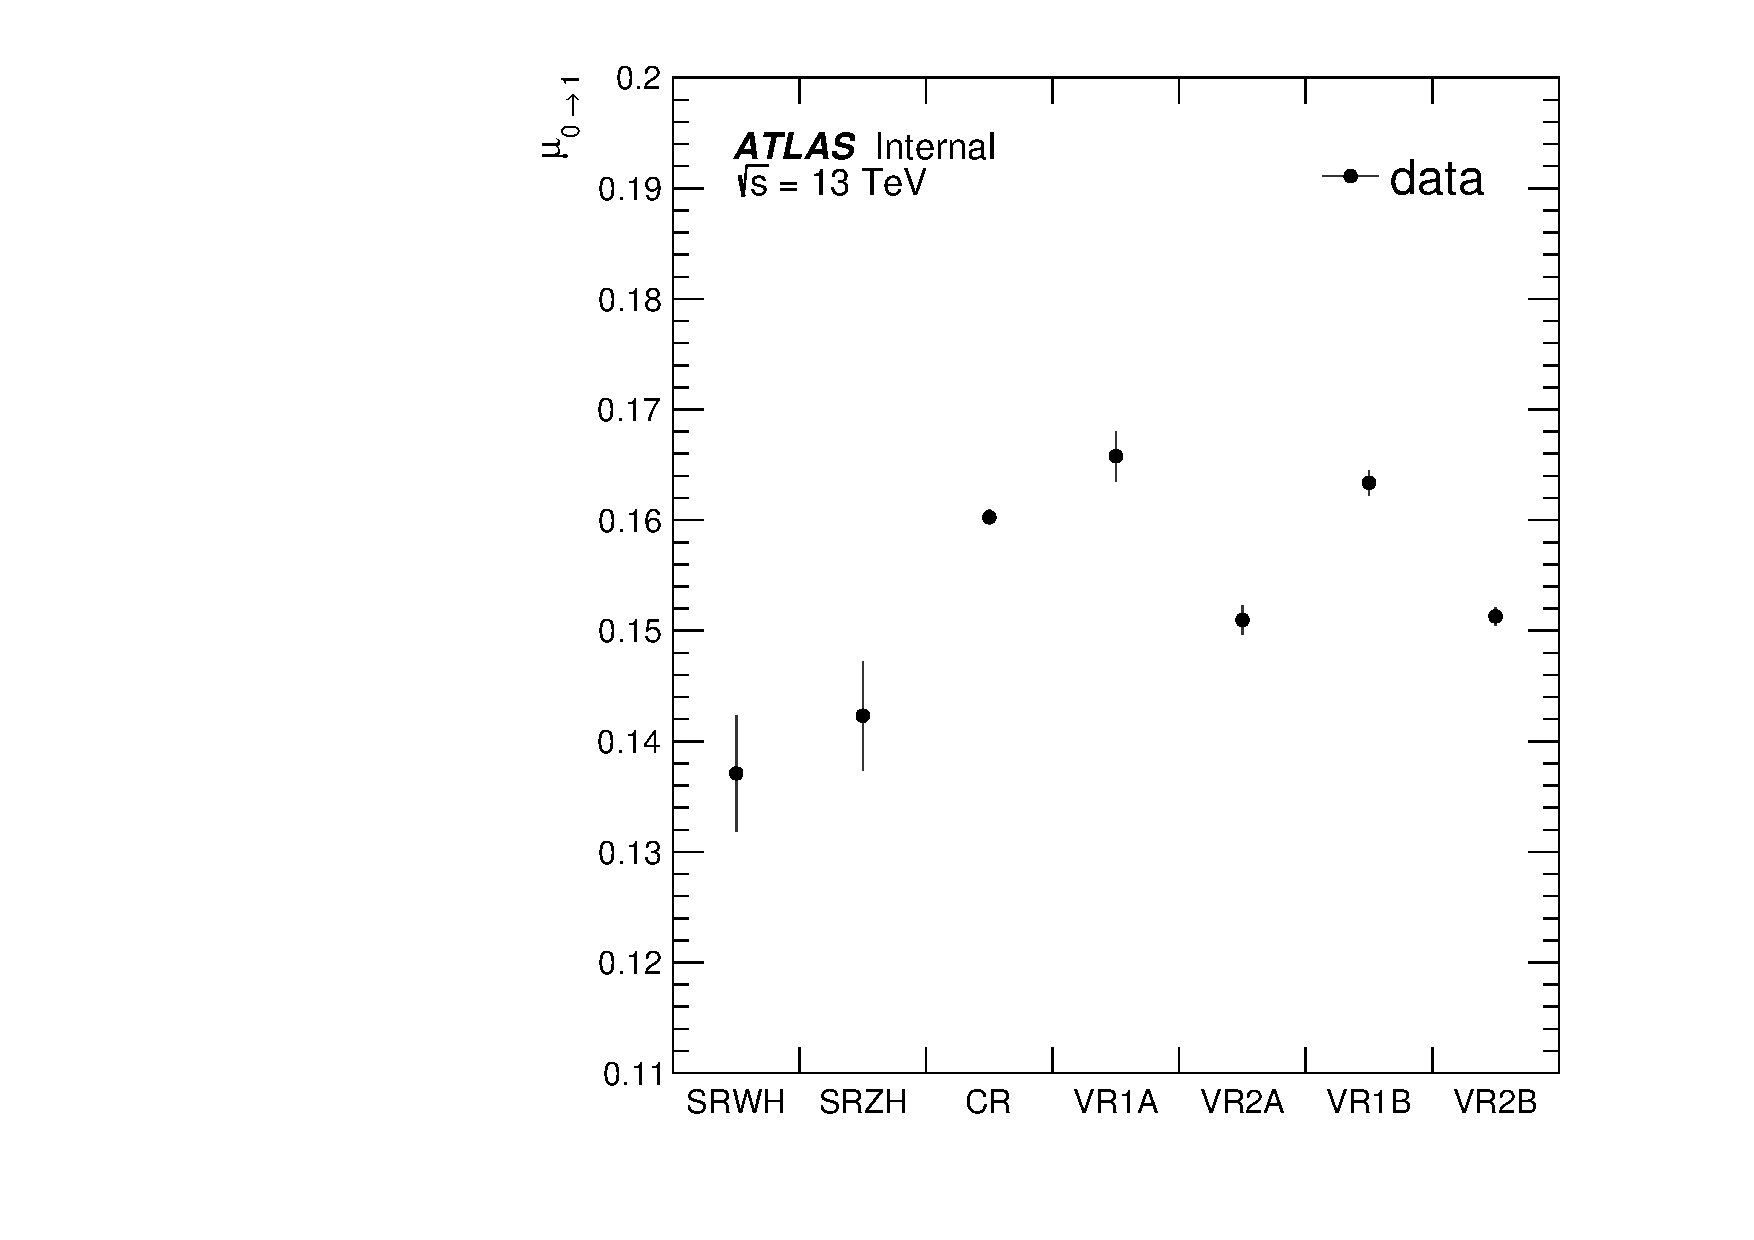
\includegraphics[width=0.49\textwidth]{VHqqbb_PlotRegionMuSF_1tag.pdf}
    \includegraphics[width=0.49\textwidth]{VHqqbb_PlotRegionMuSF_2tag.pdf}
\end{center}
\caption{Observed background normalization scale factor values from data for all regions for 1-tag (left) and 2-tag (right) channels.
    These scale factors ($\mu_{0 \rightarrow N}$) are defined as the ratio of N-tag to 0-tag yield for each particular control/validation/signal region.
}
\label{fig:CompareMu}
\end{figure}

\subsection{Kinematic Re-weighting}
\label{sec:bkg-reweighting}
The 0-tag extrapolation method is based on the assumption that most kinematic variables in the 1-tag or 2-tag channels can be well modeled by the corresponding 0-tag channel.
However, kinematic distributions can be biased when transferring from 0-tag sample to 1/2-tag sample for two main reasons:

\begin{itemize}
    \item \textbf{Non-trivial kinematic dependency of track jets b-tagging efficiency}. Since the track jet b-tagging efficiency strongly depends on the track jet $p_{T}$ (and also some dependency on $\eta$), the kinematic distributions can be sculpted after applying b-tagging requirements.
    \item \textbf{Change of heavy flavor composition}. For example, when moving from 0-tag to 2-tag samples, the fraction of $g\rightarrow bb$ in QCD will increase significantly, which has a different kinematics than the light-quark-dominant 0-tag sample. Similarly, $g \rightarrow c\bar{c}$ fractions are like to differ between 0-tag and 1-tag.
\end{itemize}

A BDT-based approach \cite{BDTrw} has therefore been explored which ensures that the most relevant variables are being used for the reweighting.
In this method a boosted decision tree is used to predict the weights needed to bring the 0-tag and 1/2-tag regions into agreement.
Trees are trained to define single cuts on input variables that maximize the $\chi^{2}$ value between 0-tag and 1/2-tag samples: this will result in a series of regions that are maximally discrepant between the original and the target samples, in other words, regions of phase-space that most need correction in the original sample.

Each leaf in a tree will have an associated weight which depends on the total number of original and target events that it contains, defined during training.
Gradient boosting is performed with a dedicated loss function that gives preference to trees that find such large imbalances between 0-tag and 1/2-tag regions.
The final weight for an event will therefore be a product of weights from each tree, including the chosen learning rate ($\lambda$) as a multiplicative factor.
The hyperparameter values used for this method are described in Table~\ref{tab:bdt_params}.
Open source software based upon scikit-learn~\cite{scikitlearn} was used to perform the re-weighting~\cite{hep_ml:2020arg}.

The following variables are used as inputs to the re-weighting:
\begin{itemize}
    \itemsep -0.5em 
    \item leading track jet $\pt, \eta, \phi, m$ and VR radius
    \item subleading track jet $\pt, \eta, \phi, m$ and VR radius
    \item H/V Candidate Large-R Jet \pt
    \item H Candidate \ntrk
    \item $\left|\Delta R \right|$ between leading/subleading track jet
    \item $\left|\Delta \eta \right|$ between leading/subleading track jet
    \item $\frac{p_T^1}{p_T^1 + p_T^2}$, where $p_T^1$ and $p_T^2$ are the leading/subleading track jet \pt.
    \item Number of track jets ghost-associated to the Higgs candidate
\end{itemize}

\begin{table}[htbp!]
\centering
\begin{scriptsize}
\begin{tabular}{c|c|c}
\hline
BDT Hyperparameter & Value & Description \\
\hhline{|=|=|=|}
Number of Estimators & 100 & Number of base trees in the ensemble used for boosting. \\
\hline
Learning Rate & 0.1 & \makecell{Regularization parameter for the update step of in gradient boosting. \\ Smaller learning rates tend to yield better generalization ability.} \\
\hline
Max Depth & 3 & Maximum depth of the of the base trees. \\
\hline
Min. Samples per Leaf & 500 & \makecell{Minimum number of events allowed in each leaf when \\ determining the cuts that separate leaves in the base trees.} \\
\hline
Subsample & 0.8 & \makecell{Proportion of the training set used for each \\ base tree for 'stochastic' gradient boosting.} \\
\hline
\end{tabular}
\end{scriptsize}
\caption{Summary of BDT hyperparameters used in the re-weighting process.}
\label{tab:bdt_params}
\end{table}

\subsection{Validation}
\label{sec:bkg-validation}

In order to validate the performance of the BDT re-weighting procedure, comparisons to data are studied in the four validation regions: VR1A, VR1B, VR2A, and VR2B.
Figures~\ref{fig:bdt_shape_mVH_1tag} and~\ref{fig:bdt_shape_mVH_2tag} show the \mvh\ distribution in each of these validations for the 1-tag and 2-tag channels, respectively.

One further way of validating the usefulness of the BDT re-weighting is to train binary classifiers using the re-weighting training variables to differentiate between pre and post reweighted data.
Before re-weighting is applied, a properly trained binary classifier should have a (mildly) successful ability to differentiate between, for example, 0-tag and 1-tag.
After re-weighting is applied, a properly trained binary classifier should have little success in distinguishing the re-weighted prediction and the actual 1-tag data, and its application should approach the same result as a random coin flip.
The relative ability of these two classifiers can be quantified by producing Receiver Operating Characteristic (ROC) curves, and these are shown in Figures~\ref{fig:bdt_roc_curves_1tag} and~\ref{fig:bdt_roc_curves_2tag} for 1-tag and 2-tag channels, respectively.
The ability of the two classifiers can be distinguished by computing the area under the ROC curve (AUC), where a random chance classifier would have value of AUC = 0.5.

\begin{figure}[htbp!]
\begin{center}
\includegraphics[width=0.40\textwidth]{BDT/VHqqbbBDTReweightShape_mVH_CR_0tag_to_1tag.pdf} \\
\includegraphics[width=0.40\textwidth]{BDT/VHqqbbBDTReweightShape_mVH_VR1B_0tag_to_1tag.pdf}
\includegraphics[width=0.40\textwidth]{BDT/VHqqbbBDTReweightShape_mVH_VR1A_0tag_to_1tag.pdf} \\
\includegraphics[width=0.40\textwidth]{BDT/VHqqbbBDTReweightShape_mVH_VR2B_0tag_to_1tag.pdf}
\includegraphics[width=0.40\textwidth]{BDT/VHqqbbBDTReweightShape_mVH_VR2A_0tag_to_1tag.pdf}
\end{center}
\caption{\mvh\ predictions for the 1-tag region in all control and validation regions. The predictions shown are constructed by scaling 0-tag data, both before (red) and after (blue) kinematic re-weighting is applied.}
\label{fig:bdt_shape_mVH_1tag}
\end{figure}

\begin{figure}[htbp!]
\begin{center}
\includegraphics[width=0.40\textwidth]{BDT/VHqqbbBDTReweightShape_mVH_CR_0tag_to_2tag.pdf} \\
\includegraphics[width=0.40\textwidth]{BDT/VHqqbbBDTReweightShape_mVH_VR1B_0tag_to_2tag.pdf}
\includegraphics[width=0.40\textwidth]{BDT/VHqqbbBDTReweightShape_mVH_VR1A_0tag_to_2tag.pdf} \\
\includegraphics[width=0.40\textwidth]{BDT/VHqqbbBDTReweightShape_mVH_VR2B_0tag_to_2tag.pdf}
\includegraphics[width=0.40\textwidth]{BDT/VHqqbbBDTReweightShape_mVH_VR2A_0tag_to_2tag.pdf}
\end{center}
\caption{\mvh\ predictions for the 2-tag region in all control and validation regions. The predictions shown are constructed by scaling 0-tag data, both before (red) and after (blue) kinematic re-weighting is applied.}
\label{fig:bdt_shape_mVH_2tag}
\end{figure}

\begin{figure}[htbp!]
\begin{center}
\includegraphics[width=0.49\textwidth]{BDT/VHqqbbBDTRocCurve_VR1A_1tag.pdf}
\includegraphics[width=0.49\textwidth]{BDT/VHqqbbBDTRocCurve_VR1B_1tag.pdf} \\
\includegraphics[width=0.49\textwidth]{BDT/VHqqbbBDTRocCurve_VR2A_1tag.pdf}
\includegraphics[width=0.49\textwidth]{BDT/VHqqbbBDTRocCurve_VR2B_1tag.pdf}
\end{center}
\caption{ Receiver Operating Characteristic (ROC) curves for each validation region in the 1-tag channel. Two separate binary classifiers are trained using a gradient boosted decision tree.
    The red (PRE) line corresponds to the case where no re-weighting has been applied and the classifier is trained to discriminate 0-tag from 1-tag events in each region.
    The blue (POST) line corresponds to the case where re-weighting has been applied and the classifier is trained to discriminate re-weighted 0-tag events from unmodified 1-tag events in each region.
    Each classifier is trained only the set of variables use in the re-weighting.
    In the ideal scenario of perfect re-weighting, the blue line would match very closely to the black line which represents a naive 50/50 random chance classifier.
    The area under the curve (AUC) is shown for each classifier, where a value of 0.5 would correspond to ideal re-weighting.}
\label{fig:bdt_roc_curves_1tag}
\end{figure}

\begin{figure}[htbp!]
\begin{center}
\includegraphics[width=0.49\textwidth]{BDT/VHqqbbBDTRocCurve_VR1A_2tag.pdf}
\includegraphics[width=0.49\textwidth]{BDT/VHqqbbBDTRocCurve_VR1B_2tag.pdf} \\
\includegraphics[width=0.49\textwidth]{BDT/VHqqbbBDTRocCurve_VR2A_2tag.pdf}
\includegraphics[width=0.49\textwidth]{BDT/VHqqbbBDTRocCurve_VR2B_2tag.pdf}
\end{center}
\caption{ Receiver Operating Characteristic (ROC) curves for each validation region in the 2-tag channel. Two separate binary classifiers are trained using a gradient boosted decision tree.
    The red (PRE) line corresponds to the case where no re-weighting has been applied and the classifier is trained to discriminate 0-tag from 2-tag events in each region.
    The blue (POST) line corresponds to the case where re-weighting has been applied and the classifier is trained to discriminate re-weighted 0-tag events from unmodified 2-tag events in each region.
    Each classifier is trained only the set of variables use in the re-weighting.
    In the ideal scenario of perfect re-weighting, the blue line would match very closely to the black line which represents a naieve 50/50 random chance classifier.
    The area under the curve (AUC) is shown for each classifier, where a value of 0.5 would correspond to ideal re-weighting.}
\label{fig:bdt_roc_curves_2tag}
\end{figure}

\subsection{Smoothing}
\label{sec:bkg_fitting}
Due to the small number of events in the tail of the re-weighted background templates, smoothing via fitting with a functional form must be applied to produce a well-behaved background description at high \mvh.
The first step in this process is to derive a well-motivated binning for the \mvh\ histograms based upon the experimental \mvh\ resolution.

First the truth dijet mass ($m_{VH}^{\mathrm{truth}}$) is determined by $\Delta R$-matching both the $H$ and $V$ candidate fat jets to the corresponding \path{AntiKt10TruthTrimmedPtFrac5SmallR20Jets} large radius truth jet collection.
For each WH signal mass value\footnote{No significant different in experimental resolution is observed between simulated WH and ZH signal samples} the residuals ($m_{VH} - m_{VH}^{\mathrm{truth}}$) are fitted with a Crystal Ball function, given by 

\begin{equation}
f(x;\alpha,n,\bar x,\sigma) = N \cdot
    \begin{cases}
        \exp(- \frac{(x - \bar x)^2}{2 \sigma^2}), & \mbox{for }\frac{x - \bar x}{\sigma} > -\alpha \\
        A \cdot (B - \frac{x - \bar x}{\sigma})^{-n}, & \mbox{for }\frac{x - \bar x}{\sigma} \leqslant -\alpha
    \end{cases},
\end{equation}

\begin{align*}
A &= \left(\frac{n}{\left| \alpha \right|}\right)^n \cdot \exp\left(- \frac {\left| \alpha \right|^2}{2}\right),\\
B &= \frac{n}{\left| \alpha \right|}  - \left| \alpha \right|,\\
N &= \frac{1}{\sigma (C + D)},\\
C &= \frac{n}{\left| \alpha \right|} \cdot \frac{1}{n-1} \cdot \exp\left(- \frac {\left| \alpha \right|^2}{2}\right),\\
D &= \sqrt{\frac{\pi}{2}} \left(1 + \operatorname{erf}\left(\frac{\left| \alpha \right|}{\sqrt 2}\right)\right),
\end{align*}
 where $N$ is a normalization factor and $\alpha$, $n$, $\bar x$ and $\sigma$ are parameters which are fitted with the data.

The resulting fitted $\sigma$ parameter from the Crystal Ball function is used a measure of the experimental resolution.
Only events with correct truth-level H/V candidate assignment are considered.
Figure~\ref{fig:mvh_reso_fits} shows the result of this fit for four representative mass points.
The resulting $\sigma$ values are then fit as a linear function of resonance mass, as shown in Figure~\ref{fig:mvh_reso_trend}, and the result is used to derive a set of variable-width bins corresponding to the experimental \mvh\ resolution for the range of 1.3 to 7 TeV.

\begin{figure}[htbp!]
\begin{center}
    \includegraphics[width=0.49\textwidth]{VHqqbb_WH_1400_ResoCrystalBall.pdf}
    \includegraphics[width=0.49\textwidth]{VHqqbb_WH_2500_ResoCrystalBall.pdf} \\
    \includegraphics[width=0.49\textwidth]{VHqqbb_WH_3500_ResoCrystalBall.pdf}
    \includegraphics[width=0.49\textwidth]{VHqqbb_WH_5000_ResoCrystalBall.pdf} \\
\end{center}
\caption{Results for Crystal Ball fits to the HVT WH dijet mass residuals ($m_{VH} - m_{VH}^{\mathrm{truth}}$) for 1.4, 2.5, 3.5 and 5.0 TeV mass values.}
\label{fig:mvh_reso_fits}
\end{figure}

\begin{figure}[htbp!]
\begin{center}
    \includegraphics[width=0.8\textwidth]{VHqqbb_WH_ResoTrendCrystalBall.pdf}
\end{center}
\caption{A linear fit to the \mvh resolution trend as a function of signal resonance mass.
The result of this fit is used to derive a set of variable width bins to utilize for the final input histograms to the statistical framework.}
\label{fig:mvh_reso_trend}
\end{figure}

After the \mvh\ histograms are produced with the variable-binning described above, Eq. \ref{eq:dijet_smooth} is fitted to the prediction for each channel with a three parameter function,
\begin{align}
    \frac{dn}{dx} &= e^{-p_0} \left(1 - x\right)^{-p_1} x^{-p_2},
    \label{eq:dijet_smooth}
\end{align}
where $x = \frac{\mvh}{\sqrt{s}}$ and $p_0$ through $p_2$ are parameters determined by the fit.
The normalization parameter is exponentiated as $e^{-p_0}$ to aid in numerical stability by avoiding very small values for $p_0$.
This functional form models changes in the smoothly falling power-law behavior of the background.
Fits are performed separately for 1-tag and 2-tag channel background estimates for each signal region.

To achieve further numerical stability of the minimization algorithm used by the fit, the histograms are first normalized before fitting.
After fitting, the histograms are re-scaled with the correct propagation of errors applied to both the statistical error of the fit as well as the normalization fit parameter $p_0$.
The fitting method used is a weighted maximum likelihood \footnote{This is achieved by supplying the "WL" option to \path{TH1::Fit}}, due to the fact that the bin contents come from the BDT-reweighted prediction with non-unity event weights.
This replaces the familiar Poisson likelihood with a modified approximate Poisson likelihood based on the number of \textit{effective entries} in each bin, defined as $\left(\sum w_i \right)^2 / \sum w_i^2$, where $w_i$ is the weight of the $i$-th event in the bin.

The error on the fit is computed by taking the eigenvectors of the covariance matrix which describes the errors on the fit parameters.
Each eigenvector is used to produce a new variation of the fit, and the differences between these variations and the nominal are summed in quadrature on a bin-by-bin level to produce the statistical errors associated with the fit as shown by the grey band in Figure~\ref{fig:sr_smoothed}.

The $\frac{\chi^2}{n.d.f.}$ is computed by first rebinning the resulting pre/post-fitted histograms to achieve approximately gaussian statistics in each bin.
This is done by searching the bins upwards, starting from 1.3 TeV, and finding the first bin with a number of effective entries (defined above) below five.
This bin is then merged with all bins above, up to 7 TeV.
The $\frac{\chi^2}{n.d.f.}$ is then computed bin-by-bin with the standard formula.

\begin{table}[!htb]
%\begin{scriptsize}
\begin{center}
\begin{tabular}{|c|c|c|c|c|}
\hline
 & SRWH (1-tag) & SRWH (2-tag) & SRZH (1-tag) & SRZH (2-tag) \\ \hline
    $p_0$ & 14.81 $\pm$ 0.47 & 16.41 $\pm$ 0.34 & 16.21 $\pm$ 0.46 & 17.92 $\pm$ 0.32 \\
\hline
    $p_1$ & 7.59 $\pm$ 0.56 & 4.74 $\pm$ 0.67 & 9.28 $\pm$ 0.53 & 6.74 $\pm$ 0.65 \\
\hline
    $p_2$ & 8.38 $\pm$ 0.11 & 8.28 $\pm$ 0.12 & 9.0 $\pm$ 0.1 & 8.94 $\pm$ 0.12 \\
\hline
    $\chi_{\nu}^2$ & 1.08 & 0.94 & 1.58 & 2.27 \\
\hline
\end{tabular}
\caption{Fitted parameters, parameter errors ($\pm 1 \sigma$), and reduced $\chi^2$ for each signal channel.}
\label{tab:fit_params}
\end{center}
%\end{scriptsize}
\end{table}

\begin{figure}[htbp!]
\begin{center}
\includegraphics[width=0.49\textwidth]{VHqqbb_SmoothedBDT_SRWH_1tag.pdf}
\includegraphics[width=0.49\textwidth]{VHqqbb_SmoothedBDT_SRZH_1tag.pdf} \\
\includegraphics[width=0.49\textwidth]{VHqqbb_SmoothedBDT_SRWH_2tag.pdf}
\includegraphics[width=0.49\textwidth]{VHqqbb_SmoothedBDT_SRZH_2tag.pdf}
\end{center}
\caption{
    The background predictions for \mvh\ after kinematic reweighting and fitting for 1-tag (top row) and 2-tag (bottom row) signal regions.
    The red line shows the final smoothed prediction and the grey band shows the associated statistical error.
    The black points show the pre-smoothed background prediction after kinematic re-weighting, not the actual signal region events.
}
\label{fig:sr_smoothed}
\end{figure}


\section{Statistical Method}
\label{sec:statistics}

A frequentist interpretation of the data is applied via a binned maximum-likelihood (ML) fit performed on the $m_{VH}$ distribution, using the standard package RooStats \cite{Roostats}.
The parameter of interest is the signal strength $\mu$, defined as the scale factor on the total number of signal events predicted by each of the models.
The background only hypothesis corresponds to $\mu = 0$ and the nominal signal plus background hypothesis corresonds to $\mu = 1$.
Histogram templates derived from MC simulation are used for the HVT W' and Z' processes, while the data-driven estimates are used for the combined $t\bar{t}$, $V$+jets, and QCD multijet background.
The input histogram bounds are $[1.3, 6.0]$ TeV, and signal mass points up to 5 TeV are tested.

\subsection{Combined Fit}
\label{sec:combined_fit}
A simultaneous fit is performed to both 1-tag and 2-tag channels, as defined in~\ref{sec:SR}.
This is done separately for each signal region and mass point with the following likelihood formula:

\begin{equation}
L(\mu, \vec{\theta}, \vec{\eta}, \vec{\gamma}) =
\prod_{c=1}^{\mathrm{channels}}\; \prod_{\nu=1}^{\mathrm{bins}}
P_{\mathrm{pois}}\left(N_{c\nu} | \mu s_{c\nu} + b_{c\nu}\right)
\times
\prod_{j \in\,\vec{\theta}} \mathcal{N}(\tilde{\alpha}_{j} | \alpha_{j})
\times
\prod_{k \in\,\vec{\eta}, \vec{\gamma}} \mathnormal{G}(\tilde{\beta}_{k} | \beta_{k})
\end{equation}

where
\begin{itemize}
\itemsep -0.5em
    \item $P_{\mathrm{pois}}$ is the Poisson probability distribution function (PDF).
    \item $N_{c\nu}$ is the observed number of events in the signal region data for the bin $\nu$ in the histogram for channel $c \in$~\{1-tag, 2-tag\}.
    \item $\mu$ is the \textit{signal strength}, a continuous variable that parameterizes a multiplicative factor on the hypothetical signal cross section.
    \item $s_{c\nu}$ is the number of signal events for bin $\nu$ of the histogram for channel $c$.
    \item $b_{c\nu}$ is the expected number of background events for bin $\nu$ of the histogram for channel $c$.
    \item $\vec{\theta}$ is the set of all normalization NPs.
    \item $\vec{\eta}$ is the set of all shape-related NPs.
    \item $\vec{\gamma}$ is the set of NPs denoting the statistical error on the individual bin contents of the signal and background histograms.
    \item $\mathcal{N}(\tilde{\alpha}_{j} | \alpha_{j})$ is the log-normal PDF of the nuisance parameter $\alpha_j$ corresponding to the auxiliary measurement $\tilde{\alpha}_j$.
    \item $\mathnormal{G}(\tilde{\beta}_{k} | \beta_{k})$ is the Gaussian PDF of the nuisance parameter $\beta_k$ corresponding to the auxiliary measurement $\tilde{\beta}_k$.
\end{itemize}

Both $s_{c\nu}$ and $b_{c\nu}$ themselves depend upon a subset of the nuisance parameters $\vec{\theta}$ and $\vec{\eta}$ as described in section~\ref{sec:syst}.
Nuisance parameters which produce bin variations which are smaller than 1\% with respect to the nominal bin contents are pruned away.
For each bin in each histogram, interpolation must be performed between the nominal bin prediction and the variations induced by the nuisance parameters to produce the actual value of $s_{c\nu}$ and $b_{c\nu}$ used to compute the likelihood.
Details on the benefits and drawbacks of various interpolation options, as well as the default options used here, are discussed in~\cite{HistFactory2012}.

\subsection{Upper Limits on Cross Section}
Upper limits on the signal strength $\mu$ are set using a modified frequentist method ($CL_s$)~\cite{Read:451614}.
The values $CL_{s+b}$ and $CL_b$ are computed using an asymptotic method~\cite{asymptotics} and correspond to the p-values for the signal-plus-background and background-only hypothesis, respectively.
Limits at 95\% confidence level on the signal strength can be computed by (1) scanning values of $\mu$ (2) computing $CL_s$ and (3) identifying $\mu_{0.05}$ (the value of $\mu$ at which $CL_s$ = 0.05).

For the calculation of the p-values used in this computation, a test statistic $\lambda(\mu)$ is defined as a profile-likelihood ratio:
\[ \lambda(\mu) = \begin{cases}
    -2 \ln{\frac{L(\mu, \hat{\hat{\Theta}}(\mu)}{L(\hat{\mu}, \hat{\Theta})}}, & 0 \leq \hat{\mu} \leq \mu \\
        0, & \hat{\mu} > \mu \\
    -2 \ln{\frac{L(0, \hat{\hat{\Theta}}(0)}{L(\hat{\mu}, \hat{\Theta})}}, & \hat{\mu} < 0 \\
   \end{cases}
\]
where $L$ is the likelihood and $\Theta \equiv \{\vec{\theta}, \vec{\eta}, \vec{\gamma}\}$ is the full set of all nuisance parameters, all described in~\ref{sec:combined_fit}.
The global best fit values for $\mu$ and $\Theta$ are denoted $\hat{\mu}$ and $\hat{\Theta}$, while the best fit values of $\Theta$ for a particular value of $\mu$ are denoted $\hat{\hat{\Theta}}(\mu)$.
This ratio of likelihoods, for the case of a given $\mu$ hypothesis, quantities the compatibility of the data with such a hypothesis.

\section{Systematic Uncertainties}
\label{sec:syst}

This section describes the sources of systematic uncertainty considered in this analysis, which are divided into two main categories: experimental uncertainties, which impact only the signal distributions because the background is data-driven, and the uncertainties in the modelling of the background estimate. The impact of these uncertainties is estimated on the final discriminant variable ($m_{JJ}$).

\subsection{Experimental Uncertainties}
\label{sec:syst-exp}
%\input{sections/syst-bkg.tex}
\subsubsection{Luminosity Uncertainty}
The uncertainty in the combined 2015--2018 integrated luminosity is 1.7\% \cite{ATLAS-CONF-2019-021}, obtained using the LUCID-2 detector \cite{LUCID2} for the primary luminosity measurements.
This uncertainty is applicable only to the simulated signal samples and has only a small impact on this analysis.

\subsubsection{Large-$R$ Jet $p_T$ scale and resolution}
Uncertainty in the jet \pt\ scale (JpTS) is an important uncertainty to consider in any search for resonant structures with a smoothly falling dijet background.
The effect of this uncertainty manifests as a shift in the peak of the expected signal mass spectrum, which alters the significance of any observed excess.
The uncertainties on the jet \pt\ scale (JpTS) are evaluated by the combined performance groups using track-to-calorimeter double ratios between data and MC.
Discrepancies observed between data and MC are assigned as uncertainties on the \pt\ scale of the jet.

%The details of this procedure are summarized in detail on the JetEtmiss twiki\footnote{\url{https://twiki.cern.ch/twiki/bin/viewauth/AtlasProtected/RTrackUncertaintyGuide}}.
The ratio of the two measures of jet \pt\ (calorimeter-based and track-based) is expected to be the same (though not equal to one) in both data and MC.
Any observed differences are assigned as baseline systematic uncertainties.
Additional uncertainties due to the reconstruction and modelling of tracks are taken into account as well.
These uncertainties are taken from the inner detector group tools and cover track reconstruction efficiency, impact parameter resolution, tracking in dense environments, track fake rate, and sagitta biases.
The size of the total JpTS uncertainty (including baseline ratio, statistical, and tracking uncertainties) varies with jet \pt\ and is around 5\% to 10\% for the full mass range.
The uncertainties are computed in bins of $\frac{m_{jet}}{p_T^{jet}}$ and $\eta$, with one typical example result shown in Figure~\ref{fig:tcc_rtrk}.
%The following jet \pt\ scale variations are used:
%\begin{enumerate}
%    \itemsep -1em 
%    \item \path{FATJET_JET_Rtrk_Baseline_pT}
%    \item \path{FATJET_JET_Rtrk_Closure_pT}
%    \item \path{FATJET_JET_Rtrk_Modelling_pT}
%    \item \path{FATJET_JET_Rtrk_TotalStat_pT}
%    \item \path{FATJET_JET_Rtrk_Tracking_pT}
%\end{enumerate}

Due to the unique track-influenced nature of TCC jets, the impact of possible correlations between track-based \pt\ and calo-based \pt\ were studied by considering a data/MC comparison method between calo-based (LCTopo) jets and TCC jets.
The results are shown in Figure~\ref{fig:tcc_lctopo_calib}, and the observed discrepancy was found to have a maximum value of 2\% and the effect is thus ignored.

Uncertainties due to jet \pt\ measurement resolution (JpTR) would lead to a mis-measurement of the width of any observed signal and impact the signal selection efficiency.
Additional uncertainties due to the jet energy are estimated by applying a Gaussian smearing which degrades the nominal \pt\ resolution of jets by an absolute 2\%. %as recommended by the JetMet working group\footnote{\url{https://twiki.cern.ch/twiki/bin/viewauth/AtlasProtected/JetUncertainties2016Moriond2017\#Resolution_uncertainties}}.
The changes to the overall yield and \mvh\ shape are then assigned as  'up' variations, and the corresponding 'down' variation is taken by mirroring the difference between the nominal and 'up' variations.

\begin{figure}[htbp!]
\begin{center}
\includegraphics[width=0.45\textwidth]{JpTS_TCC_m90.png}
\includegraphics[width=0.45\textwidth]{JMS_TCC_m90.png}
\end{center}
\caption{Fractional jet \pt\ scale (left) and mass scale (right) systematic uncertainty components for anti-$k_t$, $R=1.0$ TCC jets in the $\eta = 0$ and $m = 90$ GeV bin, using the TCC+JES+JMS calibration scheme.
    The total uncertainty (all components summed in quadrature) is shown as a filled blue region topped by a solid black line.
}
\label{fig:tcc_rtrk}
\end{figure}

\begin{figure}[htbp!]
\begin{center}
\includegraphics[width=0.7\textwidth]{tcc_track_calo_correlation.png}
\end{center}
\caption{Average ratio of jet \pt\ for TCC jets to jet \pt\ for LCTopo jets as a function of \pt\ for anti-$k_t$ $R=1.0$ jets with $|\eta| < 2$.
© CERN
}
\label{fig:tcc_lctopo_calib}
\end{figure}

\subsubsection{$b$-tagging Uncertainties}
The uncertainties related to the b-tagging efficiency calibrations as measured in $t\bar{t}$ events for track-jets are considered, using the official ATLAS prescriptions~\cite{Aad:2019aic, Aaboud:2018xwy}.
These uncertainties result from three broad categories: \textit{MC generator modelling uncertainty} which impact the kinematic distributions and jet flavour composition in simulated events, \textit{normalisation uncertainty} which account for uncertainties in the cross-section of simulated samples, and \textit{experimental uncertainties} which cover uncertainties in detector effects and reconstruction of physics objects.

These uncertainties enter the analysis through variations on the b-tagging simulation-to-data scale factors.
The number of systematic variations is ultimately reduced by summing together the covariance matrices (with respect to jet \pt) for each variation and computing the eigenvectors of this total covariance matrix.
%This results in the following 13 variations on the simulation-to-data scale factors:
%\begin{enumerate}
%    \itemsep -1em 
%    \item \path{FT_EFF_Eigen_B_0_AntiKtVR30Rmax4Rmin02TrackJets}
%    \item \path{FT_EFF_Eigen_B_1_AntiKtVR30Rmax4Rmin02TrackJets}
%    \item \path{FT_EFF_Eigen_B_2_AntiKtVR30Rmax4Rmin02TrackJets}
%    \item \path{FT_EFF_Eigen_C_0_AntiKtVR30Rmax4Rmin02TrackJets}
%    \item \path{FT_EFF_Eigen_C_1_AntiKtVR30Rmax4Rmin02TrackJets}
%    \item \path{FT_EFF_Eigen_C_2_AntiKtVR30Rmax4Rmin02TrackJets}
%    \item \path{FT_EFF_Eigen_C_3_AntiKtVR30Rmax4Rmin02TrackJets}
%    \item \path{FT_EFF_Eigen_Light_0_AntiKtVR30Rmax4Rmin02TrackJets}
%    \item \path{FT_EFF_Eigen_Light_1_AntiKtVR30Rmax4Rmin02TrackJets}
%    \item \path{FT_EFF_Eigen_Light_2_AntiKtVR30Rmax4Rmin02TrackJets}
%    \item \path{FT_EFF_Eigen_Light_3_AntiKtVR30Rmax4Rmin02TrackJets}
%    \item \path{FT_EFF_extrapolation_AntiKtVR30Rmax4Rmin02TrackJets}
%    \item \path{FT_EFF_extrapolation_from_charm_AntiKtVR30Rmax4Rmin02TrackJets}
%\end{enumerate}

\subsubsection{Boson Tagging Uncertainties}
\label{sec:syst-boson}
%TODO: describe VVJJ method
Additional uncertainties related to boson tagging can impact both the V/H tagging efficiency as well as the resulting dijet mass shape.
These uncertainties include jet mass scale (JMS), jet mass resolution (JMR), jet \d2 resolution (D2R) and uncertainties due to the \ntrk variable.
The JMR and JMS systematic uncertainties for TCC jets are officially provided by ATLAS Jet working group and included in the analysis.
Since vector boson tagging and Higgs boson tagging implement different selections using different observables, a separate description of the signal systematic uncertainties related to the two taggers is provided in the following paragraphs.
In the end the V boson and H boson systematics are treated as uncorrelated.

\subsubsection{Vector boson tagging scale factor and uncertainties}
\label{sec:syst-vec-boson}
As already described in Section~\ref{subsec:tagger_opt}, this analysis uses a modified version of the 3 variables (jet mass, \d2, and \ntrk) vector-boson tagger optimised by the fully-hadronic diboson resonance search team for the full Run-2 paper~\cite{VVJJPaper2019}. Jet invariant mass and \d2 selections follow exactly the same definitions as the ones used in the fully hadronic diboson resonance search, while the \ntrk selection has been loosened by the maximum sensitivity optimisation performed for the event selection of this analysis.
Given the shape of the \ntrk distribution for vector bosons, a small change in the \ntrk selection (VH allows on average 3 more tracks than VVJJ for both W-boson and Z-boson selection) produces a small and almost linear change in signal efficiency.
For this reason, the same boson tagging scale factor and relative systematic uncertainty derived in the VVJJ analysis is applied in this analysis.
In particular, a data-to-MC SF of $0.92\pm0.13$ is applied to our MC signals, which was derived via studies of W/Z tagging in real $V$+jets events in data/MC. The 0.13 is considered as signal normalisation scale factor uncertainty. It includes high \pt\ extrapolation, modelling uncertainties, impact of jet mass scale and resolution, and fitting uncertainties.

\subsubsection{Systematic uncertainties for Higgs tagging}
\label{sec:syst-h-boson}
Given the very small cross section of the Higgs boson, it is not possible to define a H+jets control region where a data-to-MC H-tagging scale factor for \ntrk selection can be evaluated.
In the 2017 fully hadronic diboson resonance search ~\cite{VVJJPaper2017}, a $1.03\pm0.05$ data-to-MC scale factor for \ntrk in vector bosons has been measured in a V+jets control region.

Summing in quadrature the $3\%$ scale factor with the $5\%$ systematic uncertainty, the fully hadronic diboson resonance search considered a conservative 6\% data-to-MC scale factor for the \ntrk variable.
The impact of this scale factor on the signal normalisation was observed to be approximately 13\%.
In the case of applying this result to the \ntrk selection for H-tagging in this analysis, the 13\% result obtained for V-tagging is not directly applicable: phase-space and topology differences need to be taken into account.
In order to quantify these differences and assess additional uncertainties for this particular selection, an \ntrk double ratio has been defined as a function of the jet mass.
Eq.~\ref{eq:doubleratio} shows the definition of this quantity:

\begin{align}
    R_{\mathrm{ntrk}} &=
    \frac{
        \frac{ \mathrm{jet}_m^{\mathrm{data}} | \mathrm{w/o}~\ntrk }
        { \mathrm{jet}_m^{\mathrm{MC}}| \mathrm{w/o}~\ntrk}
        }
        { \frac{\mathrm{jet}_m^{\mathrm{data}}| \mathrm{w/}~\ntrk}{\mathrm{jet}_m^{\mathrm{MC}}| \mathrm{w/} ~\ntrk} }
    \label{eq:doubleratio}
\end{align}

The purpose of the $R_{\mathrm{ntrk}}$ quantity is to compare the jet mass distributions for the mass range [60,150] GeV\ in both data and multijet MC samples, with and without applying the \ntrk selection.
This comparison has been repeated for different b-tagging conditions in order to check the impact on $R_{\mathrm{ntrk}}$ produced by the correlation between \ntrk and b-tagging.
Figure~\ref{fig:double_ratio} shows $R_{\mathrm{ntrk}}$ for different b-tagging selections.
A 2\% difference between the ratio in the Vector boson (red line) and Higgs boson (yellow line) jet mass regions is visible in the top-left plot.
This difference can be partially explained by the presence of real W/Z bosons in data that are not included in QCD MC.
Both 1-tag (top-right) and 2-tag (bottom plot) channels do not show differences larger that 1\%.
In order to be conservative while evaluating this difference only on background dominated samples, the 2\% observed difference in $R_{\mathrm{ntrk}}$ is inflated up to 5\% and then added in quadrature to the original 6 $\%$ data-to-MC \ntrk scale factor obtained on 2015-2016 data in V+jets control region.
This resulting \ntrk\ uncertainty from Higgs tagging resolves to a 10\% signal normalisation uncertainty.
Any shape effects on the signal peak due to the \ntrk scale factor are considered as negligible.


\begin{figure}[htbp!]
\begin{center}
    \includegraphics[width=0.49\textwidth]{anybtag.pdf}
    \includegraphics[width=0.49\textwidth]{1btag.pdf} \\
    \includegraphics[width=0.49\textwidth]{2btag.pdf}
%    \includegraphics[width=0.49\textwidth]{./figures/Tagging/VHqqbbOptimizedBosonTagger_H_ntrk_2tag.pdf}
\end{center}
\caption{$R_{\mathrm{ntrk}}$ for different inclusive b-tagging (top-left), 1 b-tagging (top-right), and 2 b-tagging (bottom) selections. The red and yellow lines in the ratio panels show the average $R_{\mathrm{ntrk}}$ values for the vector- and Higgs- boson mass windows, respectively.}
\label{fig:double_ratio}
\end{figure}

\subsubsection{Large-R Jet Mass Resolution}
%The official JetEtMiss tool is used to produce TCC jet mass resolution variations.
Jet mass resolution variations are produced by randomly smearing the jet mass by 20\% relative to the nominal resolution, using resolution maps provided by the ATLAS jet working group under the assumption of different jet truth origin.
For this analysis, the maps for $H \rightarrow b\bar{b}$ large-$R$ jets are used.
A comparison of TCC vs. LCTopo large-R Higgs jet mass resolution is shown in Figure~\ref{fig:jmr_higgs}, produced with the signal samples from this analysis.

\begin{figure}[htbp!]
\begin{center}
\includegraphics[width=0.7\textwidth]{JMR_Higgs_TCC.pdf}
\end{center}
\caption{
    Fractional Jet Mass Resolution (JMR) for truth Higgs jets with pre-selection applied.
    The JMR is computed here from a Gaussian fit, as opposed to the method from JetEtMiss utilizing the interquartile range (IQR).
    This yields a larger, more conservative value for the JMR.
    © CERN
}
\label{fig:jmr_higgs}
\end{figure}

\subsubsection{$\mu$ Uncertainty}
The uncertainty on the background normalization estimate from statistical as well as non-closure related uncertainty is described in Section \ref{sec:bkg-normalization}.

\subsubsection{BDT Re-Weighting Uncertainty}
The BDT re-weighting algorithm is trained in the control region (CR) and applied to the validation and signal regions.
To account for the uncertainty in this extrapolation, a shape systematic uncertainty is derived by applying the background fitting method outlined in Section~\ref{sec:bkg_fitting} to both the BDT re-weighted prediction as well as the actual data in a particular validation region (VR2B) chosen due to the high event yield.
The ratio of the smoothed fits of the BDT prediction and data, shown in Figure~\ref{fig:bdt_shape_syst}, is used to produce \mvh-dependent weights.
These weights are then used to produce up/down shape variations for each signal region and channel.
The predominant effect of this uncertainty manifests in the high \mvh\ tail.
To allow more flexibility in the likelihood fit, this systematic is split into two separate low/high mass regions below/above 2.5 TeV.

%TODO: replace separate bkg. shape uncertainty plots with updated combined plots from paper aux. material
\begin{figure}[htbp!]
\begin{center}
\includegraphics[width=0.49\textwidth]{VHqqbb_BDTShapeSystematic_VR2B_1tag.pdf}
\includegraphics[width=0.49\textwidth]{VHqqbb_BDTShapeSystematic_VR2B_2tag.pdf}
\end{center}
\caption{Separate smoothing results for the BDT re-weighted prediction (red) as well as data (blue) for the 1-tag (left) and 2-tag (right) channels in the VR2B validation region.
    The ratio panel shows the ratio of these two predictions, which is used to derive \mvh\ dependent weights which are subsequently used to produce up/down variations for each signal region/channel to account for uncertainty in the shape effects resulting from the BDT re-weighting procedure.
}
\label{fig:bdt_shape_syst}
\end{figure}

\subsubsection{Background Smoothing Function Choice Uncertainty}
Systematic uncertainty due to the choice of fit function is considered by applying the same method described in Section~\ref{sec:bkg_fitting}, but with a different smoothing function: $e^{-p_0} \left(1 - x\right)^{-p_1} \left(1+x\right)^{-p_2 \log{x}}$.
Results are shown in Figure~\ref{fig:sr_smoothed_variation}.
To allow more flexibility in the likelihood fit, this systematic uncertainty is split into two separate low/high mass regions below/above 2.5~TeV.

\begin{figure}[htbp!]
\begin{center}
\includegraphics[width=0.49\textwidth]{VHqqbb_AltSmoothedBDT_SRWH_1tag.pdf}
\includegraphics[width=0.49\textwidth]{VHqqbb_AltSmoothedBDT_SRZH_1tag.pdf} \\
\includegraphics[width=0.49\textwidth]{VHqqbb_AltSmoothedBDT_SRWH_2tag.pdf}
\includegraphics[width=0.49\textwidth]{VHqqbb_AltSmoothedBDT_SRZH_2tag.pdf}
\end{center}
\caption{Smoothing fit function variations produced with the alternative fit function: $e^{-p_0} \left(1 - x\right)^{-p_1} \left(1+x\right)^{-p_2 \log{x}}$.}
\label{fig:sr_smoothed_variation}
\end{figure}

\subsection{Theory Uncertainties}

\subsubsection{Parton Distribution Function Uncertainties}
\label{sec:pdf_unc}
Uncertainties in the behavior of the parton distribution functions at the high $Q^2$ values explored in this analysis can potentially have a large effect on the production rate of any signal.
This systematic uncertainty is derived by applying the methodology outlined by the PDF4LHC group using event-level re-weighting\footnote{https://lhapdf.hepforge.org} to four additional PDF sets\footnote{CT14, MMHT2014, NNPDF3.0, and ATLAS-epWZ12}.

Any systematic error introduced due to PDF variations must be reported as an uncertainty on the signal acceptance rather than the signal cross section. The acceptance is defined as
$\frac{\sum_{\mathrm{weights}} (\mathrm{signal\ selection})}{\sum_{\mathrm{weights}} (\mathrm{no\ selection})}$.
The uncertainty on signal acceptance is estimated by computing variations in the acceptance ratio, defined as the ratio between the acceptance for a particular PDF variation and the nominal acceptance.
The PDF \textit{variations} here can be either a comparison to different PDF sets, as well as comparisons to variations in the error sets of the nominal PDF.
For all signal regions and mass points the impact was shown to be less than 1\%, so no uncertainties due to PDF variations are included in the results.

\subsubsection{ISR/FSR Uncertainties}

Any choice of MC tune merits the use of additional systematic uncertainties to cover variations in Initial State Radiation (ISR), Final State Radiation (FSR), and Multi-Parton Interactions (MPI).
The expected effect on signal efficiency is evaluated at truth level before applying boson tagging cuts, following the same procedure as for the PDF variations described above.

The impact on signal acceptance is demonstrated in Figure~\ref{fig:isr_fsr_impact}.
In the final results a flat systematic uncertainty on the signal normalization of 2\%(3\%) for WH(ZH) is used.

\begin{figure}[htbp!]
\begin{center}
\includegraphics[width=0.49\textwidth]{VHqqbb_ISR_FSR_Eff_Variation_WH.pdf}
\includegraphics[width=0.49\textwidth]{VHqqbb_ISR_FSR_Eff_Variation_ZH.pdf}
\end{center}
\caption{
    Impact on signal acceptance $\times$ efficiency vs. resonance mass for each of the ISR/FSR tune variations under consideration.
}
\label{fig:isr_fsr_impact}
\end{figure}
